\documentclass[11pt]{book}

\usepackage{emptypage}

\usepackage[utf8x]{inputenc}
\usepackage{listings}
\usepackage{hyperref}
\usepackage{exercise}

\usepackage{algorithm}
\usepackage{algorithmicx}
\usepackage[noend]{algpseudocode}

\usepackage[toc,page]{appendix}

\usepackage[secthm,mdthm]{evan}

\usepackage{answers}

\lhead{Samuel Hsiang, Alexander Wei}

\usepackage{graphicx}

\usepackage{color}

\definecolor{myseagreen}{RGB}{88,197,191}
\definecolor{mysalmon}{RGB}{255,160,122}
\definecolor{myred}{RGB}{255,102,102}
\definecolor{mypurple}{RGB}{225,145,255}
\definecolor{myblack}{RGB}{0,0,0}
\definecolor{mywhite}{RGB}{255,255,255}

\usepackage{tikz}

\usetikzlibrary{calc,shapes.multipart,chains,arrows,positioning}

\tikzstyle{vertex}=[draw,fill=myseagreen,circle,minimum size=24pt,inner sep=0pt]

\tikzstyle{splitvertex}=[draw,fill=myseagreen,circle split,minimum size=24pt]

\usetikzlibrary{
  shapes.multipart,
  matrix,
  positioning,
  shapes.callouts,
  shapes.arrows,
  shapes.geometric,
  decorations.shapes,
  shapes,
  fit,
  arrows,
  positioning,
  trees,
  mindmap,
  calc}

\tikzset{
    squarecross/.style={
        draw, rectangle,minimum size=18pt, fill=myseagreen,
        inner sep=0pt, text=black,
        path picture = {
            \draw[black]
            (path picture bounding box.north west) -- 
            (path picture bounding box.south east)
            (path picture bounding box.south west) -- 
            (path picture bounding box.north east);
        }
    }
}

\lstset{language=Java}
 
\definecolor{codegreen}{rgb}{0,0.6,0}
\definecolor{codegray}{rgb}{0.5,0.5,0.5}
\definecolor{codepurple}{rgb}{0.58,0,0.82}
\definecolor{backcolour}{rgb}{0.95,0.95,0.92}

\lstnewenvironment{mylstlisting}[1][]%
  {\noindent\minipage{\linewidth}\medskip 
   \lstset{
    backgroundcolor=\color{backcolour},   
    commentstyle=\color{codegreen},
    keywordstyle=\color{magenta},
    numberstyle=\tiny\color{codegray},
    stringstyle=\color{codepurple},
    basicstyle=\footnotesize,
    breakatwhitespace=false,         
    breaklines=true,                 
    captionpos=t,                    
    keepspaces=true,                 
    numbers=left,                    
    numbersep=5pt,                  
    showspaces=false,                
    showstringspaces=false,
    showtabs=false,                  
    tabsize=4,
   basicstyle=\ttfamily\footnotesize,
   frame=single,#1}}
  {\endminipage}

\raggedbottom

% \includeonly{chapters/fundamentals}

\begin{document}

\frontmatter

\title{Crash Course Coding Companion}
\author{
Samuel Hsiang \\ 
Thomas Jefferson High School for Science and Technology \\ 
\href{mailto:samuel.c.hsiang@gmail.com}{\texttt{\textup{samuel.c.hsiang@gmail.com}}} \\
\vspace{.7em}
Alexander Wei \\
Phillips Exeter Academy
}
\date{\today}

\maketitle

\newpage
~\vfill
\thispagestyle{empty}

% \noindent Copyright \copyright\ 2013 John Smith\\ % Copyright notice

\noindent Copyright, publishing, and licensing information should go here. I don't have anything fancy like that. It is of my (na\"{i}ve, privileged teenager) belief that knowledge should be free and easily accessible to ambitious high schoolers, but it is paramount to respect intellectual property and someone else's work. I ask that you use this material to its fullest potential, however you like, provided it doesn't completely butcher the philosophy with which I embarked on this project.

\begin{flushright}
-- Samuel
\end{flushright}

% \noindent \textsc{Published by Publisher}\\ % Publisher

% \noindent \textsc{book-website.com}\\ % URL

\noindent \url{https://www.dropbox.com/s/z2lur71042pjaet/guide.pdf?dl=0}

\noindent \url{https://github.com/alwayswimmin/cs_guide}

% \noindent Licensed under the Creative Commons Attribution-NonCommercial 3.0 Unported License (the ``License''). You may not use this file except in compliance with the License. You may obtain a copy of the License at \url{http://creativecommons.org/licenses/by-nc/3.0}. Unless required by applicable law or agreed to in writing, software distributed under the License is distributed on an \textsc{``as is'' basis, without warranties or conditions of any kind}, either express or implied. See the License for the specific language governing permissions and limitations under the License.\\ % License information

% \noindent \textit{First printing, March 2013} % Printing/edition date

\newpage
\thispagestyle{empty}
\par\vspace*{.35\textheight}{\centering For Rachel \par}


\chapter{Acknowledgments}

I am truly thankful for all my school teachers and USACO instructors, who gave me the knowledge which I wish to pass on through this text. I am grateful for Shankar and Ross, Evan, and Dr. Osborne, who separately made me believe such a task was possible. I must credit Valerie, for she was the one who drove me to really dive into and come to love computer science. Shwetark were extremely helpful with writing this text, as they provided input and helped me find problems to supplement my work. Lastly, huge shoutouts to Alex, who has been tremendous as a partner in writing this! Finally, I'd like to thank all my friends and avid programmers in the TJ community. This is for all of you, and I hope you find it useful in your studies.

\begin{flushright}
-- Samuel
\end{flushright}

\tableofcontents

\listofalgorithms

\chapter{Preface}

You might have heard of \href{https://www.dropbox.com/s/z8qdndxmrmxqsam/Napkin.pdf?oref=e&n=97419869}{Evan Chen's Napkin}, a resource for olympiad math people that serves as a jumping point into higher mathematics.\footnote{In fact, I'm using Evan's template right now. Thanks Evan!} The Wikipedia articles on higher mathematics are just so dense in vocabulary and deter many smart young students from learning them before they are formally taught in a course in college. Evan's Napkin aims to provide that background necessary to leap right in.

I feel the same way about computer science. For most, the ease of the AP Computer Science test means that the AP coursework is often inadequate in teaching the simplest data structures, algorithms, and big ideas necessary to approach even silver USACO problems. On the other hand, even the best reference books, like Sedgewick, are too dense and unapproachable for someone who just wants to sit down and learn something interesting.\footnote{Sedgewick, notably, is getting better. \href{http://algs4.cs.princeton.edu/home/}{Check out his online companion} to \textit{Algorithms, 4th Edition}.} The road, for many, stalls here until college. Everyone should be able to learn the simplest data structures in Java or C++ standard libraries, and someone with problem-solving experience can easily jump right into understanding algorithms and more advanced data structures.

A few important notes, before we begin.

\begin{itemize}

\item

I'm assuming some fluency in C-style syntax. If this is your first time seeing code, please look somewhere else for now.

\item

It is essential that you understand the motivations and the complexities behind everything we cover. I feel that this is not stressed at all in AP Computer Science and lost under the heavy details of rigorous published works. I'm avoiding what I call the heavy details because they don't focus on the math behind the computer science and lose the bigger picture. My goal is for every mathematician or programmer, after working through this, to be able to code short scripts to solve problems. Once you understand how things work, you can then move on to those details which are necessary for building larger projects. The heavy details become meaningless as languages develop or become phased out. The math and ideas behind the data structures and algorithms will last a lifetime.

\item

It is recommended actually code up each data structure with its most important functions or algorithm as you learn them. I truly believe the only way to build a solid foundation is to code. Do not become reliant on using the standard library (\texttt{java.util}, for instance) without understanding how the tool you are using works.

\end{itemize}


\mainmatter

\chapter{Fundamentals}

\section{Input and Output}

The first part of solving any programming contest problem is reading the input correctly. In this section, we'll briefly go over input and output in Java using \texttt{java.util.Scanner} and \texttt{java.io.PrintWriter}. There are two scenarios that you should be familiar with: \texttt{stdin}/\texttt{stdout} and file I/O. You encounter the former when you enter input and see output for a program run in the commandline. You encounter the latter when you have two files (for example \texttt{input.txt} and \texttt{output.txt}) that you read from and write to.

When using \texttt{stdin}/\texttt{stdout}, we read input from \texttt{System.in} using a Scanner and output our results using \texttt{System.out.println()}. \texttt{Scanner.nextInt()} and \texttt{Scanner.next()} read in integers and strings, respectively. \texttt{System.out.println()} prints its argument and adds a newline at the end. (If we don't want the newline, we can use \texttt{System.out.print()}.) Here's an example of a main method that takes two integers and outputs their sum:

\begin{mylstlisting}
public static void main(String args[]){
  // hint: you should write "import java.util.*;" at the top of your code.
  Scanner sc = new Scanner(System.in);
  int x = sc.nextInt();
  int y = sc.nextInt();
  System.out.println(x + y);
}
\end{mylstlisting}

File I/O is a touch more complicated. For our Scanner, we have to make a new File object and use it in the constructor. We do the same for our PrintWriter. However, PrintWriter also comes with a couple more usage notes. First, we should include \texttt{throws IOException} after our main method, since Java requires that we acknowledge the possibility of an IOException. (We bravely assume that our file open will succeed!) After we finish printing, we must also close the PrintWriter to make sure that everything gets written. Here's a snippet showing how Scanner and PrintWriter work with files: 

\begin{mylstlisting}
public static void main(String args[]) throws IOException {
  // hint: for file I/O, you should also have "import java.io.*;"
  Scanner sc = new Scanner(new File("input.txt"));
  int x = sc.nextInt();
  int y = sc.nextInt();
  PrintWriter pw = new PrintWriter(new File("output.txt"));
  pw.println(x + y);
  pw.close();
}
\end{mylstlisting}

Although more efficient methods of I/O exist, such as BufferedReader and BufferedWriter, what's covered here should be sufficient for now. (It's possible to read in $10^5$ integers with Scanner in a fraction of a second.)

Now that we can read and write, let's move on to one of the most basic subroutines in computer science: sorting. 

\section{Comparable}

We'll start by taking a look at how Java sorts objects. In \texttt{java.util.Arrays}, there is a built-in sort method, \texttt{Arrays.sort()}, which takes an array and sorts it. If we want to sort an array of our own objects, we have to first implement the \texttt{Comparable} interface. This is how Java orders a set of objects. Implementing \texttt{Comparable} requires support of the method \texttt{int compareTo(Object o)}. If \texttt{a.compareTo(b) < 0}, then \texttt{a} comes before \texttt{b}; if \texttt{a.compareTo(b) > 0}, then \texttt{a} comes after \texttt{b}; if \texttt{a.compareTo(b) == 0}, then \texttt{a} is considered equal to \texttt{b}. (\texttt{a.compareTo(b) == 0} should be equivalent to \texttt{a.equals(b)}.) For example, consider the following \texttt{class MyPair}:

\begin{mylstlisting}
class MyPair implements Comparable {
	int x;
	int y;
    // sort by x-coordinate first
	public int compareTo(Object o) {
		MyPair c = (MyPair) o;
		if(x < c.x) return -1;
		if(x > c.x) return 1;
		// if x-coordinates equal, compare y
		if(y < c.x) return -1;
		if(y > c.x) return 1;
		return 0; // equal
	}
}
\end{mylstlisting}

We can clean this up a bit using generics:

\begin{mylstlisting}
class MyPair implements Comparable<MyPair> {
	int x;
	int y;
	public int compareTo(MyPair c) {
		if(x < c.x) return -1;
		if(x > c.x) return 1;
		if(y < c.x) return -1;
		if(y > c.x) return 1;
		return 0;
	}
}
\end{mylstlisting}

Note that no casting is required anymore.

\section{Sorts}

This section covers three of the more practical sorting algorithms.

\subsection{Insertion Sort}

Insertion sort builds up the sorted list by inserting new elements one at a time. Inserting an element into a sorted list takes time proportional to the length of the list, so the runtime of this algorithm is $O(n^2)$. This algorithm, despite being slower than merge sort and quicksort, is still useful because of its efficiency on small inputs. Many implementations of merge sort and quicksort actually use insertion sort once the problem size gets small.

(The $O(n^2)$, called big-O notation, means that the number of operations our algorithm does is at most $cn \log n$, for some constant $c$.)

\subsection{Merge Sort}

The idea behind merge sort is the following observation: If we are given two sorted lists of length $n/2$, we only need $n$ comparisons to merge them into one sorted list of length $n$. So we can divide and conquer. We do this by cutting the array in half, sorting each half recursively, and merging the two halves back together. Because our recursion goes $\log_2 n$ levels deep, this algorithm runs in $O(n \log n)$.

\subsection{Quicksort}

Quicksort also uses a divide and conquer strategy to achieve an $O(n \log n)$ amortized bound. We take a random element from the array, move anything less than it to the left of the array, anything greater than it to the right of the array, and recurse on the two halves that we just created.

This was previously implemented by \texttt{Arrays.sort()} and \texttt{Collections.sort()}, but Java now uses dual-pivot quicksort and timsort.

\section{Binary Search}

Before we begin studying data structures, it is necessary to first understand some search techniques. Suppose we're given a list and we want to check if it contains some element. We can do this directly by looking at every element of the list in a \emph{linear search}.

One way we can make this faster is by imposing an ordering on the list. Then inserting elements becomes slower because we can no longer just pop the element to the the end of the list. However, if we are asked to find an element, we know roughly where to search because we can compare our element to other elements in the list. In fact, we only need to look at $O(\log n)$ elements to check if the queried element exists.

Consider a sorted array that supports $O(1)$ access to any element. We can compare our queried element to the middle element of the array. Depending on whether our element is larger, smaller, or equal to the middle element, we'll be able to eliminate at least half of the array. Thus finding an element in a sorted array with \emph{binary search} is an $O(\log{n})$ operation. This can be done either iteratively or recursively.



\chapter{Standard Library Data Structures}
\label{chap:standard_ds}

The purpose of this chapter is to provide an overview on how the most basic and useful data structures work. The implementations of most higher-level languages already coded these for us, but it is important to know how each data structure works rather than blindly use the standard library.

More technical explanations of all of these can be found in a language's API. For Java, this is mostly under the package \texttt{java.util}, in the \href{https://docs.oracle.com/javase/8/docs/api/}{Java API}.

I strongly believe that Java is better than C++ for beginning programmers. It forces people into good coding habits, and though the lack of pointers initially frustrated me, it really does make learning general concepts liked LinkedLists much easier, as the intricacies of the C++ pointer no longer distract from the larger idea.

\section{Generics}
\label{sec:generics}

In general, a data structure can store any kind of data, ranging from integers to strings to other data structures. We therefore want to implement data structures that can hold any and all kinds of information. When we use a data structure, however, we might want our structure to store only one kind of information: only strings, for example, or only integers. We use \textit{generics} to specify to an external structure that we only want it to store a particular kind of information.

\begin{mylstlisting}
ArrayList<Integer> al = new ArrayList<Integer>();
\end{mylstlisting}

This means that \texttt{al} is an ArrayList of Integers. We can only add Integers into the ArrayList, and anything removed from the ArrayList is guaranteed to be an Integer. We can write \texttt{Integer i = al.get(0)} without any need to cast to an Integer.

I don't think the beginning programmer needs to know how to necessarily code a class that supports generics, since each language has its own complex set of rules governing generics. However, we use the standard library extensively in any coding environment, so it is necessary to use a class that does support generics. I think standard classes are relatively straightforward to use but can be annoying to actually implement.

When examining Java API or explanations of implemented functions in this chapter, the characters \texttt{E}, \texttt{V}, and \texttt{K} all can represent generics. For C++, generics are denoted by strings like \texttt{value\_type}. For example, in Java, when we set \texttt{al = new ArrayList<Integer>()}, \texttt{E} represents \texttt{Integer}. Otherwise, \texttt{E} simply means any object.

\section{List}

A list is a collection of objects with an ordering. The objects are ordered in the sense that each element is associated with an index that represents its placement in the list. Users of a list have control over where in the list each object is and can access a specific element by its index, like in an array.

\subsection{Dynamic Array}

What is nice about an array? We can access or change any element we want in the array in $O(1)$ time. The problem is that an array has fixed length. It's not easy to append an element to the end of an array.

The fix to this is pretty simple. Why not just make a bigger array, and copy everything over to the new array? Then there's more room at the end to add a new element. If the backbone array runs out of space, we create a new array with double the size and keep going as if nothing happened. Therefore we now have an array of extendable size -- a \textit{dynamic array}.

\begin{center}
{
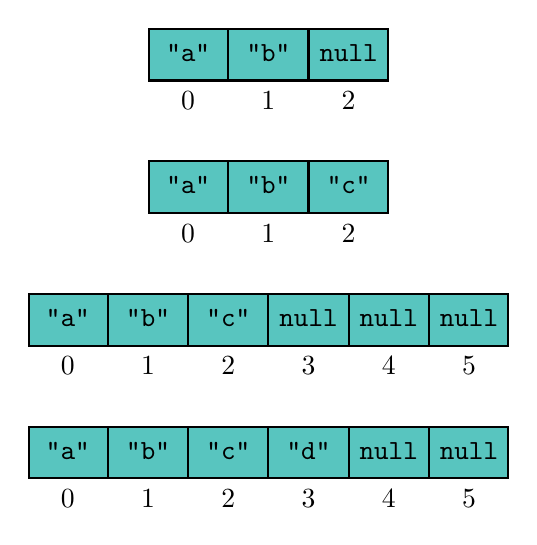
\begin{tikzpicture}[
  thick,
  myrect/.style={
    draw,
    fill=myseagreen,
    rectangle split,
    rectangle split horizontal,
    rectangle split parts=#1,
    rectangle split part align=left,
    text width=5ex,
    text centered
    },
  mycallout/.style={
    shape=rectangle callout,
    rounded corners,
    fill=mysalmon,
    callout absolute pointer={#1},
    callout pointer width=1cm
  }  
]

\node[myrect=3]
  (array1)
  {
  					\strut \texttt{"a"}
  \nodepart{two}	\strut \texttt{"b"}
  \nodepart{three}	\strut \texttt{null}
  };
\foreach \Valor [count=\Valori from 0] in {one ,two ,three }
  \node[below] at (array1.\Valor south) {\Valori};

\node[myrect=3]
  (array2)[below=of array1]
  {
  					\strut \texttt{"a"}
  \nodepart{two}	\strut \texttt{"b"}
  \nodepart{three}	\strut \texttt{"c"}
  };
\foreach \Valor [count=\Valori from 0] in {one ,two ,three }
  \node[below] at (array2.\Valor south) {\Valori};

\node[myrect=6]
  (array3)[below=of array2]
  {
  					\strut \texttt{"a"}
  \nodepart{two}	\strut \texttt{"b"}
  \nodepart{three}	\strut \texttt{"c"}
  \nodepart{four}	\strut \texttt{null}
  \nodepart{five}	\strut \texttt{null}
  \nodepart{six}	\strut \texttt{null}
  };
\foreach \Valor [count=\Valori from 0] in {one ,two ,three , four , five , six }
  \node[below] at (array3.\Valor south) {\Valori};

\node[myrect=6]
  (array4)[below=of array3]
  {
  					\strut \texttt{"a"}
  \nodepart{two}	\strut \texttt{"b"}
  \nodepart{three}	\strut \texttt{"c"}
  \nodepart{four}	\strut \texttt{"d"}
  \nodepart{five}	\strut \texttt{null}
  \nodepart{six}	\strut \texttt{null}
  };
\foreach \Valor [count=\Valori from 0] in {one ,two ,three , four , five , six }
  \node[below] at (array4.\Valor south) {\Valori};

\end{tikzpicture}
}
\end{center}

We see that there is still room in the array to add \texttt{"c"}, but to add more elements to the list, we must use a new array with double the length.

It's important to note that any given insertion to the structure is either $O(n)$ or $O(1)$, but there is only one $O(n)$ insertion for every $O(n)$ $O(1)$ insertions, so we still average out to constant time.

The Java implementation of a dynamic array is the \texttt{ArrayList}. The C++ implementation is the \texttt{vector}.

For the following operations, think about how you would implement each and analyze its time complexity. 

\begin{center}
  \begin{tabular}{ | p{5cm} | p{5cm} | p{5cm} | }
    \hline
    \textbf{Function}	&	\textbf{Java, \texttt{ArrayList}}	&	\textbf{C++, \texttt{vector}} \\ \hline
    \textit{add} an element to the end of the list		&	\texttt{boolean add(E e)}	&	\texttt{void push\_back(const value\_type\& val)}\footnote{\texttt{\& is a C++ reference}} \\ \hline
    \textit{insert} an element to a particular index in the list, shifting all subsequent elements down one index	&	\texttt{void add(int index, E element)}		&	\texttt{iterator insert(iterator position, const value\_type\& val)}\footnote{An \textit{iterator} is like a pointer that allows for traversal of a data structure in a particular order. For example, we can increment the iterator to access the next element in the list. An iterator is NOT merely an integer representing the relative position in our list, as the in the Java implementation of \texttt{add}}	\\ \hline
    \textit{access} the element stored at a particular index	&	\texttt{E get(int index)}		&	\texttt{reference operator[] (size\_type n)}\footnote{\texttt{size\_type} is, for our purposes, \texttt{unsigned int}, and \texttt{reference operator[]} makes this structure's syntax more like a normal array. In particular, to access the element at index \texttt{i} of a vector \texttt{v}, we simply use \texttt{v[i]}, and to update an element, we use \texttt{v[i] = val}.}	\\ \hline
    \textit{update} the value of the element stored at a particular index to a new element & \texttt{E set(int index, E element)} & \texttt{reference operator[] (size\_type n)} \\ \hline
    \textit{search} whether the list contains a particular element & \texttt{boolean contains(Object o)} & \texttt{iterator find (iterator first, iterator last, const value\_type\& val)}\footnote{This function is in \texttt{<algorithm>}.} \\ \hline
    \textit{remove} the element at a particular index from the list & \texttt{E remove(int index)} & \texttt{iterator erase (iterator position)} \\ \hline
    search for and \textit{remove} a given element from the list & \texttt{boolean remove(Object o)} & use iterators \\ \hline
    return the \textit{size} of the list\footnote{Note that the length of the list is not simply the size of the backing array.} & \texttt{int size()} & \texttt{size\_type size() const} \\ \hline
  \end{tabular}
\end{center}

Accessing and updating elements at particular indices are very nice. They are easy to code and run in constant time. These are the bread and butter of any array. Adding at the end of the list is nice as well. Checking whether some element is contained in the list is a pain, as it is $O(n)$, and adding to and removing from early in the list are more annoying.

\subsection{Linked List}

Arrays are nice for accessing, say, the seventh element in the list. We extend this to the dynamic array to implement adding and removing elements to and from the end of the list nicely. Removing elements from the beginning of the list, however, is cumbersome.

The \textit{linked list} attempts to remedy this. It trades $O(1)$ access to any element in the list for an easier way to remove elements from either end of the list easily. Consider a chain of paper clips:

\begin{center}

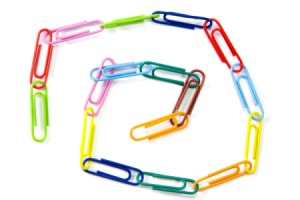
\includegraphics{images/paper_clip_chain.jpg}\footnote{\url{http://img.thrfun.com/img/078/156/paper_clip_chain_s1.jpg}}

\end{center}

It's easy to add or remove more paper clips from either end of the chain, and from any given paper clip, it's easy to access the paper clip directly previous or next to it in the chain. If we needed the seventh paper clip in the chain, we'd need to manually count, an $O(n)$ operation. However, if we then needed to remove that paper clip from the chain, it wouldn't be that hard, assuming we kept a finger, or pointer, on the seventh paper clip.

The best way to think about and implement a linked list is through a cyclical doubly-linked list, with a dummy head. This means each element has its own node container, while the head of the list is simply a node without an element. Such a data structure looks something like this:

\begin{center}


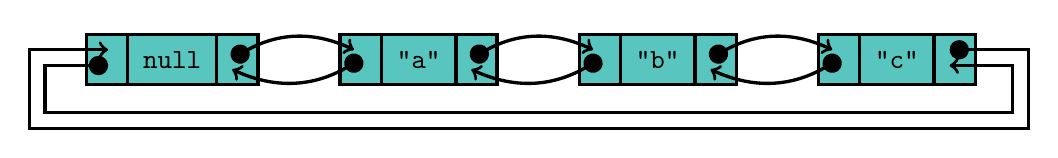
\begin{tikzpicture}[
        list/.style={
            very thick, rectangle split, 
            rectangle split parts=3, draw, 
            rectangle split horizontal, minimum size=18pt,
            inner sep=5pt, text=black,
            rectangle split part fill=myseagreen
        }, 
        ->, start chain, very thick
      ]

  \node[list,on chain] (dummy) {\nodepart{second} \texttt{null}};
  \node[list,on chain] (A) {\nodepart{second} \texttt{"a"}};
  \node[list,on chain] (B) {\nodepart{second} \texttt{"b"}};
  \node[list,on chain] (C) {\nodepart{second} \texttt{"c"}};

    \path[*->] let \p1 = (dummy.three), \p2 = (dummy.center) in (\x1,\y2) edge [bend left] ($(A.one)+(0,0.2)$);
  \path[*->] let \p1 = (A.three), \p2 = (A.center) in (\x1,\y2) edge [bend left] ($(B.one)+(0,0.2)$);
  \path[*->] let \p1 = (B.three), \p2 = (B.center) in (\x1,\y2) edge [bend left] ($(C.one)+(0,0.2)$);
  
%  \draw[*->] let \p1 = (C.three), \p2 = (C.center) in (\x1,\y2) -- (dummy);

%  \draw[*->] ($(A.one)+(0.2,0.1)$) -- (dummy);
  \path[*->] ($(B.one)+(0.1,0.1)$) edge [bend left] ($(A.three)+(0,-0.05)$);
  \path[*->] ($(C.one)+(0.1,0.1)$) edge [bend left] ($(B.three)+(0,-0.05)$);
    \path[*->] ($(A.one)+(0.1,0.1)$) edge [bend left] ($(dummy.three)+(0,-0.05)$);
    
    \draw[*->] ($(C.three)+(0.0,0.2)$) -- ($(C.three)+(1.0,0.2)$) -- ($(C.three)+(1.0,-0.8)$) -- ($(dummy.one)+(-0.9,-0.8)$) -- ($(dummy.one)+(-0.9,0.2)$) -- ($(dummy.one)+(0.1,0.2)$);

    \draw[<-*] ($(C.three)+(0.0,0.0)$) -- ($(C.three)+(0.8,0.0)$) -- ($(C.three)+(0.8,-0.6)$) -- ($(dummy.one)+(-0.7,-0.6)$) -- ($(dummy.one)+(-0.7,0.0)$) -- ($(dummy.one)+(0.1,0.0)$);

\end{tikzpicture}

\end{center}

We see that each node maintains a pointer to its next neighbor and its previous neighbor, in addition to containing the String it stores. We can store this data in a class like the following:

\begin{mylstlisting}
class ListNode<E> {
	ListNode prev, next;
    E s;
}
\end{mylstlisting}

If we were to insert an element after a ListNode \texttt{a}, it is necessary to update all pointers:

\begin{mylstlisting}
ListNode<String> b = new ListNode<String>();
b.prev = a;
b.next = a.next;
b.next.prev = b;
a.next = b;
\end{mylstlisting}

Since the linked list is symmetric, inserting an element before a node is also easy. To add something to the end of the list, simply add it before the dummy head. From here it should not be too hard to implement all the important functions of a linked list.

The Java implementation of a linked list is \texttt{LinkedList}, and the C++ implementation is \texttt{list}. A second C++ class that performs the same tasks but uses a backing array instead of a linked list structure is the \texttt{deque}.

\begin{center}
    \begin{tabular}{ | p{3cm} | p{4cm} | p{4cm} | p{4cm} | }
      \hline
      \textbf{Function}	&	\textbf{Java, \texttt{LinkedList}}	&	\textbf{C++, \texttt{list}} & \textbf{C++, \texttt{deque}} \\ \hline
      \textit{add} an element to the end & \texttt{boolean add(E e)} & \multicolumn{2}{p{8cm} |}{\centering \texttt{void push\_back(const value\_type\& val)}} \\ \hline
      \textit{insert}\footnote{The index in a linked list is implicit.} & \texttt{void add(int index, E element)} & \multicolumn{2}{p{8cm} |}{\centering \texttt{iterator insert(iterator position, const value\_type\& val)}} \\ \hline
      \textit{access} & \texttt{E get(int index)} & use iterators & \texttt{reference operator[] (size\_type n)} \\ \hline
      \textit{update} & \texttt{E set(int index, E element)} & use iterators & \texttt{reference operator[] (size\_type n)} \\ \hline
      \textit{search} & \texttt{boolean contains(Object o)} & \multicolumn{2}{p{8cm} |}{\centering \texttt{iterator find (iterator first, iterator last, const value\_type\& val)}\footnote{This function is in \texttt{<algorithm>}.}} \\ \hline
      \textit{remove} the element at a particular index & \texttt{E remove(int index)} & \multicolumn{2}{p{8cm} |}{\centering \texttt{iterator erase (iterator position)}} \\ \hline
      search for and \textit{remove} a given element & \texttt{boolean remove(Object o)} & \texttt{void remove (const value\_type\& val)} & use iterators \\ \hline
      \textit{size} & \texttt{int size()} & \multicolumn{2}{p{8cm} |}{\centering \texttt{size\_type size() const}} \\ \hline
      end operations & \texttt{addFirst}, \texttt{addLast}, \texttt{getFirst}, \texttt{getLast}, \texttt{removeFirst}, \texttt{removeLast} & \multicolumn{2}{p{8cm} |}{\texttt{push\_front}, \texttt{push\_back}, \texttt{pop\_front}, \texttt{pop\_back}} \\ \hline
    \end{tabular}
  \end{center}

With a linked list implemented, two other data structures immediately follow.

\section{Stack}

A \textit{stack} gets its name from being exactly that: a stack. If we have a stack of papers, we can push things on the top and pop things off the top. Sometimes we peek at to access the element on top but don't actually remove anything. We never do anything with what's on the bottom. This is called \textit{LIFO}: Last In, First Out.

Java implements the stack with \texttt{Stack}, C++ with \texttt{stack}.

\begin{center}
    \begin{tabular}{ | p{5cm} | p{5cm} | p{5cm} | }
      \hline
      \textbf{Function}	&	\textbf{Java, \texttt{Stack}}	&	\textbf{C++, \texttt{stack}} \\ \hline
      \textit{push}		&	\texttt{E push(E item)}	&	\texttt{void push (const value\_type\& val)} \\ \hline
      \textit{pop}			&	\texttt{E poll()}		&	\texttt{void pop()}	\\ \hline
      \textit{top}		&	\texttt{E peek()}		&	\texttt{value\_type\& top()}	\\ \hline
      \textit{size} & \texttt{int size()} & \texttt{size\_type size() const} \\ \hline
    \end{tabular}
\end{center}

Java implements \texttt{Stack} using an array-like structure. This works just as well, and is faster in practice, but I prefer the linked-list structure as a mathematical concept as it is more elegant in its relationship with the queue and more easily customizable.

\section{Queue}

A \textit{queue} is like a queue waiting in line for lunch. We push to the end and pop from the front. Sometimes we peek at the front but don't actually remove anything. The first person in line gets served first. This is called \textit{FIFO}: First In, First Out.

In Java, \texttt{Queue} is an interface, and in C++, the implementation of the queue is \texttt{queue}.

\begin{center}
  \begin{tabular}{ | p{5cm} | p{5cm} | p{5cm} | }
    \hline
    \textbf{Function}	&	\textbf{Java, \texttt{Queue}}	&	\textbf{C++, \texttt{queue}} \\ \hline
    \textit{push}		&	\texttt{boolean offer(E e)}	&	\texttt{void push (const value\_type\& val)} \\ \hline
    \textit{pop}			&	\texttt{E poll()}		&	\texttt{void pop()}	\\ \hline
    \textit{top}		&	\texttt{E peek()}		&	\texttt{value\_type\& front()}	\\ \hline
    \textit{size} & \texttt{int size()} & \texttt{size\_type size() const} \\ \hline
  \end{tabular}
\end{center}

Since \texttt{Queue} is an interface in Java, we cannot instantiate a \texttt{Queue}, so the following statement is illegal.

\begin{mylstlisting}
Queue<String> q = new Queue<String>();
\end{mylstlisting}

Instead, we must use \texttt{LinkedList}, so we do something like this:

\begin{mylstlisting}
Queue<String> q = new LinkedList<String>();
\end{mylstlisting}

This is legal because \texttt{LinkedList} implements \texttt{Queue}, making it the standard implementation of the FIFO queue.

\section{Heap}

Quite often a FIFO queue is not always desirable. For example, perhaps the string I want to remove at every given point is the one that is lexicographically least.

A min heap is a tree such that every node is smaller than or equal to all of its children. A max heap is a tree such that every node is larger than or equal to all of its children. Pictured is a complete binary min heap, which will be of use to us.

\begin{center}
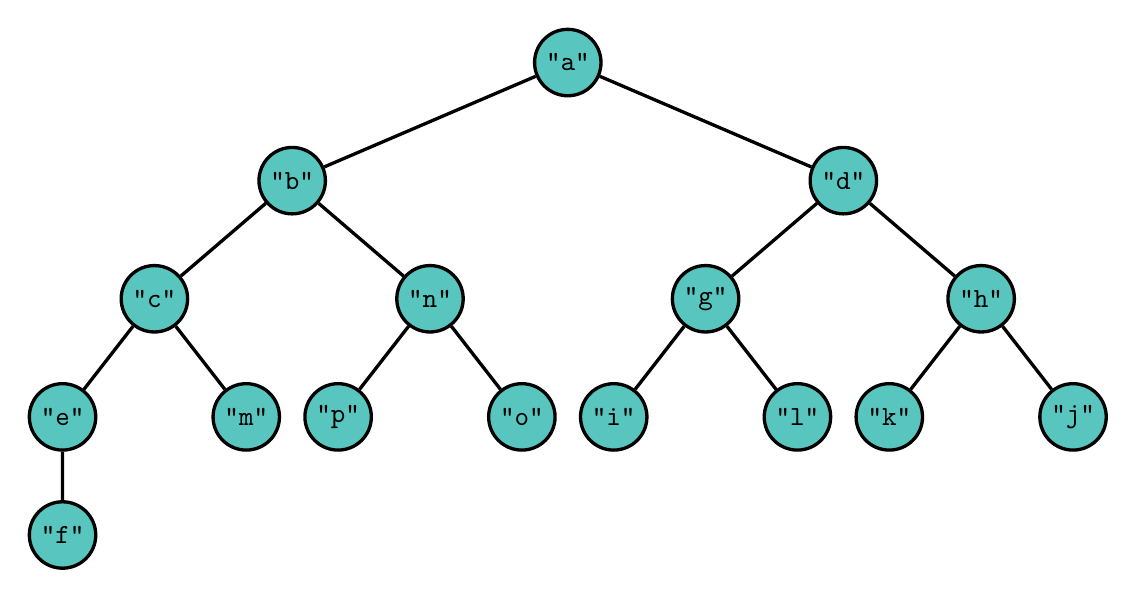
\begin{tikzpicture}[very thick,level/.style={sibling distance=70mm/#1}]
\node [vertex] (r){\texttt{"a"}}
  child {
    node [vertex] (a) {\texttt{"b"}}
    child {
      node [vertex] {\texttt{"c"}}
      child {
        node [vertex] {\texttt{"e"}}
        child {node [vertex] {\texttt{"f"}}}
      } 
      child {
        node [vertex] {\texttt{"m"}}
      }
    }
    child {
      node [vertex] {\texttt{"n"}}
      child {node [vertex] {\texttt{"p"}}}
      child {node [vertex] {\texttt{"o"}}}
    }
  }
  child {
    node [vertex] {\texttt{"d"}}
    child {
      node [vertex] {\texttt{"g"}}
      child {node [vertex] {\texttt{"i"}}}
      child {node [vertex] {\texttt{"l"}}}
    }
    child {
      node [vertex] {\texttt{"h"}}
      child {node [vertex] {\texttt{"k"}}}
      child {node [vertex] {\texttt{"j"}}}
    }
  };
\end{tikzpicture}
\end{center}

We see that the root of the tree will always be the smallest element. It is tempting to use a container class with a pointer to its left and its right child. However, we have a much nicer way to store \textit{complete} binary trees with an array. Consider the following numbering of the nodes:

\begin{center}
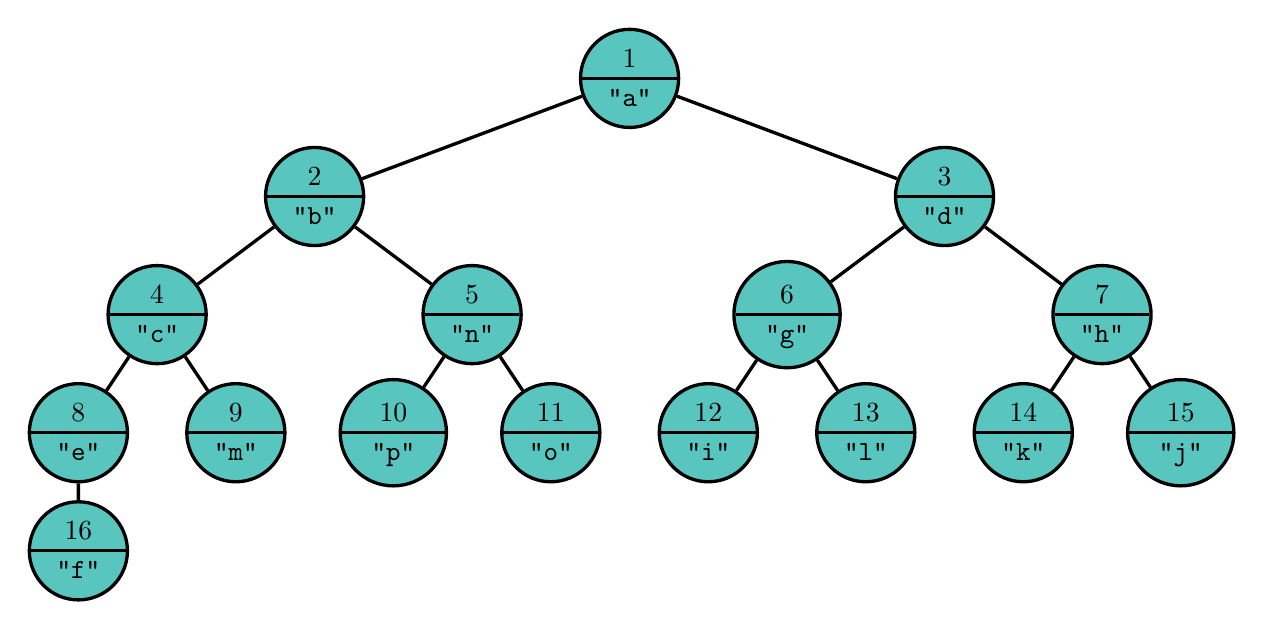
\begin{tikzpicture}[very thick,level 1/.style={sibling distance=80mm}, level 2/.style={sibling distance=40mm}, level 3/.style={sibling distance=20mm}]
\node [splitvertex] (r){1\nodepart{lower}\texttt{"a"}}
  child {
    node [splitvertex] (a) {2\nodepart{lower}\texttt{"b"}}
    child {
      node [splitvertex] {4\nodepart{lower}\texttt{"c"}}
      child {
        node [splitvertex] {8\nodepart{lower}\texttt{"e"}}
        child {node [splitvertex] {16\nodepart{lower}\texttt{"f"}}}
      } 
      child {
        node [splitvertex] {9\nodepart{lower}\texttt{"m"}}
      }
    }
    child {
      node [splitvertex] {5\nodepart{lower}\texttt{"n"}}
      child {node [splitvertex] {10\nodepart{lower}\texttt{"p"}}}
      child {node [splitvertex] {11\nodepart{lower}\texttt{"o"}}}
    }
  }
  child {
    node [splitvertex] {3\nodepart{lower}\texttt{"d"}}
    child {
      node [splitvertex] {6\nodepart{lower}\texttt{"g"}}
      child {node [splitvertex] {12\nodepart{lower}\texttt{"i"}}}
      child {node [splitvertex] {13\nodepart{lower}\texttt{"l"}}}
    }
    child {
      node [splitvertex] {7\nodepart{lower}\texttt{"h"}}
      child {node [splitvertex] {14\nodepart{lower}\texttt{"k"}}}
      child {node [splitvertex] {15\nodepart{lower}\texttt{"j"}}}
    }
  };
\end{tikzpicture}
\end{center}

We see that every number from 1 to 16 is used, and for every node, if the index associated with it is $i$, the left child is $2i$, and the right child is $2i+1$. This leads to a very natural implementation of the tree in an array:

\begin{center}
{
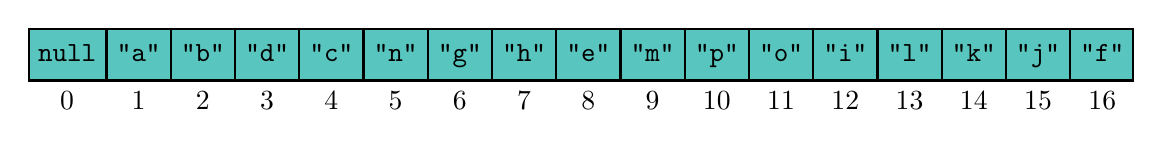
\begin{tikzpicture}[
  thick,
  myrect/.style={
    draw,
    fill=myseagreen,
    rectangle split,
    rectangle split horizontal,
    rectangle split parts=#1,
    rectangle split part align=left,
    text centered
    },
  mycallout/.style={
    shape=rectangle callout,
    rounded corners,
    fill=mysalmon,
    callout absolute pointer={#1},
    callout pointer width=1cm
  }  
]

\node[myrect=17]
  (array)
  {
  					\strut \texttt{null}
  \nodepart{two}	\strut \texttt{"a"}
  \nodepart{three}	\strut \texttt{"b"}
  \nodepart{four}	\strut \texttt{"d"}
  \nodepart{five}	\strut \texttt{"c"}
  \nodepart{six}	\strut \texttt{"n"}
  \nodepart{seven}	\strut \texttt{"g"}
  \nodepart{eight}	\strut \texttt{"h"}
  \nodepart{nine}	\strut \texttt{"e"}
  \nodepart{ten}	\strut \texttt{"m"}
  \nodepart{eleven}	\strut \texttt{"p"}
  \nodepart{twelve}	\strut \texttt{"o"}
  \nodepart{thirteen}	\strut \texttt{"i"}
  \nodepart{fourteen}	\strut \texttt{"l"}
  \nodepart{fifteen}	\strut \texttt{"k"}
  \nodepart{sixteen}	\strut \texttt{"j"}
  \nodepart{seventeen}	\strut \texttt{"f"}
  };
\foreach \Valor [count=\Valori from 0] in {one ,two ,three ,four ,five ,six ,seven ,eight ,nine ,ten ,eleven ,twelve ,thirteen ,fourteen ,fifteen ,sixteen ,seventeen }
  \node[below] at (array.\Valor south) {\Valori};

\end{tikzpicture}
}
\end{center}

How do we add elements to our heap, while maintaining the heap qualities? Well, let's just add it to the very end and see what we get. Suppose we are to add \texttt{"b"} to the tree.

\begin{center}
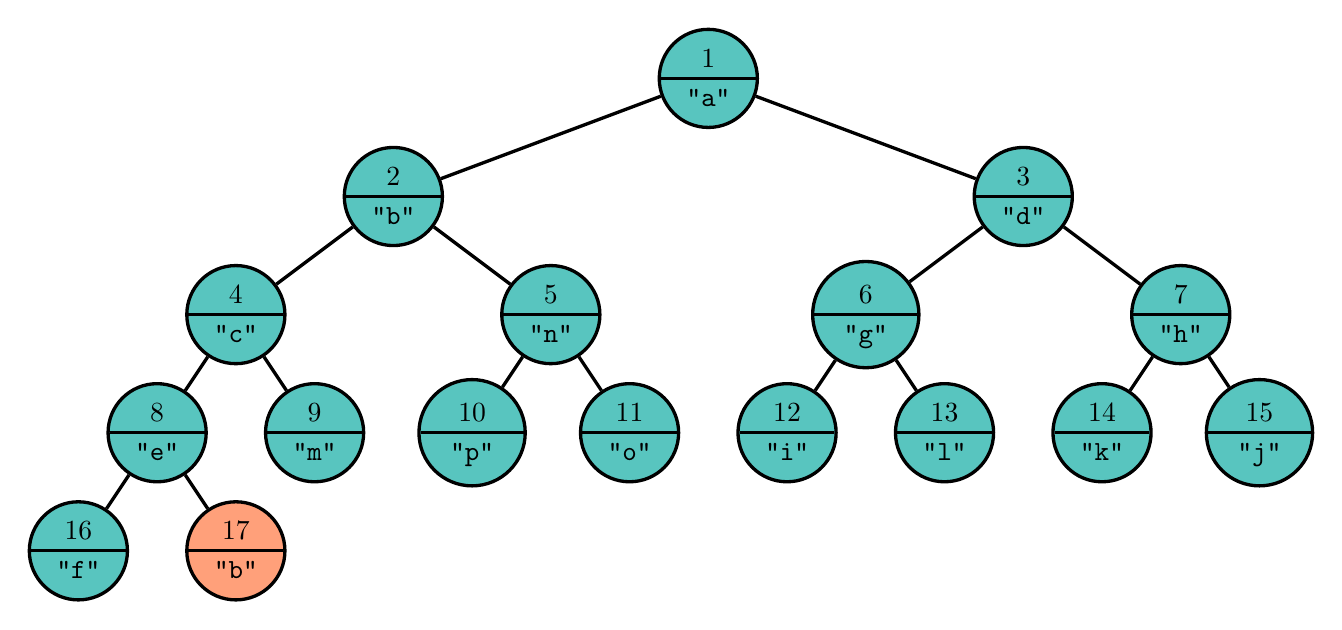
\begin{tikzpicture}[very thick,level 1/.style={sibling distance=80mm}, level 2/.style={sibling distance=40mm}, level 3/.style={sibling distance=20mm}]
\node [splitvertex] (r){1\nodepart{lower}\texttt{"a"}}
  child {
    node [splitvertex] (a) {2\nodepart{lower}\texttt{"b"}}
    child {
      node [splitvertex] {4\nodepart{lower}\texttt{"c"}}
      child {
        node [splitvertex] {8\nodepart{lower}\texttt{"e"}}
        child {node [splitvertex] {16\nodepart{lower}\texttt{"f"}}}
        child {node [splitvertex, fill=mysalmon] {17\nodepart{lower}\texttt{"b"}}}
      } 
      child {
        node [splitvertex] {9\nodepart{lower}\texttt{"m"}}
      }
    }
    child {
      node [splitvertex] {5\nodepart{lower}\texttt{"n"}}
      child {node [splitvertex] {10\nodepart{lower}\texttt{"p"}}}
      child {node [splitvertex] {11\nodepart{lower}\texttt{"o"}}}
    }
  }
  child {
    node [splitvertex] {3\nodepart{lower}\texttt{"d"}}
    child {
      node [splitvertex] {6\nodepart{lower}\texttt{"g"}}
      child {node [splitvertex] {12\nodepart{lower}\texttt{"i"}}}
      child {node [splitvertex] {13\nodepart{lower}\texttt{"l"}}}
    }
    child {
      node [splitvertex] {7\nodepart{lower}\texttt{"h"}}
      child {node [splitvertex] {14\nodepart{lower}\texttt{"k"}}}
      child {node [splitvertex] {15\nodepart{lower}\texttt{"j"}}}
    }
  };
\end{tikzpicture}
\end{center}

Well, \texttt{"b"} comes before \texttt{"e"} in the alphabet, so let's swap the nodes. We are guaranteed that \texttt{"b"} should come before the other child (in this case, \texttt{"f"}) by the transitive property.

\begin{center}
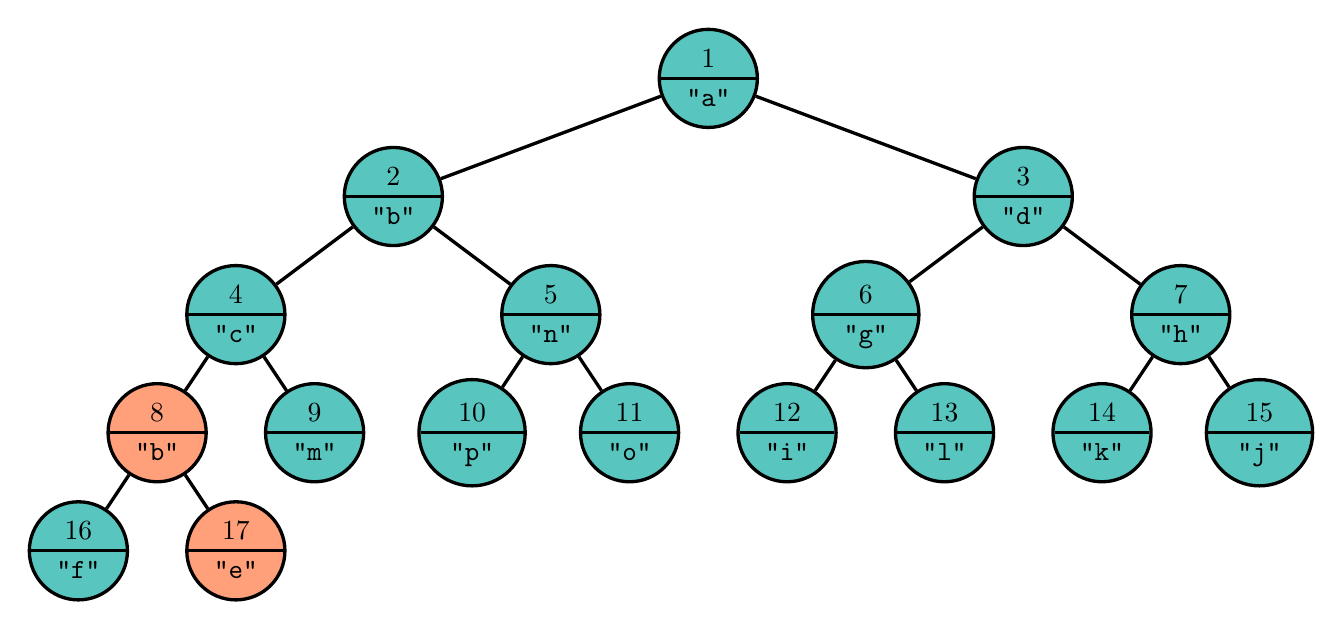
\begin{tikzpicture}[very thick,level 1/.style={sibling distance=80mm}, level 2/.style={sibling distance=40mm}, level 3/.style={sibling distance=20mm}]
\node [splitvertex] (r){1\nodepart{lower}\texttt{"a"}}
  child {
    node [splitvertex] (a) {2\nodepart{lower}\texttt{"b"}}
    child {
      node [splitvertex] {4\nodepart{lower}\texttt{"c"}}
      child {
        node [splitvertex, fill=mysalmon] {8\nodepart{lower}\texttt{"b"}}
        child {node [splitvertex] {16\nodepart{lower}\texttt{"f"}}}
        child {node [splitvertex, fill=mysalmon] {17\nodepart{lower}\texttt{"e"}}}
      } 
      child {
        node [splitvertex] {9\nodepart{lower}\texttt{"m"}}
      }
    }
    child {
      node [splitvertex] {5\nodepart{lower}\texttt{"n"}}
      child {node [splitvertex] {10\nodepart{lower}\texttt{"p"}}}
      child {node [splitvertex] {11\nodepart{lower}\texttt{"o"}}}
    }
  }
  child {
    node [splitvertex] {3\nodepart{lower}\texttt{"d"}}
    child {
      node [splitvertex] {6\nodepart{lower}\texttt{"g"}}
      child {node [splitvertex] {12\nodepart{lower}\texttt{"i"}}}
      child {node [splitvertex] {13\nodepart{lower}\texttt{"l"}}}
    }
    child {
      node [splitvertex] {7\nodepart{lower}\texttt{"h"}}
      child {node [splitvertex] {14\nodepart{lower}\texttt{"k"}}}
      child {node [splitvertex] {15\nodepart{lower}\texttt{"j"}}}
    }
  };
\end{tikzpicture}
\end{center}

One more swap...

\begin{center}
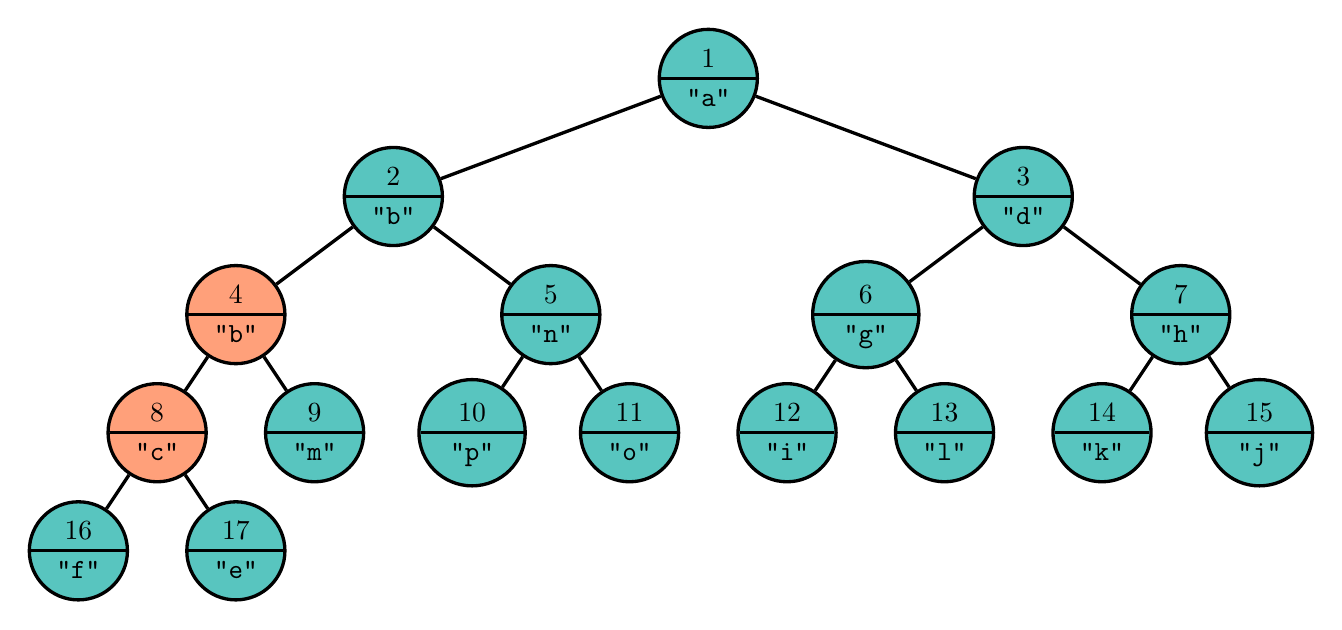
\begin{tikzpicture}[very thick,level 1/.style={sibling distance=80mm}, level 2/.style={sibling distance=40mm}, level 3/.style={sibling distance=20mm}]
\node [splitvertex] (r){1\nodepart{lower}\texttt{"a"}}
  child {
    node [splitvertex] (a) {2\nodepart{lower}\texttt{"b"}}
    child {
      node [splitvertex, fill=mysalmon] {4\nodepart{lower}\texttt{"b"}}
      child {
        node [splitvertex, fill=mysalmon] {8\nodepart{lower}\texttt{"c"}}
        child {node [splitvertex] {16\nodepart{lower}\texttt{"f"}}}
        child {node [splitvertex] {17\nodepart{lower}\texttt{"e"}}}
      } 
      child {
        node [splitvertex] {9\nodepart{lower}\texttt{"m"}}
      }
    }
    child {
      node [splitvertex] {5\nodepart{lower}\texttt{"n"}}
      child {node [splitvertex] {10\nodepart{lower}\texttt{"p"}}}
      child {node [splitvertex] {11\nodepart{lower}\texttt{"o"}}}
    }
  }
  child {
    node [splitvertex] {3\nodepart{lower}\texttt{"d"}}
    child {
      node [splitvertex] {6\nodepart{lower}\texttt{"g"}}
      child {node [splitvertex] {12\nodepart{lower}\texttt{"i"}}}
      child {node [splitvertex] {13\nodepart{lower}\texttt{"l"}}}
    }
    child {
      node [splitvertex] {7\nodepart{lower}\texttt{"h"}}
      child {node [splitvertex] {14\nodepart{lower}\texttt{"k"}}}
      child {node [splitvertex] {15\nodepart{lower}\texttt{"j"}}}
    }
  };
\end{tikzpicture}
\end{center}

And now we have the heap property restored. As the tree has depth at most $\log{n}$, this process is $O(\log{n})$.

To remove the root from the heap, we replace the root with the last leaf:

\begin{center}
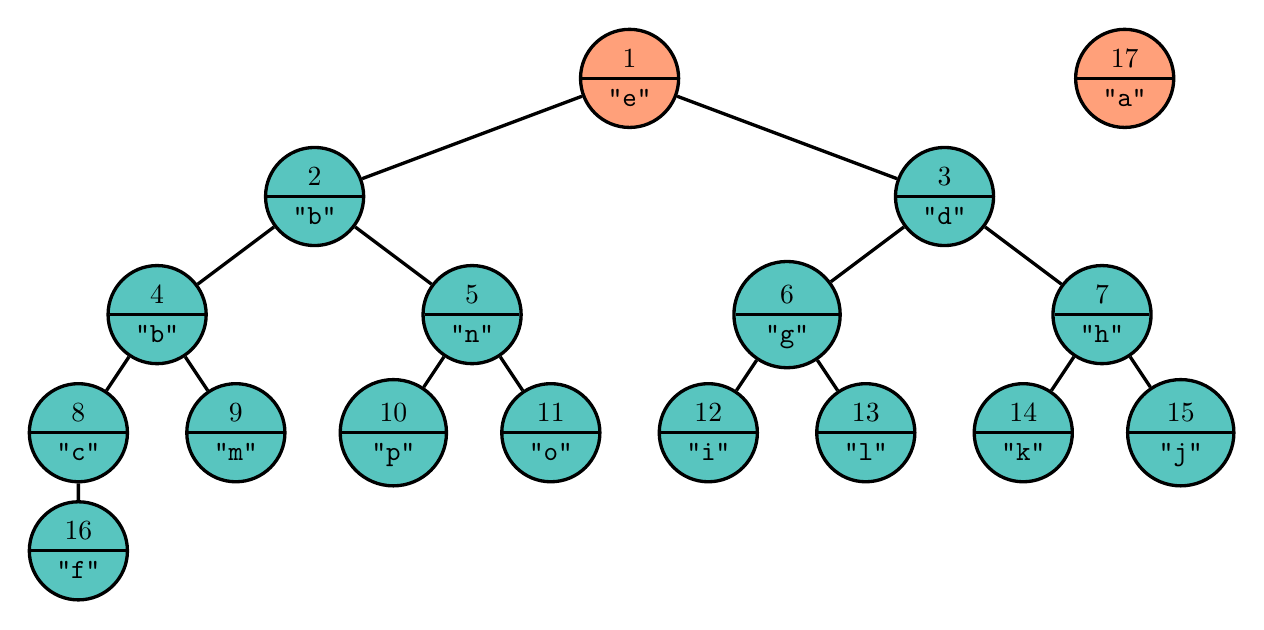
\begin{tikzpicture}[very thick,level 1/.style={sibling distance=80mm}, level 2/.style={sibling distance=40mm}, level 3/.style={sibling distance=20mm}]
\node [splitvertex, fill=mysalmon] (r){1\nodepart{lower}\texttt{"e"}}
  child {
    node [splitvertex] (a) {2\nodepart{lower}\texttt{"b"}}
    child {
      node [splitvertex] {4\nodepart{lower}\texttt{"b"}}
      child {
        node [splitvertex] {8\nodepart{lower}\texttt{"c"}}
        child {node [splitvertex] {16\nodepart{lower}\texttt{"f"}}}
      } 
      child {
        node [splitvertex] {9\nodepart{lower}\texttt{"m"}}
      }
    }
    child {
      node [splitvertex] {5\nodepart{lower}\texttt{"n"}}
      child {node [splitvertex] {10\nodepart{lower}\texttt{"p"}}}
      child {node [splitvertex] {11\nodepart{lower}\texttt{"o"}}}
    }
  }
  child {
    node [splitvertex] {3\nodepart{lower}\texttt{"d"}}
    child {
      node [splitvertex] {6\nodepart{lower}\texttt{"g"}}
      child {node [splitvertex] {12\nodepart{lower}\texttt{"i"}}}
      child {node [splitvertex] {13\nodepart{lower}\texttt{"l"}}}
    }
    child {
      node [splitvertex] {7\nodepart{lower}\texttt{"h"}}
      child {node [splitvertex] {14\nodepart{lower}\texttt{"k"}}}
      child {node [splitvertex] {15\nodepart{lower}\texttt{"j"}}}
    }
  };
  \node [splitvertex, fill=mysalmon] [right=5cm of r]{17\nodepart{lower}\texttt{"a"}};
\end{tikzpicture}
\end{center}

We perform a series of swaps to restore the heap property. We always want to choose the smaller child to swap until the heap property is satisfied.

\begin{center}
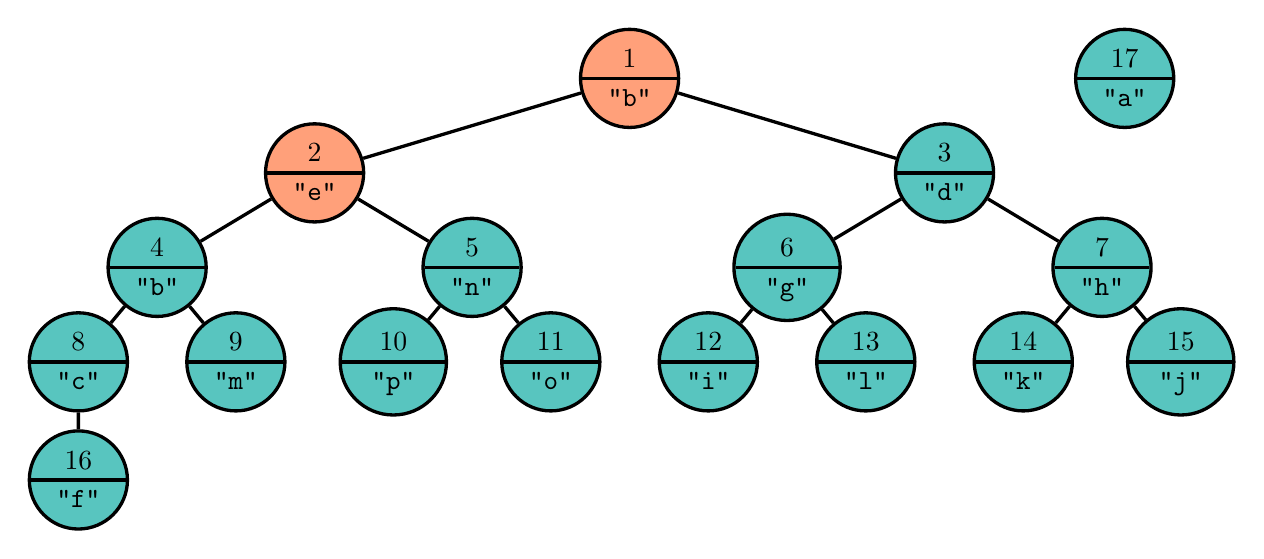
\begin{tikzpicture}[very thick,level 1/.style={sibling distance=80mm}, level 2/.style={sibling distance=40mm}, level 3/.style={sibling distance=20mm}, level distance=12mm, level 4/.style={level distance=15mm}]
\node [splitvertex, fill=mysalmon] (r){1\nodepart{lower}\texttt{"b"}}
  child {
    node [splitvertex, fill=mysalmon] (a) {2\nodepart{lower}\texttt{"e"}}
    child {
      node [splitvertex] {4\nodepart{lower}\texttt{"b"}}
      child {
        node [splitvertex] {8\nodepart{lower}\texttt{"c"}}
        child {node [splitvertex] {16\nodepart{lower}\texttt{"f"}}}
      } 
      child {
        node [splitvertex] {9\nodepart{lower}\texttt{"m"}}
      }
    }
    child {
      node [splitvertex] {5\nodepart{lower}\texttt{"n"}}
      child {node [splitvertex] {10\nodepart{lower}\texttt{"p"}}}
      child {node [splitvertex] {11\nodepart{lower}\texttt{"o"}}}
    }
  }
  child {
    node [splitvertex] {3\nodepart{lower}\texttt{"d"}}
    child {
      node [splitvertex] {6\nodepart{lower}\texttt{"g"}}
      child {node [splitvertex] {12\nodepart{lower}\texttt{"i"}}}
      child {node [splitvertex] {13\nodepart{lower}\texttt{"l"}}}
    }
    child {
      node [splitvertex] {7\nodepart{lower}\texttt{"h"}}
      child {node [splitvertex] {14\nodepart{lower}\texttt{"k"}}}
      child {node [splitvertex] {15\nodepart{lower}\texttt{"j"}}}
    }
  };
  \node [splitvertex] [right=5cm of r]{17\nodepart{lower}\texttt{"a"}};
\end{tikzpicture}
\end{center}

\begin{center}
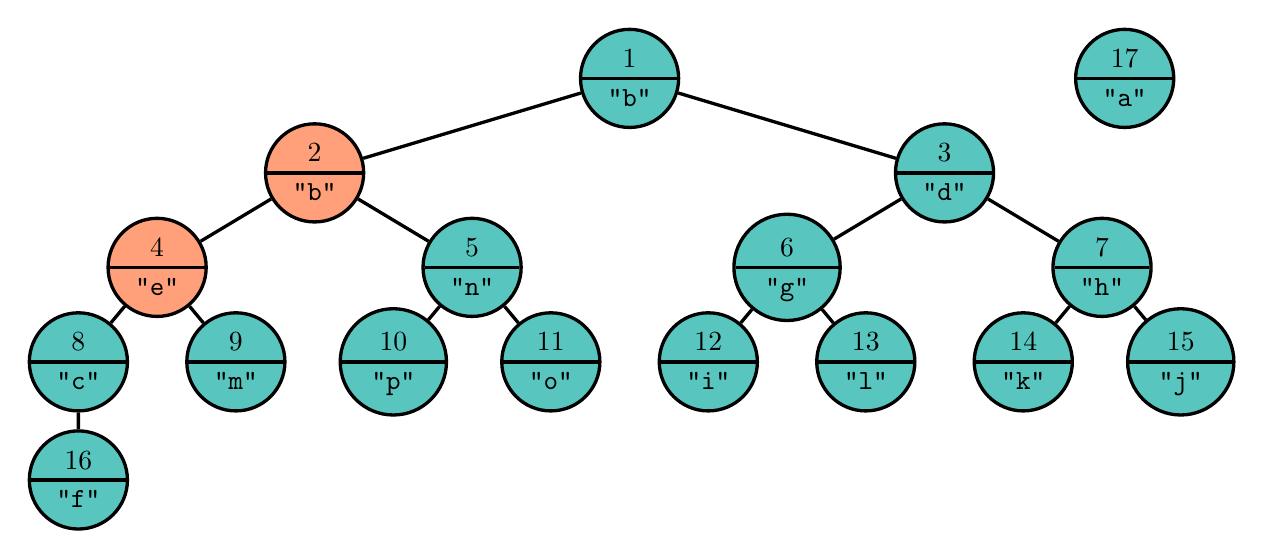
\begin{tikzpicture}[very thick,level 1/.style={sibling distance=80mm}, level 2/.style={sibling distance=40mm}, level 3/.style={sibling distance=20mm}, level distance=12mm, level 4/.style={level distance=15mm}]
\node [splitvertex] (r){1\nodepart{lower}\texttt{"b"}}
  child {
    node [splitvertex, fill=mysalmon] (a) {2\nodepart{lower}\texttt{"b"}}
    child {
      node [splitvertex, fill=mysalmon] {4\nodepart{lower}\texttt{"e"}}
      child {
        node [splitvertex] {8\nodepart{lower}\texttt{"c"}}
        child {node [splitvertex] {16\nodepart{lower}\texttt{"f"}}}
      } 
      child {
        node [splitvertex] {9\nodepart{lower}\texttt{"m"}}
      }
    }
    child {
      node [splitvertex] {5\nodepart{lower}\texttt{"n"}}
      child {node [splitvertex] {10\nodepart{lower}\texttt{"p"}}}
      child {node [splitvertex] {11\nodepart{lower}\texttt{"o"}}}
    }
  }
  child {
    node [splitvertex] {3\nodepart{lower}\texttt{"d"}}
    child {
      node [splitvertex] {6\nodepart{lower}\texttt{"g"}}
      child {node [splitvertex] {12\nodepart{lower}\texttt{"i"}}}
      child {node [splitvertex] {13\nodepart{lower}\texttt{"l"}}}
    }
    child {
      node [splitvertex] {7\nodepart{lower}\texttt{"h"}}
      child {node [splitvertex] {14\nodepart{lower}\texttt{"k"}}}
      child {node [splitvertex] {15\nodepart{lower}\texttt{"j"}}}
    }
  };
  \node [splitvertex] [right=5cm of r]{17\nodepart{lower}\texttt{"a"}};
\end{tikzpicture}
\end{center}

\begin{center}
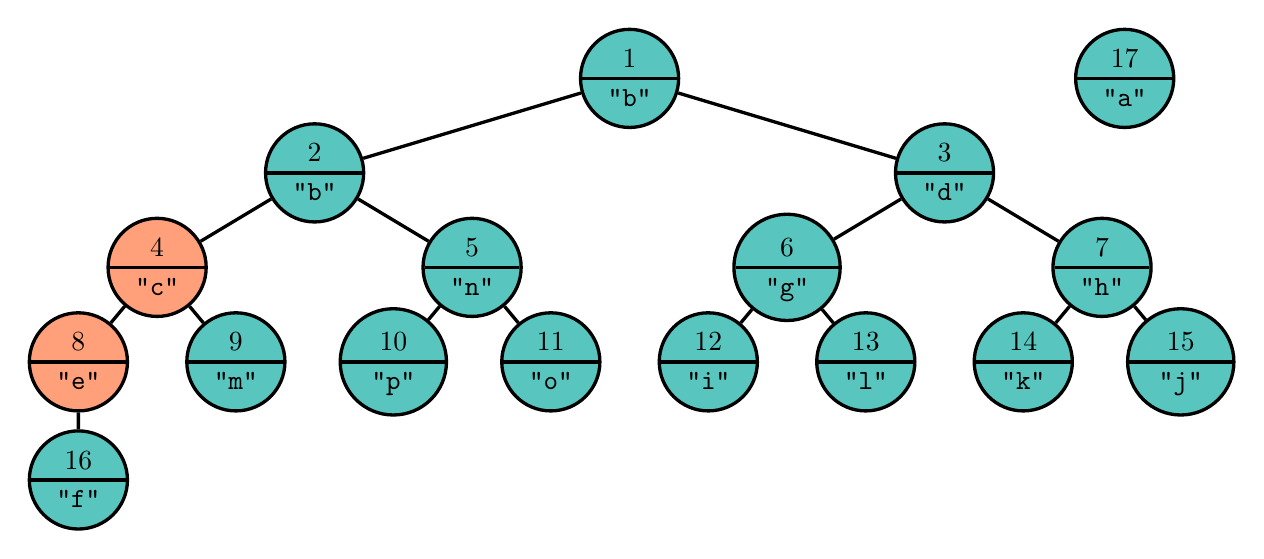
\begin{tikzpicture}[very thick,level 1/.style={sibling distance=80mm}, level 2/.style={sibling distance=40mm}, level 3/.style={sibling distance=20mm}, level distance=12mm, level 4/.style={level distance=15mm}]
\node [splitvertex] (r){1\nodepart{lower}\texttt{"b"}}
  child {
    node [splitvertex] (a) {2\nodepart{lower}\texttt{"b"}}
    child {
      node [splitvertex, fill=mysalmon] {4\nodepart{lower}\texttt{"c"}}
      child {
        node [splitvertex, fill=mysalmon] {8\nodepart{lower}\texttt{"e"}}
        child {node [splitvertex] {16\nodepart{lower}\texttt{"f"}}}
      } 
      child {
        node [splitvertex] {9\nodepart{lower}\texttt{"m"}}
      }
    }
    child {
      node [splitvertex] {5\nodepart{lower}\texttt{"n"}}
      child {node [splitvertex] {10\nodepart{lower}\texttt{"p"}}}
      child {node [splitvertex] {11\nodepart{lower}\texttt{"o"}}}
    }
  }
  child {
    node [splitvertex] {3\nodepart{lower}\texttt{"d"}}
    child {
      node [splitvertex] {6\nodepart{lower}\texttt{"g"}}
      child {node [splitvertex] {12\nodepart{lower}\texttt{"i"}}}
      child {node [splitvertex] {13\nodepart{lower}\texttt{"l"}}}
    }
    child {
      node [splitvertex] {7\nodepart{lower}\texttt{"h"}}
      child {node [splitvertex] {14\nodepart{lower}\texttt{"k"}}}
      child {node [splitvertex] {15\nodepart{lower}\texttt{"j"}}}
    }
  };
  \node [splitvertex] [right=5cm of r]{17\nodepart{lower}\texttt{"a"}};
\end{tikzpicture}
\end{center}

And we are done. Once again, this takes at most $\log(N)$ swaps. This idea can be extended to removing or changing the value of any node we'd like from a tree -- this is particularly useful for Dijkstra later.

Remember to implement your heap in an array-like structure!

Java implements a min heap with the \texttt{PriorityQueue}. This class, like \texttt{LinkedList}, also implements \texttt{Queue}. C++ implements a \textit{max}\footnote{Don't forget that C++ implements a max heap, ever.} heap with the \texttt{priority\_queue}. The functions for heaps in both languages are nearly identical to those for queues.

\begin{center}
    \begin{tabular}{ | p{5cm} | p{5cm} | p{5cm} | }
      \hline
      \textbf{Function}	&	\textbf{Java, \texttt{PriorityQueue}}	&	\textbf{C++, \texttt{priority\_queue}} \\ \hline
      \textit{push}		&	\texttt{boolean offer(E e)}	&	\texttt{void push (const value\_type\& val)} \\ \hline
      \textit{pop}			&	\texttt{E poll()}		&	\texttt{void pop()}	\\ \hline
      \textit{top}		&	\texttt{E peek()}		&	\texttt{value\_type\& top()}	\\ \hline
      \textit{size} & \texttt{int size()} & \texttt{size\_type size() const} \\ \hline
    \end{tabular}
\end{center}

\section{Set}

A \textit{set} is a collection of objects with no duplicate elements. Note that the data structures discussed in this section can be extended to become multisets, but Java and C++ implementations of these explicitly disallow multiplicity.

\subsection{Binary Search Tree}

A \textit{binary search tree (BST)} is a tree where every node is greater than every node in its left subtree and less than every node in its right subtree. As with a heap, to use a BST, we need to impose some kind of ordering on the elements stored.

\begin{center}
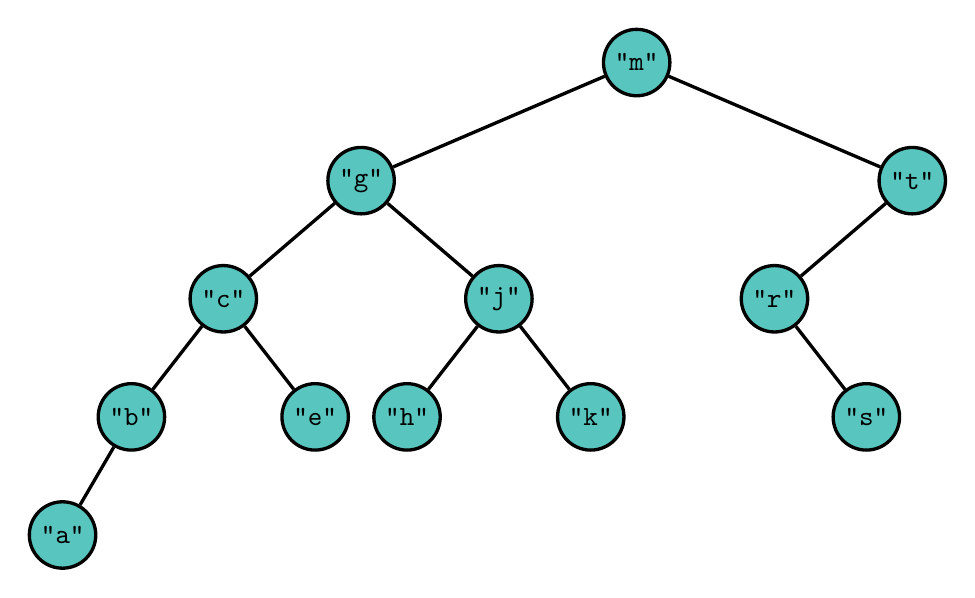
\begin{tikzpicture}[very thick,level/.style={sibling distance=70mm/#1}]
\node [vertex] (r){\texttt{"m"}}
  child {
    node [vertex] {\texttt{"g"}}
    child {
      node [vertex] {\texttt{"c"}}
      child {
        node [vertex] {\texttt{"b"}}
        child {node [vertex] {\texttt{"a"}}}
        child[missing]
      } 
      child {
        node [vertex] {\texttt{"e"}}
      }
    }
    child {
      node [vertex] {\texttt{"j"}}
      child {node [vertex] {\texttt{"h"}}}
      child {node [vertex] {\texttt{"k"}}}
    }
  }
  child {
    node [vertex] {\texttt{"t"}}
    child {
      node [vertex] {\texttt{"r"}}
      child[missing]
      child {node [vertex] {\texttt{"s"}}}
    }
    child[missing]
  };
\end{tikzpicture}
\end{center}

The tree need not be complete, unlike the heap. Because it is not guaranteed to be complete, there is no way to nicely bound the size of the array we would need if we were to use the same storage method as with the heap. Thus, we are forced to use a \texttt{TreeNode}, with left and right pointers. This is also problematic when determining guarantees on time complexities later, but the ways to solve this problem are pretty complicated so we'll ignore them for now.

Given the name of the tree, searching for an element within the tree is quite natural, and similar to a binary search. Compare the element to be searched for with the current node. If they are equal, we are done; otherwise, search the appropriate left or right subtree. As with most structures and algorithms with a binary search structure, this operation lends itself nicely to recursion. If the tree is reasonably nice, we expect to complete this in $O(\log{n})$ time, but searching can be as bad as linear if the tree looks like a linked list.

Adding an element is also natural. As our tree represents a set, it will not contain the same element twice. We trace down until we hit a null pointer, and add the element in the appropriate spot. Let's add a \texttt{"p"} to the BST:

\begin{center}
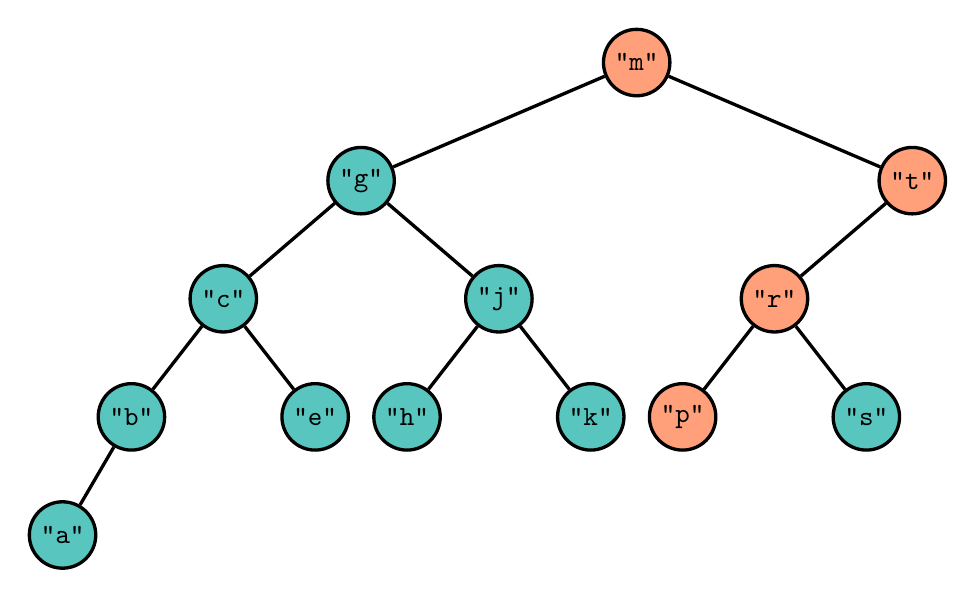
\begin{tikzpicture}[very thick,level/.style={sibling distance=70mm/#1}]
\node [vertex, fill=mysalmon] (r){\texttt{"m"}}
  child {
    node [vertex] {\texttt{"g"}}
    child {
      node [vertex] {\texttt{"c"}}
      child {
        node [vertex] {\texttt{"b"}}
        child {node [vertex] {\texttt{"a"}}}
        child[missing]
      } 
      child {
        node [vertex] {\texttt{"e"}}
      }
    }
    child {
      node [vertex] {\texttt{"j"}}
      child {node [vertex] {\texttt{"h"}}}
      child {node [vertex] {\texttt{"k"}}}
    }
  }
  child {
    node [vertex, fill=mysalmon] {\texttt{"t"}}
    child {
      node [vertex, fill=mysalmon] {\texttt{"r"}}
      child {node [vertex, fill=mysalmon] {\texttt{"p"}}}
      child {node [vertex] {\texttt{"s"}}}
    }
    child[missing]
  };
\end{tikzpicture}
\end{center}

Deleting an element is the annoying part. Unfortunately, there's not much we can do besides casework.

Removing a leaf, like \texttt{"a"}, from the tree is very easy. Removing a node with only once child, like \texttt{"t"}, is also relatively straightforward.

\begin{center}
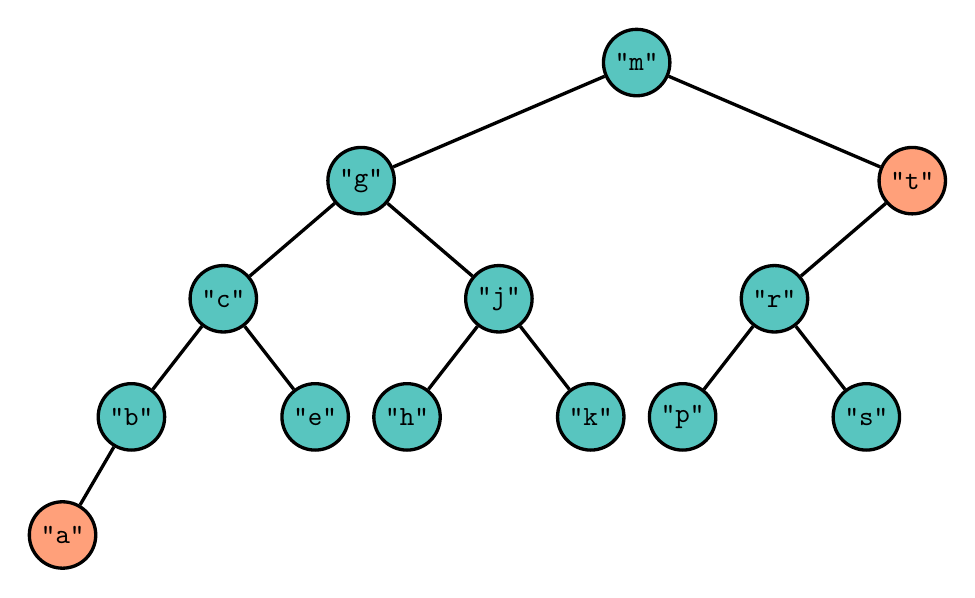
\begin{tikzpicture}[very thick,level/.style={sibling distance=70mm/#1}]
\node [vertex] (r){\texttt{"m"}}
  child {
    node [vertex] {\texttt{"g"}}
    child {
      node [vertex] {\texttt{"c"}}
      child {
        node [vertex] {\texttt{"b"}}
        child {node [vertex,fill=mysalmon] {\texttt{"a"}}}
        child[missing]
      } 
      child {
        node [vertex] {\texttt{"e"}}
      }
    }
    child {
      node [vertex] {\texttt{"j"}}
      child {node [vertex] {\texttt{"h"}}}
      child {node [vertex] {\texttt{"k"}}}
    }
  }
  child {
    node [vertex, fill=mysalmon] {\texttt{"t"}}
    child {
      node [vertex] {\texttt{"r"}}
      child {node [vertex] {\texttt{"p"}}}
      child {node [vertex] {\texttt{"s"}}}
    }
    child[missing]
  };
\end{tikzpicture}
\end{center}

Now, removing an element with two children is tricky. We'll try to remove \texttt{"g"}. Consider the least element in the right subtree of \texttt{"g"}, which in this case is \texttt{"h"}. We find \texttt{"h"} by always choosing the left child on the right subtree until we cannot go any further. This must be the least element.

\begin{center}
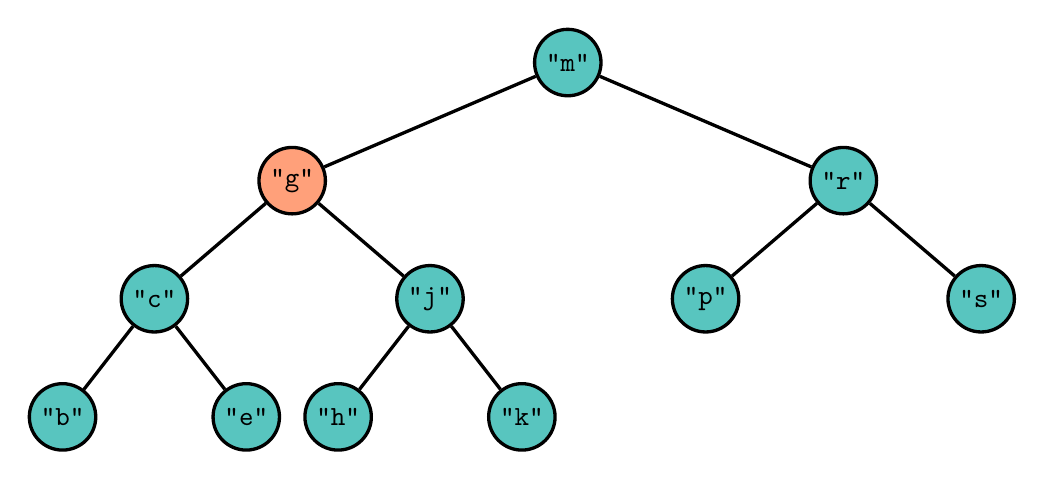
\begin{tikzpicture}[very thick,level/.style={sibling distance=70mm/#1}]
\node [vertex] (r){\texttt{"m"}}
  child {
    node [vertex, fill=mysalmon] {\texttt{"g"}}
    child {
      node [vertex] {\texttt{"c"}}
      child {
        node [vertex] {\texttt{"b"}}
      } 
      child {
        node [vertex] {\texttt{"e"}}
      }
    }
    child {
      node [vertex] {\texttt{"j"}}
      child {node [vertex] {\texttt{"h"}}}
      child {node [vertex] {\texttt{"k"}}}
    }
  }
  child {
      node [vertex] {\texttt{"r"}}
      child {node [vertex] {\texttt{"p"}}}
      child {node [vertex] {\texttt{"s"}}}
  };
\end{tikzpicture}
\end{center}

Note that \texttt{"h"} has either no children or only one child, and that nodes like these are easy to remove. We then change the value of the node containing \texttt{"g"} to \texttt{"h"}, which is legal since \texttt{"h"} is the least element, and remove \texttt{"h"} from the right subtree, and we are done.

\begin{center}
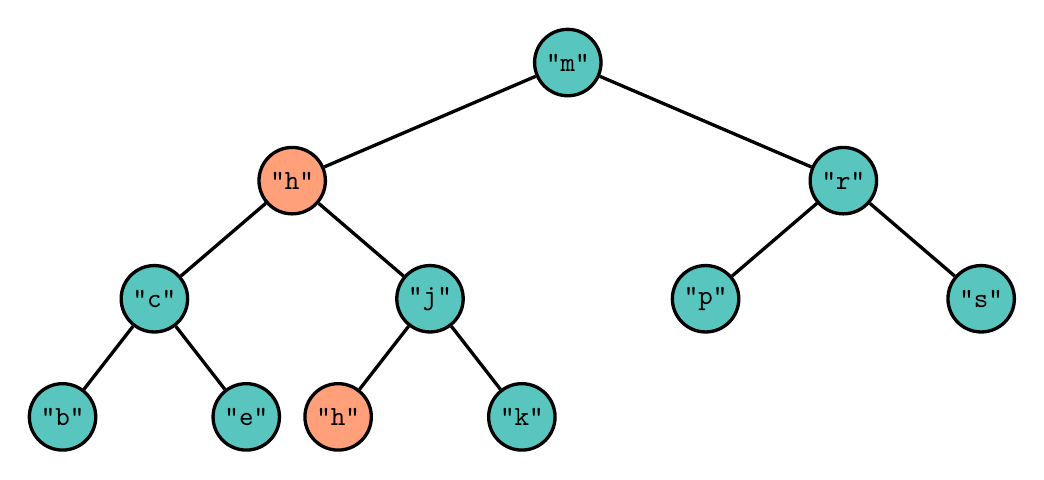
\begin{tikzpicture}[very thick,level/.style={sibling distance=70mm/#1}]
\node [vertex] (r){\texttt{"m"}}
  child {
    node [vertex, fill=mysalmon] {\texttt{"h"}}
    child {
      node [vertex] {\texttt{"c"}}
      child {
        node [vertex] {\texttt{"b"}}
      } 
      child {
        node [vertex] {\texttt{"e"}}
      }
    }
    child {
      node [vertex] {\texttt{"j"}}
      child {node [vertex, fill=mysalmon] {\texttt{"h"}}}
      child {node [vertex] {\texttt{"k"}}}
    }
  }
  child {
      node [vertex] {\texttt{"r"}}
      child {node [vertex] {\texttt{"p"}}}
      child {node [vertex] {\texttt{"s"}}}
  };
\end{tikzpicture}
\end{center}

\begin{center}
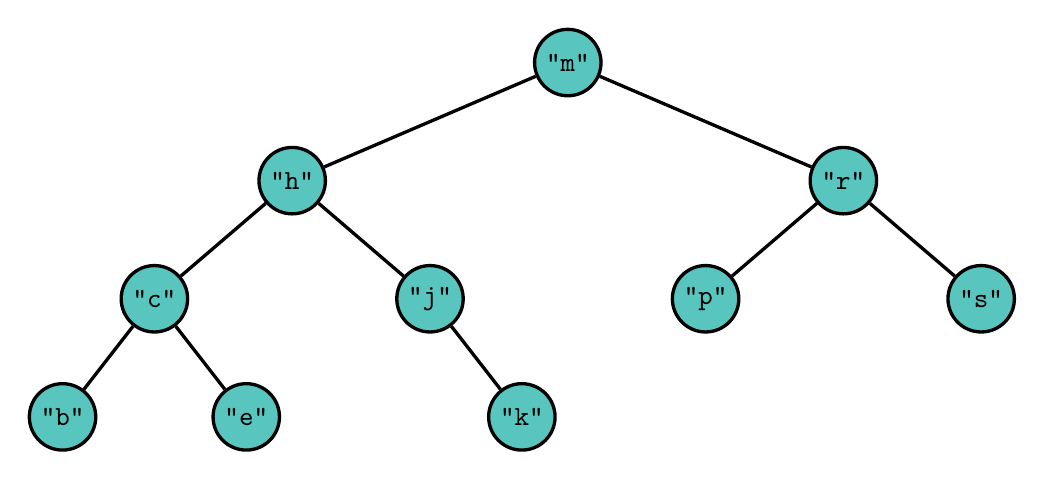
\begin{tikzpicture}[very thick,level/.style={sibling distance=70mm/#1}]
\node [vertex] (r){\texttt{"m"}}
  child {
    node [vertex] {\texttt{"h"}}
    child {
      node [vertex] {\texttt{"c"}}
      child {
        node [vertex] {\texttt{"b"}}
      } 
      child {
        node [vertex] {\texttt{"e"}}
      }
    }
      child {node [vertex] {\texttt{"j"}}
      	child[missing]
        child {
        	node[vertex]{\texttt{"k"}}
        }
      }
  }
  child {
      node [vertex] {\texttt{"r"}}
      child {node [vertex] {\texttt{"p"}}}
      child {node [vertex] {\texttt{"s"}}}
  };
\end{tikzpicture}
\end{center}

Since a BST is ordered, iterating over it from left to right will pass over every element in sorted order.

A standard BST has $O(\log{n})$ operations if the tree is ``nice,'' or sufficiently randomized, but each operation can be $O(n)$ in the worst case. We need to find a way to automatically balance the BST such that we avoid linear time complexities.

A red-black tree is a self-balancing BST that guarantees $O(\log{n})$ operations by making sure the height of the tree grows logarithmically. It is implemented in Java's \texttt{TreeSet} and is usually\footnote{Implementations of \texttt{set} must be some kind of balanced binary search tree, but need not be red-black.} implemented in the C++ \texttt{set}, so while the simple BST I described above does not guarantee nice time bounds, Java's implementation does.

I don't think learning exactly how a red-black tree works is particularly useful for the beginning programmer or a competitive programmer. How exactly a red-black tree works, together with some more balanced binary search trees which are useful on the competitive scene, are covered in a later chapter.

\begin{center}
    \begin{tabular}{ | p{5cm} | p{5cm} | p{5cm} | }
      \hline
      \textbf{Function}	&	\textbf{Java, \texttt{TreeSet}}	&	\textbf{C++, \texttt{set}} \\ \hline
      \textit{insert}		&	\texttt{boolean add(E e)}	&	\texttt{void insert (const value\_type\& val)} \\ \hline
      \textit{search}		&	\texttt{boolean contains(Object o)}	&	\texttt{size\_type count (const value\_type\& val) const}\footnote{1 if in the \texttt{set}, 0 otherwise.}	\\ \hline
      \textit{delete}		&	\texttt{boolean	remove(Object o)}		&	\texttt{size\_type erase (const value\_type\& val)}, \texttt{void erase (iterator position)} \\ \hline
      \textit{size} & \texttt{int size()} & \texttt{size\_type size() const} \\ \hline
      other useful \textit{search} functions	& \texttt{first}, \texttt{last}, \texttt{ceiling}, \texttt{floor}, \texttt{higher}, \texttt{lower} & \texttt{begin}, \texttt{end}, \texttt{lower\_bound}\footnote{\texttt{lower\_bound} is similar to Java's \texttt{ceiling}}, \texttt{upper\_bound}\footnote{\texttt{upper\_bound} is similar to Java's \texttt{higher}}, \texttt{find} \\ \hline
    \end{tabular}
  \end{center}

\subsection{Hash Table}

The fastest way to store values in a collection is through an array structure. Unfortunately, searching an array for a specific value is very costly. The binary search tree provided a quick way to search for a value by imposing constraints on its placement based on characteristics of the value. Similarly, to find a specific value in an array, we need to impose constraints on what index the value is placed in based on the value itself.

Suppose, for instance, I wanted to store some set of numbers from 0 to 999. I want to quickly add a new number to our set, remove a number, or check if a number is in our set. The easiest way to do this is to maintain a size-1000 array of boolean values. If a number $i$ is in our set, we set the $i$th index in our array to true. We then have $O(1)$ updates and queries for our set.

To extend this to other values, we define the \textit{hash function}. The hash function operates on the object and returns something that characterizes that object. For example, for a string, a possible hash could be the length of the string or the sum of the characters. We want to map an object with an integer hash, so that we can store the values by their hashes in an array. The resulting structure is a \textit{hash table}.

What characterizes a good hash function?

\begin{enumerate}
\item
If two objects are considered equal, like the strings \texttt{"Hello"} and \texttt{"Hello"}, their hashes must be equal.
\item
If two objects are not equal, like the strings \texttt{"Hello"} and \texttt{"Bye"}, their hashes are only equal with very low probability. A \textit{collision} is when two different objects have the same hash. We want to minimize the probability of this happening. As a result, hashes like the length of the string are not very good hashes.
\item
A good hash should be reasonably fast to compute. One main purpose of hashing is to make equality checks between objects fast. A hash function that is hard to compute defeats the purpose of this.
\end{enumerate}

Every Java \texttt{Object} supports the \texttt{hashCode()} function. By default, \texttt{hashCode()} stores information about the memory address of the \texttt{Object}. When we implement a new class, we can override this function. For example, let us define the following \textit{polynomial hash} for strings:

\begin{mylstlisting}
public int hashCode() {
	int hash = 0;
    for(int k = 0; k < length(); k++) {
		hash *= 31;
        hash += (int) (charAt(k));
    }
    return hash;
}
\end{mylstlisting}

In Java, \texttt{a.equals(b)} should imply \texttt{a.hashCode() == b.hashCode()}. This function produces the same result as the actual \texttt{hashCode()} function in the String class. However, this is not quite what we want for our hash set implementation, because in the end we wish to be able to store the objects in some kind of array. Since \texttt{hashCode()} can be any \texttt{int}, this hash not only returns integers that can be very large, they can also be negative, and thus are not suitable as array indices. The natural way to fix this is to take the hash modulo the size of the array we want.

\begin{mylstlisting}
String[] table = new String[10007];
int index(E o) {
	int i = o.hashCode() % table.length;
    if(i >= 0)
    	return i;
	return i + table.length;
}
\end{mylstlisting}

The length of our array is somewhat arbitrary. We chose the number 100007 because it is a prime number, and primes are generally nice since integers modulo a prime form a field. Remember that a negative number \texttt{\%} another number is not necessarily positive, so we need to be a little careful.

From here, adding an element to the table and checking if an element is contained both seem straightforward:

\begin{mylstlisting}
boolean add(E o) {
	table[index(o)] = o;
    return true;
}
boolean contains(Object o) {
    int i = index((E) o);
	return table[i] != null && table[i].equals(o);
}
\end{mylstlisting}

\texttt{null} is always annoying to deal with, and will always have to be handled separately.

However, a problem quickly arises in the (hopefully unlikely) instance of a collision. If two strings have the same hash, we can't add both to the table since there isn't enough space in the array. The easiest way to handle a collision is by \textit{chaining}. We change the hash table to store a linked list instead of a single element in the event of a collision. The hope is that not too many objects map to a single index in the array, as searching a linked list for a particular element is $O(n)$. Java once implemented this method of resolving collisions, but recently changed it to a BST in Java 8.

Here's an example of chaining on a small array of size 5 with the characters for ``cow''. The numbers below the letters represent their hashes. \texttt{c} and \texttt{w} collide.

\begin{center}
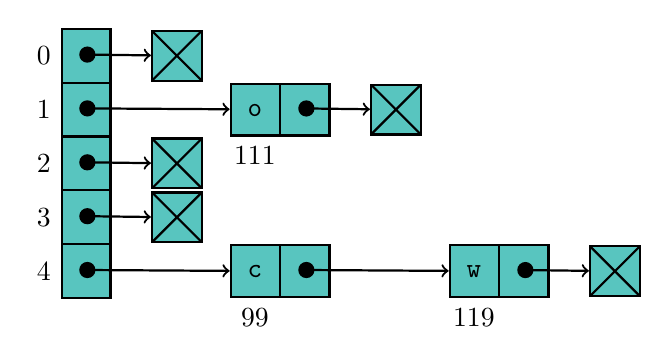
\begin{tikzpicture}[
      thick,
  myrect/.style={
    draw,
    fill=myseagreen,
    rectangle split,
    rectangle split parts=#1,
    rectangle split part align=left,
    text width=2.5ex,
    text centered
    },
	hrect/.style={
    draw,
    fill=myseagreen,
    rectangle split,
    rectangle split horizontal,
    rectangle split parts=#1,
    rectangle split part align=left,
    text width=2.5ex,
    text centered
    }
      ]

\node[myrect=5]
	(array)
  {
  					\strut 
  \nodepart{two}	\strut 
  \nodepart{three}	\strut 
  \nodepart{four}	\strut
  \nodepart{five}	\strut 
  };
\foreach \Valor [count=\Valori from 0] in {one ,two ,three ,four ,five }
  \node[left] at (array.\Valor west) {\Valori};

\node[squarecross] [right=5mm] at (array.one east) (n1) {\strut};
\draw[*->] ($(array.one)+(0.1,0.1)$) -- (n1);

\node[hrect=2] [right=15mm] at (array.two east) (n2) {\strut \texttt{o} \nodepart{two} \strut };
\node[below] at (n2.one south) {111};
\draw[*->] ($(array.two)+(0.1,0.1)$) -- (n2);

\node[squarecross] [right=5mm] at (n2.two east) (m2) {\strut};
\draw[*->] ($(n2.two)+(0.1,0.1)$) -- (m2);

\node[squarecross] [right=5mm] at (array.three east) (n3) {\strut};
\draw[*->] ($(array.three)+(0.1,0.1)$) -- (n3);

\node[squarecross] [right=5mm] at (array.four east) (n4) {\strut};
\draw[*->] ($(array.four)+(0.1,0.1)$) -- (n4);

\node[hrect=2] [right=15mm] at (array.five east) (n5) {\strut \texttt{c} \nodepart{two} \strut };
\node[below] at (n5.one south) {99};
\draw[*->] ($(array.five)+(0.1,0.1)$) -- (n5);

\node[hrect=2] [right=15mm] at (n5.two east) (o5) {\strut \texttt{w} \nodepart{two} \strut };
\node[below] at (o5.one south) {119};
\draw[*->] ($(n5.two)+(0.1,0.1)$) -- (o5);

\node[squarecross] [right=5mm] at (o5.two east) (m5) {\strut};
\draw[*->] ($(o5.two)+(0.1,0.1)$) -- (m5);

% c 99 o 111 w 119

\end{tikzpicture}
\end{center}

If we use a good hash function and a reasonable array size, collisions will almost always be pretty evenly spread across the array. Then, since we store everything using an array, the hash table provides probabilistic $O(1)$ time complexities for insertion, deletion, and search.

The Java set implementation of a hash table is the \texttt{HashSet}. The C++11\footnote{added recently; not included in C++} set implementation of a hash table is the \texttt{unordered\_set}.

\begin{center}
    \begin{tabular}{ | p{5cm} | p{5cm} | p{5cm} | }
      \hline
      \textbf{Function}	&	\textbf{Java, \texttt{HashSet}}	&	\textbf{C++11, \texttt{unordered\_set}} \\ \hline
      \textit{insert}		&	\texttt{boolean add(E e)}	&	\texttt{void insert (const value\_type\& val)} \\ \hline
      \textit{search}		&	\texttt{boolean contains(Object o)}	&	\texttt{size\_type count (const value\_type\& val) const}\footnote{1 if in the \texttt{set}, 0 otherwise.}	\\ \hline
      \textit{delete}		&	\texttt{boolean	remove(Object o)}		&	\texttt{size\_type erase (const value\_type\& val)}, \texttt{void erase (iterator position)} \\ \hline
      \textit{size} & \texttt{int size()} & \texttt{size\_type size() const} \\ \hline
    \end{tabular}
  \end{center}

\section{Map}

A map is very similar to a set. A map is simply a function that takes a key to a value. Generics for maps therefore have two arguments: one for the key and one for the value. Consider the following Java \texttt{Map} from \texttt{String}s to \texttt{String}s.

\begin{mylstlisting}
Map<String, String> email = new TreeMap<String, String>();
email.put("Samuel Hsiang", "samuel.c.hsiang@gmail.com");
\end{mylstlisting}

As a map is a function, its domain, or the keys of the map, form a set, though the values need not be unique.

\texttt{Map} is a Java interface. The \texttt{TreeMap} is the \texttt{Map} variant of the \texttt{TreeSet}; similarly, the \texttt{HashMap} is the \texttt{Map} variant of the \texttt{HashSet}. \texttt{map} is the C++ implementation of a balanced binary search tree map, while \texttt{unordered\_map} is the C++11 implementation of a hash table.

\begin{center}
    \begin{tabular}{ | p{5cm} | p{5cm} | p{5cm} | }
      \hline
      \textbf{Function}	&	\textbf{Java, \texttt{TreeMap}}	&	\textbf{C++, \texttt{map}} \\ \hline
      \textit{insert} and \textit{update}	value	&	\texttt{V put(K key, V value)}	&	\texttt{mapped\_type\& operator[] (const key\_type\& k)}\footnote{Works like an array or \texttt{vector}.} \\ \hline
      \textit{access} & \texttt{V get(Object key)} & \texttt{mapped\_type\& operator[] (const key\_type\& k)} \\ \hline
      \textit{delete} & \texttt{V remove(Object key)} &	\texttt{size\_type erase (const key\_type\& val)}, \texttt{void erase (iterator position)} \\ \hline
      \textit{size} & \texttt{int size()} & \texttt{size\_type size() const} \\ \hline
      set of keys	&  \texttt{Set<K> keySet()} & no implementation \\ \hline
      other useful \textit{search} functions	& \multicolumn{2}{c |}{just look in the API >.<} \\ \hline
    \end{tabular}
\end{center}

\begin{center}
    \begin{tabular}{ | p{5cm} | p{5cm} | p{5cm} | }
      \hline
      \textbf{Function}	&	\textbf{Java, \texttt{HashMap}}	&	\textbf{C++11, \texttt{unordered\_map}} \\ \hline
      \textit{insert} and \textit{update}	value	&	\texttt{V put(K key, V value)}	&	\texttt{mapped\_type\& operator[] (const key\_type\& k)} \\ \hline
      \textit{access} & \texttt{V get(Object key)} & \texttt{mapped\_type\& operator[] (const key\_type\& k)} \\ \hline
      \textit{delete} & \texttt{V remove(Object key)} &	\texttt{size\_type erase (const key\_type\& val)}, \texttt{void erase (iterator position)} \\ \hline
      \textit{size} & \texttt{int size()} & \texttt{size\_type size() const} \\ \hline
      set of keys	&  \texttt{Set<K> keySet()} & no implementation \\ \hline
    \end{tabular}
\end{center}

\section{Big Integer}

A big int is for times when you need integers greater than $2^{63}-1$, when int and long just aren't large enough. The way it works is it stores a number as an array of ints. Each value in the array represents a digit in some very large base. Addition and subtraction can be done in the standard way. Generally multiplying two big ints is not necessary on contests, but it can be sped up using multiplication algorithms like Karatsuba.

\texttt{BigInteger} is in \texttt{java.math}, but C++ does not have an implementation.


\chapter{Big Ideas}

In this chapter we'll discuss some general ideas for solving problems. Starting in this chapter I'm going to shift from language-specific terms, like PriorityQueue and TreeMap, to more general terms, like binary heap and binary search tree. Algorithms I present will no longer be in the form of concrete Java code but rather in a more abstract pseudocode.

\section{Complete Search}

Sometimes the best way is simply to try everything. This could be the intended solution (check the complexity of a complete search and compare it against the time limits), or we may be just coding a brute force to squeeze out a few extra points from an intractable problem at the end of a contest. Either way, the order in which we search can make or break the code.

Suppose we wanted to solve the game of chess. The placement of the pieces on the board and a toggle for whether black or white is to move represents a game state. The set of legal moves maps this game state to one set of states and another set of states to this game state.

We can therefore think of the different states as vertices in a very large directed graph. Methods we use for solving chess, or any other problem, are identical to ways of traversing graphs, especially trees.

\subsection{Depth-First Search}

\textit{Depth-first search} is the most simple of the searches. A depth-first search called on a vertex $v$ in the search tree recursively calls itself on each of the children of $v$. To go back to the chess example, a DFS would begin with one possible first move, like a3, and test \textit{every possible move sequence} beginning with a3 before moving on to a second possible first move, like a4.

A quick note on recursive processes: The \textit{run-time stack} keeps track of our position and data that go out of scope when we jump into a new function. This stack allows us to call functions within functions safely. Recursion is dangerous in contest programming because the run-time stack is slow and can easily balloon in size, crashing the program. For this reason do not hesitate to use your own stack in an iterative process in practice, though I often describe processes as recursive as they are easier to understand, code, and debug in this form.

Now it is painfully obvious that strictly using a DFS is not preferable in computer chess. The computer would certainly never finish testing every move sequence beginning with a3 and therefore would not consider more standard, and likely better, moves like e4.

\subsection{Breadth-First Search}

\textit{Breadth-first search} traverses the search tree level by level. We keep track of a queue that stores each level's state. At each step we pop off the first element in the queue and add the states that it can reach to the end of the queue. In this way, we explore those states only after we explore all the states associated with a lower level. In the chess example, we would store all 20 possible first moves in the queue, and for each first move, we add all possible second moves to the end of the queue.

This means that we search all possible states of a certain depth at roughly the same time, but we need to store the data associated with each of these states, and this can be quite costly in terms of memory.

BFS is the better choice over DFS when we are asked for the ``smallest'' answer, which is often associated with the lowest level.

\subsection{Depth-First Search with Iterative Deepening}

\textit{Depth-first search with iterative deepening} is a DFS that only searches up to a certain level in the search tree before stopping and heading back to lower levels. If it turns out the search did not find anything in the first $N$ levels, we broaden the search to the first $N+1$ levels with another DFS, hence iterative deepening. This method of searching is slower than a BFS, but maintains the nice BFS property of finding the ``smallest'' answer first while shedding the memory harness that holds the BFS back.

DFSID is the closest to what we do when analyzing an actual chess game. We make a move in our minds and test its performance against whatever the opponent might make as his move, tracing the game around 3-4 moves deep before testing another possible move.

\section{Greedy Algorithm}

The main problem with any of the searches described above is they are exponential in nature. A \textit{greedy algorithm} is one that takes the ``best'' possible option at each step, essentially disregarding any other possible option. To find the best solution for $n=4$, we consider only the best solution for $n=3$ and no other possible solution. The approach of maximizing at each step clearly does not always work, as the locally optimal choice is not necessarily globally optimal. Always moving in the direction of a target, for example, fails if there is a wall in the way. However, if the greedy algorithm can solve a problem, the code runs very quickly.

One problem that cannot be solve using the greedy approach is the integer knapsack problem. It's important to be able to catch an incorrect greedy algorithm, and one classic
example involves finding the most efficient way to make change. Given a sequence of coin denominations ($d_i$, where $1 \le i \le n$), with $d_1 = 1$, find the smallest number of coins necessary that sum to some value $V$. The greedy approach takes the most valuable coin that doesn't overshoot $V$ and adds it to our set until we achieve $V$. One counterexample is $v_1=1$, $v_2=3$, $v_3=4$ and $V = 6$. The greedy algorithm chooses $4+1+1$, which is worse than $3+3$. Note however that greedy algorithm still always works for some sets of coin values, like United States currency. Don't let the fact that the greedy algorithm works for the most obvious example fool you.

The greedy algorithm combined with ideas from dynamic programming constitute \textit{best-first search}, a category of searches that includes the Dijkstra algorithm for shortest paths.

\section{Binary Searching on the Answer}

Suppose that the problem we need to solve is finding the minimum number $M$ such that some property holds. That is, the property holds for any $x \ge M$ but does not hold for $x < M$. Perhaps the best approach we have so far for finding this $M$ is simply trying all the numbers from 1 to $M$. However, this linear search is clearly inefficient.

The nature of this problem should remind you of some other search technique. Oftentimes, with problems of this property, it is easy to check whether some condition holds for some given $x$. In this case, it is much easier to binary search on $M$ rather than find it some other way.

\section{Dynamic Programming}

The idea behind dynamic programming is to avoid doing the same thing twice. Two nodes in the search tree described in the complete search techniques might very well represent the same state. For example, two different sets of initial moves could result in the same chessboard configuration, and if we already calculated who has the winning or losing position in that configuration, we ought to remember that fact somehow so we don't need to calculate it again. Of course, however, actually keeping track of every possible game state is intractable by both time and memory constraints.

\subsection{Standard Dynamic Programming}

Here's a much more reasonable problem. Given a sequence of $N \le 10,000$ integers, what is the maximum decreasing subsequence? A subsequence does not have to consist of consecutive terms in the original sequence.

\begin{center}
{
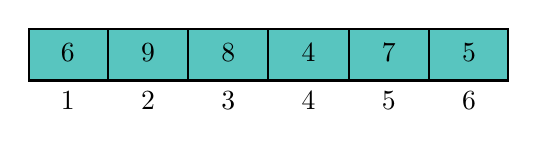
\begin{tikzpicture}[
  thick,
  myrect/.style={
    draw,
    fill=myseagreen,
    rectangle split,
    rectangle split horizontal,
    rectangle split parts=#1,
    rectangle split part align=left,
    text width=5ex,
    text centered
    },
  mycallout/.style={
    shape=rectangle callout,
    rounded corners,
    fill=mysalmon,
    callout absolute pointer={#1},
    callout pointer width=1cm
  }  
]

\node[myrect=6]
  (array)
  {
  					\strut 6
  \nodepart{two}	\strut 9
  \nodepart{three}	\strut 8
  \nodepart{four}	\strut 4
  \nodepart{five}	\strut 7
  \nodepart{six}	\strut 5
  };
\foreach \Valor [count=\Valori from 1] in {one ,two ,three , four , five , six }
  \node[below] at (array.\Valor south) {\Valori};

\end{tikzpicture}
}
\end{center}

The natural complete search approach would be to use recursion, or DFS. When we process an element in the list, we recursively process all elements that come after it and choose the one that gives the maximum subsequence.

\noindent \begin{minipage}{\textwidth}
\begin{algorithmic}
\Function{Process}{$i$}
\State $max \gets 0$
\For{$j\equiv i+1,N$}
	\If{$value(i) > value(j)$}
		\State $x \gets \Call{Process}{$j$}$
		\If{$x > max$}
			\State $max \gets x$
		\EndIf
	\EndIf
\EndFor
\State \Return $max + 1$
\EndFunction
\end{algorithmic}
\end{minipage}

However, this algorithm is exponential. In the worst case, it is $O(2^N)$. We notice a lot of repetition: processing the 9 in the list above, for example, requires finding the longest subsequences beginning with 8, 4, 7, and 5, while processing 8 requires finding subsequences for 4, 7, and 5. It seems silly to do the same task twice, so we'll keep track of the length of the longest subsequence in a separate array.

\noindent \begin{minipage}{\textwidth}
\begin{algorithmic}
\Function{Process}{$i$}
\If{$i$ has already been processed}
	\State \Return $dp(i)$
\EndIf
\State $max \gets 0$
\For{$j\equiv i+1,N$}
	\If{$value(i) > value(j)$}
		\State $x \gets \Call{Process}{j}$
		\If{$x > max$}
			\State $max \gets x$
		\EndIf
	\EndIf
\EndFor
\State $dp(i) \gets max + 1$
\State \Return $max + 1$
\EndFunction
\end{algorithmic}
\end{minipage}

This reduces the complexity of the algorithm to $O(n^2)$. Note that to process an index, we must process first all later indices. This imposes a natural ordering in which to process the indices: in reverse. This idea lends itself to a nice iterative solution.

\noindent \begin{minipage}{\textwidth}
\begin{algorithmic}
\For{$i \equiv N,1$}
	\Comment $i$ goes in reverse
	\State $max \gets 0$
	\For{$j\equiv i+1,N$}
		\If{$value(i) > value(j)$}
			\If{$dp(j) > max$}
				\State $max \gets dp(j)$
			\EndIf
		\EndIf
	\EndFor
	\State $dp(i) \gets max + 1$
\EndFor
\end{algorithmic}
\end{minipage}

The answer to the original problem is then the maximum value of $dp(i)$ for all $i$. For this specific problem, it's relatively easy to speed up the algorithm to $O(\log{n})$ by replacing the linear search with something else.

The integer knapsack problem is another example where dynamic programming may be useful. \textit{Knapsack problems} are a family of problems with the following form:

We are given a list of $K$ objects each assigned an availability, a size, and a value. We have a total amount of ``space'' available in our knapsack and need to find the set of objects from our list that maximizes the total the value of objects in the set such that the total size does not exceed the space and the number of times we take one particular object does not exceed its availability.

Dynamic programming yields a straightforward $O(NK)$ solution. See if you can find it. Note, however, if $N$ is very large, this solution is no longer practical. In general, the knapsack problem is NP-complete, so don't think dynamic programming works on everything!

\subsection{Dynamic Programming over Subsets ($n2^n$ DP)}

Consider the following problem:

(USACO December 2014, guard)
Farmer John and his herd are playing frisbee.  Bessie throws the
frisbee down the field, but it's going straight to Mark the field hand
on the other team!  Mark has height $H$ ($1 \le H \le 1,000,000,000$), but
there are $N$ cows on Bessie's team gathered around Mark ($2 \le N \le 20$).
They can only catch the frisbee if they can stack up to be at least as
high as Mark.  Each of the $N$ cows has a height, weight, and strength.
A cow's strength indicates the maximum amount of total weight of the
cows that can be stacked above her.  

Given these constraints, Bessie wants to know if it is possible for
her team to build a tall enough stack to catch the frisbee, and if so,
what is the maximum safety factor of such a stack.  The safety factor
of a stack is the amount of weight that can be added to the top of the
stack without exceeding any cow's strength.

We can try the $O(N!)$ brute force, trying every permutation of cows possible. However, this is far too slow. $N \le 20$ hints at an exponential solution, so we think of trying every possible subset of the cows. Given a subset $S$ of cows, the height reached is the same, so perhaps we sort the subset by strength, and put the strongest cow on the bottom. We see that this greedy approach fails: suppose that the first cow has weight 1 and strength 3 and the second cow has weight 4 and strength 2. Greedy would tell us to put the first cow on the bottom, but this fails, while putting the second cow on the bottom succeeds.

When greedy fails, the next strategy we look at is dynamic programming. To decide whether $S$ is stable, we have to find whether there exists a cow $j$ in $S$ that can support the weight of all the other cows in $S$. But how do we know whether the set $S \setminus \{j\}$ is stable? This is where dynamic programming comes in.

This leads to a $O(N 2^N)$ solution. This seems like a pain to code iteratively, but there is a nice fact about subsets: there is a cute bijection from the subsets of $\{0,1,2, \ldots, N-1\}$ to the integers from 0 to $2^N - 1$. That is, the subset $\{0,2,5,7\}$ maps to $2^0 + 2^2 + 2^5 + 2^7 = 165$ in the bijection. We call this technique \textit{masking}. We require all the subsets of $S$ to be processed before $S$ is processed, but that property is also handled by our bijection, since subtracting a power of 2 from a number decreases it. With a little knowledge of bit operators, this can be handled easily.

\noindent \begin{minipage}{\textwidth}
\begin{algorithmic}
\For{$i\gets 0, 2^N-1$}
	\Comment $i$ represents the subset $S$
	\State $dp(i) \gets -1$
	\ForAll{$j \in S$}
		\Comment $j \in S$ satisfy \texttt{i \& (1 << j) != 0}
		\State $alt \gets \min(dp(i-2^j), strength(j) - \sum_{k \in S \setminus \{j\}} weight(k))$
		\If{$dp(i) < alt$}
			\State $dp(i) \gets alt$
		\EndIf
	\EndFor
\EndFor
\end{algorithmic}
\end{minipage}

\texttt{\&} is the bitwise and function, while \texttt{<<} is the left shift operator.

Brian Dean compiled some standard dynamic programming problems with animations and analyses. Practice dynamic programming here: \url{http://people.cs.clemson.edu/~bcdean/dp_practice/}


\chapter{Graph Algorithms}

In this chapter we explore some famous graph theory results.

\section{Connected Components}

A \textit{connected component} of an undirected graph is a subgraph such that, for any two vertices in the component, there exists a path from one to the other. The diagram illustrates three connected components of a graph, where each vertex is colored togethwer with its associated component.

\begin{center}
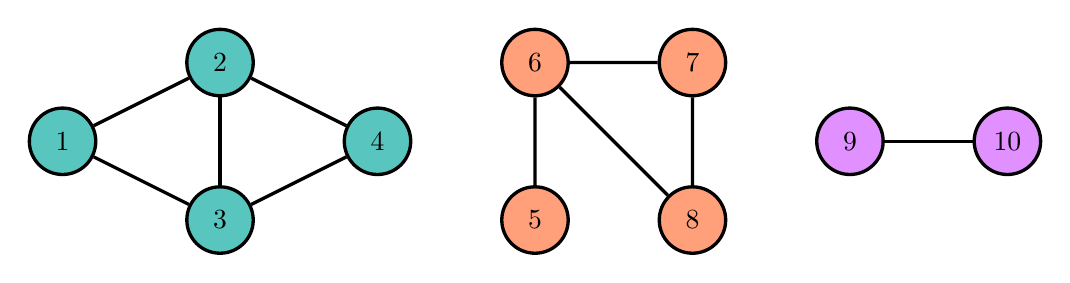
\begin{tikzpicture}[very thick,level/.style={sibling distance=70mm/#1}]
\draw (0, 0) node [vertex] (n1) {1};
\draw (2, 1) node [vertex] (n2) {2};
\draw (2, -1) node  [vertex] (n3) {3};
\draw (4, 0) node [vertex] (n4) {4};
\draw (n1) -- (n2);
\draw (n2) -- (n3);
\draw (n3) -- (n4);
\draw (n2) -- (n4);
\draw (n1) -- (n3);
\draw (6, -1) node [vertex, fill=mysalmon] (n5) {5};
\draw (6, 1) node [vertex, fill=mysalmon] (n6) {6};
\draw (8, 1) node [vertex, fill=mysalmon] (n7) {7};
\draw (8, -1) node [vertex, fill=mysalmon] (n8) {8};
\draw (n5) -- (n6) -- (n7) -- (n8) -- (n6);
\draw (10, 0) node[vertex, fill=mypurple] (n9) {9};
\draw (12, 0) node[vertex, fill=mypurple] (n10) {10};
\draw (n9) -- (n10);
\end{tikzpicture}
\end{center}

A \textit{strongly connected component} of a directed graph is a subgraph such that every vertex in the component can be reached from any other vertex in the component.

\begin{center}
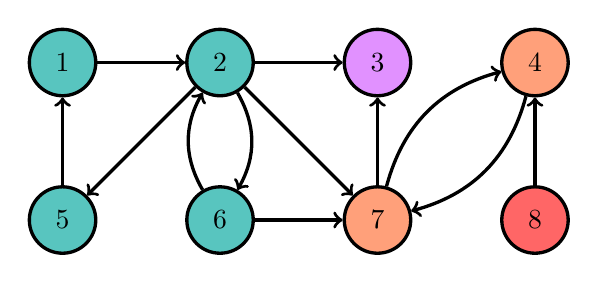
\begin{tikzpicture}[very thick,level/.style={sibling distance=70mm/#1}]
\draw (0, 0) node [vertex] (n1) {5};
\draw (2, 0) node [vertex] (n2) {6};
\draw (4, 0) node [vertex, fill=mysalmon] (n3) {7};
\draw (6, 0) node [vertex, fill=myred] (n4) {8};
\draw (0, 2) node [vertex] (m1) {1};
\draw (2, 2) node [vertex] (m2) {2};
\draw (4, 2) node [vertex, fill=mypurple] (m3) {3};
\draw (6, 2) node [vertex, fill=mysalmon] (m4) {4};
\draw[->] (m1) -- (m2);
\draw[->] (m2) -- (n1);
\draw[->] (n1) -- (m1);
\draw[->] (n2) edge [bend left] (m2);
\draw[->] (m2) edge [bend left] (n2);
\draw[->] (n2) -- (n3);
\draw[->] (m2) -- (m3);
\draw[->] (m2) -- (n3);
\draw[->] (n3) -- (m3);
\draw[->] (n3) edge [bend left] (m4);
\draw[->] (m4) edge [bend left] (n3);
\draw[->] (n4) -- (m4);
\end{tikzpicture}
\end{center}

Finding the connected components of an undirected graph is a straightforward problem, while finding the strongly connected components of a directed graph is more complicated.

\subsection{Flood Fill}

Really any kind of search method solves the undirected graph connected components problem. We could use recursion with a depth-first search. To avoid using the run-time stack, we could use a queue to perform a breadth-first search. Both of these run in $O(E+V)$ time. I would recommend in general to use the BFS.

\subsection{Union-Find (Disjoint Set Union)}

The union-find data structure is another way for us to solve the connected components problem. Union-find is unique from the other search techniques in that it can process input as it is presented, edge by edge. This also means it is possible to add more edges at the end, therefore changing the graph, while still running quickly. An algorithm that works like this is an \textit{online algorithm}, while an algorithm that requires all the input data presented at the beginning is an \textit{offline algorithm}.

A natural idea for solving the connected components problem is for each vertex to maintain a pointer to another vertex it's connected to, forming a \textit{forest}, or collection of trees. To check whether two elements are in the same component, simply trace the tree up to the root by jumping up each pointer.

\begin{center}
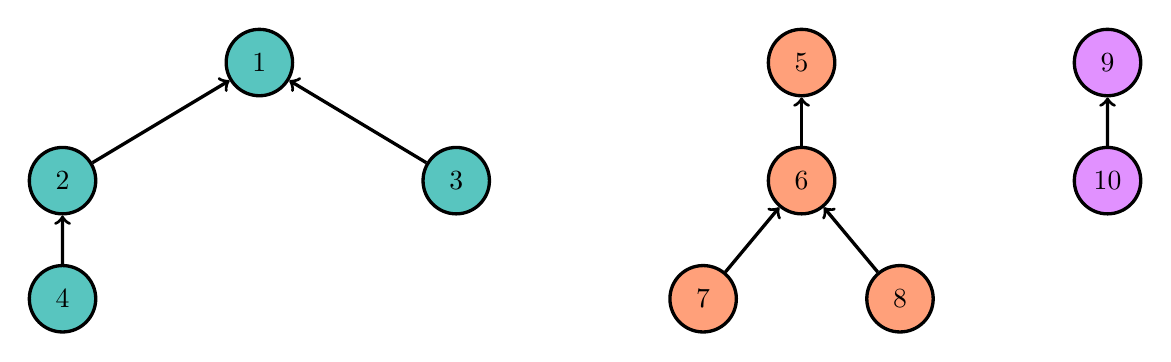
\begin{tikzpicture}[very thick,edge from parent/.style={draw,<-},level/.style={sibling distance=50mm/#1}]
\node [vertex, fill = mysalmon] (r2) {5}
  child {
      node [vertex, fill = mysalmon] {6}
      child { node [vertex, fill=mysalmon] {7} }
      child { node [vertex, fill=mysalmon] {8} }
  };

\node [vertex] [left=6cm of r2] (r1) {1}
  child {
    node [vertex] {2}
    child {
      node [vertex] {4}
    }
  }
  child {node [vertex] {3} };
  
\node [vertex, fill=mypurple] [right=3cm of r2] (r3) {9}
  child { node [vertex, fill=mypurple] {10} };
\end{tikzpicture}
\end{center}

The idea of a pointer can easily be stored within an array.

\begin{center}
{
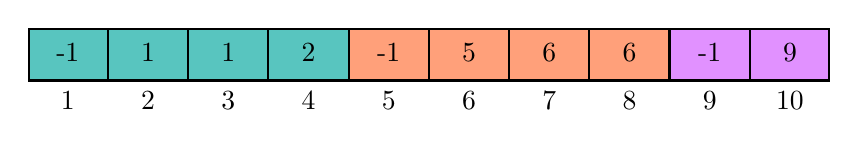
\begin{tikzpicture}[
  thick,
  myrect/.style={
    draw,
    rectangle split,
    rectangle split horizontal,
    rectangle split parts=#1,
    rectangle split part align=left,
    text width=5ex,
    text centered
    },
  mycallout/.style={
    shape=rectangle callout,
    rounded corners,
    fill=mysalmon,
    callout absolute pointer={#1},
    callout pointer width=1cm
  }  
]

\node[myrect=10, rectangle split part fill={myseagreen, myseagreen, myseagreen, myseagreen, mysalmon, mysalmon, mysalmon, mysalmon, mypurple, mypurple}]
  (array1)
  {
  					\strut -1
  \nodepart{two}	\strut 1
  \nodepart{three}	\strut 1
  \nodepart{four}	\strut 2
  \nodepart{five}	\strut -1
  \nodepart{six}	\strut 5
  \nodepart{seven}	\strut 6
  \nodepart{eight}	\strut 6
  \nodepart{nine}	\strut -1
  \nodepart{ten}	\strut 9
  };
\foreach \Valor [count=\Valori from 1] in {one ,two ,three ,four ,five ,six ,seven ,eight ,nine ,ten }
  \node[below] at (array1.\Valor south) {\Valori};

\end{tikzpicture}
}
\end{center}

We want to support two operations: $find(v)$, which returns the root of the tree containing $v$, and $union(u,v)$, which merges the components containing $u$ and $v$. This second operation is easy given the first; simply set the pointer of $find(u)$ to be $find(v)$.

$union(4, 6)$, unoptimized:

\begin{center}
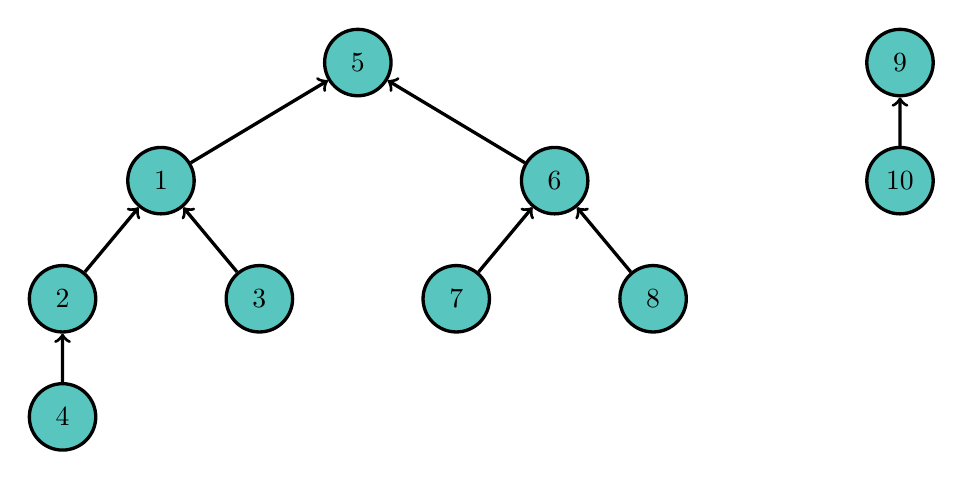
\begin{tikzpicture}[very thick,edge from parent/.style={draw,<-},level/.style={sibling distance=50mm/#1}]
\node [vertex] (r2) {5}
	child {
    node [vertex] (r1) {1}
	  child {
 	   node [vertex] {2}
  	  child {
   	   node [vertex] {4}
  	  }
	  }
 	 child {node [vertex] {3} }
  }
  child {
  node [vertex] {6}
		child { node [vertex] {7} }
   		child { node [vertex] {8} }
    };
\node [vertex] [right=6cm of r2] (r3) {9}
  child { node [vertex] {10} };
\end{tikzpicture}
\end{center}

A problem quickly arises -- the $find$ operation threatens to become linear. There are two simple things we can do to optimize this.

The first is to always add the shorter tree to the taller tree, as we want to minimize the maximum height. An easy heuristic for the height of the tree is simply the number of elements in that tree. We can keep track of the size of the tree with a second array. This heuristic is obviously not perfect, as a larger tree can be shorter than a smaller tree, but it turns out with our second optimization that this problem doesn't matter.

The second fix is to simply assign the pointer associated with $v$ to be $find(v)$ at the end of the $find$ operation. We can design $find(v)$ to recursively call $find$ on the pointer associated with $v$, so this fix sets pointers associated with nodes along the entire chain from $v$ to $find(v)$ to be $find(v)$. These two optimizations combined make the $union$ and $find$ operations $O(\alpha (V))$, where $\alpha(n)$ is the inverse Ackermann function, and for all practical values of $n$, $\alpha(n) < 5$.

$find(4)$, optimized:

\begin{center}
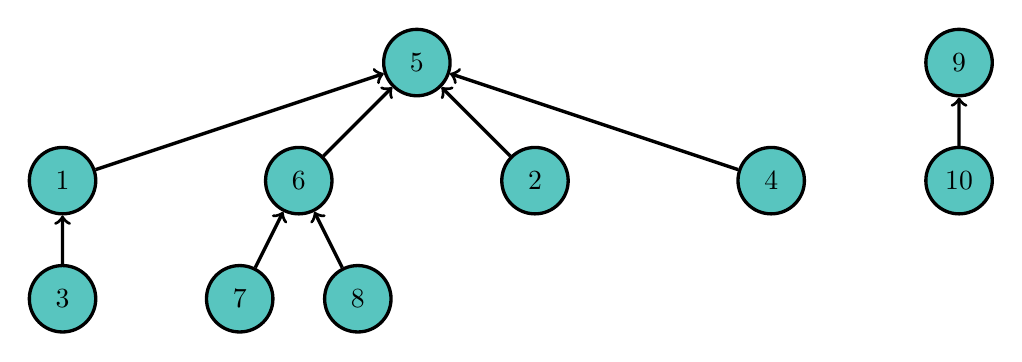
\begin{tikzpicture}[very thick,edge from parent/.style={draw,<-},level/.style={sibling distance=30mm/#1}]
\node [vertex] (r2) {5}
	child {
    node [vertex] (r1) {1}
 	 child {node [vertex] {3} }
  }
  child {
  node [vertex] {6}
		child { node [vertex] {7} }
   		child { node [vertex] {8} }
    }
  child {node[vertex] {2}}
  child {node[vertex] {4}};
\node [vertex] [right=6cm of r2] (r3) {9}
  child { node [vertex] {10} };
\end{tikzpicture}
\end{center}

\begin{algorithm}[H]
\caption{Union-Find}
%\label{}
\begin{algorithmic}
\Function{Find}{$v$}
	\If {$v$ is the root}
		\State \Return $v$
    \EndIf
    \State $parent(v) \gets \Call{Find}{parent(v)}$
    \State \Return $parent(v)$
\EndFunction
\Function{Union}{$u$, $v$}
	\State $uRoot \gets \Call{Find}{u}$
	\State $vRoot \gets \Call{Find}{v}$
    \If {$uRoot = vRoot$}
		\State \Return
	\EndIf
    \If {$size(uRoot)<size(vRoot)$}
    	\State $parent(uRoot) \gets vRoot$
        \State $size(vRoot) \gets size(uRoot) + size(vRoot)$
    \Else
    	\State $parent(vRoot) \gets uRoot$
        \State $size(uRoot) \gets size(uRoot) + size(vRoot)$
    \EndIf
\EndFunction
\end{algorithmic}
\end{algorithm}

\subsection{Tarjan}

Tarjan's algorithm detects strongly connected components in a directed graph. We begin with the DFS traversal of the graph, building a forest (collection of trees). In a DFS, we only traverse each vertex once; this means when we encounter an edge to a vertex we already visited, we move on without calling the DFS on that node. Once we obtain the forest, we can split it into subgraphs that represent our strongly connected components.

Let's work through how we can get the subgraphs representing the strongly connected components from our DFS. Here's the graph from the beginning of this section.

\begin{center}
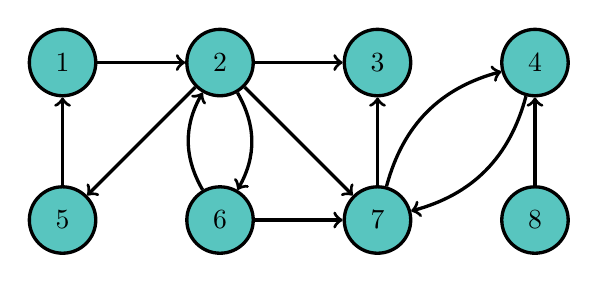
\begin{tikzpicture}[very thick,level/.style={sibling distance=70mm/#1}]
\draw (0, 0) node [vertex] (n1) {5};
\draw (2, 0) node [vertex] (n2) {6};
\draw (4, 0) node [vertex] (n3) {7};
\draw (6, 0) node [vertex] (n4) {8};
\draw (0, 2) node [vertex] (m1) {1};
\draw (2, 2) node [vertex] (m2) {2};
\draw (4, 2) node [vertex] (m3) {3};
\draw (6, 2) node [vertex] (m4) {4};
\draw[->] (m1) -- (m2);
\draw[->] (m2) -- (n1);
\draw[->] (n1) -- (m1);
\draw[->] (n2) edge [bend left] (m2);
\draw[->] (m2) edge [bend left] (n2);
\draw[->] (n2) -- (n3);
\draw[->] (m2) -- (m3);
\draw[->] (m2) -- (n3);
\draw[->] (n3) -- (m3);
\draw[->] (n3) edge [bend left] (m4);
\draw[->] (m4) edge [bend left] (n3);
\draw[->] (n4) -- (m4);
\end{tikzpicture}
\end{center}

It doesn't matter from which node we begin our DFS or the order in which we choose children; in our example, we'll simply choose the node with the minimum label to traverse first. This will result in two trees in our forest, one rooted at 1 and the other rooted at 8.

\begin{center}
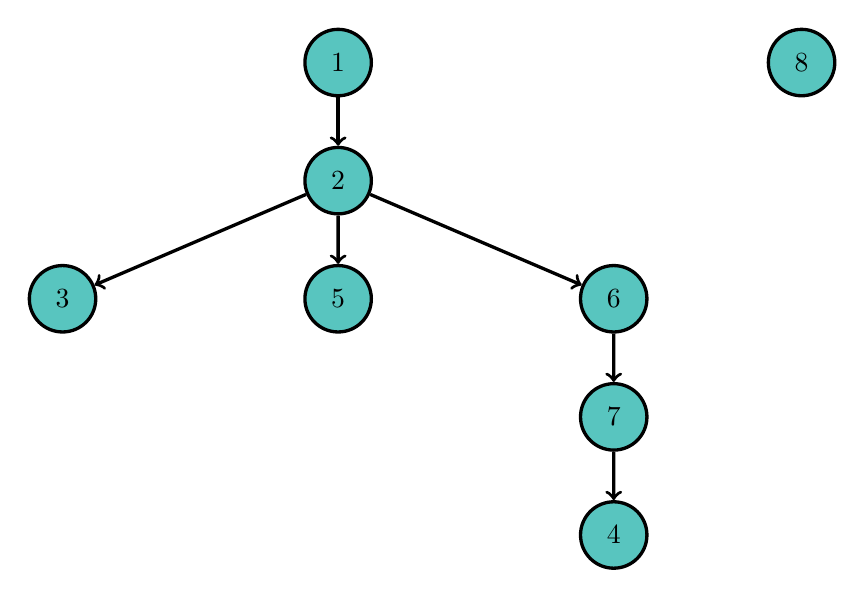
\begin{tikzpicture}[very thick,level/.style={sibling distance=70mm/#1}, edge from parent/.style={draw, ->}]
\node [vertex] (n1) {1}
child {
	node [vertex] (n2) {2}
	child {
		node [vertex] (n3) {3}
	}
	child {
		node [vertex] (n5) {5}
	}
	child {
		node [vertex] (n6) {6}
		child {
			node [vertex] (n7) {7}
			child {
				node [vertex] (n4) {4}
			}
		}
	}
};
\node [vertex] [right=5cm of n1] (n8) {8};
\end{tikzpicture}
\end{center}

Now this by itself is not very useful, as in order to find strongly connected components, we'll need the edges in the directed graph that aren't included in our tree. Here we add the other edges as dashed pointers.

\begin{center}
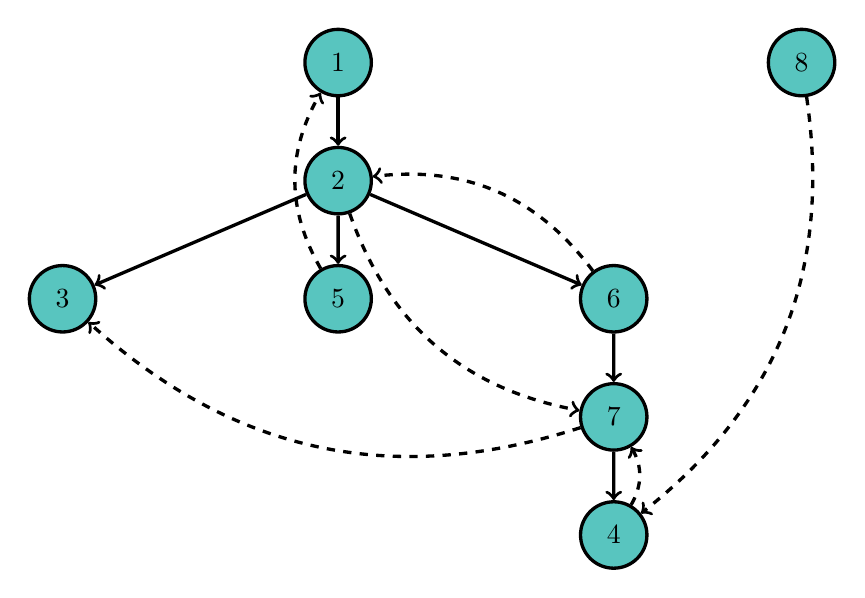
\begin{tikzpicture}[very thick,level/.style={sibling distance=70mm/#1}, edge from parent/.style={draw, ->}]
\node [vertex] (n1) {1}
child {
	node [vertex] (n2) {2}
	child {
		node [vertex] (n3) {3}
	}
	child {
		node [vertex] (n5) {5}
	}
	child {
		node [vertex] (n6) {6}
		child {
			node [vertex] (n7) {7}
			child {
				node [vertex] (n4) {4}
			}
		}
	}
};
\node [vertex] [right=5cm of n1] (n8) {8};
\draw[->, dashed] (n5) edge [bend left] (n1);
\draw[->, dashed] (n6) edge [bend right] (n2);
\draw[->, dashed] (n2) edge [bend right] (n7);
\draw[->, dashed] (n4) edge [bend right] (n7);
\draw[->, dashed] (n8) edge [bend left] (n4);
\draw[->, dashed] (n7) edge [bend left] (n3);
\end{tikzpicture}
\end{center}

Note that strongly connected components are represented by subtrees in the graph. We call the root of the subtree called the root of the strongly connected component.

One edge here is immediately useless. We already know that 2 can reach 7; 7 is in 2's subtree. The fact that there is an edge from 2 to 7 doesn't change anything. Then we have a crucial observation -- the only possible useful extra edges are those that go up to a previous node in the subtree, like the edge from 5 to 1, or those that go ``left'' to a previously-visited vertex, either to a previous branch in the tree, like from 7 to 3, or to a previous subtree entirely, like from 8 to 4.

If a node $v$ has an edge to a direct ancestor in the tree, that means we immediately have a cycle, and therefore the node, its ancestor, and every vertex along the way must be in the same strongly connected component.

Naturally, the ``left'' case is trickier. Suppose $v$ has a left edge to a vertex $u$. We somehow need a way to find out if $u$ has a path back to $v$. We know that $u$ cannot go down the tree to $v$ as $v$ is not in the subtree of $u$ by the way DFS constructed the tree. Therefore, we want to know whether $u$ has a path back up to some common ancestor with $v$. However, again by the way DFS traverses the graph, the entire subtree of $u$ has already been searched before the DFS reaches $v$. We want to exploit this fact with some kind of memoization.

If vertex $v$ was the $n$th vertex visited in the DFS, we'll mark $v$ with the label $order(v) = n$. We'll also keep track of the ``least'' vertex $link(v)=u$ that we know up to that point that $v$ can visit, or the vertex $u$ with the minimum $order(u)$ that $v$ can reach so far.

As we're using a DFS, we'll use a stack $S$ to keep track of nodes we've visited. In a normal DFS on a tree, once we finish exploring a vertex $v$, we pop off $v$ from the stack. This will not be the case for us. A node remains on the stack iff it has a path to some node earlier in the stack.

This means as we explore the descendents of a vertex $v$, we'll know if $v$ has a path back to a previous vertex. That is, if $link(v) < order(v)$, it stays on the stack. If $link(v) = order(v)$, we take it off the stack.

Now we describe Tarjan's algorithm. Here, $num$ represents a global variable that indicates how many vertices have been visited so far.

\begin{algorithm}[H]
\caption{Tarjan}
\begin{algorithmic}
\Function{StrongConnect}{vertex $u$}
	\State $num \gets num + 1$		\Comment increment $num$
	\State $order(u) \gets num$		\Comment set $order(u)$ to smallest unused number
	\State $link(u) \gets order(u)$	\Comment least $order(v)$ accessible is $u$ itself
	\State push $u$ on $S$
	\ForAll{neighbors $v$ of $u$}
		\If{$order(v)$ is undefined}	\Comment $v$ has not been visited
			\State \Call{StrongConnect}{$v$}
			\State $link(u) \gets \min(link(u), link(v))$
		\ElsIf{$v$ is on stack $S$}		\Comment $v$ is in current component
			\State $link(u) \gets \min(link(u), order(v))$
		\EndIf
	\EndFor
	\If{$link(u) = order(u)$}			\Comment $u$ is root of component, create SCC
		\State create new strongly connected component
		\Repeat
			\State $v \gets$ top of $S$
			\State add $v$ to strongly connected component
			\State pop top from $S$
		\Until{$u=v$}
	\EndIf
\EndFunction
\Function{Tarjan}{$G(V,E)$}
	\State $num \gets 0$
	\State initialize new empty stack $S$
	\ForAll{vertices $v \in V$}
		\If{$order(v)$ is undefined}	\Comment $v$ has not been visited
			\State \Call{StrongConnect}{$v$}
		\EndIf
	\EndFor
\EndFunction
\end{algorithmic}
\end{algorithm}

This algorithm runs in $O(V+E)$.

\section{Shortest Path}

A classic. Assign nonnegative weights to each of the edges, where the weight of the edge $(u,v)$ represents the distance from $u$ to $v$. This graph can be either directed or undirected.

\subsection{Dijkstra}

Dijkstra's algorithm solves the single-source shortest path problem. From any vertex, we can compute the shortest path to each of the remaining vertices in the graph. The two formulations of Dijkstra's algorithm run in $O(V^2)$ or $O(E\log{V})$ time, whichever one suits us better. Note that it is possible to do better than $O(E\log{V})$ using a Fibonacci heap. The former works nicely on dense graphs, as $E \approx V^2$, while the latter works better on sparse graphs, as $E \approx V$.

For every vertex $v$ in the graph, we keep track of the shortest known distance $dist(v)$ from the source to $v$, a boolean $visited(v)$ to keep track of which nodes we ``visited,'' and a pointer to the previous node in the shortest known path $prev(v)$ so that we can trace the shortest path once the algorithm finishes.

Dijkstra iteratively ``visits'' the next nearest vertex, updating the distances to that vertex's neighbors if necessary. Therefore, at any step, we have the first however-many nearest vertices to the source, which we call ``visited'' and for which the shortest path is known. We also have the shortest path to all the remaining vertices that stays within the ``visited'' vertices besides for the very last edge, if such a path exists. We claim that the known distance to the closest vertex that has not yet been visited is the shortest distance. We can then ``visit'' that vertex. It shouldn't be hard to prove that this algorithm indeed calculates the shortest path.

The $O(V^2)$ implementation immediately follows.

\begin{algorithm}[H]
\caption{Dijkstra}
\begin{algorithmic}
\ForAll{vertices $v$}
	\State $dist(v) \gets \infty$
	\State $visited(v) \gets 0$
    \State $prev(v) \gets -1$
\EndFor
\State $dist(src) \gets 0$
\While{$\exists v$ s.t. $visited(v)=0$}
	\State $v \equiv v$ s.t. $visited(v)=0$ with min $dist(v)$
    \State $visited(v) \gets 1$
	\ForAll{neighbors $u$ of $v$}
    	\If{$visited(u) = 0$}
    		\State $alt \gets dist(v) + weight(v, u)$
			\If{$alt < dist(u)$}
				\State $dist(u) \gets alt$
   	        	\State $prev(u) \gets v$
			\EndIf
        \EndIf
    \EndFor
\EndWhile
\end{algorithmic}
\end{algorithm}

\begin{center}
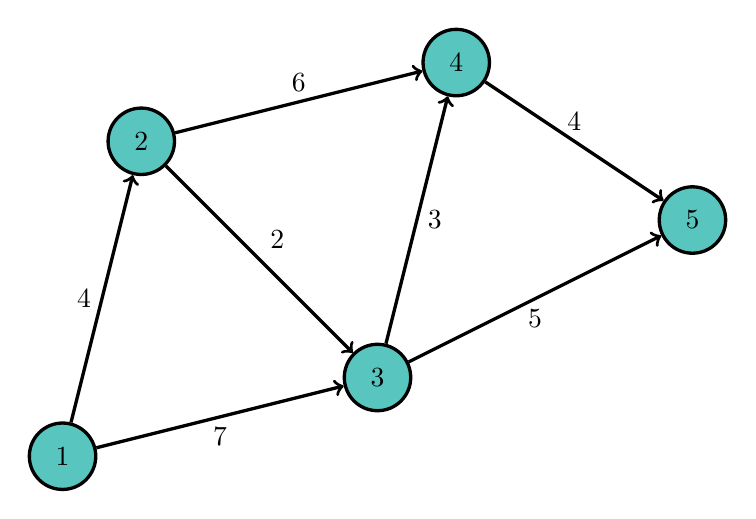
\begin{tikzpicture}[very thick,edge from parent/.style={draw,<-},level/.style={sibling distance=30mm/#1}]
\draw (0, 0) node [vertex] (v1) {1};
\draw (1, 4) node [vertex] (v2) {2};
\draw (4, 1) node [vertex] (v3) {3};
\draw (5, 5) node [vertex] (v4) {4};
\draw (8, 3) node [vertex] (v5) {5};
\draw[->] (v1) -- (v2) node[midway, left] {4};
\draw[->] (v2) -- (v3) node[midway, above right] {2};
\draw[->] (v1) -- (v3) node[midway, below] {7};
\draw[->] (v2) -- (v4) node[midway, above] {6};
\draw[->] (v3) -- (v4) node[midway, right] {3};
\draw[->] (v3) -- (v5) node[midway, below] {5};
\draw[->] (v4) -- (v5) node[midway, above] {4};
\end{tikzpicture}
\end{center}

Let's run Dijkstra's algorithm on the above graph with vertex 1 as the source. We first set all the distances besides the source to be $\infty$.

\begin{center}
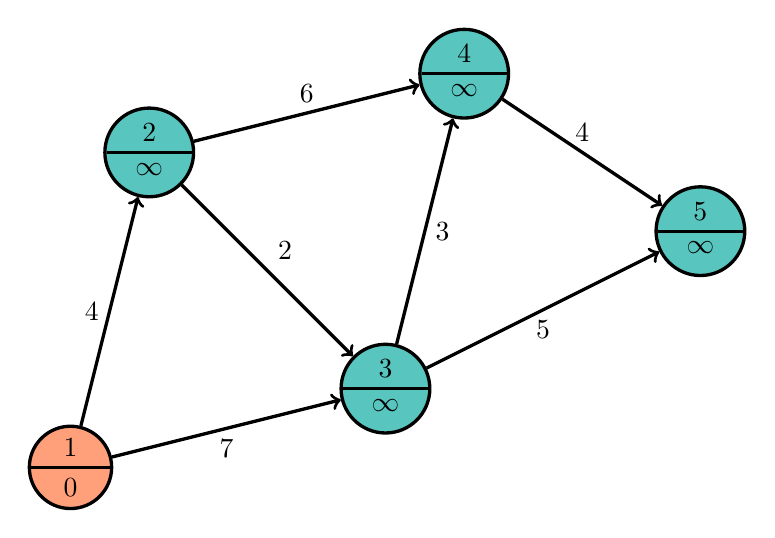
\begin{tikzpicture}[very thick,edge from parent/.style={draw,<-},level/.style={sibling distance=30mm/#1}]
\draw (0, 0) node [splitvertex, fill=mysalmon] (v1) {1\nodepart{lower}0};
\draw (1, 4) node [splitvertex] (v2) {2\nodepart{lower}$\infty$};
\draw (4, 1) node [splitvertex] (v3) {3\nodepart{lower}$\infty$};
\draw (5, 5) node [splitvertex] (v4) {4\nodepart{lower}$\infty$};
\draw (8, 3) node [splitvertex] (v5) {5\nodepart{lower}$\infty$};
\draw[->] (v1) -- (v2) node[midway, left] {4};
\draw[->] (v2) -- (v3) node[midway, above right] {2};
\draw[->] (v1) -- (v3) node[midway, below] {7};
\draw[->] (v2) -- (v4) node[midway, above] {6};
\draw[->] (v3) -- (v4) node[midway, right] {3};
\draw[->] (v3) -- (v5) node[midway, below] {5};
\draw[->] (v4) -- (v5) node[midway, above] {4};
\end{tikzpicture}
\end{center}

Now, we continue choosing the closest unvisited node, mark it as visited, and and update its neighbors.

\begin{center}
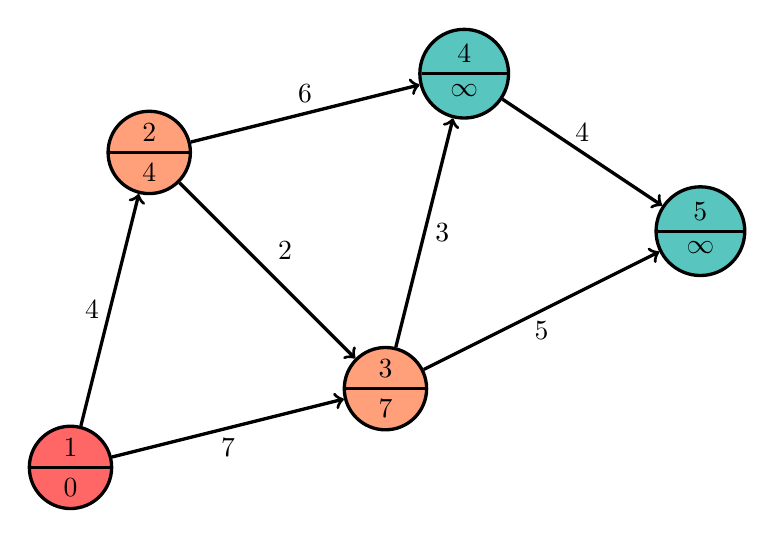
\begin{tikzpicture}[very thick,edge from parent/.style={draw,<-},level/.style={sibling distance=30mm/#1}]
\draw (0, 0) node [splitvertex, fill=myred] (v1) {1\nodepart{lower}0};
\draw (1, 4) node [splitvertex, fill=mysalmon] (v2) {2\nodepart{lower}4};
\draw (4, 1) node [splitvertex, fill=mysalmon] (v3) {3\nodepart{lower}7};
\draw (5, 5) node [splitvertex] (v4) {4\nodepart{lower}$\infty$};
\draw (8, 3) node [splitvertex] (v5) {5\nodepart{lower}$\infty$};
\draw[->] (v1) -- (v2) node[midway, left] {4};
\draw[->] (v2) -- (v3) node[midway, above right] {2};
\draw[->] (v1) -- (v3) node[midway, below] {7};
\draw[->] (v2) -- (v4) node[midway, above] {6};
\draw[->] (v3) -- (v4) node[midway, right] {3};
\draw[->] (v3) -- (v5) node[midway, below] {5};
\draw[->] (v4) -- (v5) node[midway, above] {4};
\end{tikzpicture}
\end{center}

\begin{center}
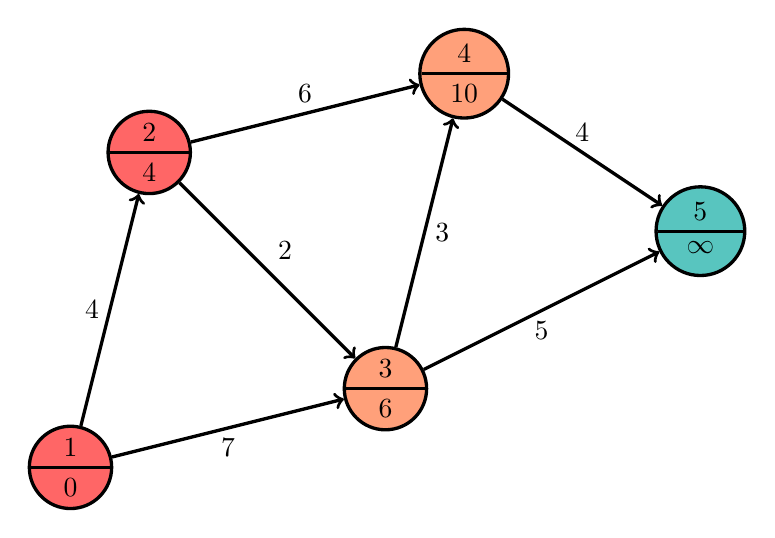
\begin{tikzpicture}[very thick,edge from parent/.style={draw,<-},level/.style={sibling distance=30mm/#1}]
\draw (0, 0) node [splitvertex, fill=myred] (v1) {1\nodepart{lower}0};
\draw (1, 4) node [splitvertex, fill=myred] (v2) {2\nodepart{lower}4};
\draw (4, 1) node [splitvertex, fill=mysalmon] (v3) {3\nodepart{lower}6};
\draw (5, 5) node [splitvertex, fill=mysalmon] (v4) {4\nodepart{lower}10};
\draw (8, 3) node [splitvertex] (v5) {5\nodepart{lower}$\infty$};
\draw[->] (v1) -- (v2) node[midway, left] {4};
\draw[->] (v2) -- (v3) node[midway, above right] {2};
\draw[->] (v1) -- (v3) node[midway, below] {7};
\draw[->] (v2) -- (v4) node[midway, above] {6};
\draw[->] (v3) -- (v4) node[midway, right] {3};
\draw[->] (v3) -- (v5) node[midway, below] {5};
\draw[->] (v4) -- (v5) node[midway, above] {4};
\end{tikzpicture}
\end{center}

\begin{center}
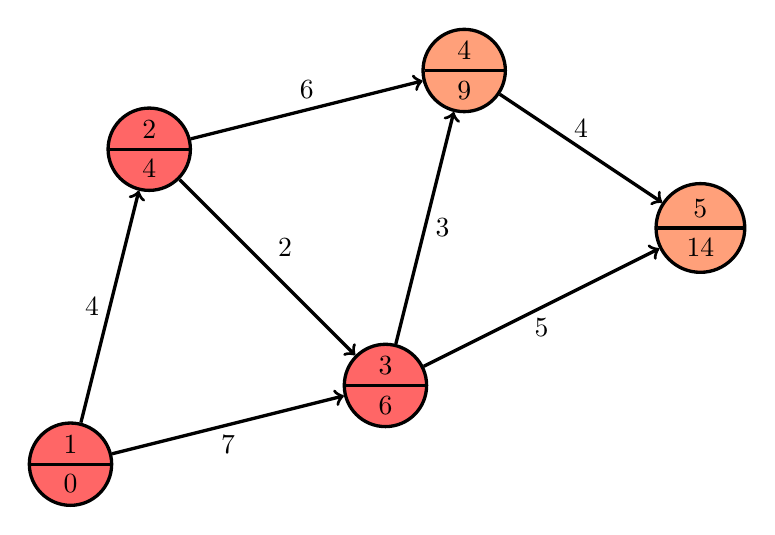
\begin{tikzpicture}[very thick,edge from parent/.style={draw,<-},level/.style={sibling distance=30mm/#1}]
\draw (0, 0) node [splitvertex, fill=myred] (v1) {1\nodepart{lower}0};
\draw (1, 4) node [splitvertex, fill=myred] (v2) {2\nodepart{lower}4};
\draw (4, 1) node [splitvertex, fill=myred] (v3) {3\nodepart{lower}6};
\draw (5, 5) node [splitvertex, fill=mysalmon] (v4) {4\nodepart{lower}9};
\draw (8, 3) node [splitvertex, fill=mysalmon] (v5) {5\nodepart{lower}14};
\draw[->] (v1) -- (v2) node[midway, left] {4};
\draw[->] (v2) -- (v3) node[midway, above right] {2};
\draw[->] (v1) -- (v3) node[midway, below] {7};
\draw[->] (v2) -- (v4) node[midway, above] {6};
\draw[->] (v3) -- (v4) node[midway, right] {3};
\draw[->] (v3) -- (v5) node[midway, below] {5};
\draw[->] (v4) -- (v5) node[midway, above] {4};
\end{tikzpicture}
\end{center}

\begin{center}
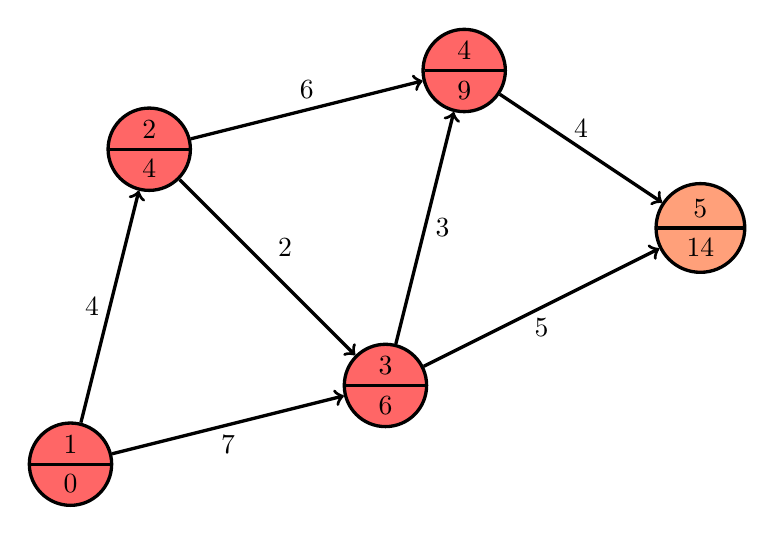
\begin{tikzpicture}[very thick,edge from parent/.style={draw,<-},level/.style={sibling distance=30mm/#1}]
\draw (0, 0) node [splitvertex, fill=myred] (v1) {1\nodepart{lower}0};
\draw (1, 4) node [splitvertex, fill=myred] (v2) {2\nodepart{lower}4};
\draw (4, 1) node [splitvertex, fill=myred] (v3) {3\nodepart{lower}6};
\draw (5, 5) node [splitvertex, fill=myred] (v4) {4\nodepart{lower}9};
\draw (8, 3) node [splitvertex, fill=mysalmon] (v5) {5\nodepart{lower}14};
\draw[->] (v1) -- (v2) node[midway, left] {4};
\draw[->] (v2) -- (v3) node[midway, above right] {2};
\draw[->] (v1) -- (v3) node[midway, below] {7};
\draw[->] (v2) -- (v4) node[midway, above] {6};
\draw[->] (v3) -- (v4) node[midway, right] {3};
\draw[->] (v3) -- (v5) node[midway, below] {5};
\draw[->] (v4) -- (v5) node[midway, above] {4};
\end{tikzpicture}
\end{center}

\begin{center}
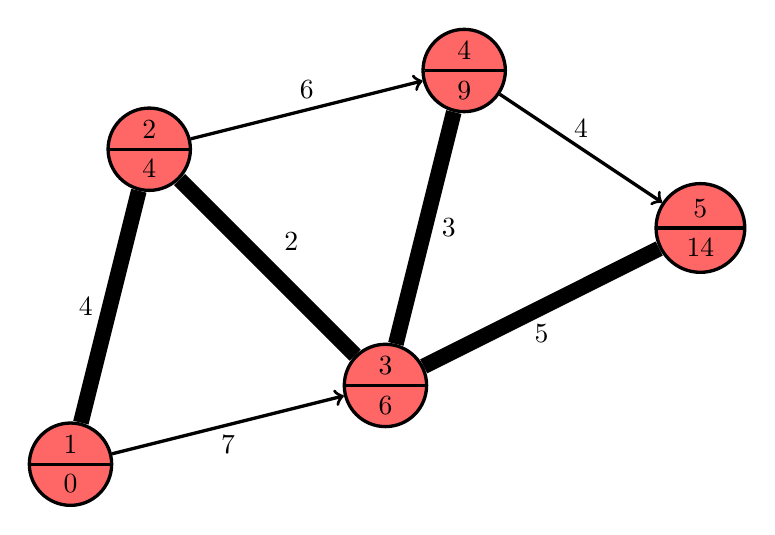
\begin{tikzpicture}[very thick,edge from parent/.style={draw,<-},level/.style={sibling distance=30mm/#1}]
\draw (0, 0) node [splitvertex, fill=myred] (v1) {1\nodepart{lower}0};
\draw (1, 4) node [splitvertex, fill=myred] (v2) {2\nodepart{lower}4};
\draw (4, 1) node [splitvertex, fill=myred] (v3) {3\nodepart{lower}6};
\draw (5, 5) node [splitvertex, fill=myred] (v4) {4\nodepart{lower}9};
\draw (8, 3) node [splitvertex, fill=myred] (v5) {5\nodepart{lower}14};
\draw[line width=2mm] (v1) -- (v2) node[midway, left] {4};
\draw[line width=2mm] (v2) -- (v3) node[midway, above right] {2};
\draw[->] (v1) -- (v3) node[midway, below] {7};
\draw[->] (v2) -- (v4) node[midway, above] {6};
\draw[line width=2mm] (v3) -- (v4) node[midway, right] {3};
\draw[line width=2mm] (v3) -- (v5) node[midway, below] {5};
\draw[->] (v4) -- (v5) node[midway, above] {4};
\end{tikzpicture}
\end{center}

The slow part of the $O(V^2)$ formulation is the linear search for the vertex $v$ with the minimum $dist(v)$. We happen to have a data structure that resolves this problem -- a binary heap. The main problem with using the standard library heap is having repeated vertices in the heap. We could just ignore this problem and discard visited vertices as they come out of the heap. Alternatively, we could choose never to have repeated vertices in the heap. To do this, we need to be able to change the value of the distances once they are already in the heap, or \textit{decrease-key}. This is a pretty simple function to add, however, if you have a heap already coded. Either way, we achieve $O(E \log{V})$, as we do $E+V$ updates to our heap, each costing $O(V)$.

\subsection{Floyd-Warshall}

Dijkstra is nice when we are dealing with edges with nonnegative weights and are looking for the distances from one vertex to all the others. Floyd-Warshall solves the shortest path problem for all pairs of vertices in $O(V^3)$ time, which is faster than $V$ single-source Dijkstra runs on a dense graph. Floyd-Warshall works even if some edge weights are negative but not if the graph has a negative cycle.

\begin{algorithm}[H]
\caption{Floyd-Warshall}
\begin{algorithmic}
\ForAll{vertices $v$}
	\State $dist(v,v)=0$
\EndFor
\ForAll{edges $(u,v)$}
	\State $dist(u,v)=weight(u,v)$
\EndFor
\ForAll{vertices $k$}
	\ForAll{vertices $i$}
    	\ForAll{vertices $j$}
        	\If{$dist(i,j) > dist(i,k)+dist(k,j)$}
            	\State $dist(i,j) \gets dist(i,k)+dist(k,j)$
            \EndIf
        \EndFor
    \EndFor
\EndFor
\end{algorithmic}
\end{algorithm}

\subsection{Bellman-Ford}

Bellman-Ford is a single-source $O(VE)$ shortest path algorithm that works when edge weights can be negative. It is preferable to Floyd-Warshall when the graph is sparse and we only need the answer for one source. Like Floyd-Warshall, the algorithm fails if the graph contains a negative cycle, but the algorithm is still useful for detecting negative cycles.

The idea here is the shortest path, assuming no negative cycles, has length at most $V-1$.

\begin{algorithm}[H]
\caption{Bellman-Ford}
\begin{algorithmic}
\ForAll{vertices $v$}
	\State $dist(v)\gets\infty$
    \State $prev(v)=\gets -1$
\EndFor
\State $dist(src) \gets 0$
\For{$i\equiv 1,V-1$}
	\ForAll{edges $(u,v)$}
		\If{$dist(u)+weight(u,v) < dist(v)$}
    	    \State $dist(v) \gets dist(u)+weight(u,v)$
	        \State $prev(v) \gets u$
        \EndIf
	\EndFor
\EndFor
\ForAll{edges $(u,v)$}
	\Comment{check for negative cycles}
	\If{$dist(u)+weight(u,v) < dist(v)$}
   	    \State{negative cycle detected}
	\EndIf
\EndFor
\end{algorithmic}
\end{algorithm}

\section{Minimum Spanning Tree}

Consider a connected, undirected graph. A \textit{spanning tree} is a subgraph that is a tree and contains every vertex in the original graph. A \textit{minimum spanning tree} is a spanning tree such that the sum of the edge weights of the tree is minimized. Finding the minimum spanning tree uses many of the same ideas discussed earlier.

\begin{center}
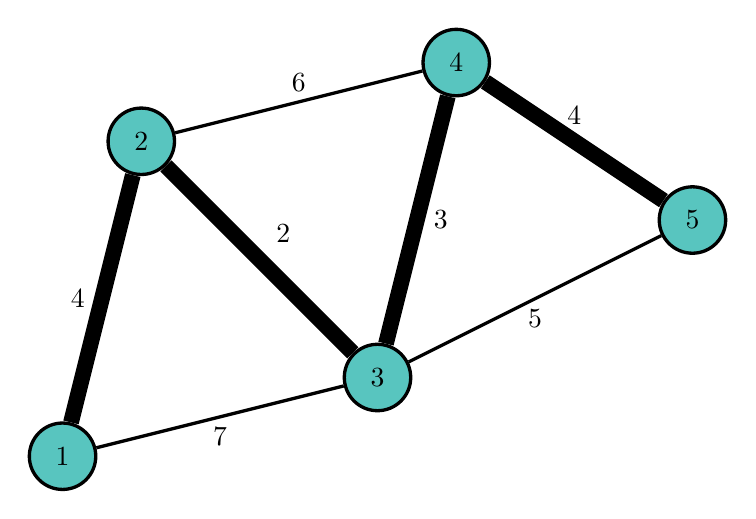
\begin{tikzpicture}[very thick,edge from parent/.style={draw,<-},level/.style={sibling distance=30mm/#1}]
\draw (0, 0) node [vertex] (v1) {1};
\draw (1, 4) node [vertex] (v2) {2};
\draw (4, 1) node [vertex] (v3) {3};
\draw (5, 5) node [vertex] (v4) {4};
\draw (8, 3) node [vertex] (v5) {5};
\draw[line width=2mm] (v1) -- (v2) node[midway, left] {4};
\draw[line width=2mm] (v2) -- (v3) node[midway, above right] {2};
\draw (v1) -- (v3) node[midway, below] {7};
\draw (v2) -- (v4) node[midway, above] {6};
\draw[line width=2mm] (v3) -- (v4) node[midway, right] {3};
\draw (v3) -- (v5) node[midway, below] {5};
\draw[line width=2mm] (v4) -- (v5) node[midway, above] {4};
\end{tikzpicture}
\end{center}

\subsection{Prim}

Prim's algorithm for finding the minimum spanning tree is very similar to Dijkstra's algorithm for finding the shortest path. Like Dijkstra, it iteratively adds a new vertex at a time to build a tree. The only difference is $dist(v)$ stores the shortest distance from \textit{any} visited node instead of the source.

\begin{algorithm}[H]
\caption{Prim}
\begin{algorithmic}
\ForAll{vertices $v$}
	\State $dist(v) \gets \infty$
	\State $visited(v) \gets 0$
    \State $prev(v) \gets -1$
\EndFor
\State $dist(src) \gets 0$
\While{$\exists v$ s.t. $visited(v)=0$}
	\State $v \equiv v$ s.t. $visited(v)=0$ with min $dist(v)$
    \State $visited(v) \gets 1$
	\ForAll{neighbors $u$ of $v$}
    	\If{$visited(u) = 0$}
			\If{$weight(v, u) < dist(u)$}
				\State $dist(u) \gets weight(v, u)$
   	        	\State $prev(u) \gets v$
			\EndIf
        \EndIf
    \EndFor
\EndWhile
\end{algorithmic}
\end{algorithm}

The proof of correctness is left as an exercise. The complexity of this algorithm depends on how the minimum unvisited vertex is calculated. Using the same approaches as Dijkstra, we can achieve $O(V^2)$ or $O(E \log{V})$.

\subsection{Kruskal}

While Prim greedily adds vertices to the tree, Kruskal's algorithm greedily adds edges. It iterates over all the edges, sorted by weight. We need to watch out for adding a cycle, breaking the tree structure, which means we need to keep track of each vertex's connected component. If an edge connects two vertices from the same connected component, we don't want to add it to our tree. However, we have a union-find algorithm that works perfectly for this.

\begin{algorithm}[H]
\caption{Kruskal}
\begin{algorithmic}
\ForAll{edges $(u,v)$ in sorted order}
	\If{$\Call{Find}{u} \not= \Call{Find}{v}$}
		\State add $(u,v)$ to spanning tree
		\State $\Call{Union}{u,v}$
	\EndIf
\EndFor
\end{algorithmic}
\end{algorithm}

This algorithm requires a sort of the edges and thus has complexity $O(E \log{E}) = O(E \log{V})$.

\section{Eulerian Tour}

An \textit{Eulerian tour} of a graph is a path that traverses every edge exactly once. If the tour ends exactly where it started, it is called an \textit{Eulerian circuit}. A graph has an Eulerian circuit if it is connected and every vertex has even degree. A graph has an Eulerian path if it is connected and all vertices but exactly two have even degrees. The mathematical proofs for these graph properties hinge on the idea that removing a cycle from the graph maintains the Eulerian property. We construct an Eulerian tour by appealing to this idea.

\begin{algorithm}[H]
\caption{Eulerian Tour}
\begin{algorithmic}
\Function{FindTour}{$v$}
\While{$v$ has a neighbor $u$}
	\State delete edge $(v,u)$
	\State \Call{FindTour}{$u$}
	\Comment{\Call{FindTour}{$u$} must trace a circuit back to $v$}
\EndWhile
\State add $v$ to tour
\EndFunction
\end{algorithmic}
\end{algorithm}

It is not preferable to use the run-time stack; we can use our own stack if necessary.

If the graph contains an Eulerian circuit, we call this function on any vertex we like. If it contains an Eulerian path, we call this function on one of the vertices with odd degree.

\section{Maximum Flow}

We are given a directed graph with weighted edges, a source node, and a sink node. A \textit{flow} is sent from the source to the sink. Each edge weight represents the maximum capacity of that edge. For every node besides the source and the sink node, total flow in is equal to total flow out. We can think of a flow network as a series of pipes through which water travels from an entrance to an exit in the network. The edge capacities represent pipe thickness. At any node, the total rate at which water enters the node must equal the total rate at which it exits the node, and along any path, the rate at which water flows is bottlenecked by the thinnest pipe.

More formally, for a graph $G(V,E)$, where $c(u,v)$ represents the capacity of the edge from $u$ to $v$, the flow $f(u,v)$ from a source $s$ to a sink $t$ satisfies

\begin{align*}
f(u,v) &\le c(u,v) \forall (u,v) \in E \\
f(u,v) &= -f(v,u) \forall (u,v) \in E \\
\sum_{v \in V} f(u,v) &= 0 \forall u \in V \setminus \{s,t\} \\
\sum_{v \in V} f(s,v) &= \sum_{v \in V} f(v,t) = |f|,
\end{align*}

where $|f|$ represents the total flow from the source to the sink.

A \textit{maximum flow} is one that maximizes the total flow $|f|$ from $s$ to $t$, or in our example, maximizes the rate at which water can flow through our network.

We'll also define the residual capacity $c_f(u,v) = c(u,v) - f(u,v)$. Note that $c_f(u,v) \ge 0$ by the conditions imposed on $f$. The residual capacity of an edge represents how much capacity is left after a certain amount of flow has already been sent. We therefore have the residual graph $G_f(V,E_f)$, where $E_f$ is the graph of residual edges, or all edges $(u,v) \in V^2$ satisfying $c_f(u,v) > 0$.

A natural approach to ``solving'' this problem would be to simply greedily add flow.

Find a path from the source to the sink in which all the edges have positive weight in the residual graph. Send flow along this path; that is, find the max flow across this path, which is the minimum weight of any edge on this particular path. Call this value $cap$. Then subtract $cap$ from the residual capacity of every edge in the path. We repeat, and this is guaranteed to terminate since on any given move, we remove an edge from our residual graph.

What is wrong with our greedy approach? Consider the following graph:

\begin{center}
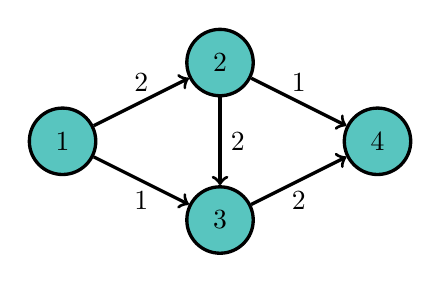
\begin{tikzpicture}[very thick,level/.style={sibling distance=70mm/#1}]
\draw (0, 0) node [vertex] (n1) {1};
\draw (2, 1) node [vertex] (n2) {2};
\draw (2, -1) node  [vertex] (n3) {3};
\draw (4, 0) node [vertex] (n4) {4};
\draw[->] (n1) -- (n2) node[midway, above] {2};
\draw[->] (n2) -- (n3) node[midway, right] {2};
\draw[->] (n3) -- (n4) node[midway, below] {2};
\draw[->] (n2) -- (n4) node[midway, above] {1};
\draw[->] (n1) -- (n3) node[midway, below] {1};
\end{tikzpicture}
\end{center}

The max flow from vertex 1 to vertex 4 is 3, but greedy gives only 2. This is because the best possible single path from the source to the sink may not be included the best possible overall flow.

\subsection{Ford-Fulkerson}

We somehow need a way to fix the inclusion of any suboptimal paths in our greedy approach, or to ``send flow back'' in case we sent it through a suboptimal path. We do this by introducing the \textit{reverse edge} to our residual graph.

Find a path from the source to the sink in which all the edges have positive weight in the residual graph. Find the max flow across this path, which is the minimum weight of any edge on this particular path. Call this value $cap$. Then subtract $cap$ from the residual capacity of every edge along the path and \textit{increment the residual capacity of the reverse edge} (the edge connecting the same two vertices but running in the opposite direction) by $cap$. We call this operation on the path \textit{augmenting the path}. We simply choose an augmenting path until no such paths exist.

\begin{algorithm}[H]
\caption{Ford-Fulkerson}
\begin{algorithmic}
\Function{AugmentPath}{path $p=\{v_i\}_{i=1}^m$, where $(v_i,v_{i+1}) \in E_f$, $v_1=s$, $v_m=t$}
\State $cap \gets \min_{i=1}^{m-1}(c_f(v_i,v_{i+1}))$
\For{$i \equiv 1, m-1$}
	\State $f(v_i,v_{i+1}) \gets f(v_i,v_{i+1}) + cap$
	\State $c_f(v_i,v_{i+1}) \gets c_f(v_i,v_{i+1}) + cap$
	\State $f(v_{i+1},v_i) \gets f(v_{i+1},v_i) - cap$
	\State $c_f(v_{i+1},v_i) \gets c_f(v_{i+1},v_i) + cap$
	\Comment incrementing reverse edge
\EndFor
\EndFunction
\Function{MaxFlow}{$G(V,E)$, $s,t \in V$}
	\ForAll{$(u,v) \in V^2$}
		\State $f(u,v) \gets 0$
		\State $c_f(u,v) \gets c(u,v)$
	\EndFor
	\State $|f| \gets 0$
	\While{$\exists p=\{v_i\}_{i=1}^m$, where $(v_i,v_{i+1}) \in E_f$, $v_1=s$, $v_m=t$}
		\State $cap \gets \min_{i=1}^{m-1}(c_f(v_i,v_{i+1}))$
		\State $|f| \gets |f| + cap$
		\State \Call{AugmentPath}{$p$}
	\EndWhile
	\Return $|f|$
\EndFunction
\end{algorithmic}
\end{algorithm}

The difference between this algorithm and the greedy approach from earlier is that the paths we now allow may run along a reverse path, essentially undoing any suboptimal flow from earlier. These more general paths in our residual graph are called \textit{augmenting paths}.

This algorithm is guaranteed to terminate for graphs with integral weights. Its performance is bounded by $O(Ef)$, where $f$ is the maximum flow and $E$ is the number of edges, as finding a path from $s$ to $t$ takes $O(E)$ and increments the total flow $f$ by at least 1. The concept of removing edges can't be used to produce a stricter bound because while an edge in one direction may be removed from the residual graph, doing so creates an edge in the other direction.

In its crudest form, Ford-Fulkerson does not specify on which path to push flow if multiple paths exist. It simply states that as long as such a path exists, push flow onto it. In addition to being slow, Ford-Fulkerson, as it is stated, is not guaranteed to terminate for graphs with non-integral capacities. In fact, it might not even converge to the maximum flow for irrational capacities. However, these problems can be fixed by simply specifying how the algorithm chooses the next path on which to push flow. Nonetheless, the Ford-Fulkerson algorithm is formulated beautifully mathematically and such is useful from a math perspective, as we will see with the Max-Flow Min-Cut Theorem.

\subsection{Max-Flow Min-Cut Theorem}

On a graph $G(V,E)$, an \textit{s-t cut} $C=(S,T)$ splits the partitions $V$ into $S$ and $T$ satisfying $s \in S$ and $t \in T$. The \textit{cut-set} of $C$ is the set of edges $\{(u,v) \in E : u \in S, v \in T\}$. The \textit{capacity} of an s-t cut is given by

\[c(S,T) = \sum_{(u,v) \in S \times T}c(u,v).\]

A \textit{minimum cut} is an s-t cut that minimizes $c(S,T)$.

A cut represents a set of edges that, once removed, separates $s$ from $t$. A minimum cut is therefore a set of edges that does this but minimizes the total capacity of the edges necessary to disconnect $s$ from $t$.

The max-flow min-cut theorem states that the maximum value of any s-t flow is equal to the minimum capacity of any s-t cut.

First, the capacity of any cut must be at least the total flow. This is true by contradiction. Any path from $s$ to $t$ has an edge in the cut-set, so therefore any flow from $s$ to $t$ is upper bounded by the capacity of the cut. Therefore, we need only construct one flow and one cut such that the capacity of the cut is equal to the flow.

We consider the residual graph $G_f$ produced at the completion of the Ford-Fulkerson augmenting path algorithm.\footnote{If you're concerned that the Ford-Fulkerson algorithm will never terminate, there always exists a sequence of paths chosen such that it will. Edmonds-Karp is one example that always terminates.} Let the set $S$ be all nodes reachable from $s$ and $T$ be $V \setminus S$. We wish to show that $C=(S,T)$ is a cut satisfying $|f|=c(S,T)=\sum_{(u,v) \in S \times T} c(u,v)$. This is true when the following is satisfied:

\begin{enumerate}

\item
All edges $(u,v) \in S \times T$ are fully saturated by the flow. That is, $c_f(u,v) = 0$.

\item
All reverse edges $(v, u) \in T \times S$ have zero flow. That is, $f(v,u) = 0$, or $c_f(v,u) = c(v,u)$.

\end{enumerate}

The first condition is true by the way we constructed $S$ and $T$, as if there existed a $(u,v)$ where $c_f(u,v) > 0$, then $v$ is accessible to $s$ and ought to have been in $S$.

The second condition is true by the way the Ford-Fulkerson algorithm constructed reverse edges. If net flow was sent from $v$ to $u$, then a reverse edge was constructed from $u$ to $v$, so again, $v$ is accessible to $s$, which is a contradiction.

Therefore, we have the flow
\[|f|=\sum_{(u,v) \in S \times T} c(u,v) - \sum_{(v,u) \in T \times S} 0 = c(S,T),\]
so we constructed a flow and a cut such that the flow $|f|$ is equal to the cut capacity $c(S,T)$, and we are done.

\subsection{Refinements of Ford-Fulkerson}

As stated earlier, Ford-Fulkerson is limited by not specifying on which path to push flow. There are many algorithms that resolve this issue in different ways.

\subsubsection{Edmonds-Karp}

Edmonds-Karp fixes the problem by simply choosing the augmenting path of shortest unweighted length. This can be done easily using a BFS.

\begin{algorithm}[H]
\caption{Edmonds-Karp}
\begin{algorithmic}
\Function{ChoosePath}{$G_f(V,E_f)$, $s,t \in V$}
	\Comment{BFS}
	\State $visited(v)$ denotes $v$ has been added to queue
	\State $prev(v)$ denotes vertex preceding $v$ in BFS
	\State push $s$ on queue $Q$
	\State $visited(s) \gets 1$
	\While{$Q$ is not empty}
		\State $u \gets $ top of $Q$
		\ForAll{neighbors $v$ of $u$ in $G_f$ where $visited(v)=0$}
			\State push $v$ on $Q$
			\State $visited(v) \gets 1$
			\State $prev(v) \gets u$
		\EndFor
	\EndWhile
	\State pointer $curr \gets t$
	\While{$curr \not= s$}
		\State add $curr$ to beginning of path $p$
		\State $curr \gets prev(curr)$
	\EndWhile
	\State add $s$ to beginning of $p$
	\State \Return $p$
\EndFunction
\Function{MaxFlow}{$G(V,E)$, $s,t \in V$}
	\ForAll{$(u,v) \in V^2$}
		\State $f(u,v) \gets 0$
		\State $c_f(u,v) \gets c(u,v)$
	\EndFor
	\State $|f| \gets 0$
	\While{$t$ can be reached from $s$}
		\State $p \gets \Call{ChoosePath}{G_f,s,t}$
		\State $cap \gets \min_{i=1}^{m-1}(c_f(v_i,v_{i+1}))$
		\State $|f| \gets |f| + cap$
		\State \Call{AugmentPath}{$p$}
	\EndWhile
	\Return $|f|$
\EndFunction
\end{algorithmic}
\end{algorithm}

The BFS is clearly $O(E)$. To complete our analysis, we must somehow bound the number of times we need to perform the BFS. To do this, we'll look at what pushing flow on a path does to our residual graph; in particular, how it affects our BFS traversal tree. Note that each vertex is on some level $i$ in the BFS tree, characterized by the distance from the source $s$. For example, $L_0 = \{s\}$, $L_1$ contains all the neighbors of $s$, $L_2$ contains neighbors of neighbors not in $L_0$ or $L_1$, and so on.

We first claim that the level of any vertex in the graph is nondecreasing following an augment on a path $p$. If the augment saturates an edge, it may remove it from $G_f$, which cannot decrease the distance of any vertex from $s$. If the augment creates an edge $e=(u,v)$, that means we sent flow from $v$ to $u$ on the path $p$. Therefore, if $v$ was originally level $i$, $u$ must have been level $i+1$. The level of $u$ does not change by adding $(u,v)$, and the level of $v$ can either be $i$ or $i+2$, depending on whether edge $(v,u)$ was deleted in the process. Either way, the level of all vertices is nondecreasing.

Now consider the bottleneck edge $e=(u,v)$ of an augmenting path $p$, where the level of $u$ is $i$ and the level of $v$ is $i+1$. The push operation deletes the edge $e$, but the level of $v$ must stay at least $i+1$. Now for the edge $e$ to reappear in the graph $G_f$, flow must have been sent on the reverse edge $e'=(v,u)$ on some augmenting path $p'$. But on path $p'$, $u$ comes after $v$, which must be at least level $i+1$. Therefore, $u$ must be at least level $i$. But since the maximum level of a node that is connected to $s$ is $V-1$, an edge $e$ can only be chosen as the bottleneck edge $\frac{V}{2}$ times, or $O(V)$.

There are $E$ edges, each of which can be the bottleneck edge for $O(V)$ different augmenting paths, each of which takes $O(E)$ to process. Therefore, the Edmonds-Karp algorithm runs in $O(VE^2)$.

\subsubsection{Dinic}

Dinic's algorithm is another refinement of Ford-Fulkerson.

\subsection{Push-Relabel}

Unfortunately, even the much-improved bounds of the $O(VE^2)$ Edmonds-Karp are admittedly bad. While the push-relabel method for solving the max flow problem does not have the fastest theoretical bounds, two of its implementations have complexities $O(V^3)$ and $O(V^2\sqrt{E})$ and are among the fastest in practice.

\subsubsection{Generic Push-Relabel}

Ford-Fulkerson and its variants all deal with global augmentations of paths from $s$ to $t$. Push-relabel takes a different perspective, introducing the concept of a \textit{preflow} and a \textit{height} to make local optimizations that ultimately result in the maximum flow.

A preflow maintains the same properties as a flow but modifies the conservation of flow condition. Instead of total flow in equalling total flow out, flow in must be at least, and therefore can exceed, flow out. We denote the difference between flow in and flow out as the \textit{excess} $e(v)$.

\begin{align*}
f(u,v) &\le c(u,v) \forall (u,v) \in E \\
f(u,v) &= -f(v,u) \forall (u,v) \in E \\
e(v) = \sum_{u \in V} f(u,v) &\ge 0 \forall v \in V \setminus \{s\} \\
e(s) &= \infty.
\end{align*}

The definitions of the residual capacity $c_f(u,v)$, edge set $E_f$, and graph $G_f$ are the same as they were defined before, except with a preflow $f$ instead of a normal flow.

We call a vertex $v \in V \setminus \{s, t\}$ \textit{active} if $e(v) > 0$. Therefore, a vertex besides the source or sink is active if more flows into the vertex than flows out. $s$ and $t$ are \textit{never} active. A preflow with no active vertices is simply a flow, at which point the excess of the sink $e(t)$ represents the value $|f|$ of the flow.

We can \textit{push} flow from a node $u$ to a node $v$ by moving as much of the excess $e(u)$ to $v$ as the capacity of the edge $c_f(u,v)$ will allow.

\noindent \begin{minipage}{\textwidth}
\begin{algorithmic}
\Function{Push}{edge $(u,v)$}
	\State $\delta \gets \min(e(u), c_f(u,v))$
	\Comment $c_f(u,v) = c(u,v) - f(u,v)$
	\State $f(u,v) \gets f(u,v) + \delta$
	\State $f(v,u) \gets f(v,y) - \delta$
	\State $e(u) \gets e(u) - \delta$
	\State $e(v) \gets e(v) + \delta$
\EndFunction
\end{algorithmic}
\end{minipage}

The idea of the push-relabel algorithm is to first push as much preflow as possible through local optimizations in the direction the sink. When a node can no longer push flow to the sink, it pushes the excess back towards the source to turn the preflow into a flow.

However, the difficulty here lies in establishing this sense of ``direction'' from the source to the sink. Remember that we simply push preflow along a single edge in the graph at a time, not along a whole path. Moving flow from the source to the sink along a path that goes from the source to the sink is easy; moving flow from the source to the sink through local pushes without the knowledge of the graph structure as a whole is indeed a much harder problem.

To resolve this issue, we introduce a \textit{label} to each of the nodes. The label $h(u)$ represents the ``height'' of $u$. In real life, water flows from higher to lower ground. We want $s$ to represent that high ground and $t$ to represent the low ground. As we push preflow from $s$ to $t$, vertices along the way represent height values between those of $s$ and $t$. However, eventually we have to push preflow back to handle both excesses in flow and suboptimal previous pushes, \`{a} la Ford-Fulkerson, but this contradicts the concept of height as we can't flow both downhill and uphill. Therefore, we'll need to be able to \textit{relabel} a node, changing the height $h(u)$ to something that allows preflow to flow back towards $s$. We will relabel $h$ in a systematic way that allows us to direct the preflow through the graph.

For this labeling to be useful for us, we'll need to impose some more constraints that must be satisfied no matter how we change the graph $G_f$ or the height function $h$.

\begin{align*}
h(u) &\le h(v) + 1 \forall (u,v) \in E_f \\
h(s) &= |V| \\
h(t) &= 0.
\end{align*}

What does this mean? For our algorithm, we can push preflow along the edge from $u$ to $v$ only if $c_f(u,v) > 0$ and $h(u) > h(v)$, so $h(u) = h(v) + 1$. We call such an edge $(u,v) \in E_f$ \textit{admissible}. Furthermore, for all vertices $v$ that can reach $t$ in $E_f$, $h(v)$ represents the lower bound for the length of any unweighted path from $v$ to $t$ in $G_f$, and for all vertices that cannot reach $t$, then $h(v)-|V|$ is a lower bound for the unweighted distance from $s$ to $v$.

$t$ will always represent the lowest node, so $h(t)=0$ is a natural constraint. We'll first set the preflow values of all vertices $v$ that can be immediately reached from $s$ to $c(s,v)$, saturating all the out-edges of $s$. For any vertex $v$ from which $t$ can be reached, $h(v)$ represents the lower bound of the unweighted distance to $t$ from $v$ in the residual graph.

We want $h(s)$ to be a number large enough that will indicate that $s$ has been disconnected to $t$, as we have already sent as much preflow possible from $s$ in the direction of $t$ by saturating all outgoing edges. Therefore, setting $h(s)=|V|$ is also natural. Since $h(s)$ represents the lower bound of the distance from $s$ to $t$ in $G_f$, and there are no paths from $s$ to $t$ in the residual graph, $|V|$ is a natural choice, since the longest possible path is $|V|-1$.

Furthermore, we don't want any preflow sent back to $s$ from a vertex $v$ unless it is impossible to send any more preflow from $v$ to $t$. If preflow is pushed from $v$ to $s$, then $h(v) = |V| + 1$. If there existed a path $v$ to $t$ such that every edge is admissible, the path must have $|V| + 2$ vertices. This is true because for any two consecutive vertices $v_i,v_{i+1}$ in the path, $h(v_i) = h(v_{i+1}) + 1$, but no path can have $|V|+2$ distinct vertices.

This leads to the fact that the only nodes that can possibly continue to contribute to the final flow are active vertices $v$ for which $h(v) < |V|$. A node with height at least $|V|$ does not have a valid path to $t$, and a node that is not active doesn't have any excess flow to push.

Now that I've explained the general idea behind the labeling constraints, it's time to actually describe what our relabeling process is. At first, the labels of all vertices besides the source start at 0. We only relabel a node $v$ if it is active (therefore, it has excess flow it needs to push; $e(u) > 0$) but has no admissible out-edges in $G_f$ (so it has no adjacent vertex on which it can push that excess flow). If a node has no admissible out-edges in $G_f$, every neighbor of $u$ has a height label at least equal to $h(u)$. When we relabel a node, we always then \textit{increase} the value of $h(u)$ to the least value where it can push flow onto another node.

\noindent \begin{minipage}{\textwidth}
\begin{algorithmic}
\Function{Relabel}{vertex $u$}
		\State $h(u) \gets \min_{v | (u,v) \in E_f}(h(v)) + 1$
		\Comment $(u,v) \in E_f \iff c_f(u,v) = c(u,v) - f(u,v) > 0$
\EndFunction
\end{algorithmic}
\end{minipage}

Since we take the minimum height of all neighbors in the graph, we first try adjusting the height of $u$ so that we can push flow from $u$ to its neighbors that can possibly still reach $t$; that is, neighbors $v$ satisfying $h(v) < |V|$. Once we try all these neighbors, we then increase the height of $u$ to begin to push flow back towards $s$. We can always find such an edge, as any preflow pushed onto $u$ must have also incremented the reverse edge from $u$ back towards $s$.

Note that neither pushing on a admissible edge nor relabeling a vertex with no admissible out-edges changes the fact that $h$ remains a valid labeling function.

The generic push-relabel algorithm simply pushes and relabels vertices until there are no active vertices and the preflow becomes a flow. This algorithm works because throughout the process, $h$ remained a valid height function, and at the end, the preflow was converted into a flow. Since $h(s) = |V|$ and $h(t) = 0$, there is no augmenting path from $s$ to $t$, so our flow is maximal.

\begin{algorithm}[H]
\caption{Push-Relabel (Generic)}
\begin{algorithmic}
\Function{Push}{edge $(u,v)$}
	\If{$e(u) > 0$ and $h(u) = h(v) + 1$}
		\Comment push condition
		\State $\delta \gets \min(e(u), c_f(u,v))$
		\Comment $c_f(u,v) = c(u,v) - f(u,v)$
		\State $f(u,v) \gets f(u,v) + \delta$
		\State $f(v,u) \gets f(v,y) - \delta$
		\State $e(u) \gets e(u) - \delta$
		\State $e(v) \gets e(v) + \delta$
	\EndIf
\EndFunction
\Function{Relabel}{vertex $u$}
	\If{$u \not= s,t$ and $e(u)>0$ and $h(u) \le h(v) \forall v | (u,v) \in E_f$}
		\Comment relabel condition
		\State $h(u) \gets \min_{v | (u,v) \in E_f}(h(v)) + 1$
		\Comment $(u,v) \in E_f \iff c_f(u,v) = c(u,v) - f(u,v) > 0$
	\EndIf
\EndFunction
\Function{MaxFlow}{$G(V,E)$, $s,t \in V$}
	\ForAll{$v \in V \setminus \{s\}$}
		\Comment initialize excess
		\State $e(v) \gets 0$
	\EndFor
	\State $e(s) \gets \infty$
	\ForAll{$(u,v) \in V^2$}
		\Comment initialize preflow
		\State $f(u,v) \gets 0$
	\EndFor
	\ForAll{neighbors $v \not= s$ of $s$}
		\Comment saturate edges to all neighbors of $s$
		\State $f(s,v) \gets c(s,v)$
		\State $f(v,s) \gets -c(s,v)$
		\State $e(v) \gets c(s,v)$
	\EndFor
	\ForAll{$v \in V \setminus \{s\}$}
		\Comment preflow now has valid height function; initialize height
		\State $h(v) \gets 0$
	\EndFor
	\State $h(s) \gets |V|$
	\While{we can still \Call{Push}{} or \Call{Relabel}{}}
		\State \Call{Push}{} or \Call{Relabel}{}
	\EndWhile
	\State \Return $e(t)$
	\Comment $e(t)=|f|$
\EndFunction
\end{algorithmic}
\end{algorithm}

We can argue that this algorithm runs in $O(V^2E)$, which is already an improvement from Edmonds-Karp. However, just as Ford-Fulkerson could be sped up by specifying which augmenting paths to choose, we can do the same with the push-relabel algorithm, speeding it up by specifying a systematic method to choose an edge to push or a vertex to relabel.

\subsubsection{Discharge}

We first describe an auxiliary operation. For each vertex $u$, we'll need a way to visit in- and out-neighbors of $u$ in a static cyclic order. This is easy with just a pointer; for vertex $u$, we'll call that pointer $curr(u)$. When the pointer passes through every element in the list of neighbors, we'll just reset it back to the first element.

\noindent \begin{minipage}{\textwidth}
\begin{algorithmic}
\Function{Discharge}{vertex $u$}
	\While{$e(u)>0$}
		\Comment{perform an operation as long as $u$ is active}
		\If{$curr(u)$ is at end of list of neighbors}
			\State \Call{Relabel}{$u$}
			\State reset $curr(u)$
		\Else
			\If{$(u,curr(u))$ is an admissible edge}
				\State \Call{Push}{$(u,curr(u))$}
			\Else
				\State move $curr(u)$ to next neighbor of $u$
			\EndIf
		\EndIf
	\EndWhile
\EndFunction
\end{algorithmic}
\end{minipage}

\subsubsection{FIFO Selection}

FIFO selection simply maintains a list of active vertices in a FIFO queue. We pop off the first vertex in the queue and discharge it, adding any newly-activated vertices to the end of the queue. This runs in $O(V^3)$.

\subsubsection{Highest Label Selection}

Highest label selection discharges the active vertex with the greatest height. This runs in $O(V^2\sqrt{E})$.

\subsubsection{Improvements with Heuristics}

Heuristics are meant to help relabel vertices in a smarter way. Bad relabelings are the slowest part of the algorithm, and improving the process can speed up max flow.

The \textit{gap heuristic} takes advantage of ``gaps'' in the height function. Since a path of admissible edges consists of vertices whose heights decrease by exactly 1, the presence of a gap in height precludes the possibility of such a path. If there exists a value $h'$ such that no vertex $v$ exists such that $h(v)=h'$, then for every vertex $v$ satisfying $h' < h(v) < |V|$, $v$ has been disconnected from $t$, so we can immediately relabel $h(v)=|V| + 1$.

The \textit{global relabeling heuristic} performs a backwards BFS from $t$ every now and then to compute the heights of the vertices in the graph exactly.

Some dude on Codeforces\footnote{\url{http://codeforces.com/blog/entry/14378}} didn't have much luck improving performance with the global relabeling heuristic. I'd suggest sticking to the gap heuristic only.

\subsection{Other Problems with Flow Solutions}

\subsubsection{Bipartite Matching}

\subsubsection{Edge-Disjoint Paths}



\chapter{Computational Geometry}

For actual geometry problems, and not graph theory problems hiding in the plane.

I'm too lazy to actually write this section right now so here are some useful links from the USACO Training Pages.

\url{https://www.dropbox.com/s/nqzk63bjby1iaq9/Computational\%20Geometry.pdf?dl=0}

\url{https://www.dropbox.com/s/ykf65dk6sefb6zk/2-D\%20Convex\%20Hull.pdf?dl=0}

These essentially cover anything I would want to say in this chapter anyway, so I'll likely fill this chapter out last.

\section{Basic Tools}

\subsubsection{Cross Product}

\subsubsection{Dot Product}

\subsubsection{$\tan^{-1}$, \texttt{atan2}}

\section{Formulas}

\subsection{Area}

\subsection{Distance}

\subsection{Configuration}

\subsection{Intersection}

\section{Convex Hull}

\section{Sweep Line}

Oftentimes when trying to solve geometry problems, or combinatorial problems that we give a geometric interpretation, we have something that involves one or two dimensions. If this is difficult to deal with directly, we can use a sweep line to reduce the dimension of the problem.

Sweeplines are best explained with an example. Suppose we're given several intervals on the number line, and we want to find the length of their union. If we wanted to, we could use a segment tree with lazy propagation to insert the intervals and calculate the total length. However, a sweep line gives us a much easier approach. Imagine a vertical beam of light sweeping from $-\infty$ to $\infty$ on the number line. At any given time, we keep track of the number of intervals that are hit by this beam. This takes the problem from one dimension to zero dimensions. Our answer is then the length over which our beam hit a positive number of intervals.

Our implementation of a sweep line simulates this process. If we sort the endpoints of our intervals by their positions on the number line, we can simply increment our counter each time we encounter a ``start'' endpoint and decrement our counter each time we encounter an ``end'' endpoint. We can look at the regions between consecutive endpoints, and add to our result if our counter is positive in that region.

\begin{center}\begin{tikzpicture}
  \coordinate (A) at (2,1);
  \coordinate (B) at (6,1);
  \coordinate (C) at (0,2);
  \coordinate (D) at (3,2);
  \coordinate (E) at (5,2);
  \coordinate (F) at (7,2);
  \coordinate (G) at (1,3);
  \coordinate (H) at (5,3);
  \draw[fill] (A) circle [radius=2pt];
  \draw[fill] (B) circle [radius=2pt];
  \draw[fill] (C) circle [radius=2pt];
  \draw[fill] (D) circle [radius=2pt];
  \draw[fill] (E) circle [radius=2pt];
  \draw[fill] (F) circle [radius=2pt];
  \draw[fill] (G) circle [radius=2pt];
  \draw[fill] (H) circle [radius=2pt];
  \draw[ultra thick] (A) -- (B);
  \draw[very thick] (C) -- (D);
  \draw[very thick] (E) -- (F);
  \draw[ultra thick] (G) -- (H);

  \draw[<->] (-1,0) -- (8,0);
  \foreach \x in {0, 1, 2, 3, 4, 5, 6, 7}
  \draw[shift={(\x,0)}] (0,3pt) -- (0,-3pt);

  \draw[<->, very thick, dashed, color=red] (3.75,-1) -- (3.75,4);
\end{tikzpicture}\end{center}

One other way to interpret sweep lines is to consider time as the dimension we sweep along. For the example above, this would mean that each interval appears and then disappears on our beam, existing only when the time is between its endpoints. Although time may not seem useful for our one dimensional problem, this type of thinking helps in higher dimensions. 

Most sweep lines that you use won't be as simple as this. Sweepline problems usually involve reducing a two dimensional problem to a one dimensional problem and require maintaining data structures such as BBSTs or segment trees along that dimension. This technique also generalizes to higher dimensions---to solve a three dimensional problem, we can sweep along one dimension and use two dimensional data structures to maintain the other two dimensions.

To finish, let's go over another example, Cow Rectangles from USACO 2015 January:

\texttt{
\fontdimen2\font=0.4em% interword space
\fontdimen3\font=0.2em% interword stretch
\fontdimen4\font=0.1em% interword shrink
\fontdimen7\font=0.1em% extra space
\hyphenchar\font=`\-% allowing hyphenation
The locations of Farmer John's $N$ cows ($1 \le N \le 500$) are described by distinct points in the 2D plane. The cows belong to two different breeds: Holsteins and Guernseys. Farmer John wants to build a rectangular fence with sides parallel to the coordinate axes enclosing only Holsteins, with no Guernseys (a cow counts as enclosed even if it is on the boundary of the fence). Among all such fences, Farmer John wants to build a fence enclosing the maximum number of Holsteins. And among all these fences, Farmer John wants to build a fence of minimum possible area. Please determine this area. A fence of zero width or height is allowable.}

The first observation we should make is that we want a Holstein on every side of the fence. Otherwise, we would be able to decrease the area of our fence without decreasing the number of Holsteins. Even with our observation, this problem still seems hard to deal with. We can make it easier by adding another constraint: Suppose we knew which Holstein was on the leftmost boundary of our fence. Since we added the constraint to the $x$-dimension, we naturally want to figure out where our rightmost Holstein is next. We can do this with a sweep line moving to the right.

The reason we want a sweep line here is because for any given rightmost cow, we want to know information about the Guernseys and Holsteins inbetween. With a sweep line, we can collect and maintain all this data by processing the cows from left to right. For example, whenever we see a Guernsey, we have to limit the $y$-coordinates that our Holsteins can take. And whenever we see a Holstein, we have to consider this Holstein as our rightmost cow and also store it in case we include it in a fence later on.

What remains is to find an appropriate data structure to track all this. A set data structure (STL set or Java TreeMap) turns out to be enough. We can insert the Holsteins, sorted by $y$-coordinate, and delete one whenever any rectangle bounded by that Holstein, the leftmost Holstein, and our sweep line includes a Guernsey. Thus we take $O(n \log n)$ time to sweep, giving us an $O(n^2 \log n)$ solution overall.

This type of analysis is pretty representative of sweep line problems. Whether you're given rectangles, line segments or even polygons, you want to think about how you can reduce the dimension and obtain a tractable problem. Note that sweep lines don't always have to move along some axis. Radial sweep lines (sweeping by rotating) and sweeping at an angle (rotating the plane by $45^\circ$) also work. 


\chapter{Complex Ideas and Data Structures}

Here we build on previous material to introduce more complex ideas that are useful for solving USACO Gold problems and beyond.

\section{Dynamic Programming over Subsets ($n2^n$ DP)}

We've already covered how dynamic programming can turn exponential solutions into polynomial solutions, but it can also help turn factorial solutions into exponential. Problems where the bound on $n$ is 20, for example, signal that an exponential solution is the one required. Consider the following problem:

(USACO December 2014, guard)
Farmer John and his herd are playing frisbee.  Bessie throws the
frisbee down the field, but it's going straight to Mark the field hand
on the other team!  Mark has height $H$ ($1 \le H \le 1,000,000,000$), but
there are $N$ cows on Bessie's team gathered around Mark ($2 \le N \le 20$).
They can only catch the frisbee if they can stack up to be at least as
high as Mark.  Each of the $N$ cows has a height, weight, and strength.
A cow's strength indicates the maximum amount of total weight of the
cows that can be stacked above her.  

Given these constraints, Bessie wants to know if it is possible for
her team to build a tall enough stack to catch the frisbee, and if so,
what is the maximum safety factor of such a stack.  The safety factor
of a stack is the amount of weight that can be added to the top of the
stack without exceeding any cow's strength.

We can try the $O(N!)$ brute force, trying every permutation of cows possible. However, this is far too slow. $N \le 20$ hints at an exponential solution, so we think of trying every possible subset of the cows. Given a subset $S$ of cows, the height reached is the same, so perhaps we sort the subset by strength, and put the strongest cow on the bottom. We see that this greedy approach fails: suppose that the first cow has weight 1 and strength 3 and the second cow has weight 4 and strength 2. Greedy would tell us to put the first cow on the bottom, but this fails, while putting the second cow on the bottom succeeds.

When greedy fails, the next strategy we look at is dynamic programming. To decide whether $S$ is stable, we have to find whether there exists a cow $j$ in $S$ that can support the weight of all the other cows in $S$. But how do we know whether the set $S \setminus \{j\}$ is stable? This is where dynamic programming comes in.

This leads to a $O(N 2^N)$ solution. This seems like a pain to code iteratively, but there is a nice fact about subsets: there is a cute bijection from the subsets of $\{0,1,2, \ldots, N-1\}$ to the integers from 0 to $2^N - 1$. That is, the subset $\{0,2,5,7\}$ maps to $2^0 + 2^2 + 2^5 + 2^7 = 165$ in the bijection. We call this technique \textit{masking}. We require all the subsets of $S$ to be processed before $S$ is processed, but that property is also handled by our bijection, since subtracting a power of 2 from a number decreases it. With a little knowledge of bit operators, this can be handled easily.

\noindent \begin{minipage}{\textwidth}
\begin{algorithmic}
\For{$i\gets 0, 2^N-1$}
	\Comment $i$ represents the subset $S$
	\State $dp(i) \gets -1$
	\ForAll{$j \in S$}
		\Comment $j \in S$ satisfy \texttt{i \& (1 << j) != 0}
		\State $alt \gets \min(dp(i-2^j), strength(j) - \sum_{k \in S \setminus \{j\}} weight(k))$
		\If{$dp(i) < alt$}
			\State $dp(i) \gets alt$
		\EndIf
	\EndFor
\EndFor
\end{algorithmic}
\end{minipage}

\texttt{\&} is the bitwise and function, while \texttt{<<} is the left shift operator.

\section{$\sqrt{n}$ Bucketing}

$\sqrt{n}$ bucketing is a relatively straightforward idea -- given $n$ elements $\{x_i\}_{i=1}^n$ in a sequence, we group them into $\sqrt{n}$ equal-sized buckets. The motivation for arranging elements like this is to support an operation called a \textit{range query}.

Let's take a concrete example. Suppose we want to support two operations:

\begin{itemize}
\item
$update(p, k)$ -- increment the value of $x_p$ by $k$

\item
$query(a, b)$ -- return $\sum_{i=a}^b x_i$.
\end{itemize}

Suppose we simply stored the sequence in an array. $update$ then becomes an $O(1)$ operation, but $query$ is $O(n)$.

\begin{center}
{
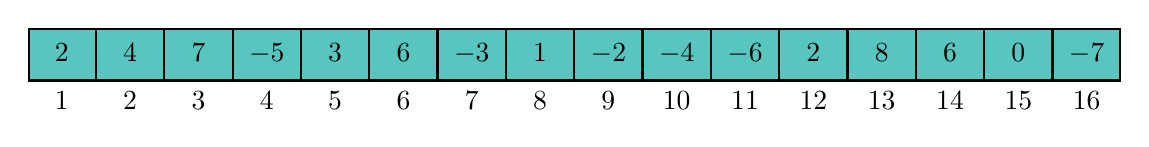
\begin{tikzpicture}[
  thick,
  myrect/.style={
    draw,
    fill=myseagreen,
    rectangle split,
    rectangle split horizontal,
    rectangle split parts=#1,
    rectangle split part align=left,
    text width=4ex,
    text centered
    }
]

\node[myrect=16]
  (array)
  {
  					\strut 2
  \nodepart{two}	\strut 4
  \nodepart{three}	\strut 7
  \nodepart{four}	\strut $-5$
  \nodepart{five}	\strut 3
  \nodepart{six}	\strut 6
  \nodepart{seven}	\strut $-3$
  \nodepart{eight}	\strut 1
  \nodepart{nine}	\strut $-2$
  \nodepart{ten}	\strut $-4$
  \nodepart{eleven}	\strut $-6$
  \nodepart{twelve}	\strut 2
  \nodepart{thirteen}	\strut 8
  \nodepart{fourteen}	\strut 6
  \nodepart{fifteen}	\strut 0
  \nodepart{sixteen}	\strut $-7$
  };
\foreach \Valor [count=\Valori from 1] in {one ,two ,three , four , five , six , seven , eight , nine , ten , eleven , twelve , thirteen , fourteen , fifteen , sixteen }
  \node[below] at (array.\Valor south) {\Valori};

\end{tikzpicture}
}
\end{center}

Another natural approach would be to store in a separate array the sum of the first $i$ terms in the sequence for every index $i$, or store the \textit{prefix sums}.

\begin{center}
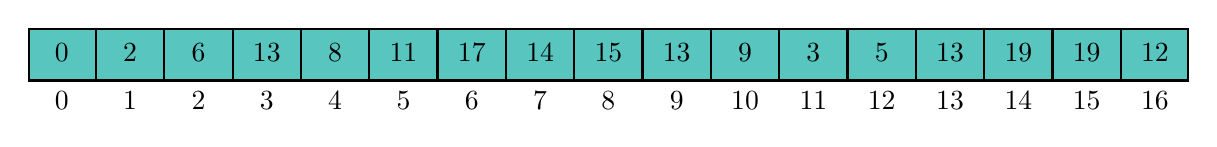
\begin{tikzpicture}[
  thick,
  myrect/.style={
    draw,
    fill=myseagreen,
    rectangle split,
    rectangle split horizontal,
    rectangle split parts=#1,
    rectangle split part align=left,
    text width=4ex,
    text centered
    }
]

\node[myrect=17]
  (array)
  {
  					\strut 0
  \nodepart{two}	\strut 2
  \nodepart{three}	\strut 6
  \nodepart{four}	\strut 13
  \nodepart{five}	\strut 8
  \nodepart{six}	\strut 11
  \nodepart{seven}	\strut 17
  \nodepart{eight}	\strut 14
  \nodepart{nine}	\strut 15
  \nodepart{ten}	\strut 13
  \nodepart{eleven}	\strut 9
  \nodepart{twelve}	\strut 3
  \nodepart{thirteen}	\strut 5
  \nodepart{fourteen}	\strut 13
  \nodepart{fifteen}	\strut 19
  \nodepart{sixteen}	\strut 19
  \nodepart{seventeen}	\strut 12
  };
\foreach \Valor [count=\Valori from 0] in {one ,two ,three , four , five , six , seven , eight , nine , ten , eleven , twelve , thirteen , fourteen , fifteen , sixteen , seventeen }
  \node[below] at (array.\Valor south) {\Valori};

\end{tikzpicture}

\end{center}

Now $query$ becomes an $O(1)$ operation, as we can simply subtract two elements in the array to answer a query. Unfortunately, $update$ becomes $O(n)$, as changing the value of an element in the beginning of the sequence forces us to change almost all the values in the prefix sum array.

We can still use this idea, though... what we are looking for is some way to group values into sums such that we only need to change a small number of the sums to $update$ and only require a small number of them to $query$.

This leads us directly to a $\sqrt{n}$ bucketing solution. Let's group the 16 elements into 4 groups.

\begin{center}
{
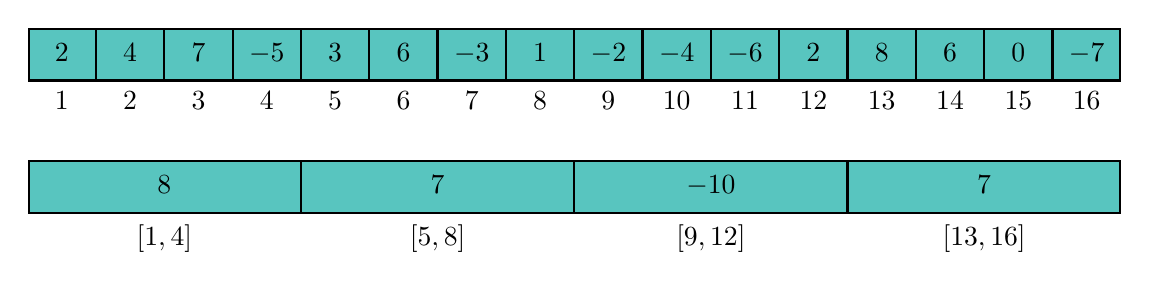
\begin{tikzpicture}[
  thick,
  myrect/.style={
    draw,
    fill=myseagreen,
    rectangle split,
    rectangle split horizontal,
    rectangle split parts=#1,
    rectangle split part align=left,
    text width=4ex,
    text centered
    }
]

\node[myrect=16]
  (array2)
  {
  					\strut 2
  \nodepart{two}	\strut 4
  \nodepart{three}	\strut 7
  \nodepart{four}	\strut $-5$
  \nodepart{five}	\strut 3
  \nodepart{six}	\strut 6
  \nodepart{seven}	\strut $-3$
  \nodepart{eight}	\strut 1
  \nodepart{nine}	\strut $-2$
  \nodepart{ten}	\strut $-4$
  \nodepart{eleven}	\strut $-6$
  \nodepart{twelve}	\strut 2
  \nodepart{thirteen}	\strut 8
  \nodepart{fourteen}	\strut 6
  \nodepart{fifteen}	\strut 0
  \nodepart{sixteen}	\strut $-7$
  };
\foreach \Valor [count=\Valori from 1] in {one ,two ,three , four , five , six , seven , eight , nine , ten , eleven , twelve , thirteen , fourteen , fifteen , sixteen }
  \node[below] at (array2.\Valor south) {\Valori};

\node[myrect=4, text width=21.2ex] [below=of array2]
  (array)
  {
  					\strut 8
  \nodepart{two}	\strut 7
  \nodepart{three}	\strut $-10$
  \nodepart{four}	\strut 7
  };

\node[below] at (array.one south) {$[1,4]$};
\node[below] at (array.two south) {$[5,8]$};
\node[below] at (array.three south) {$[9,12]$};
\node[below] at (array.four south) {$[13,16]$};
\end{tikzpicture}
}
\end{center}

We'll keep track of the total sum of each group. Now, if we want to update a value, we need to change only two values -- the value of that element in the original array and the total sum of the bucket it is in. When we query a range, we'll take advantage of the sum of the bucket when we can. Highlighted are the numbers we'll need for $query(7,15)$.

\begin{center}
{
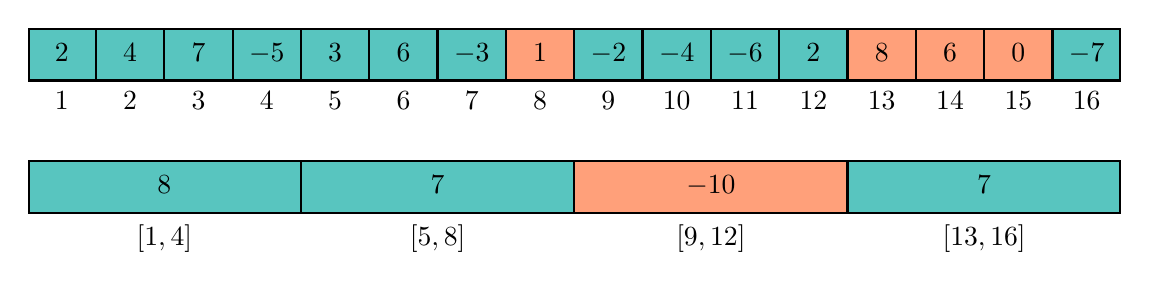
\begin{tikzpicture}[
  thick,
  myrect/.style={
    draw,
    rectangle split,
    rectangle split horizontal,
    rectangle split parts=#1,
    rectangle split part align=left,
    text width=4ex,
    text centered
    }
]

\node[myrect=16, rectangle split part fill={myseagreen, myseagreen, myseagreen, myseagreen, myseagreen, myseagreen, myseagreen, mysalmon, myseagreen, myseagreen, myseagreen, myseagreen, mysalmon, mysalmon, mysalmon, myseagreen}]
  (array2)
  {
  					\strut 2
  \nodepart{two}	\strut 4
  \nodepart{three}	\strut 7
  \nodepart{four}	\strut $-5$
  \nodepart{five}	\strut 3
  \nodepart{six}	\strut 6
  \nodepart{seven}	\strut $-3$
  \nodepart{eight}	\strut 1
  \nodepart{nine}	\strut $-2$
  \nodepart{ten}	\strut $-4$
  \nodepart{eleven}	\strut $-6$
  \nodepart{twelve}	\strut 2
  \nodepart{thirteen}	\strut 8
  \nodepart{fourteen}	\strut 6
  \nodepart{fifteen}	\strut 0
  \nodepart{sixteen}	\strut $-7$
  };
\foreach \Valor [count=\Valori from 1] in {one ,two ,three , four , five , six , seven , eight , nine , ten , eleven , twelve , thirteen , fourteen , fifteen , sixteen }
  \node[below] at (array2.\Valor south) {\Valori};

\node[myrect=4, text width=21.2ex, rectangle split part fill={myseagreen, myseagreen, mysalmon, myseagreen}] [below=of array2]
  (array)
  {
  					\strut 8
  \nodepart{two}	\strut 7
  \nodepart{three}	\strut $-10$
  \nodepart{four}	\strut 7
  };

\node[below] at (array.one south) {$[1,4]$};
\node[below] at (array.two south) {$[5,8]$};
\node[below] at (array.three south) {$[9,12]$};
\node[below] at (array.four south) {$[13,16]$};

\end{tikzpicture}
}
\end{center}

Querying requires access to at most $\sqrt{n}$ bucket sums and $2(\sqrt{n}-1)$ individual values. Therefore we have $O(\sqrt{n})$ query and $O(1)$ update. We are able to improve $O(\sqrt{n})$ update to $O(1)$ because of nice properties of the $+$ operator. This is not always the case for range queries: suppose, for instance, we needed to find the minimum element on a range.

It is often the case that $O(\sqrt{n})$ bounds can be improved to $O(\log{n})$ using more complex data structures like segment trees and more complex ideas like $2^n$ jump pointers, both of which are covered in this chapter. These are, however, more complicated to implement and as such are often comparable in runtime in the contest environment. Steven Hao is notorious for using crude $\sqrt{n}$ bucketing algorithms to solve problems that should have required tighter algorithm complexities. $\sqrt{n}$ bucketing is a crude yet powerful idea; always keep it in the back of your mind.

\section{Segment Tree}

For our range sum query problem, it turns out that we can do as well as $O(\log{n})$ with a \textit{segment tree}, also known as a \textit{range tree} or \textit{augmented static BBST}. The essential idea is still the same---we want to group elements in some way that allows us to update and query efficiently.

As the name ``tree'' suggests, we draw inspiration from a binary structure. Let's build a tree on top of the array, where each node keeps track of the sum of the numbers associated with its children. Every node keeps track of the \textit{range} it is associated with and the \textit{value} of the sum of all elements on that range. For example, the root of the tree is responsible for the sum of all elements in the range $[1, n]$, its left child is responsible for the range $\left[1, \floor{\frac{1+n}{2}}\right]$ and its right child is responsible for $\left[\floor{\frac{1+n}{2}} + 1, n\right]$.

In general, for the vertex responsible for the range $[l,r]$, its left child holds the sum for $\left[l,\floor{\frac{l+r}{2}}\right]$ and its right child $\left[\floor{\frac{l+r}{2}}+1,r\right]$. As we go down to the tree, eventually we'll have nodes with ranges $[l,l]$ that represent a single element in the original list. These, of course, will not have any children.

\begin{center}
{
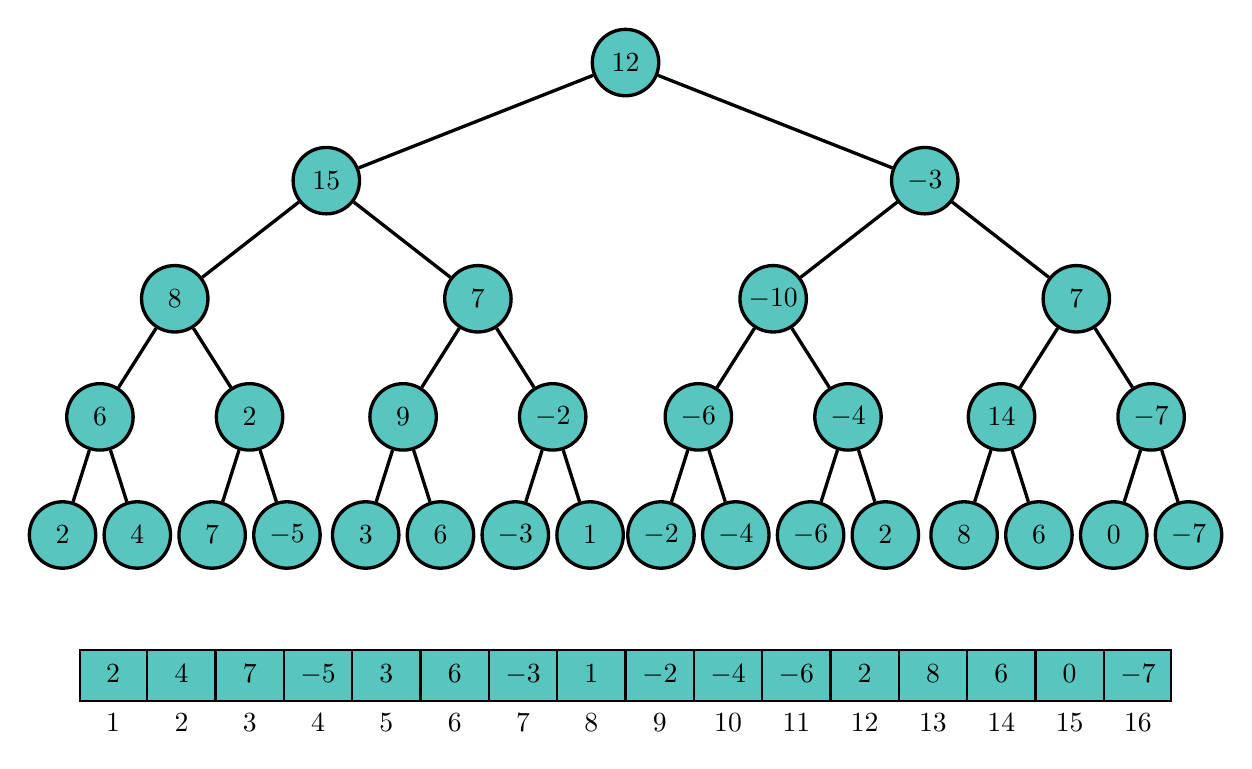
\begin{tikzpicture}[
  very thick,
  level 1/.style={sibling distance=76mm},
  level 2/.style={sibling distance=38.5mm},
  level 3/.style={sibling distance=19mm},
  level 4/.style={sibling distance=9.5mm},
  myrect/.style={
    draw,
    thick,
    fill=myseagreen,
    rectangle split,
    rectangle split horizontal,
    rectangle split parts=#1,
    rectangle split part align=left,
    text width=4ex,
    text centered
    }
]
\node [vertex] (r){$12$}
  child {
    node [vertex] (a) {15}
    child {
      node [vertex] {8}
      child {
        node [vertex] {6}
        child {node [vertex] {2}}
        child {node [vertex] {4}}
      } 
      child {
        node [vertex] {2}
        child {node [vertex] {7}}
        child {node [vertex] {$-5$}}
      }
    }
    child {
      node [vertex] {7}
      child {node [vertex] {9}
              child {node [vertex] {3}}
        child {node [vertex] {6}}
      }
      child {node [vertex] {$-2$}
              child {node [vertex] {$-3$}}
        child {node [vertex] {1}}
      }
    }
  }
  child {
    node [vertex] {$-3$}
    child {
      node [vertex] {$-10$}
      child {node [vertex] {$-6$}
              child {node [vertex] {$-2$}}
        child {node [vertex] {$-4$}}}
      child {node [vertex] {$-4$}
              child {node [vertex] {$-6$}}
        child {node [vertex] {$2$}}}
    }
    child {
      node [vertex] {7}
      child {node [vertex] {14}
              child {node [vertex] {8}}
        child {node [vertex] {6}}}
      child {node [vertex] {$-7$}
              child {node [vertex] {0}}
        child {node [vertex] {$-7$}}}
    }
  };

\node[myrect=16] [below=7cm of r]
  (array)
  {
  					\strut 2
  \nodepart{two}	\strut 4
  \nodepart{three}	\strut 7
  \nodepart{four}	\strut $-5$
  \nodepart{five}	\strut 3
  \nodepart{six}	\strut 6
  \nodepart{seven}	\strut $-3$
  \nodepart{eight}	\strut 1
  \nodepart{nine}	\strut $-2$
  \nodepart{ten}	\strut $-4$
  \nodepart{eleven}	\strut $-6$
  \nodepart{twelve}	\strut 2
  \nodepart{thirteen}	\strut 8
  \nodepart{fourteen}	\strut 6
  \nodepart{fifteen}	\strut 0
  \nodepart{sixteen}	\strut $-7$
  };
\foreach \Valor [count=\Valori from 1] in {one ,two ,three , four , five , six , seven , eight , nine , ten , eleven , twelve , thirteen , fourteen , fifteen , sixteen }
  \node[below] at (array.\Valor south) {\Valori};

\end{tikzpicture}
}
\end{center}

Highlighted are the nodes we'll need to access for $query(7,15)$. Notice how the subtrees associated with each of these nodes neatly covers the entire range $[7,15]$.

\begin{center}
{
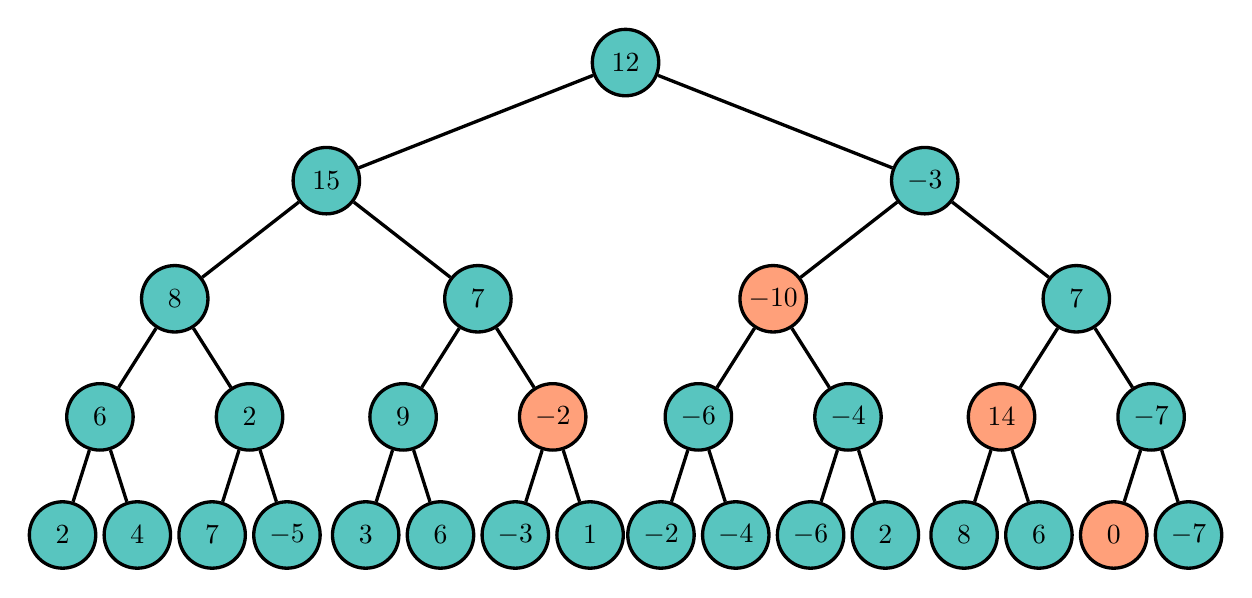
\begin{tikzpicture}[
  very thick,
  level 1/.style={sibling distance=76mm},
  level 2/.style={sibling distance=38.5mm},
  level 3/.style={sibling distance=19mm},
  level 4/.style={sibling distance=9.5mm},
  myrect/.style={
    draw,
    thick,
    fill=myseagreen,
    rectangle split,
    rectangle split horizontal,
    rectangle split parts=#1,
    rectangle split part align=left,
    text width=4ex,
    text centered
    }
]
\node [vertex] (r){$12$}
  child {
    node [vertex] (a) {15}
    child {
      node [vertex] {8}
      child {
        node [vertex] {6}
        child {node [vertex] {2}}
        child {node [vertex] {4}}
      } 
      child {
        node [vertex] {2}
        child {node [vertex] {7}}
        child {node [vertex] {$-5$}}
      }
    }
    child {
      node [vertex] {7}
      child {node [vertex] {9}
              child {node [vertex] {3}}
        child {node [vertex] {6}}
      }
      child {node [vertex, fill=mysalmon] {$-2$}
              child {node [vertex] {$-3$}}
        child {node [vertex] {1}}
      }
    }
  }
  child {
    node [vertex] {$-3$}
    child {
      node [vertex, fill=mysalmon] {$-10$}
      child {node [vertex] {$-6$}
              child {node [vertex] {$-2$}}
        child {node [vertex] {$-4$}}}
      child {node [vertex] {$-4$}
              child {node [vertex] {$-6$}}
        child {node [vertex] {$2$}}}
    }
    child {
      node [vertex] {7}
      child {node [vertex, fill=mysalmon] {14}
              child {node [vertex] {8}}
        child {node [vertex] {6}}}
      child {node [vertex] {$-7$}
              child {node [vertex, fill=mysalmon] {0}}
        child {node [vertex] {$-7$}}}
    }
  };

\end{tikzpicture}
}
\end{center}

$-2$ represents the sum $x_7+x_8$, $-10$ the sum $x_9+x_{10}+x_{11}+x_{12}$, $14$ the sum $x_{13}+x_{14}$, and $0$ represents the single element $x_{15}$. It seems we always want to take the \textit{largest} segments that stay within the range $[7,15]$. But how do we know exactly which segments these are?

We handle queries using a recursive call, starting at the root of the tree. We then proceed as follows: If the current node's interval is completely disjoint from the queried interval, we return 0. If the current node's interval is completely contained within the queried interval, we return the sum associated with that node. Otherwise, we pass the query on to the node's two children. Note that this process is $O(\log{n})$ because each level in the tree can have at most two highlighted nodes.

\noindent \begin{minipage}{\textwidth}
\begin{algorithmic}
\Function{Query}{range $[l,r]$, range $[a,b]$}
	\Comment at node $[l,r]$, want $\sum_{i=a}^b x_i$
	\If{$r < a$ or $b < l$}
		\Comment $[l,r] \cap [a,b] = \emptyset$
		\State \Return 0
	\EndIf
	\If{$a \le l$ and $r \le b$}
		\Comment $[l,r] \subseteq [a,b]$
		\State \Return $sum(l,r)$
	\EndIf
	\State \Return $\Call{Query}{\left[l,\floor{\frac{l+r}{2}}\right], [a,b]} + \Call{Query}{\left[\floor{\frac{l+r}{2}}+1,r \right], [a,b]}$
\EndFunction
\end{algorithmic}
\end{minipage}

Segment trees also handle modifications well. If we want to change the third element to 2, then we have to update the highlighted nodes in the following diagram. We can implement this the same way we implement queries. Starting from the root, we update each modified node's children before recomputing the value stored at that node. The complexity is $O(\log{n})$; we change the value of one node in each level of the tree.

\begin{center}
{
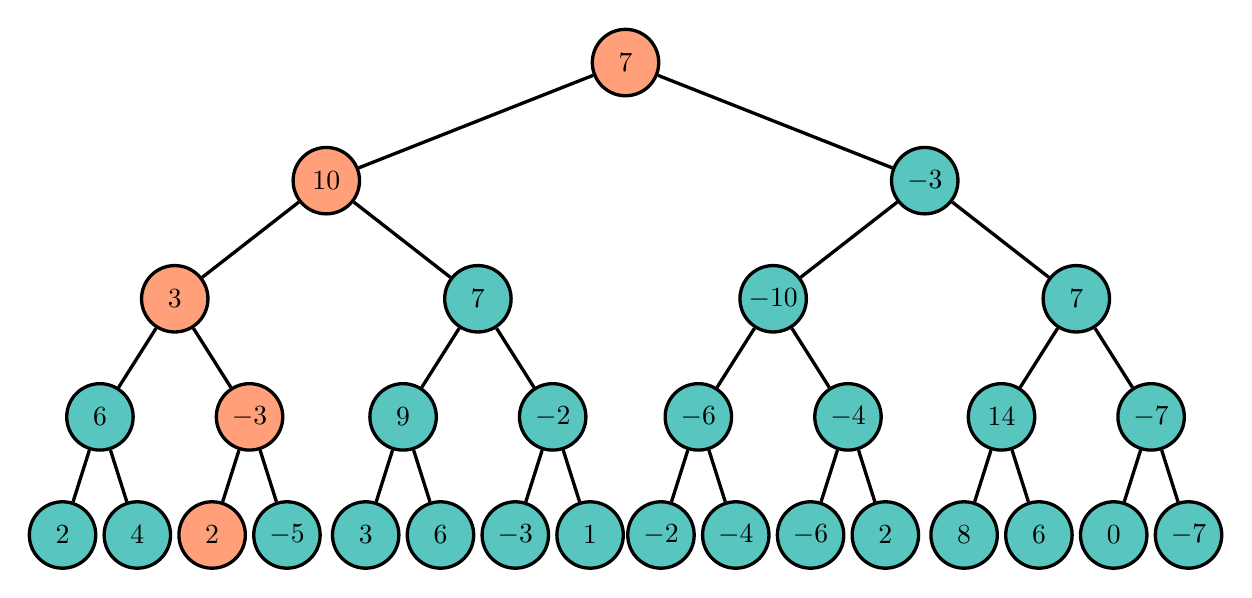
\begin{tikzpicture}[
  very thick,
  level 1/.style={sibling distance=76mm},
  level 2/.style={sibling distance=38.5mm},
  level 3/.style={sibling distance=19mm},
  level 4/.style={sibling distance=9.5mm},
  myrect/.style={
    draw,
    thick,
    fill=myseagreen,
    rectangle split,
    rectangle split horizontal,
    rectangle split parts=#1,
    rectangle split part align=left,
    text width=4ex,
    text centered
    }
]
\node [vertex, fill=mysalmon] (r){7}
  child {
    node [vertex, fill=mysalmon] (a) {10}
    child {
      node [vertex, fill=mysalmon] {3}
      child {
        node [vertex] {6}
        child {node [vertex] {2}}
        child {node [vertex] {4}}
      } 
      child {
        node [vertex, fill=mysalmon] {$-3$}
        child {node [vertex, fill=mysalmon] {2}}
        child {node [vertex] {$-5$}}
      }
    }
    child {
      node [vertex] {7}
      child {node [vertex] {9}
              child {node [vertex] {3}}
        child {node [vertex] {6}}
      }
      child {node [vertex] {$-2$}
              child {node [vertex] {$-3$}}
        child {node [vertex] {1}}
      }
    }
  }
  child {
    node [vertex] {$-3$}
    child {
      node [vertex] {$-10$}
      child {node [vertex] {$-6$}
              child {node [vertex] {$-2$}}
        child {node [vertex] {$-4$}}}
      child {node [vertex] {$-4$}
              child {node [vertex] {$-6$}}
        child {node [vertex] {$2$}}}
    }
    child {
      node [vertex] {7}
      child {node [vertex] {14}
              child {node [vertex] {8}}
        child {node [vertex] {6}}}
      child {node [vertex] {$-7$}
              child {node [vertex] {0}}
        child {node [vertex] {$-7$}}}
    }
  };

\end{tikzpicture}
}
\end{center}

\noindent \begin{minipage}{\textwidth}
\begin{algorithmic}
\Function{Update}{range $[l,r]$, $p$, $k$}
	\Comment $x_p \gets x_p + k$
	\If{$r < p$ or $p < l$}
		\Comment $p \not\in [l,r]$
		\State \Return
	\EndIf
	\If{$l = r$}
		\Comment leaf node
		\State $sum(l,r) \gets k$
		\State \Return
	\EndIf
	\State \Call{Update}{$\left[l,\floor{\frac{l+r}{2}}\right]$, $p$, $k$}
	\State \Call{Update}{$\left[\floor{\frac{l+r}{2}}+1,r\right]$, $p$, $k$}
	\State $sum(l,r) \gets sum(l,\floor{\frac{l+r}{2}}) + sum(\floor{\frac{l+r}{2}}+1,r)$
\EndFunction
\end{algorithmic}
\end{minipage}

I cheated with my example by using a nice power of two, $n=16$, as the number of elements in the sequence. Of course, the size is not always this nice. However, if we want a tree of size $n$, we can always round up to the nearest power of 2, which is at most $2n$. A perfectly balanced segment tree of size $n$ equalling a power of 2 requires $2n-1$ nodes representing our segments, so $4n$ bounds the memory we'll need.

Now all we need is a way for us to easily store the sum values associated with each node. We can clearly use a structure with two child pointers, but we can also exploit the fact that the segment tree structure is a balanced binary search tree. We can store the tree like we store a heap. The root is labeled 1, and for each node with label $i$, the left child is labeled $2i$ and the right child $2i + 1$. Here's some sample code.

\begin{mylstlisting}
final int SZ = 1 << 17; // some sufficiently large power of 2
int[] sum = new int[2 * SZ]; // sum[1] contains sum for [1, SZ], and so on
int query(int i, int l, int r, int a, int b) {
	// i.e. query(1, 1, SZ, 7, 15)
	if(r < a || b < l) return 0;
	if(a <= l && r <= b) return tree[i];
	int m = (l + r) / 2;
	int ql = query(2 * i, l, m, a, b);
	int qr = query(2 * i + 1, m + 1, r, a, b);
	return ql + qr;
}
void update(int i, int l, int r, int p, int k) {
	// i.e. update(1, 1, SZ, 3, 2)
	if(r < p || p < l) return;
	if(l == r){
		sum[i] = k;
		return;
	}
	int m = (l + r) / 2;
	update(2 * i, l, m, p, k);
	update(2 * i + 1, m + 1, r, p, k);
	sum[i] = sum[2 * i] + sum[2 * i + 1];
}
\end{mylstlisting}

Mathematically, what allows the segment tree to work on the addition operation lies in the fact that addition is an associative operation. This means that we can support a wide variety of other kinds of range queries, so long as the operation is associative. For example, we can also support range minimum queries and $gcd$ and $lcm$ queries. We can even combine different types of information stored at a node. One situation that requires this is maintaining the maximum prefix sum.

For our simple range sum query problem, we don't need the nice, completely balanced structure present when the number of elements is a nice power of two. However, it is necessary if we want to force the array $sum[]$ to have the same nice properties as an actual heap so we can perform nice iterative operations on our tree, as previously, all tree operations were recursive. It is also necessary if we need the numbers representing the indices in our tree to have special properties, as in the Fenwick tree.

\subsection{Lazy Propagation}

It is often the case that in addition to performing range queries, we need to perform \textit{range updates}. (Before, we only had to implement point updates.) One extension of our sum problem would require the following two functions:

\begin{itemize}
\item
$update(a, b, k)$ -- increment the value of $x_i$ by $k$ for all $i\in [a,b]$

\item
$query(a, b)$ -- return $\sum_{i=a}^b x_i$.
\end{itemize}

\subsubsection{Some Motivation: $\sqrt{n}$ Blocking}

Let's go back to our $\sqrt{n}$ blocking solution and see what changes we can make, and hopefully we can extend this idea back to our segment tree. If we're looking for an $O(\sqrt{n})$ implementation for $update$, we clearly can't perform point updates for all values in the range. The way we sped up $query$ was by keeping track of an extra set of data, the sum of all the elements in a bucket, which we used when \textit{the entire bucket was in the query range}.

\begin{center}
{
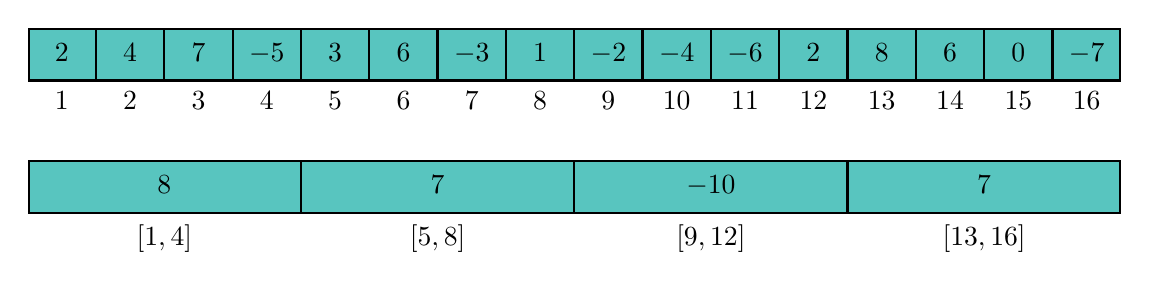
\begin{tikzpicture}[
  thick,
  myrect/.style={
    draw,
    fill=myseagreen,
    rectangle split,
    rectangle split horizontal,
    rectangle split parts=#1,
    rectangle split part align=left,
    text width=4ex,
    text centered
    }
]

\node[myrect=16]
  (array2)
  {
  					\strut 2
  \nodepart{two}	\strut 4
  \nodepart{three}	\strut 7
  \nodepart{four}	\strut $-5$
  \nodepart{five}	\strut 3
  \nodepart{six}	\strut 6
  \nodepart{seven}	\strut $-3$
  \nodepart{eight}	\strut 1
  \nodepart{nine}	\strut $-2$
  \nodepart{ten}	\strut $-4$
  \nodepart{eleven}	\strut $-6$
  \nodepart{twelve}	\strut 2
  \nodepart{thirteen}	\strut 8
  \nodepart{fourteen}	\strut 6
  \nodepart{fifteen}	\strut 0
  \nodepart{sixteen}	\strut $-7$
  };
\foreach \Valor [count=\Valori from 1] in {one ,two ,three , four , five , six , seven , eight , nine , ten , eleven , twelve , thirteen , fourteen , fifteen , sixteen }
  \node[below] at (array2.\Valor south) {\Valori};

\node[myrect=4, text width=21.2ex] [below=of array2]
  (array)
  {
  					\strut 8
  \nodepart{two}	\strut 7
  \nodepart{three}	\strut $-10$
  \nodepart{four}	\strut 7
  };

\node[below] at (array.one south) {$[1,4]$};
\node[below] at (array.two south) {$[5,8]$};
\node[below] at (array.three south) {$[9,12]$};
\node[below] at (array.four south) {$[13,16]$};
\end{tikzpicture}
}
\end{center}

Can we do something similar for $update$? The case we need to wory about is when an entire bucket is included in the update range. Again, we don't want to touch the original array $a$ at all, since that makes the operation linear. Instead, whenever we update an entire bucket, we track the information about the update separately. Thus we store a value for each bucket indicating the amount by which we've incremented that entire bucket.

With this in mind, highlighted are the elements we'll need for $update(4,14,3)$.

\begin{center}
{
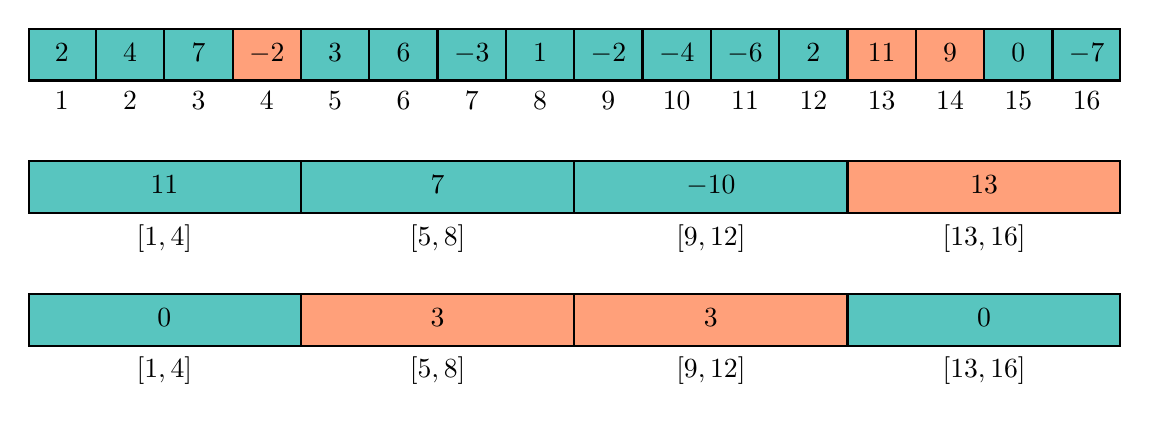
\begin{tikzpicture}[
  thick,
  myrect/.style={
    draw,
    rectangle split,
    rectangle split horizontal,
    rectangle split parts=#1,
    rectangle split part align=left,
    text width=4ex,
    text centered
    }
]

\node[myrect=16, rectangle split part fill={myseagreen, myseagreen, myseagreen, mysalmon, myseagreen, myseagreen, myseagreen, myseagreen, myseagreen, myseagreen, myseagreen, myseagreen, mysalmon, mysalmon, myseagreen, myseagreen}]
  (array2)
  {
  					\strut 2
  \nodepart{two}	\strut 4
  \nodepart{three}	\strut 7
  \nodepart{four}	\strut $-2$
  \nodepart{five}	\strut 3
  \nodepart{six}	\strut 6
  \nodepart{seven}	\strut $-3$
  \nodepart{eight}	\strut 1
  \nodepart{nine}	\strut $-2$
  \nodepart{ten}	\strut $-4$
  \nodepart{eleven}	\strut $-6$
  \nodepart{twelve}	\strut 2
  \nodepart{thirteen}	\strut 11
  \nodepart{fourteen}	\strut 9
  \nodepart{fifteen}	\strut 0
  \nodepart{sixteen}	\strut $-7$
  };
\foreach \Valor [count=\Valori from 1] in {one ,two ,three , four , five , six , seven , eight , nine , ten , eleven , twelve , thirteen , fourteen , fifteen , sixteen }
  \node[below] at (array2.\Valor south) {\Valori};

\node[myrect=4, text width=21.2ex, rectangle split part fill={myseagreen, myseagreen, myseagreen, mysalmon}] [below=of array2]
  (array)
  {
  					\strut 11
  \nodepart{two}	\strut 7
  \nodepart{three}	\strut $-10$
  \nodepart{four}	\strut 13
  };

\node[below] at (array.one south) {$[1,4]$};
\node[below] at (array.two south) {$[5,8]$};
\node[below] at (array.three south) {$[9,12]$};
\node[below] at (array.four south) {$[13,16]$};

\node[myrect=4, text width=21.2ex, rectangle split part fill={myseagreen, mysalmon, mysalmon, myseagreen}] [below=of array]
  (array3)
  {
  					\strut 0
  \nodepart{two}	\strut 3
  \nodepart{three}	\strut 3
  \nodepart{four}	\strut 0
  };

\node[below] at (array3.one south) {$[1,4]$};
\node[below] at (array3.two south) {$[5,8]$};
\node[below] at (array3.three south) {$[9,12]$};
\node[below] at (array3.four south) {$[13,16]$};
\end{tikzpicture}
}
\end{center}

To reiterate, we are not storing the actual values of the elements or buckets in the arrays, where they were stored when we solved the original formulation of the problem. Despite this fact, we can still calculate the value of any element or bucket. $a_i$ is equal to the sum of the $\ceiling{\frac{i}{\sqrt{n}}}$th value stored in the third array and the $i$th value stored in the first array. The sum of any given bucket can be calculated similarly. However, we must remember to adjust for bucket size. In the example, there are four elements per bucket, so we have to add $4 \cdot 3 = 12$ to get the correct sum for an updated bucket. Because of all this, we can query a range exactly like we did without range updates.

Highlighted are the values necessary for $query(7,15)$.

\begin{center}
{
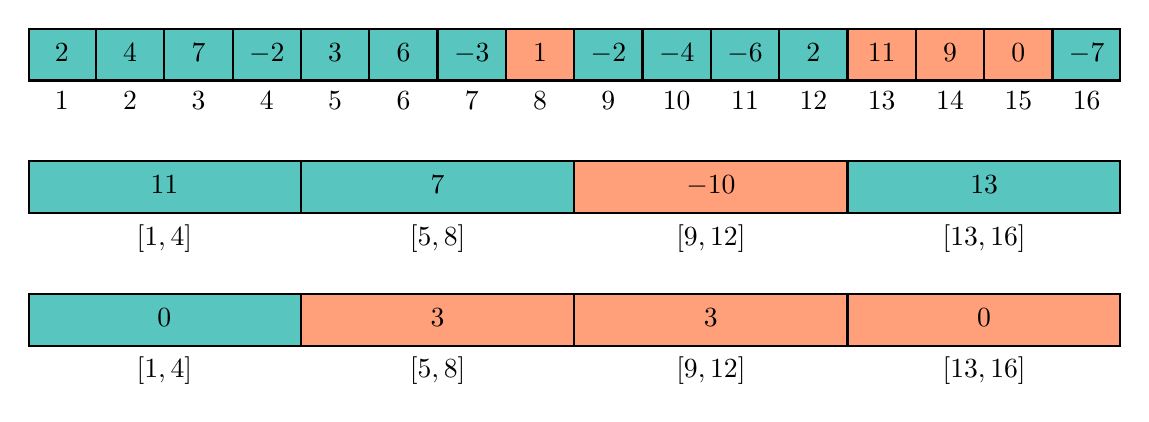
\begin{tikzpicture}[
  thick,
  myrect/.style={
    draw,
    rectangle split,
    rectangle split horizontal,
    rectangle split parts=#1,
    rectangle split part align=left,
    text width=4ex,
    text centered
    }
]

\node[myrect=16, rectangle split part fill={myseagreen, myseagreen, myseagreen, myseagreen, myseagreen, myseagreen, myseagreen, mysalmon, myseagreen, myseagreen, myseagreen, myseagreen, mysalmon, mysalmon, mysalmon, myseagreen}]
  (array2)
  {
  					\strut 2
  \nodepart{two}	\strut 4
  \nodepart{three}	\strut 7
  \nodepart{four}	\strut $-2$
  \nodepart{five}	\strut 3
  \nodepart{six}	\strut 6
  \nodepart{seven}	\strut $-3$
  \nodepart{eight}	\strut 1
  \nodepart{nine}	\strut $-2$
  \nodepart{ten}	\strut $-4$
  \nodepart{eleven}	\strut $-6$
  \nodepart{twelve}	\strut 2
  \nodepart{thirteen}	\strut 11
  \nodepart{fourteen}	\strut 9
  \nodepart{fifteen}	\strut 0
  \nodepart{sixteen}	\strut $-7$
  };
\foreach \Valor [count=\Valori from 1] in {one ,two ,three , four , five , six , seven , eight , nine , ten , eleven , twelve , thirteen , fourteen , fifteen , sixteen }
  \node[below] at (array2.\Valor south) {\Valori};

\node[myrect=4, text width=21.2ex, rectangle split part fill={myseagreen, myseagreen, mysalmon, myseagreen}] [below=of array2]
  (array)
  {
  					\strut 11
  \nodepart{two}	\strut 7
  \nodepart{three}	\strut $-10$
  \nodepart{four}	\strut 13
  };

\node[below] at (array.one south) {$[1,4]$};
\node[below] at (array.two south) {$[5,8]$};
\node[below] at (array.three south) {$[9,12]$};
\node[below] at (array.four south) {$[13,16]$};

\node[myrect=4, text width=21.2ex, rectangle split part fill={myseagreen, mysalmon, mysalmon, mysalmon}] [below=of array]
  (array3)
  {
  					\strut 0
  \nodepart{two}	\strut 3
  \nodepart{three}	\strut 3
  \nodepart{four}	\strut 0
  };

\node[below] at (array3.one south) {$[1,4]$};
\node[below] at (array3.two south) {$[5,8]$};
\node[below] at (array3.three south) {$[9,12]$};
\node[below] at (array3.four south) {$[13,16]$};
\end{tikzpicture}
}
\end{center}

Thus we have achieved an $O(\sqrt{n})$ solution for both range updates and and range queries.

\subsubsection{Lazy Propagation on a Segment Tree}

Motivated by how we fixed our bucketing solution, let's try adding a similar extra piece of information to our segment tree to try to get an $O(\log{n})$ solution. Call this extra value the ``lazy'' value.

\begin{center}
{
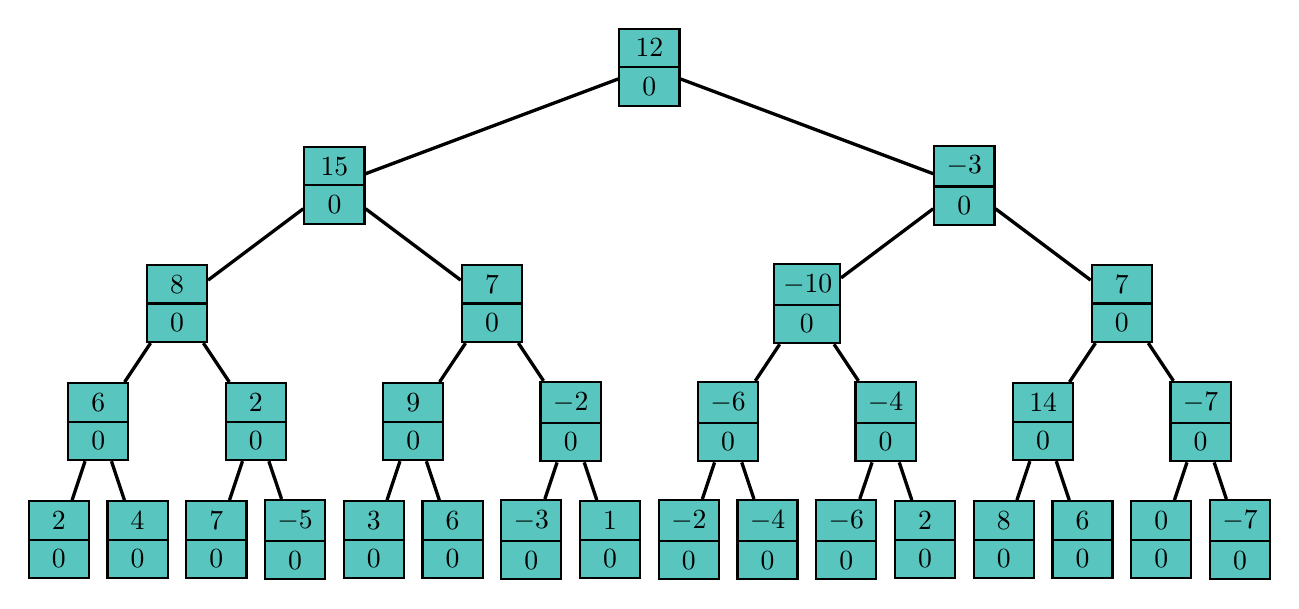
\begin{tikzpicture}[
  very thick,
  level 1/.style={sibling distance=80mm},
  level 2/.style={sibling distance=40mm},
  level 3/.style={sibling distance=20mm},
  level 4/.style={sibling distance=10mm},
  myrect/.style={
    draw,
    thick,
    fill=myseagreen,
    rectangle split,
    rectangle split parts=2,
    rectangle split part align=left,
    text width=3.5ex,
    text centered
    }
]
\node [myrect] (r){$12$\nodepart{two}0}
  child {
    node [myrect] (a) {15\nodepart{two}0}
    child {
      node [myrect] {8\nodepart{two}0}
      child {
        node [myrect] {6\nodepart{two}0}
        child {node [myrect] {2\nodepart{two}0}}
        child {node [myrect] {4\nodepart{two}0}}
      } 
      child {
        node [myrect] {2\nodepart{two}0}
        child {node [myrect] {7\nodepart{two}0}}
        child {node [myrect] {$-5$\nodepart{two}0}}
      }
    }
    child {
      node [myrect] {7\nodepart{two}0}
      child {node [myrect] {9\nodepart{two}0}
              child {node [myrect] {3\nodepart{two}0}}
        child {node [myrect] {6\nodepart{two}0}}
      }
      child {node [myrect] {$-2$\nodepart{two}0}
              child {node [myrect] {$-3$\nodepart{two}0}}
        child {node [myrect] {1\nodepart{two}0}}
      }
    }
  }
  child {
    node [myrect] {$-3$\nodepart{two}0}
    child {
      node [myrect, text width=4ex] {$-10$\nodepart{two}0}
      child {node [myrect] {$-6$\nodepart{two}0}
              child {node [myrect] {$-2$\nodepart{two}0}}
        child {node [myrect] {$-4$\nodepart{two}0}}}
      child {node [myrect] {$-4$\nodepart{two}0}
              child {node [myrect] {$-6$\nodepart{two}0}}
        child {node [myrect] {$2$\nodepart{two}0}}}
    }
    child {
      node [myrect] {7\nodepart{two}0}
      child {node [myrect] {14\nodepart{two}0}
              child {node [myrect] {8\nodepart{two}0}}
        child {node [myrect] {6\nodepart{two}0}}}
      child {node [myrect] {$-7$\nodepart{two}0}
              child {node [myrect] {0\nodepart{two}0}}
        child {node [myrect] {$-7$\nodepart{two}0}}}
    }
  };

\end{tikzpicture}
}
\end{center}

Once again, if the entire range associated with a node is contained within the update interval, we'll just make a note of it on that particular node and not update that node or any of its children. We'll call such a node ``lazy.''

Here's the status of the tree after $update(3,12,2)$.

\begin{center}
{
\begin{tikzpicture}[
  very thick,
  level 1/.style={sibling distance=80mm},
  level 2/.style={sibling distance=40mm},
  level 3/.style={sibling distance=20mm},
  level 4/.style={sibling distance=10mm},
  myrect/.style={
    draw,
    thick,
    rectangle split,
    rectangle split parts=2,
    rectangle split part fill={myseagreen, myseagreen},
    rectangle split part align=left,
    text width=3.5ex,
    text centered
    }
]
\node [myrect, rectangle split part fill={mysalmon, myseagreen}] (r){$32$\nodepart{two}0}
  child {
    node [myrect, rectangle split part fill={mysalmon, myseagreen}] (a) {27\nodepart{two}0}
    child {
      node [myrect, rectangle split part fill={mysalmon, myseagreen}] {12\nodepart{two}0}
      child {
        node [myrect] {6\nodepart{two}0}
        child {node [myrect] {2\nodepart{two}0}}
        child {node [myrect] {4\nodepart{two}0}}
      } 
      child {
        node [myrect, rectangle split part fill={myseagreen, mysalmon}] {2\nodepart{two}2}
        child {node [myrect] {7\nodepart{two}0}}
        child {node [myrect] {$-5$\nodepart{two}0}}
      }
    }
    child {
      node [myrect, rectangle split part fill={myseagreen, mysalmon}] {7\nodepart{two}2}
      child {node [myrect] {9\nodepart{two}0}
              child {node [myrect] {3\nodepart{two}0}}
        child {node [myrect] {6\nodepart{two}0}}
      }
      child {node [myrect] {$-2$\nodepart{two}0}
              child {node [myrect] {$-3$\nodepart{two}0}}
        child {node [myrect] {1\nodepart{two}0}}
      }
    }
  }
  child {
    node [myrect, rectangle split part fill={mysalmon, myseagreen}] {$5$\nodepart{two}0}
    child {
      node [myrect, text width=4ex, rectangle split part fill={myseagreen, mysalmon}] {$-10$\nodepart{two}2}
      child {node [myrect] {$-6$\nodepart{two}0}
              child {node [myrect] {$-2$\nodepart{two}0}}
        child {node [myrect] {$-4$\nodepart{two}0}}}
      child {node [myrect] {$-4$\nodepart{two}0}
              child {node [myrect] {$-6$\nodepart{two}0}}
        child {node [myrect] {$2$\nodepart{two}0}}}
    }
    child {
      node [myrect] {7\nodepart{two}0}
      child {node [myrect] {14\nodepart{two}0}
              child {node [myrect] {8\nodepart{two}0}}
        child {node [myrect] {6\nodepart{two}0}}}
      child {node [myrect] {$-7$\nodepart{two}0}
              child {node [myrect] {0\nodepart{two}0}}
        child {node [myrect] {$-7$\nodepart{two}0}}}
    }
  };

\end{tikzpicture}
}
\end{center}

When a node is lazy, it indicates that the sum numbers of every node in its subtree are no longer accurate. In particular, if a node is lazy, the sum number it holds is not equal to the sum of the values in its leaves. This means that whenever we need to access any node in the subtree of that node, we'll need to update some values.

Suppose we encounter a lazy node while traversing down the tree. In order to get accurate sum values in that node's subtree, we need to apply the changes indicated by its lazy value. Thus we update the node's sum value, incrementing by the lazy value once for each leaf in the node's subtree. In addition, we have to propagate the lazy value to the node's children. We do this by incrementing each child's lazy value by our current node's lazy value. And finally, we need to set the lazy value to $0$, to indicate that there's nothing left to update. When we implement a segment tree, all of this is usually encapsulated within a ``push'' function.

Let's illustrate querying with an example: $query(7,13)$. To answer this, we need to access the nodes for the ranges $[7,8]$, $[9,12]$, and $[13,13]$. The node for $[13,13]$ is up-to-date and stores the correct sum. However, the other two nodes do not. (The node for $[7,8]$ is in the subtree of the node for $[5,8]$, which is lazy.) Thus as we recurse, we push our lazy values whenever we encounter them. Highlighted are the nodes we'll need to update for the query. Notice how $[5,8]$ and $[9,12]$ simply pass their lazy numbers to their children, where they'll update themselves when necessary.

\begin{center}
{
\begin{tikzpicture}[
  very thick,
  level 1/.style={sibling distance=80mm},
  level 2/.style={sibling distance=40mm},
  level 3/.style={sibling distance=20mm},
  level 4/.style={sibling distance=10mm},
  myrect/.style={
    draw,
    thick,
    rectangle split,
    rectangle split parts=2,
    rectangle split part fill={myseagreen, myseagreen},
    rectangle split part align=left,
    text width=3.5ex,
    text centered
    }
]
\node [myrect] (r){$32$\nodepart{two}0}
  child {
    node [myrect] (a) {27\nodepart{two}0}
    child {
      node [myrect] {12\nodepart{two}0}
      child {
        node [myrect] {6\nodepart{two}0}
        child {node [myrect] {2\nodepart{two}0}}
        child {node [myrect] {4\nodepart{two}0}}
      } 
      child {
        node [myrect] {2\nodepart{two}2}
        child {node [myrect] {7\nodepart{two}0}}
        child {node [myrect] {$-5$\nodepart{two}0}}
      }
    }
    child {
      node [myrect, rectangle split part fill={mysalmon, mysalmon}] {15\nodepart{two}0}
      child {
        node [myrect, rectangle split part fill={myseagreen, mysalmon}] {9\nodepart{two}2}
        child {node [myrect] {3\nodepart{two}0}}
        child {node [myrect] {6\nodepart{two}0}}
      }
      child {
        node [myrect, rectangle split part fill={mysalmon, mysalmon}] {$2$\nodepart{two}0}
        child {node [myrect, rectangle split part fill={myseagreen, mysalmon}] {$-3$\nodepart{two}2}}
        child {node [myrect, rectangle split part fill={myseagreen, mysalmon}] {1\nodepart{two}2}}
      }
    }
  }
  child {
    node [myrect] {$5$\nodepart{two}0}
    child {
      node [myrect, rectangle split part fill={mysalmon, mysalmon}] {$-2$\nodepart{two}0}
      child {node [myrect, rectangle split part fill={myseagreen, mysalmon}] {$-6$\nodepart{two}2}
              child {node [myrect] {$-2$\nodepart{two}0}}
        child {node [myrect] {$-4$\nodepart{two}0}}}
      child {node [myrect, rectangle split part fill={myseagreen, mysalmon}] {$-4$\nodepart{two}2}
              child {node [myrect] {$-6$\nodepart{two}0}}
        child {node [myrect] {$2$\nodepart{two}0}}}
    }
    child {
      node [myrect] {7\nodepart{two}0}
      child {node [myrect] {14\nodepart{two}0}
              child {node [myrect] {8\nodepart{two}0}}
        child {node [myrect] {6\nodepart{two}0}}}
      child {node [myrect] {$-7$\nodepart{two}0}
              child {node [myrect] {0\nodepart{two}0}}
        child {node [myrect] {$-7$\nodepart{two}0}}}
    }
  };

\end{tikzpicture}
}
\end{center}

The complexity of querying remains the same, even when propagating lazy values. We have to push at most once for each node we encounter, so our runtime is multiplied only by a constant factor. Thus, like normal segment tree queries, lazy segment tree queries also run in $O(\log n)$.

While we're thinking about complexity, we can also ask ourselves why it \emph{doesn't} take $O(n)$ time to update $O(n)$ nodes. With lazy propagation, we take advantage of two things. The first is that on each query, we access very few nodes, so as long as the nodes we access are up-to-date, we're all set. The second is that we can combine updates while they're still being propagated, that the update operation is associative. This allows us to update only when it's absolutely necessary---the rest of the time, we can be lazy. (The next time someone tells you you're being lazy, you can say it's a good thing.)

Like normal segment trees, lazily propagating segment trees can handle a diverse set of range updates and range queries. We can support an update, where instead of \textit{incrementing} each element on a range \textit{by} a certain value, we \textit{set} each element \textit{to} that value. There is no difference between the two as point updates, but they are very different operations when applied as range updates. Sometimes, we can even have more than one range update on a single tree. When implementing this, however, it is important to be careful when pushing lazy values---composing different operations can become quite complicated.

Below is my implementation of a segment tree supporting range sum and range increment. Note that it includes one detail that we left out in our development of lazy propagation above: how we update a node whose range partially intersects the updated range. One way to do this is to calculate the length of the intersection and update directly. However, this does not work well for queries that are not as nice as incrementing, such as setting an entire range to a value. Instead, we first update the children of this node. Then we push the lazy values off the children so their sum values are accurate. This allows us to recalculate the sum value of the parent like we do for a non-lazy segtree. I have this as my \texttt{pull} function below.

\begin{mylstlisting}
final int SZ = 1 << 17;
int[] sum = new int[2 * SZ];
int[] lazy = new int[2 * SZ];

void push(int i, int l, int r){
  if(lazy[i] != 0){
    sum[i] += (r - l + 1) * lazy[i];
    if(l < r){
      lazy[2 * i] += lazy[i];
      lazy[2 * i + 1] += lazy[i];
    }
    lazy[i] = 0;
  }
}

void pull(int i, int l, int r){
  int m = (l + r) / 2;
  push(2 * i, l, m);
  push(2 * i + 1, m + 1, r);
  sum[i] = sum[2 * i] + sum[2 * i + 1];
}

int query(int i, int l, int r, int a, int b) {
  push(i, l, r);
  if(r < a || b < l) return 0;
  if(a <= l && r <= b){
    return sum[i];
  }
  int m = (l + r) / 2;
  int ql = query(2 * i, l, m, a, b);
  int qr = query(2 * i + 1, m + 1, r, a, b);
  return ql + qr;
}

void update(int i, int l, int r, int a, int b, int k) {
  // push(i, l, r); // Necessary for non-commutative range updates.
  if(r < a || b < l) return;
  if(a <= l && r <= b){
    lazy[i] += k;
    return;
  }
  int m = (l + r) / 2;
  update(2 * i, l, m, a, b, k);
  update(2 * i + 1, m + 1, r, a, b, k);
  pull(i, l, r);
}
\end{mylstlisting}

\subsection{Fenwick Tree}

A \textit{Fenwick tree}, or \textit{binary indexed tree (BIT)}, is simply a faster and easier to code segment tree when the operator in question, in addition to being associative, has an inverse. Unfortunately, it's not at all intuitive, so bear with me at first and let the magic of the Fenwick tree reveal itself later.\footnote{In fact, it is so magical that Richard Peng hates it because it is too gimmicky.} The key idea is to compress the data stored within a segment tree in a crazy way that ends up having a really slick implementation using some bit operation tricks.

As discussed earlier, the $+$ operator has an inverse, $-$. Therefore, there is an inherent redundancy, for example, in keeping track of the sum of the first $\frac{n}{2}$ elements, the sum of all $n$ elements, and the sum of the last $\frac{n}{2}$ elements, as we do in the segment tree. If we are given only $\sum_{k=1}^{n/2} a_k$ and $\sum_{k=1}^n a_k$, we can find $\sum_{k=n/2+1}^{n} a_k$ easily using subtraction.

With this in mind, let's ignore every right child in the tree. We'll mark them as black in the diagram. After that, we'll write out the tree nodes in postfix traversal order, without writing anything whenever we encounter a black node.

\begin{center}
{
\begin{tikzpicture}[
  very thick,
  level 1/.style={sibling distance=76mm},
  level 2/.style={sibling distance=38.5mm},
  level 3/.style={sibling distance=19mm},
  level 4/.style={sibling distance=9.5mm},
  myrect/.style={
    draw,
    thick,
    fill=myseagreen,
    rectangle split,
    rectangle split horizontal,
    rectangle split parts=#1,
    rectangle split part align=left,
    text width=4ex,
    text centered
    }
]
\node [vertex] (r){$12$}
  child {
    node [vertex] (a) {15}
    child {
      node [vertex] {8}
      child {
        node [vertex] {6}
        child {node [vertex] {2}}
        child {node [vertex, text=mywhite, fill=myblack] {4}}
      } 
      child {
        node [vertex, text=mywhite, fill=myblack] {2}
        child {node [vertex] {7}}
        child {node [vertex, text=mywhite, fill=myblack] {$-5$}}
      }
    }
    child {
      node [vertex, text=mywhite, fill=myblack] {7}
      child {node [vertex] {9}
              child {node [vertex] {3}}
        child {node [vertex, text=mywhite, fill=myblack] {6}}
      }
      child {node [vertex, text=mywhite, fill=myblack] {$-2$}
              child {node [vertex] {$-3$}}
        child {node [vertex, text=mywhite, fill=myblack] {1}}
      }
    }
  }
  child {
    node [vertex, text=mywhite, fill=myblack] {$-3$}
    child {
      node [vertex] {$-10$}
      child {node [vertex] {$-6$}
              child {node [vertex] {$-2$}}
        child {node [vertex, text=mywhite, fill=myblack] {$-4$}}}
      child {node [vertex, text=mywhite, fill=myblack] {$-4$}
              child {node [vertex] {$-6$}}
        child {node [vertex, text=mywhite, fill=myblack] {$2$}}}
    }
    child {
      node [vertex, text=mywhite, fill=myblack] {7}
      child {node [vertex] {14}
              child {node [vertex] {8}}
        child {node [vertex, text=mywhite, fill=myblack] {6}}}
      child {node [vertex, text=mywhite, fill=myblack] {$-7$}
              child {node [vertex] {0}}
        child {node [vertex, text=mywhite, fill=myblack] {$-7$}}}
    }
  };

\node[myrect=16] [below=7cm of r]
  (array)
  {
  					\strut 2
  \nodepart{two}	\strut 4
  \nodepart{three}	\strut 7
  \nodepart{four}	\strut $-5$
  \nodepart{five}	\strut 3
  \nodepart{six}	\strut 6
  \nodepart{seven}	\strut $-3$
  \nodepart{eight}	\strut 1
  \nodepart{nine}	\strut $-2$
  \nodepart{ten}	\strut $-4$
  \nodepart{eleven}	\strut $-6$
  \nodepart{twelve}	\strut 2
  \nodepart{thirteen}	\strut 8
  \nodepart{fourteen}	\strut 6
  \nodepart{fifteen}	\strut 0
  \nodepart{sixteen}	\strut $-7$
  };
\foreach \Valor [count=\Valori from 1] in {one ,two ,three , four , five , six , seven , eight , nine , ten , eleven , twelve , thirteen , fourteen , fifteen , sixteen }
  \node[below] at (array.\Valor south) {\Valori};

\node[myrect=16] [below=of array]
  (array2)
  {
  					\strut 2
  \nodepart{two}	\strut 6
  \nodepart{three}	\strut 7
  \nodepart{four}	\strut 8
  \nodepart{five}	\strut 3
  \nodepart{six}	\strut 9
  \nodepart{seven}	\strut $-3$
  \nodepart{eight}	\strut 15
  \nodepart{nine}	\strut $-2$
  \nodepart{ten}	\strut $-6$
  \nodepart{eleven}	\strut $-6$
  \nodepart{twelve}	\strut $-10$
  \nodepart{thirteen}	\strut 8
  \nodepart{fourteen}	\strut 14
  \nodepart{fifteen}	\strut 0
  \nodepart{sixteen}	\strut 12
  };
\foreach \Valor [count=\Valori from 1] in {one ,two ,three , four , five , six , seven , eight , nine , ten , eleven , twelve , thirteen , fourteen , fifteen , sixteen }
  \node[below] at (array2.\Valor south) {\Valori};

\end{tikzpicture}
}
\end{center}

Our Fenwick tree is simply this last array. This should be quite confusing -- it is not at all clear why this array resembles a tree, and the numbers in the array make no sense whatsoever right now.

Notice that the final position of every unblackened node is just the rightmost black child in its subtree. This leads to the fact that the $i$th element in the Fenwick tree array is the sum

\[y_i = \sum_{k=i-2^{v_2(i)}+1}^i x_k, \]

where $2^{v_2(i)}$ is simply the greatest power of 2 that divides $i$. Let's look at a new diagram that hopefully will better illustrate this key property of the random array we just came up with.

\begin{center}
{
\begin{tikzpicture}[
  very thick,
  myrect/.style={
    draw,
    thick,
    fill=myseagreen,
    rectangle split,
    rectangle split horizontal,
    rectangle split parts=#1,
    rectangle split part align=left,
    text width=4ex,
    text centered
    },
  onesided/.style={
        text width=4ex,
        draw=none,
        append after command={
            [shorten <= -0.5\pgflinewidth] 
            ([shift={( 0.5\pgflinewidth,-0.5\pgflinewidth)}]\tikzlastnode.north west)
        edge([shift={( 0.5\pgflinewidth,+0.5\pgflinewidth)}]\tikzlastnode.south west)            
        }
    }
]

\node[myrect=16]
  (array)
  {
  					\strut 2
  \nodepart{two}	\strut 4
  \nodepart{three}	\strut 7
  \nodepart{four}	\strut $-5$
  \nodepart{five}	\strut 3
  \nodepart{six}	\strut 6
  \nodepart{seven}	\strut $-3$
  \nodepart{eight}	\strut 1
  \nodepart{nine}	\strut $-2$
  \nodepart{ten}	\strut $-4$
  \nodepart{eleven}	\strut $-6$
  \nodepart{twelve}	\strut 2
  \nodepart{thirteen}	\strut 8
  \nodepart{fourteen}	\strut 6
  \nodepart{fifteen}	\strut 0
  \nodepart{sixteen}	\strut $-7$
  };
\foreach \Valor [count=\Valori from 1] in {one ,two ,three , four , five , six , seven , eight , nine , ten , eleven , twelve , thirteen , fourteen , fifteen , sixteen }
  \node[below] at (array.\Valor south) {\Valori};

\node[myrect=1, above=5mm] at (array.one north) (n1) {2};
\node[myrect=1, above=15mm] at (array.two north) (n2) {6};
\node[myrect=1, above=5mm] at (array.three north) (n3) {7};
\node[myrect=1, above=25mm] at (array.four north) (n4) {8};
\node[myrect=1, above=5mm] at (array.five north) (n5) {3};
\node[myrect=1, above=15mm] at (array.six north) (n6) {9};
\node[myrect=1, above=5mm] at (array.seven north) (n7) {$-3$};
\node[myrect=1, above=35mm] at (array.eight north) (n8) {15};
\node[myrect=1, above=5mm] at (array.nine north) (n9) {$-2$};
\node[myrect=1, above=15mm] at (array.ten north) (n10) {$-6$};
\node[myrect=1, above=5mm] at (array.eleven north) (n11) {$-6$};
\node[myrect=1, above=25mm] at (array.twelve north) (n12) {$-10$};
\node[myrect=1, above=5mm] at (array.thirteen north) (n13) {8};
\node[myrect=1, above=15mm] at (array.fourteen north) (n14) {14};
\node[myrect=1, above=5mm] at (array.fifteen north) (n15) {0};
\node[myrect=1, above=45mm] at (array.sixteen north) (n16) {12};

\node[onesided, above=15mm] at (array.one north) (m2) { \phantom{0} };
\node[onesided, above=25mm] at (array.one north) (m4) { \phantom{0} };
\node[onesided, above=15mm] at (array.five north) (m6) { \phantom{0} };
\node[onesided, above=35mm] at (array.one north) (m8) { \phantom{0} };
\node[onesided, above=15mm] at (array.nine north) (m10) { \phantom{0} };
\node[onesided, above=25mm] at (array.nine north) (m12) { \phantom{0} };
\node[onesided, above=15mm] at (array.thirteen north) (m14) { \phantom{0} };
\node[onesided, above=45mm] at (array.one north) (m16) { \phantom{0} };

\draw (m2.west) -- (n2.west);
\draw (m4.west) -- (n4.west);
\draw (m6.west) -- (n6.west);
\draw (m8.west) -- (n8.west);
\draw (m10.west) -- (n10.west);
\draw (m12.west) -- (n12.west);
\draw (m14.west) -- (n14.west);
\draw (m16.west) -- (n16.west);

\node[myrect=16] [below=of array]
  (array2)
  {
  					\strut 2
  \nodepart{two}	\strut 6
  \nodepart{three}	\strut 7
  \nodepart{four}	\strut 8
  \nodepart{five}	\strut 3
  \nodepart{six}	\strut 9
  \nodepart{seven}	\strut $-3$
  \nodepart{eight}	\strut 15
  \nodepart{nine}	\strut $-2$
  \nodepart{ten}	\strut $-6$
  \nodepart{eleven}	\strut $-6$
  \nodepart{twelve}	\strut $-10$
  \nodepart{thirteen}	\strut 8
  \nodepart{fourteen}	\strut 14
  \nodepart{fifteen}	\strut 0
  \nodepart{sixteen}	\strut 12
  };
\foreach \Valor [count=\Valori from 1] in {one ,two ,three , four , five , six , seven , eight , nine , ten , eleven , twelve , thirteen , fourteen , fifteen , sixteen }
  \node[below] at (array2.\Valor south) {\Valori};

\end{tikzpicture}
}
\end{center}

All the framework is now in place. Now we need to find out how to query and update the Fenwick tree.

Suppose we wanted to find the sum $\sum_{k=1}^{11} x_k$. Let's take a look at the diagram to see which elements we need.

\begin{center}
{
\begin{tikzpicture}[
  very thick,
  myrect2/.style={
    draw,
    thick,
    rectangle split,
    rectangle split horizontal,
    rectangle split parts=#1,
    rectangle split part align=left,
    text width=4ex,
    text centered
    },
  myrect/.style={
    draw,
    thick,
    rectangle split,
    rectangle split horizontal,
    rectangle split parts=#1,
    fill=myseagreen,
    rectangle split part align=left,
    text width=4ex,
    text centered,
  	fill=myseagreen
  },
  onesided/.style={
        text width=4ex,
        draw=none,
        append after command={
            [shorten <= -0.5\pgflinewidth] 
            ([shift={( 0.5\pgflinewidth,-0.5\pgflinewidth)}]\tikzlastnode.north west)
        edge([shift={( 0.5\pgflinewidth,+0.5\pgflinewidth)}]\tikzlastnode.south west)            
        }
    }
]

\node[myrect=16]
  (array)
  {
  					\strut 2
  \nodepart{two}	\strut 4
  \nodepart{three}	\strut 7
  \nodepart{four}	\strut $-5$
  \nodepart{five}	\strut 3
  \nodepart{six}	\strut 6
  \nodepart{seven}	\strut $-3$
  \nodepart{eight}	\strut 1
  \nodepart{nine}	\strut $-2$
  \nodepart{ten}	\strut $-4$
  \nodepart{eleven}	\strut $-6$
  \nodepart{twelve}	\strut 2
  \nodepart{thirteen}	\strut 8
  \nodepart{fourteen}	\strut 6
  \nodepart{fifteen}	\strut 0
  \nodepart{sixteen}	\strut $-7$
  };
\foreach \Valor [count=\Valori from 1] in {one ,two ,three , four , five , six , seven , eight , nine , ten , eleven , twelve , thirteen , fourteen , fifteen , sixteen }
  \node[below] at (array.\Valor south) {\Valori};

\node[myrect=1, above=5mm] at (array.one north) (n1) {2};
\node[myrect=1, above=15mm] at (array.two north) (n2) {6};
\node[myrect=1, above=5mm] at (array.three north) (n3) {7};
\node[myrect=1, above=25mm] at (array.four north) (n4) {8};
\node[myrect=1, above=5mm] at (array.five north) (n5) {3};
\node[myrect=1, above=15mm] at (array.six north) (n6) {9};
\node[myrect=1, above=5mm] at (array.seven north) (n7) {$-3$};
\node[myrect=1, above=35mm, fill=mysalmon] at (array.eight north) (n8) {15};
\node[myrect=1, above=5mm] at (array.nine north) (n9) {$-2$};
\node[myrect=1, above=15mm, fill=mysalmon] at (array.ten north) (n10) {$-6$};
\node[myrect=1, above=5mm, fill=mysalmon] at (array.eleven north) (n11) {$-6$};
\node[myrect=1, above=25mm] at (array.twelve north) (n12) {$-10$};
\node[myrect=1, above=5mm] at (array.thirteen north) (n13) {8};
\node[myrect=1, above=15mm] at (array.fourteen north) (n14) {14};
\node[myrect=1, above=5mm] at (array.fifteen north) (n15) {0};
\node[myrect=1, above=45mm] at (array.sixteen north) (n16) {12};

\node[onesided, above=15mm] at (array.one north) (m2) { \phantom{0} };
\node[onesided, above=25mm] at (array.one north) (m4) { \phantom{0} };
\node[onesided, above=15mm] at (array.five north) (m6) { \phantom{0} };
\node[onesided, above=35mm] at (array.one north) (m8) { \phantom{0} };
\node[onesided, above=15mm] at (array.nine north) (m10) { \phantom{0} };
\node[onesided, above=25mm] at (array.nine north) (m12) { \phantom{0} };
\node[onesided, above=15mm] at (array.thirteen north) (m14) { \phantom{0} };
\node[onesided, above=45mm] at (array.one north) (m16) { \phantom{0} };

\draw (m2.west) -- (n2.west);
\draw (m4.west) -- (n4.west);
\draw (m6.west) -- (n6.west);
\draw (m8.west) -- (n8.west);
\draw (m10.west) -- (n10.west);
\draw (m12.west) -- (n12.west);
\draw (m14.west) -- (n14.west);
\draw (m16.west) -- (n16.west);

\node[myrect2=16, rectangle split part fill={myseagreen, myseagreen, myseagreen, myseagreen, myseagreen, myseagreen, myseagreen, mysalmon, myseagreen, myseagreen, mysalmon, myseagreen, myseagreen, myseagreen, myseagreen, myseagreen}] [below=of array]
  (array2)
  {
  					\strut 2
  \nodepart{two}	\strut 6
  \nodepart{three}	\strut 7
  \nodepart{four}	\strut 8
  \nodepart{five}	\strut 3
  \nodepart{six}	\strut 9
  \nodepart{seven}	\strut $-3$
  \nodepart{eight}	\strut 15
  \nodepart{nine}	\strut $-2$
  \nodepart{ten}	\strut $-6$
  \nodepart{eleven}	\strut $-6$
  \nodepart{twelve}	\strut $-10$
  \nodepart{thirteen}	\strut 8
  \nodepart{fourteen}	\strut 14
  \nodepart{fifteen}	\strut 0
  \nodepart{sixteen}	\strut 12
  };
\foreach \Valor [count=\Valori from 1] in {one ,two ,three , four , five , six , seven , eight , nine , ten , eleven , twelve , thirteen , fourteen , fifteen , sixteen }
  \node[below] at (array2.\Valor south) {\Valori};

\end{tikzpicture}
}
\end{center}

We see that the sum $\sum_{k=1}^{11}x_k=y_8+y_{10}+y_{11}$. If we look at 11 in binary, we have $11=01011_2$. Let's see if we can find a pattern in these numbers in binary:

\begin{align*}
11 &= 01011_2, \\
10 = 11-2^{v_2(11)} &= 01010_2, \\
8 = 10-2^{v_2(10)} &= 01000_2, \\
0=8-2^{v_2(8)}&=00000_2.
\end{align*}

So, we can simply subtract $11-2^{v_2(11)}=10=01010_2$, find the sum of the first 10 elements, and add $b_{11}$ to that sum to get the sum of the first 11 elements. We see that repeating this process takes off the last 1 in the binary representation of the number $i$, and since there are at most $\log{n}+1$ 1s in the binary representation $\forall i \in [1,n]$, the query operation is $O(\log{n})$.

And now for the update operation. Suppose we want to change the value of $x_{11}$ from $-6$ to $-3$. Which numbers will we have to change?

\begin{center}
{
\begin{tikzpicture}[
  very thick,
  myrect2/.style={
    draw,
    thick,
    rectangle split,
    rectangle split horizontal,
    rectangle split parts=#1,
    rectangle split part align=left,
    text width=4ex,
    text centered
    },
  myrect/.style={
    draw,
    thick,
    rectangle split,
    rectangle split horizontal,
    rectangle split parts=#1,
    fill=myseagreen,
    rectangle split part align=left,
    text width=4ex,
    text centered,
  	fill=myseagreen
  },
  onesided/.style={
        text width=4ex,
        draw=none,
        append after command={
            [shorten <= -0.5\pgflinewidth] 
            ([shift={( 0.5\pgflinewidth,-0.5\pgflinewidth)}]\tikzlastnode.north west)
        edge([shift={( 0.5\pgflinewidth,+0.5\pgflinewidth)}]\tikzlastnode.south west)            
        }
    }
]

\node[myrect=16]
  (array)
  {
  					\strut 2
  \nodepart{two}	\strut 4
  \nodepart{three}	\strut 7
  \nodepart{four}	\strut $-5$
  \nodepart{five}	\strut 3
  \nodepart{six}	\strut 6
  \nodepart{seven}	\strut $-3$
  \nodepart{eight}	\strut 1
  \nodepart{nine}	\strut $-2$
  \nodepart{ten}	\strut $-4$
  \nodepart{eleven}	\strut $-3$
  \nodepart{twelve}	\strut 2
  \nodepart{thirteen}	\strut 8
  \nodepart{fourteen}	\strut 6
  \nodepart{fifteen}	\strut 0
  \nodepart{sixteen}	\strut $-7$
  };
\foreach \Valor [count=\Valori from 1] in {one ,two ,three , four , five , six , seven , eight , nine , ten , eleven , twelve , thirteen , fourteen , fifteen , sixteen }
  \node[below] at (array.\Valor south) {\Valori};

\node[myrect=1, above=5mm] at (array.one north) (n1) {2};
\node[myrect=1, above=15mm] at (array.two north) (n2) {6};
\node[myrect=1, above=5mm] at (array.three north) (n3) {7};
\node[myrect=1, above=25mm] at (array.four north) (n4) {8};
\node[myrect=1, above=5mm] at (array.five north) (n5) {3};
\node[myrect=1, above=15mm] at (array.six north) (n6) {9};
\node[myrect=1, above=5mm] at (array.seven north) (n7) {$-3$};
\node[myrect=1, above=35mm] at (array.eight north) (n8) {15};
\node[myrect=1, above=5mm] at (array.nine north) (n9) {$-2$};
\node[myrect=1, above=15mm] at (array.ten north) (n10) {$-6$};
\node[myrect=1, above=5mm, fill=mysalmon] at (array.eleven north) (n11) {$-3$};
\node[myrect=1, above=25mm, fill=mysalmon] at (array.twelve north) (n12) {$-7$};
\node[myrect=1, above=5mm] at (array.thirteen north) (n13) {8};
\node[myrect=1, above=15mm] at (array.fourteen north) (n14) {14};
\node[myrect=1, above=5mm] at (array.fifteen north) (n15) {0};
\node[myrect=1, above=45mm, fill=mysalmon] at (array.sixteen north) (n16) {15};

\node[onesided, above=15mm] at (array.one north) (m2) { \phantom{0} };
\node[onesided, above=25mm] at (array.one north) (m4) { \phantom{0} };
\node[onesided, above=15mm] at (array.five north) (m6) { \phantom{0} };
\node[onesided, above=35mm] at (array.one north) (m8) { \phantom{0} };
\node[onesided, above=15mm] at (array.nine north) (m10) { \phantom{0} };
\node[onesided, above=25mm] at (array.nine north) (m12) { \phantom{0} };
\node[onesided, above=15mm] at (array.thirteen north) (m14) { \phantom{0} };
\node[onesided, above=45mm] at (array.one north) (m16) { \phantom{0} };

\draw (m2.west) -- (n2.west);
\draw (m4.west) -- (n4.west);
\draw (m6.west) -- (n6.west);
\draw (m8.west) -- (n8.west);
\draw (m10.west) -- (n10.west);
\draw (m12.west) -- (n12.west);
\draw (m14.west) -- (n14.west);
\draw (m16.west) -- (n16.west);

\node[myrect2=16, rectangle split part fill={myseagreen, myseagreen, myseagreen, myseagreen, myseagreen, myseagreen, myseagreen, myseagreen, myseagreen, myseagreen, myseagreen, mysalmon, myseagreen, myseagreen, myseagreen, mysalmon}] [below=of array]
  (array2)
  {
  					\strut 2
  \nodepart{two}	\strut 6
  \nodepart{three}	\strut 7
  \nodepart{four}	\strut 8
  \nodepart{five}	\strut 3
  \nodepart{six}	\strut 9
  \nodepart{seven}	\strut $-3$
  \nodepart{eight}	\strut 15
  \nodepart{nine}	\strut $-2$
  \nodepart{ten}	\strut $-6$
  \nodepart{eleven}	\strut $-3$
  \nodepart{twelve}	\strut $-7$
  \nodepart{thirteen}	\strut 8
  \nodepart{fourteen}	\strut 14
  \nodepart{fifteen}	\strut 0
  \nodepart{sixteen}	\strut 15
  };
\foreach \Valor [count=\Valori from 1] in {one ,two ,three , four , five , six , seven , eight , nine , ten , eleven , twelve , thirteen , fourteen , fifteen , sixteen }
  \node[below] at (array2.\Valor south) {\Valori};

\end{tikzpicture}
}
\end{center}

We needed to increment the highlighted values, $y_{11}$, $y_{12}$, and $y_{16}$, by 3. Once again we'll look at 11, 12, and 16 in base 2.

\begin{align*}
11 &= 01011_2, \\
12 &= 01100_2 = 11 + 2^{v_2(11)}, \\
16 &= 10000_2 = 12 + 2^{v_2(12)}.
\end{align*}

It appears that instead of subtracting the largest dividing power of 2, we are adding. Once again this is an $O(\log{n})$ operation.

The real magic in the Fenwick tree is how quickly it can be coded. The only tricky part is finding exactly what $2^{v_2(i)}$ is. It turns out, by the way bits are arranged in negative numbers, this is just \texttt{i \& -i}. With this in mind, here's all the code that's necessary to code a Fenwick tree. Note that here, values in the array remain 1-indexed, which is different from how we code segment trees.

\begin{mylstlisting}
int[] y = new int[MAXN]; // Fenwick tree stored as array
void update(int i, int x) {
	for( ; i < MAXN; i += i & -i)
		y[i] += x;
}
int prefixSum(int i) {
	int sum = 0;
	for( ; i > 0; i -= i & -i)
		sum += y[i];
	return sum;
}
int query(int i, int j) {
	return prefixSum(j) - prefixSum(i - 1);
}
\end{mylstlisting}

\section{Queue with Minimum Query}

Suppose we wanted a list data structure with the following three operations:

\begin{itemize}

\item
$add(x)$ -- add $x$ to the end of the list.

\item
$remove()$ -- remove the first element in the list.

\item
$min()$ -- return the minimum element in the list.

\end{itemize}

This is different from a heap since $remove$ does not remove the minimum element. It's pretty easy to find a $O(\log{n})$ solution using the data structures we already know. However, it is possible to build a data structure that can do any of these operations with complexity $O(1)$.

To solve this problem, we'll first solve an easier problem. Suppose instead of removing the first element of the list, we had remove the last element; in other words, we needed to build a stack with minimum query instead of a queue. This is a simple task; we'll just use a normal stack, but instead of storing single numbers, we'll store pairs. The pairs will each contain the number we're adding and the minimum element up to that point in the stack.

To build a queue given a stack with minimum query, we'll just have two stacks. When we add an element, we push it to the top of the first stack. When we remove an element, we take it off the top of the second stack. The minimum element in the queue is the smaller element between the minima of either stack.

This seems like it obviously doesn't work -- one of the stacks keeps growing, while the other can only shrink. This is not a problem, however; when the second stack runs out of elements, we'll just pop off every element of the first stack and push each onto the second stack. This amounts to one $O(n)$ operation for every $n$ $O(1)$ operations, which averages out to constant time.

\section{Balanced Binary Search Tree}

Recall that a normal binary search tree is not guaranteed to be balanced. Many data structures have been invented to self-balance the binary search tree.

The \textit{red-black tree} was an early development that represents the ``just do it'' approach, using casework to balance a tree. This results in a simple mathematical proof for the maximum depth of the tree. Unfortunately, coding these up are quite nasty do to the casework involved, so doing so is generally not preferred unless your name is Sreenath Are.

The \textit{splay tree} is a data structure that guarantees amortized logarithmic performance; this means that any single operation is not necessarily linear, but over \textit{any} sequence of length $m$ for $m \ge n$, the performance for all $m$ operations is $O(m \log{n})$. Though the proof of the splay tree's complexity is necessarily more complicated than the red-black tree's complexity, as it requires amortized analysis, coding the splay tree is much easier than coding the red-black tree. In addition, the splay tree grants us more flexibility than the red-black tree provides, allowing us to build more complicated structures like link-cut trees using splay trees.

The \textit{treap} is a probabilistic data structure that combines a binary search tree with a heap to create a BBST. Just as quicksort is not guaranteed to run in $O(n\log{n})$, treaps are not guaranteed to have logarithmic depth. In practice, however, they almost always have performance that is $O(\log n)$. Treaps are especially useful in programming contests because they are the easiest BBST to implement. 

\subsection{Tree Rotation}

The key idea behind all of these data structures is the use of the \textit{tree rotation}, which is used to change the structure of the tree but will not change the order of the elements (inorder). Maintaining the order of the elements is important, of course, if we wish our tree to remain a binary search tree.

\begin{center}
\begin{tikzpicture}[very thick,level/.style={sibling distance=35mm/#1}, auto, bend left]

\node [vertex, fill=mysalmon] (r){$Q$}
  child {
  	node[vertex, fill=mysalmon] {$P$}
  	child {
  		node[vertex] {$A$} {
		node[draw, isosceles triangle, shape border uses incircle, fill=myseagreen, minimum height = 1.275cm, shape border rotate=90, yshift=-1.40cm] {} }
  	}
  	child {
  		node[vertex] {$B$} {
		node[draw, isosceles triangle, shape border uses incircle, fill=myseagreen, minimum height = 1.275cm, shape border rotate=90, yshift=-1.40cm] {} }
  	}
  }
  child {
  		node[vertex] (r3) {$C$} {
		node[draw, isosceles triangle, shape border uses incircle, fill=myseagreen, minimum height = 1.275cm, shape border rotate=90, yshift=-1.40cm] {} }
};

\node[vertex, fill=mysalmon] [right=8cm of r] (r2) {$P$}
  child {
  		node[vertex] (r4) {$A$} {
		node[draw, isosceles triangle, shape border uses incircle, fill=myseagreen, minimum height = 1.275cm, shape border rotate=90, yshift=-1.40cm] {} }
  }
  child {
  	node[vertex, fill=mysalmon] {$Q$}
	child {
  		node[vertex] {$B$} {
		node[draw, isosceles triangle, shape border uses incircle, fill=myseagreen, minimum height = 1.275cm, shape border rotate=90, yshift=-1.40cm] {} }
  	}
	child {
  		node[vertex] {$C$} {
		node[draw, isosceles triangle, shape border uses incircle, fill=myseagreen, minimum height = 1.275cm, shape border rotate=90, yshift=-1.40cm] {} }
	}
};

\coordinate[right=of r3] (a);
\coordinate[left=of r4] (b);

\coordinate[below=of a] (c);
\coordinate[below=of b] (d);

\draw[->] (a) to node {rotate right} (b);
\draw[->] (d) to node {rotate left} (c);

\end{tikzpicture}
\end{center}

Here, the triangles represent subtrees, as $A$, $B$, and $C$ could very well have children of our own, but they are not shown in the diagram. Note that the inorder ordering of the nodes has not been changed.

When we rotate right, we literally take the edge connecting $P$ and $Q$ and rotate it clockwise. Then $P$ becomes the parent of $Q$ where before $P$ was the child of $Q$. However, this definition of rotation is somewhat cumbersome, as we have different terms for the highly symmetrical rotating right and rotating left. The key characteristic a rotation is we move the lower node up one level. Thus, I prefer to think of tree rotation as whatever tree rotation, either left or right, will \textit{rotate up} a node. In the diagram, rotating right is analogous to rotating $P$ up, and rotating left is analogous to rotating $Q$ up. Rotating a node up will change the tree such that its former parent is now its child.

The other notable change in the tree structure is the subtree associated with $B$ passes between $P$ and $Q$ upon tree rotation. Finally, tree rotation can happen at any place in the tree, not just at the root. When we rotate $P$ up, we must update the parent of $Q$ to change its child to $P$.

\begin{center}
\begin{tikzpicture}[very thick,level 2/.style={sibling distance=35mm}, level 3/.style={sibling distance=35mm/2}, level 4/.style={sibling distance=35mm/3}, level 1/.style={sibling distance=50mm}, auto, bend left]

\node [vertex] (r) {$D$}
	child{node[vertex, fill=mysalmon] {$Q$}
  child {
  	node[vertex, fill=mysalmon] {$P$}
  	child {
  		node[vertex] {$A$} 
  		child [missing]
  		child{
  			node [vertex] {$E$}
  		}
  	}
  	child {
  		node[vertex] {$B$}
  } }
  child {
  		node[vertex] (r3) {$C$}
}} 
  		child [missing];

\node[vertex] [right=8cm of r] (r2) {$D$}
	child{node[vertex, fill=mysalmon] {$P$}
  child {
  		node[vertex] (r4) {$A$} 
  		child [missing]
  		child{
  			node [vertex] {$E$}
  		}
  }
  child {
  	node[vertex, fill=mysalmon] {$Q$}
	child {
  		node[vertex] {$B$} 
  	}
	child {
  		node[vertex] {$C$} 
	}
}}
child[missing];

\coordinate[right=of r3] (a);
\coordinate[left=of r4] (b);

\coordinate[below=of a] (c);
\coordinate[below=of b] (d);

\draw[->] (a) to node {rotate $P$} (b);
\draw[->] (d) to node {rotate $Q$} (c);

\end{tikzpicture}
\end{center}

Note that in this example, rotating up $P$ decreases the total height of the tree. We want to somehow systematically rotate up nodes to accomplish this. The following data structures provide such a system.

\subsection{Red-Black Tree}

As stated earlier, the red-black tree represents the ``just do it'' approach. We want to somehow bound the maximum length from the root to any leaf node by applying a constraint on the tree. In this case, our constraint is a coloring of the nodes (red or black) such certain properties are satisfied. For the red-black tree, the only nodes storing data are non-leaf nodes, and all leaf nodes store ``null.'' The number of null nodes, then, is $n+1$, where $n$ is the number of non-null nodes. We do this so that any node storing useful information has two children.

We want our tree to satisfy the following properties:

\begin{enumerate}

\item
The root is black.

\item
All leaf nodes (null) are black.

\item
Every red node has two black children. Consequently, a red node has a black parent.

\item
Any path from the root to a null node contains the same number of black elements.

\end{enumerate}

\begin{center}
\begin{tikzpicture}[very thick,
%level 1/.style={sibling distance=80mm},
%level 2/.style={sibling distance=50mm},
%level 3/.style={sibling distance=30mm},
%level 4/.style={sibling distance=20mm},
%level 5/.style={sibling distance=10mm},
%level 6/.style={sibling distance=10mm},
rv/.style={
	draw,circle,minimum size=24pt,inner sep=0pt, fill=myred
},
bv/.style={
	draw,circle,minimum size=24pt,inner sep=0pt, text=mywhite, fill=myblack
},
br/.style={
	draw,
    thick,
    fill=myblack,
    text width=4ex,
    text centered,
    text=mywhite
}
]

\node[bv] {$M$} [sibling distance=80mm]
	child {
		node[bv] {$D$} [sibling distance=50mm]
			child {
				node[bv] {$A$} [sibling distance=15mm]
					child {
						node[br] {null}
					}
					child {
						node[rv] {$C$} [sibling distance=10mm]
							child {
								node[br] {null}
							}
							child {
								node[br] {null}
							}
					}
			}
			child {
				node[rv]{$K$} [sibling distance=30mm]
					child {
						node[bv]{$G$} [sibling distance=20mm]
							child {
								node[rv]{$E$} [sibling distance=10mm]
									child{
										node[br]{null}
									}
									child{
										node[br]{null}
									}
							}
							child {
								node[rv]{$I$} [sibling distance=10mm]
									child {
										node[br]{null}
									}
									child {
										node[br]{null}
									}
							}
					}
					child {
						node[bv]{$L$} [sibling distance=10mm]
							child {
								node[br]{null}
							}
							child {
								node[br]{null}
							}
					}
			}
	}
	child {
		node[bv]{$T$} [sibling distance=40mm]
			child {
				node[bv] {$Q$} [sibling distance=15mm]
					child {
						node[br] {null}
					}
					child {
						node[rv]{$R$} [sibling distance=10mm]
							child{
								node[br]{null}
							}
							child{
								node[br]{null}
							}
					}
			}
			child {
				node[rv] {$X$} [sibling distance=20mm]
					child {
						node[bv] {$V$} [sibling distance=10mm]
							child{
								node[br]{null}
							}
							child{
								node[br]{null}
							}
					}
					child {
						node[bv] {$Z$} [sibling distance=10mm]
							child{
								node[br]{null}
							}
							child{
								node[br]{null}
							}
					}
			}
	}
;

\end{tikzpicture}
\end{center}

Note that every path from the root to a null node contains four black nodes.

The proof of $O(\log{n})$ search follows immediately. The shortest possible path contains only black nodes, and the longest possible path contains black and red nodes alternating. Since the number of black nodes in both must be the same, any path is at most twice as long as any other path. As the number of nodes in the tree is $2n+1$, the number of black nodes $m$ in any path is then bounded below by $2^{2m} - 1 \ge 2n + 1$ and above by $2^{m} - 1 \le 2n + 1$. Thus the height of the tree is on the order $O(\log{n})$, and we are done.

Thus if our tree maintains its red-black coloring and satisfies the necessary properties, we can guarantee that our tree is balanced. We then consider the two ways we change the state of the tree, insertion and deletion. We can insert and delete in the normal way, but we might need to make changes to the tree after that to restore the red-black properties. We do this through a small number of color flips and tree rotations, which we can handle through casework.

Let's handle insertion first. When we insert a node, it takes the place of a black null leaf node. To maintain property 4, we must color the new node red, as it has two black null children. However, we may have violated some of the other properties, specifically 1 and 3.

We'll call the new node $N$, its parent $P$, its uncle (parent's sibling) $U$, and its grandparent $G$, if they exist.

We consider the following five cases.

\begin{enumerate}

\item
$N$ is the root node. That is, $N$ is the first node added to the tree.

It is easy to just change the color of $N$ to red to restore property 1, and we are done.

\item
$P$ is black.

Then property 3 is not violated, and we are done.

\item
$P$ is red, and $U$ is red ($G$ and $U$ exist since $P$ cannot be the root, as the root is black).

As $P$ and $U$ are red, $G$ is black. We simply color $P$ and $U$ black and $G$ red to restore property 3.

\begin{center}
\begin{tikzpicture}[very thick,
rv/.style={
	draw,circle,minimum size=24pt,inner sep=0pt, fill=myred
},
bv/.style={
	draw,circle,minimum size=24pt,inner sep=0pt, text=mywhite, fill=myblack
},
br/.style={
	draw,
    thick,
    fill=myblack,
    text width=4ex,
    text centered,
    text=mywhite
},
level/.style={sibling distance=35mm/#1}, auto]

\node[bv] (r) {$G$}
child {
	node[rv] {$P$}
	child {
		node[rv] {$N$}
	}
	child [missing]
}
child {
	node[rv] (r3) {$U$} 
};

\node[rv] [right=8cm of r] (r2) {$G$}
child {
	node[bv] (r4) {$P$}
	child {
		node[rv] {$N$}
	}
	child[missing]
}
child {
	node[bv] {$U$}
};

\coordinate[right=of r3] (a);
\coordinate[left=of r4] (b);

\draw[->] (a) to (b);

\end{tikzpicture}
\end{center}

\item
$P$ is red, $U$ is black, and $N$ is on the same side of $P$ as $P$ is of $G$.

$G$ must be black. We rotate up $P$ and color $P$ black and $G$ red.

\begin{center}
\begin{tikzpicture}[very thick,
rv/.style={
	draw,circle,minimum size=24pt,inner sep=0pt, fill=myred
},
bv/.style={
	draw,circle,minimum size=24pt,inner sep=0pt, text=mywhite, fill=myblack
},
br/.style={
	draw,
    thick,
    fill=myblack,
    text width=4ex,
    text centered,
    text=mywhite
},
level/.style={sibling distance=35mm/#1}, auto]

\node[bv] (r) {$G$}
child {
	node[rv] {$P$}
	child {
		node[rv] {$N$}
	}
	child [missing]
}
child {
	node[bv] (r3) {$U$} 
};

\node[bv] [right=8cm of r] (r2) {$P$}
child {
	node[rv] (r4) {$N$} 
}
child {
	node[rv] {$G$}
	child[missing]
	child {
		node[bv] {$U$}
	}
};

\coordinate[right=of r3] (a);
\coordinate[left=of r4] (b);

\draw[->] (a) to (b);

\end{tikzpicture}
\end{center}

\item
$P$ is red, $U$ is black, and $N$ is on the opposite side of $P$ as $P$ is of $G$.

$G$ must be black. We rotate up $N$, and this reduces to case 4.

\begin{center}
\begin{tikzpicture}[very thick,
rv/.style={
	draw,circle,minimum size=24pt,inner sep=0pt, fill=myred
},
bv/.style={
	draw,circle,minimum size=24pt,inner sep=0pt, text=mywhite, fill=myblack
},
br/.style={
	draw,
    thick,
    fill=myblack,
    text width=4ex,
    text centered,
    text=mywhite
},
level/.style={sibling distance=35mm/#1}, auto]

\node[bv] (r) {$G$}
child {
	node[rv] {$P$} 
	child[missing]
	child {
		node[rv] {$N$} 
	}
}
child {
	node[bv] (r3) {$U$}
};

\node[bv] [right=8cm of r] (r2) {$G$}
child {
	node[rv] (r4) {$N$}
	child {
		node[rv] {$P$}
	}
	child[missing]
}
child {
	node[bv] {$U$} 
};

\coordinate[right=of r3] (a);
\coordinate[left=of r4] (b);

\draw[->] (a) to (b);

\end{tikzpicture}
\end{center}

\end{enumerate}

Thus after we insert, we can always restructure the tree using a constant number of operations to restore the necessary red-black tree properties.

Now we need to work on deletion. Recall how deletion works on a normal binary search tree. If the node we need to replace has two children, we swap the node with the least element in its right subtree, which does not have two children. We then are able to remove that node more easily.

We can do the same thing with the red-black tree. If a node has two non-null children, we swap its value with the least non-null node in its right subtree and remove that node. Thus we reduce the deletion problem to the case where the node we need to remove has at least one null child.

Two cases are very easy.

\begin{enumerate}

\item
The node we wish to remove is red.

Then the node must have two null leaf nodes as children. Then we remove the node by replacing it and its children with a single null node.

\item
The node is black and has a red child.

We replace the node with its child and paint its child red.

\end{enumerate}

The remaining case is the node black with two black null children. We'll first replace the node with a null node $N$. Then, all paths passing through $N$ are one black node short compared to all other paths.

We denote the parent of $N$ as $P$, its sibling $S$, and its sibling's children $C$ and $F$, such that $C$ is on the same side of $S$ as $N$ is of $P$, if they exist. That is, $C$ is the ``closer nephew'' child, while $F$ is the farther. We now describe a six-case balancing procedure on the black node $N$ that fixes our problem.

\begin{enumerate}

\item
$N$ is the root.

We are done, as every path possible must pass through $N$, so all paths are balanced.

\item
$P$ is red and $S$, $C$, and $F$ are black.

Then we simply trade the colors of $P$ and $S$. The number of black nodes for paths passing through $S$ stays the same, but the number of black nodes for paths passing through $N$ increases, so we are done.

\begin{center}
\begin{tikzpicture}[very thick,
rv/.style={
	draw,circle,minimum size=24pt,inner sep=0pt, fill=myred
},
bv/.style={
	draw,circle,minimum size=24pt,inner sep=0pt, text=mywhite, fill=myblack
},
br/.style={
	draw,
    thick,
    fill=myblack,
    text width=4ex,
    text centered,
    text=mywhite
},
level/.style={sibling distance=35mm/#1}, auto]

\node[rv] (r) {$P$}
child {
	node[bv] {$N$} 
}
child {
	node[bv] (r3) {$S$}
	child {
		node[bv] {$C$}
	}
	child {
		node[bv] {$F$}
	}
};

\node[bv] [right=8cm of r] (r2) {$P$}
child {
	node[bv] (r4) {$N$} 
}
child {
	node[rv] {$S$}
	child {
		node[bv] {$C$}
	}
	child {
		node[bv] {$F$}
	}
};

\coordinate[right=of r3] (a);
\coordinate[left=of r4] (b);

\draw[->] (a) to (b);

\end{tikzpicture}
\end{center}

\item
$S$ is black and $F$ is red.

Then we color $F$ black and rotate up $S$, before swapping the colors of $P$ and $S$. Then paths passing through $N$ gain a black vertex, while paths passing through $C$ and $F$ stay the same.

\begin{center}
\begin{tikzpicture}[very thick,
rv/.style={
	draw,circle,minimum size=24pt,inner sep=0pt, fill=myred
},
bv/.style={
	draw,circle,minimum size=24pt,inner sep=0pt, text=mywhite, fill=myblack
},
br/.style={
	draw,
    thick,
    fill=myblack,
    text width=4ex,
    text centered,
    text=mywhite
},
level/.style={sibling distance=35mm/#1}, auto]

\node[vertex] (r) {$P$}
child {
	node[bv] {$N$} 
}
child {
	node[bv] (r3) {$S$}
	child {
		node[vertex] {$C$}
	}
	child {
		node[rv] {$F$}
	}
};

\node[vertex] [right=8cm of r] (r2) {$S$}
child {
	node[bv] (r4) {$P$} 
	child {
		node[bv] {$N$}
	}
	child {
		node[vertex] {$C$}
	}
}
child {
	node[bv] {$F$}
};

\coordinate[right=of r3] (a);
\coordinate[left=of r4] (b);

\draw[->] (a) to (b);

\end{tikzpicture}
\end{center}

\item
$S$ is black, $F$ is black, and $C$ is red.

Then we rotate up $C$ and swap the colors of $S$ and $C$. Then this reduces to case 3.

\begin{center}
\begin{tikzpicture}[very thick,
rv/.style={
	draw,circle,minimum size=24pt,inner sep=0pt, fill=myred
},
bv/.style={
	draw,circle,minimum size=24pt,inner sep=0pt, text=mywhite, fill=myblack
},
br/.style={
	draw,
    thick,
    fill=myblack,
    text width=4ex,
    text centered,
    text=mywhite
},
level/.style={sibling distance=35mm/#1}, auto]

\node[vertex] (r) {$P$}
child {
	node[bv] {$N$} 
}
child {
	node[bv] (r3) {$S$}
	child {
		node[rv] {$C$}
	}
	child {
		node[bv] {$F$}
	}
};

\node[vertex] [right=8cm of r] (r2) {$P$}
child {
	node[bv] (r4) {$N$} 
}
child {
	node[bv] {$C$}
		child [missing]
		child {
			node[rv] {$S$}
				child [missing]
				child {
					node[bv] {$F$}
				}
		}
};

\coordinate[right=of r3] (a);
\coordinate[left=of r4] (b);

\draw[->] (a) to (b);

\end{tikzpicture}
\end{center}

\item
$S$ is red.

Then $P$, $C$, and $F$ must be black. We rotate $S$ up and swap the colors of $P$ and $S$. $C$, the new sibling of $N$ is black, so this then reduces to one of cases 2, 3, or 4.

\begin{center}
\begin{tikzpicture}[very thick,
rv/.style={
	draw,circle,minimum size=24pt,inner sep=0pt, fill=myred
},
bv/.style={
	draw,circle,minimum size=24pt,inner sep=0pt, text=mywhite, fill=myblack
},
br/.style={
	draw,
    thick,
    fill=myblack,
    text width=4ex,
    text centered,
    text=mywhite
},
level/.style={sibling distance=35mm/#1}, auto]

\node[bv] (r) {$P$}
child {
	node[bv] {$N$} 
}
child {
	node[rv] (r3) {$S$}
	child {
		node[bv] {$C$}
	}
	child {
		node[bv] {$F$}
	}
};

\node[bv] [right=8cm of r] (r2) {$S$}
child {
	node[rv] (r4) {$P$} 
		child {
			node[bv] {$N$}
		}
		child {
			node[bv] {$C$}
		}
}
child {
	node[bv] {$F$}
};

\coordinate[right=of r3] (a);
\coordinate[left=of r4] (b);

\draw[->] (a) to (b);

\end{tikzpicture}
\end{center}

\item
$P$, $S$, $C$, and $F$ are all black.

Then we recolor $S$ red. Now, all paths through $P$ have the same number of black nodes, but each path through $P$ has one less black node than each path not passing through $P$. Since $P$ is black, and this procedure did not require that $N$ be a leaf node, we can repeat this entire balancing procedure on $P$.

\begin{center}
\begin{tikzpicture}[very thick,
rv/.style={
	draw,circle,minimum size=24pt,inner sep=0pt, fill=myred
},
bv/.style={
	draw,circle,minimum size=24pt,inner sep=0pt, text=mywhite, fill=myblack
},
br/.style={
	draw,
    thick,
    fill=myblack,
    text width=4ex,
    text centered,
    text=mywhite
},
level/.style={sibling distance=35mm/#1}, auto]

\node[bv] (r) {$P$}
child {
	node[bv] {$N$} 
}
child {
	node[bv] (r3) {$S$}
	child {
		node[bv] {$C$}
	}
	child {
		node[bv] {$F$}
	}
};

\node[bv] [right=8cm of r] (r2) {$P$}
child {
	node[bv] (r4) {$N$} 
}
child {
	node[rv] {$S$}
	child {
		node[bv] {$C$}
	}
	child {
		node[bv] {$F$}
	}
};
\coordinate[right=of r3] (a);
\coordinate[left=of r4] (b);

\draw[->] (a) to (b);

\end{tikzpicture}
\end{center}

\end{enumerate}

Unlike the balancing for insertions, the balancing for deletions has the potential to call itself on the parent node $P$. However, balancing following a deletion is still $O(\log{n})$ worst case. It is possible prove that it is $O(1)$ amortized. Regardless, we now have a deletion algorithm that runs in $O(\log{n})$ time.

Thus the red-black tree supports standard binary search tree operations, all in $O(\log{n})$.

\subsection{Splay Tree}

Remember that rotating a node brings it one level closer to the root. The idea behind a splay tree is to apply a sequence of rotations that rotate a node all the way up to the root. The intuition for doing this is once we access a node, it is easy to perform other operations on it since it will simply be the root of the tree.

It is not at all clear that rotating nodes to the root will somehow improve the average performance of the tree. That's because rotating the normal way doesn't! To improve the performance of the tree, we expect that our balancing procedure tends to decrease the height of the tree. Unfortunately, simply repeatedly rotating a node up the tree doesn't exactly do that task. Consider a tree that looks liked a linked list, and rotating the nodes in the order $A$, $B$, $C$, $D$, as shown in the diagram. The height of the tree remains linear in magnitude, as at its smallest stage the tree is around $\frac{n}{2}$ in height, so accessing elements remains $O(n)$ on average.

\begin{center}
\begin{tikzpicture}[very thick,sibling distance=15mm, auto]

\node [vertex] (r) {$D$}
child {
	node [vertex] (r3) {$C$}
		child {
			node [vertex] {$B$}
				child {
					node[vertex] {$A$}
				}
				child[missing]
		}
		child[missing]
}
child[missing];

\node[vertex] [right=0.8cm of r] (r2) {$A$}
child[missing]
child {
	node [vertex] (r4) {$D$}
		child {
			node [vertex] {$C$}
				child {
					node[vertex] {$B$}
				}
				child[missing]
		}
		child[missing]
};

\node[vertex] [right=2.8cm of r2] (r6) {$B$}
child {
	node [vertex] (r5) {$A$}
}
child {
	node [vertex] (r7) {$D$}
		child {
			node[vertex] {$C$}
		}
		child[missing]
};

\node [vertex] [right=2.8 of r6] (r8) {$C$}
child {
			node [vertex] (r9) {$B$}
				child {
					node[vertex] {$A$}
				}
				child[missing]
}
child{
	node [vertex] (r10) {$D$}
};

\node [vertex] [right=2.8cm of r8] (r11) {$D$}
child {
	node [vertex] (r12) {$C$}
		child {
			node [vertex] {$B$}
				child {
					node[vertex] {$A$}
				}
				child[missing]
		}
		child[missing]
}
child[missing];

\coordinate[right=0.25cm of r3] (a);
\coordinate[left=0.25cm of r4] (b);
\coordinate[right=0.25cm of r4] (c);
\coordinate[left=0.25cm of r5] (d);
\coordinate[right=0.25cm of r7] (e);
\coordinate[left=0.25cm of r9] (f);
\coordinate[right=0.25cm of r10] (g);
\coordinate[left=0.25cm of r12] (h);

\draw[->] (a) to node {rot. $A$} (b);

\draw[->] (c) to node {rot. $B$} (d);

\draw[->] (e) to node {rot. $C$} (f);

\draw[->] (g) to node {rot. $D$} (h);

\end{tikzpicture}
\end{center}

As discussed earlier, simply repeatedly applying the standard rotation clearly is not guaranteed to reduce the height of the tree on average. However, if we simply make one small change, magic happens. The trick of the splay tree is to rotate a node to the root in such a way that the tree has a tendency to decrease in height. We'll use two compound rotations, and depending on the structure of the tree, we'll use a different one accordingly, to rotate a node to the root.

When a node is a left child and its parent is a left child, or the node is a right child and its parent is a right child, we first rotate up the parent, and then rotate up the node. This sequence of rotations is the only difference between splaying and rotating a node to the root using standard rotation.

\begin{center}
\begin{tikzpicture}[very thick,sibling distance=25mm, auto]

\node [vertex] (r) {$Z$}
	child {
		node [vertex] {$Y$}
			child {
				node [vertex] {$X$}
				  	child {
  		node [vertex] {$A$} {
		node [draw, isosceles triangle, shape border uses incircle, fill=myseagreen, minimum height = 1.275cm, shape border rotate=90, yshift=-1.40cm] {} }
  	}
				  	child {
  		node [vertex] {$B$} {
		node [draw, isosceles triangle, shape border uses incircle, fill=myseagreen, minimum height = 1.275cm, shape border rotate=90, yshift=-1.40cm] {} }
  	}
			}
  	child {
  		node [vertex] {$C$} {
		node [draw, isosceles triangle, shape border uses incircle, fill=myseagreen, minimum height = 1.275cm, shape border rotate=90, yshift=-1.40cm] {} }
  	}
	}
  	child {
  		node [vertex] (r3) {$D$} {
		node [draw, isosceles triangle, shape border uses incircle, fill=myseagreen, minimum height = 1.275cm, shape border rotate=90, yshift=-1.40cm] {} }
  	};

\node[vertex] [right=6cm of r] (r2) {$X$}
  	child {
  		node [vertex] (r4) {$A$} {
		node [draw, isosceles triangle, shape border uses incircle, fill=myseagreen, minimum height = 1.275cm, shape border rotate=90, yshift=-1.40cm] {} }
  	}
child {
	node [vertex] {$Y$}
  	child {
  		node [vertex] {$B$} {
		node [draw, isosceles triangle, shape border uses incircle, fill=myseagreen, minimum height = 1.275cm, shape border rotate=90, yshift=-1.40cm] {} }
  	}
		child {
			node [vertex] {$Z$}
	  	child {
  		node [vertex] {$C$} {
		node [draw, isosceles triangle, shape border uses incircle, fill=myseagreen, minimum height = 1.275cm, shape border rotate=90, yshift=-1.40cm] {} }
  	}
	child {
  		node [vertex] {$D$} {
		node [draw, isosceles triangle, shape border uses incircle, fill=myseagreen, minimum height = 1.275cm, shape border rotate=90, yshift=-1.40cm] {} }
  	}
		}
};

\coordinate[right=of r3] (a);
\coordinate[left=of r4] (b);

\draw[->] (a) to node {rotate $Y$, rotate $X$} (b);

\end{tikzpicture}
\end{center}

When a node is a left child and its parent is a right child, or the node is a right child and its parent is a left child, we rotate the node up twice, the normal way.

\begin{center}
\begin{tikzpicture}[very thick, auto]

\node [vertex] (r) {$Z$} [sibling distance=25mm]
	child {
		node [vertex] {$Y$}
			child {
  		node [vertex] {$A$} {
		node [draw, isosceles triangle, shape border uses incircle, fill=myseagreen, minimum height = 1.275cm, shape border rotate=90, yshift=-1.40cm] {} }
  	}
			child {
				node [vertex] {$X$} [sibling distance=15mm]
				  	child {
  		node [vertex] {$B$} {
		node [draw, isosceles triangle, shape border uses incircle, fill=myseagreen, minimum height = 1.275cm, shape border rotate=90, yshift=-1.40cm] {} }
  	}
				  	child {
  		node [vertex] {$C$} {
		node [draw, isosceles triangle, shape border uses incircle, fill=myseagreen, minimum height = 1.275cm, shape border rotate=90, yshift=-1.40cm] {} }
  	}
			}
	}
  	child {
  		node [vertex] (r3) {$D$} {
		node [draw, isosceles triangle, shape border uses incircle, fill=myseagreen, minimum height = 1.275cm, shape border rotate=90, yshift=-1.40cm] {} }
  	};

\node[vertex] [right=7cm of r] (r2) {$X$} [sibling distance=30mm]
child {
	node [vertex] (r4) {$Y$} [sibling distance=15mm]
  	child {
  		node [vertex] {$A$} {
		node [draw, isosceles triangle, shape border uses incircle, fill=myseagreen, minimum height = 1.275cm, shape border rotate=90, yshift=-1.40cm] {} }
  	}
  	child {
  		node [vertex] {$B$} {
		node [draw, isosceles triangle, shape border uses incircle, fill=myseagreen, minimum height = 1.275cm, shape border rotate=90, yshift=-1.40cm] {} }
  	}
  	}
	child {
			node [vertex] {$Z$} [sibling distance=15mm]
	  	child {
  		node [vertex] {$C$} {
		node [draw, isosceles triangle, shape border uses incircle, fill=myseagreen, minimum height = 1.275cm, shape border rotate=90, yshift=-1.40cm] {} }
  	}
	child {
  		node [vertex] {$D$} {
		node [draw, isosceles triangle, shape border uses incircle, fill=myseagreen, minimum height = 1.275cm, shape border rotate=90, yshift=-1.40cm] {} }
  	}
};

\coordinate[right=of r3] (a);
\coordinate[left=of r4] (b);

\draw[->] (a) to node {rotate $X$, rotate $X$} (b);

\end{tikzpicture}
\end{center}

Finally, when a node's parent is the root, so it has no grandparent, we simply rotate up the normal way.

Rotating a node to the root in this way is called \textit{splaying} the node. Thus, splaying a node brings it to the root of the tree. Splaying seems too simple to lead to an amortized $O(\log{n})$ solution. To get a better idea of how splaying works, let's see what it does to a tree that looks like a linked list.

\begin{center}
\begin{tikzpicture}[very thick,sibling distance=15mm, auto]

\node [vertex] (r) {$G$}
		child {
		node [vertex] {$F$}
		child {
		node [vertex] (r3) {$E$}
		child {
		node [vertex] {$D$}
		child {
		node [vertex] {$C$}
		child {
		node [vertex] {$B$}
		child {
		node [vertex] {$A$}
		}
		child [missing]
		}
		child [missing]
		}
		child [missing]
		}
		child [missing]
		}
		child [missing]
		}
		child [missing]
;

\node[vertex] [right=6cm of r] (r2) {$A$}
child[missing]
child {
	node[vertex] {$F$}
	child {
		node[vertex] (r4) {$D$}
		child {
		node[vertex] {$B$}
		child [missing]
	child {
		node[vertex] {$C$}
	}
	}
	child {
		node[vertex] {$E$}
	}
	}
	child {
		node[vertex] {$G$}
	}
};

\coordinate[right=of r3] (a);
\coordinate[left=of r4] (b);

\draw[->] (a) to node {splay $A$} (b);

\end{tikzpicture}
\end{center}

Splaying here cuts the height of the tree in half -- a huge improvement. Splaying is not guaranteed to decrease the height of the tree, and it is possible for a sequence of splays to even result in a linked-list-like structure. However, given a number $m$ at least equal to the maximum number of nodes $n$ ever in the tree, \textit{any} sequence of $m$ splays runs in $O(m \log{n})$. Splaying is then $O(\log{n})$, amortized.\footnote{If you're curious to see the proof of this, a rather in depth explanation can be found here: \url{http://www.cs.cmu.edu/afs/cs/academic/class/15859-f05/www/documents/splay-trees.txt}}

Then, whenever we access a node, even in insertion and deletion, we splay that node to the top. This makes access, insert, and delete all $O(\log{n})$ amortized.

Since splay trees need not satisfy a restrictive coloring, as red-black trees do, we have the freedom to completely change the structure of the tree at a whim. Recall how tedious the casework was to simply add or remove one node at a time in a red-black tree. Because the splay tree is simply a normal binary search tree that rotates nodes up upon access, we can detach an entire subtree from the tree and not worry about any properties of our tree no longer being satisfied.

For this reason, we define the \textit{split} and \textit{join} functions for splay trees.

Given two trees $S$ and $T$, such that every element in $S$ is less than every element in $T$, we join $S$ and $T$ into one tree by splaying the largest element in $S$, so that the root, which is now the largest element, has no right child. Then, we set its right child to the root of $T$, resulting in a single tree with elements from both $S$ and $T$.

Given a tree and a value $v$, we split the tree in two by splaying the greatest element not greater than $v$ to the root and detaching the right subtree from the rest. This results in two trees, one containing all elements at most $v$, and the other containing all elements greater than $v$.

Both of these operations are $O(\log{n})$ amortized. It is possible to implement insert and delete using split and join.

Since a binary search tree stores an ordered set, it is incredibly useful for storing a dynamic list of elements where the length can change and elements need to be added or removed from any point in the list, not just the beginning or the end. Splay trees are incredibly useful because of the split and join operations, as they allow us to remove consecutive elements from the list represented by our tree.

For example, to remove elements indexed in the range $[i, j]$, we split at index $i$ and split at index $j+1$ to get three splay trees, one representing $[1, i-1]$, another $[i,j]$, and the last $[j+1,n]$. We can then merge the first and third trees together, to get two trees, one representing $[i,j]$ and the other representing the original list with $[i,j]$ removed. A similar procedure can insert a list within another list as as contiguous block. Both of these operations can be completed in $O(\log{n})$ amortized using a splay tree.

\subsection{Treap}

A treap is a binary search tree smushed together with a heap. Each node is assigned, in addition to its key, a random \emph{priority}. The priorities in a treap always satisfy the \emph{heap property}: for any node, its priority is greater than the priority of either of its children. The diagram below illustrates a treap. On each node, the letter is the node's key and the number is the node's priority.

\begin{center}
\begin{tikzpicture}[
  very thick,
  level 1/.style={sibling distance=27mm},
  level 2/.style={sibling distance=18mm},
  level 3/.style={sibling distance=12mm},
  level 4/.style={sibling distance=8mm},
  myrect/.style={
    draw,
    fill=myseagreen,
    rectangle split,
    rectangle split parts=2,
    text width=4ex,
    text centered
  }
]
\node [myrect] {$E$ \nodepart{two} 9}
child {
  node [myrect] {$D$ \nodepart{two} 6}
  child {
    node [myrect] {$B$ \nodepart{two} 4}
    child {
      node [myrect] {$A$ \nodepart{two} 1}
      child [missing]
      child [missing]
    }
    child {
      node [myrect] {$C$ \nodepart{two} 2}
      child [missing]
      child [missing]
    }
  }
  child [missing]
}
child {
  node [myrect] {$H$ \nodepart{two} 8}
  child {
    node [myrect] {$F$ \nodepart{two} 5}
    child [missing]
    child {
      node [myrect] {$G$ \nodepart{two} 3}
    }
  }
  child {
    node [myrect] {$I$ \nodepart{two} 7}
  }
};
\end{tikzpicture}
\end{center}

The randomness in each node's priority balances the treap. We can gain some intuition for why this works by looking at how a treap is built. Consider an array containing pairs of key and priority, sorted by key. To construct a treap from these values, we first take the element with the highest priority and set it as the root. We can then recurse on the two halves of the array split by the root, and construct the root's left and right subtrees in a similar way. Because the priority of each node is randomly chosen, we effectively choose a random element as the root each time we recurse.

Like quicksort, we can expect that the root doesn't always split the tree too unevenly and obtain a $O(\log n)$ bound on the expected depth of each node. Moreover, it is possible to show that the entire tree has a depth of $O(\log n)$ with high probability. This analysis means that a treap is as good complexity-wise as any other deterministic BBST for all practical purposes. (To do the first part more rigorously, we can let $A_{i,j}$ be an indicator random variable representing whether the $j$th node is an ancestor of the $i$th node. What is the expected value of $\sum_{j=1}^n A_{i,j}$?) 

In the remainder of this section, we'll go over the implementation of treaps. Our implementation will be quite different from the rotation-based implementations of splay trees and red-black trees described above. Intead of rotating, we will have two functions, \texttt{split} and \texttt{merge}, that will be used to define all other treap operations. Here are their definitions:

\texttt{split} takes a treap $T$ and a key $k$ and splits $T$ into two treaps by $k$. Thus \texttt{split} outputs two treaps, $L$ and $R$, where all the elements of $L$ are less than $k$ and all the elements of $R$ are at least $k$. \texttt{split} has a complexity of $O(\log n)$.

\texttt{merge} does the opposite of \texttt{split}. It takes two treaps $L$ and $R$, where each key in $L$ is at most the smallest key in $R$, and turns them into one treap, $T$. \texttt{merge} also has a complexity of $O(\log n)$.

One way to think about these functions is to imagine treaps as a data structure that dynamically maintains sorted arrays. Then splitting is cutting an array into two, and merging is appending one array onto the end of another. With this perspective on \texttt{split} and \texttt{merge}, standard BST operations are not difficult to write. For example, we can insert a key $k$ into a treap $T$ by splitting $T$ into $L$ and $R$ by $k$. Then we can create a new node $n$ with key $k$, and merge $L$, $n$ and $R$ back into $T$. Other operations that we can implement are \texttt{erase}, \texttt{union} and \texttt{intersect}. 

Writing \texttt{split} and \texttt{merge} is also relatively easy. With C++, we can use pointers and references to simplify our work.

To \texttt{split}, we recurse on $T$, while maintaing references to $L$ and $R$. The root of $T$ becomes the root of one of $L$ and $R$, depending on its key. If the root of $T$ becomes the root of $R$, we recurse on the left subtree of $T$ and \texttt{split} into $L$ any nodes that have key less than $k$. The other case, where the root of $T$ becomes the root of $L$, works similarly.

To \texttt{merge}, we take the root of $L$ and $R$ with the higher priority, and set it as the root of $T$. If the root of $L$ has higher priority, we \texttt{merge} $R$ and the right subtree of $L$. Otherwise, we \texttt{merge} $L$ and the left subtree of $R$. Like \texttt{split}, we can recurse down the relevant subtrees until we are done.

Here's a short C++ implementation of a treap with \texttt{split}, \texttt{merge} and \texttt{insert}:

\begin{mylstlisting}[language=C++]
struct node {
  node *l, *r;
  int k, p;
  node(int k) : l(0), r(0), k(k), p(rand()) {}
};

void split(node *t, node *&l, node *&r, int k){
  // Splits t into l and r.
  if(t == NULL) l = r = NULL;
  else if(k <= t -> k) split(t -> l, l, t -> l, k), r = t;
  else split(t -> r, t -> r, r, k), l = t;
}

void merge(node *&t, node *l, node *r){
  // Merges l and r into t.
  if(l == NULL || r == NULL) t = l ? l : r;
  else if(l -> p > r -> p) merge(l -> r, l -> r, r), t = l;
  else merge(r -> l, l, r -> l), t = r;
}

void insert(node *&t, int k){
  node *n = new node(k), *a;
  split(t, t, a, k);
  merge(t, t, n);
  merge(t, t, a);
}
\end{mylstlisting}

We can also create an \emph{implicitly keyed} treap, which functions as a dynamic array. Instead of storing keys, each node stores the size of its subtree. We can then define the \emph{implicit key} of a node as its position in the in-order traversal of the treap, a value we can easily compute from subtree sizes. Modifying \texttt{split} to operate based on the implicit key allows us to rearrange parts of the array and insert new elements anywhere. Further augmentation allows us to perform range queries as well. And if we add lazy propagation, we can also support operations that modify ranges.

Here's an example of an implicitly keyed treap that supports reversal of subarrays. In \texttt{node}, \texttt{s} maintains the size of its subtree, and \texttt{f} is a flag that indicates reversal. We use \texttt{push} and \texttt{pull} to propagate data down and up the treap, respectively. Note the difference in the implementation of \texttt{split}.

\begin{mylstlisting}[language=C++]
struct node {
  node *l, *r;
  int v, p, s, f;
  node(int v) : l(0), r(0), v(v), p(rand()), s(1), f(0) {}
};

int size(node *t){
  return t ? t -> s : 0;
}

void push(node *t){
  if(t == NULL) return;
  if(t -> f){
    swap(t -> l, t -> r);
    if(t -> l) t -> l -> f ^= 1;
    if(t -> r) t -> r -> f ^= 1;
    t -> f = 0;
  }
}

void pull(node *t){
  if(t == NULL) return;
  t -> s = size(t -> l) + size(t -> r) + 1;
}

void split(node *t, node *&l, node *&r, int k){
  push(t);
  if(t == NULL) l = r = NULL;
  else if(k <= size(t -> l)) split(t -> l, l, t -> l, k), r = t;
  else split(t -> r, t -> r, r, k - size(t -> l) - 1), l = t;
  pull(t);
}

void merge(node *&t, node *l, node *r){
  push(l), push(r);
  if(l == NULL || r == NULL) t = l ? l : r;
  else if(l -> p > r -> p) merge(l -> r, l -> r, r), t = l;
  else merge(r -> l, l, r -> l), t = r;
  pull(t);
}

void reverse(node *t, int l, int r){
  // Reverses the range [l,r].
  node *a, *b;
  split(t, t, b, r + 1);
  split(t, t, a, l);
  a -> f ^= 1;
  merge(t, t, a);
  merge(t, t, b);
}
\end{mylstlisting}

\section{Sweep Line}

Oftentimes when trying to solve geometry problems, or combinatorial problems that we give a geometric interpretation, we have something that involves one or two dimensions. If this is difficult to deal with directly, we can use a sweep line to reduce the dimension of the problem.

Sweeplines are best explained with an example. Suppose we're given several intervals on the number line, and we want to find the length of their union. If we wanted to, we could use a segment tree with lazy propagation to insert the intervals and calculate the total length. However, a sweep line gives us a much easier approach. Imagine a vertical beam of light sweeping from $-\infty$ to $\infty$ on the number line. At any given time, we keep track of the number of intervals that are hit by this beam. This takes the problem from one dimension to zero dimensions. Our answer is then the length over which our beam hit a positive number of intervals.

Our implementation of a sweep line simulates this process. If we sort the endpoints of our intervals by their positions on the number line, we can simply increment our counter each time we encounter a ``start'' endpoint and decrement our counter each time we encounter an ``end'' endpoint. We can look at the regions between consecutive endpoints, and add to our result if our counter is positive in that region.

\begin{center}\begin{tikzpicture}
  \coordinate (A) at (2,1);
  \coordinate (B) at (6,1);
  \coordinate (C) at (0,2);
  \coordinate (D) at (3,2);
  \coordinate (E) at (5,2);
  \coordinate (F) at (7,2);
  \coordinate (G) at (1,3);
  \coordinate (H) at (5,3);
  \draw[fill] (A) circle [radius=2pt];
  \draw[fill] (B) circle [radius=2pt];
  \draw[fill] (C) circle [radius=2pt];
  \draw[fill] (D) circle [radius=2pt];
  \draw[fill] (E) circle [radius=2pt];
  \draw[fill] (F) circle [radius=2pt];
  \draw[fill] (G) circle [radius=2pt];
  \draw[fill] (H) circle [radius=2pt];
  \draw[ultra thick] (A) -- (B);
  \draw[very thick] (C) -- (D);
  \draw[very thick] (E) -- (F);
  \draw[ultra thick] (G) -- (H);

  \draw[<->] (-1,0) -- (8,0);
  \foreach \x in {0, 1, 2, 3, 4, 5, 6, 7}
  \draw[shift={(\x,0)}] (0,3pt) -- (0,-3pt);

  \draw[<->, very thick, dashed, color=red] (3.75,-1) -- (3.75,4);
\end{tikzpicture}\end{center}

One other way to interpret sweep lines is to consider time as the dimension we sweep along. For the example above, this would mean that each interval appears and then disappears on our beam, existing only when the time is between its endpoints. Although time may not seem useful for our one dimensional problem, this type of thinking helps in higher dimensions. 

Most sweep lines that you use won't be as simple as this. Sweepline problems usually involve reducing a two dimensional problem to a one dimensional problem and require maintaining data structures such as BBSTs or segment trees along that dimension. This technique also generalizes to higher dimensions---to solve a three dimensional problem, we can sweep along one dimension and use two dimensional data structures to maintain the other two dimensions.

To finish, let's go over another example, Cow Rectangles from USACO 2015 January:

\texttt{
\fontdimen2\font=0.4em% interword space
\fontdimen3\font=0.2em% interword stretch
\fontdimen4\font=0.1em% interword shrink
\fontdimen7\font=0.1em% extra space
\hyphenchar\font=`\-% allowing hyphenation
The locations of Farmer John's $N$ cows ($1 \le N \le 500$) are described by distinct points in the 2D plane. The cows belong to two different breeds: Holsteins and Guernseys. Farmer John wants to build a rectangular fence with sides parallel to the coordinate axes enclosing only Holsteins, with no Guernseys (a cow counts as enclosed even if it is on the boundary of the fence). Among all such fences, Farmer John wants to build a fence enclosing the maximum number of Holsteins. And among all these fences, Farmer John wants to build a fence of minimum possible area. Please determine this area. A fence of zero width or height is allowable.}

The first observation we should make is that we want a Holstein on every side of the fence. Otherwise, we would be able to decrease the area of our fence without decreasing the number of Holsteins. Even with our observation, this problem still seems hard to deal with. We can make it easier by adding another constraint: Suppose we knew which Holstein was on the leftmost boundary of our fence. Since we added the constraint to the $x$-dimension, we naturally want to figure out where our rightmost Holstein is next. We can do this with a sweep line moving to the right.

The reason we want a sweep line here is because for any given rightmost cow, we want to know information about the Guernseys and Holsteins inbetween. With a sweep line, we can collect and maintain all this data by processing the cows from left to right. For example, whenever we see a Guernsey, we have to limit the $y$-coordinates that our Holsteins can take. And whenever we see a Holstein, we have to consider this Holstein as our rightmost cow and also store it in case we include it in a fence later on.

What remains is to find an appropriate data structure to track all this. A set data structure (STL set or Java TreeMap) turns out to be enough. We can insert the Holsteins, sorted by $y$-coordinate, and delete one whenever any rectangle bounded by that Holstein, the leftmost Holstein, and our sweep line includes a Guernsey. Thus we take $O(n \log n)$ time to sweep, giving us an $O(n^2 \log n)$ solution overall.

This type of analysis is pretty representative of sweep line problems. Whether you're given rectangles, line segments or even polygons, you want to think about how you can reduce the dimension and obtain a tractable problem. Note that sweep lines don't always have to move along some axis. Radial sweep lines (sweeping by rotating) and sweeping at an angle (rotating the plane by $45^\circ$) also work. 


\chapter{Tree Algorithms}

Up until now, we have only looked at algorithms that deal with general graphs. However, there is also much to be said about graphs with additional structure. In this section, we'll explore some problems and their solutions on trees. First, some definitions.

An undirected graph $G$ is a \emph{tree} if one of the following equivalent conditions holds: 
\begin{itemize}
\item
$G$ is connected and has no cycles.
\item
$G$ is connected with $n$ vertices and $n - 1$ edges.
\item
There exists exactly one simple path between any two vertices of $G$.
\end{itemize}
A \emph{rooted tree} is a tree where one vertex has been designated as the \emph{root}. This gives each edge a natural direction -- whether it leads towards or away from the root. In many problems, it is useful to arbitrarily designate a root. For example, one interpretation of a DFS on a tree is that we start from the root and traverse the tree downwards towards the leaves. (On trees, a \emph{leaf} is a vertex with degree 1.)

We'll define a few more terms for rooted trees. An \emph{ancestor} of a vertex $v$ is another vertex $a$ that lies on the path between $v$ and the root. The \emph{parent} of a vertex is its closest ancestor. The \emph{depth} of a vertex is its distance from the root. We will use $depth(v)$ to denote the depth of a vertex $v$.

\section{DFS on Trees}

DFS is a very useful technique for collecting information about the structure of a tree. For example, we can compute in linear time the depth of each node, the size of each subtree or the diameter of the entire tree. This can be done by recursively computing results for each subtree, and then combining this data to obtain the final result. Sometimes, it takes more than one DFS to collect all the necessary information. Calculating node depth and subtree size via DFS is relatively straightforward. Below is a snippet of pseudocode computing these two sets of values.

\begin{algorithm}[H]
\caption{DFS on a Tree}
\begin{algorithmic}
\State $sum(v)$ is size of the subtree rooted at vertex $v$
\State $depth(v)$ is the depth of vertex $v$
\Function{DFS}{$v$, $p$}
  \Comment{$v$ is the current vertex, $p$ is its parent}
  \State $sum(v) \gets 1$
  \State $depth(v) \gets depth(p) + 1$
  \ForAll{vertices $n$ adjacent to $v$}
    \If{$n \neq p$}
      \State DFS(n, v)
      \State $sum(v) \gets sum(v) + sum(n)$
    \EndIf
  \EndFor
\EndFunction
\end{algorithmic}
\end{algorithm}

Computing the diameter of a tree is a bit trickier. For a given tree, let $r$ be its root, and let $a$ be a vertex of maximum depth. It turns out that the diameter of the tree is the maximum distance between $a$ and any other vertex in the tree. (Try to prove this!) Thus we can run two DFSes to compute the diameter, calculating the depth of each vertex with each pass.

Depth, subtree size and diameter are only a few of the values we can compute for trees. This style of DFS shows up often in problems and is also fundamental to many more complex tree algorithms.

\section{Jump Pointers}

\emph{Jump pointers} are a technique for decomposing paths on rooted trees. The central idea is that we can always take a path and break it into $O(\log n)$ chunks of size $2^i$. By augmenting these smaller chunks with data, we can use jump pointers to quickly answer a variety of queries, including level ancestor and lowest common ancestor.

Let's start with an example. The most fundamental application of jump pointers is to level ancestor queries---for any vertex $v$, we want to be able to find its $k$th ancestor in $O(\log n)$ time.To solve this problem, we precompute for each vertex a pointer to its $2^i$th ancestor for all possible values of $i$. These are the ``jump pointers'' for which this technique is named. If our tree has $n$ vertices, then each vertex has at most $\lfloor \log_2 n \rfloor$ pointers leading out from it. Thus we have at most $O(n \log n)$ jump pointers in total. The following pseudocode shows how to compute jump pointers for a tree in $O(n \log n)$ time.

\begin{algorithm}[H]
\caption{Jump Pointers}
\begin{algorithmic}
\Function{BuildJumpPointers}{$V$, $par$}
  \Comment{Initially, $par(0, v)$ holds the parent of vertex $v$.}
  \State $par(i, v)$ denotes the $2^i$th ancestor of vertex $v$
  \ForAll{i from 1 to $\lfloor \log_2 n \rfloor$}
    \ForAll{vertices $v$}
      \State $par(i, v) \gets par(i - 1, par(i - 1, v))$
    \EndFor
  \EndFor
\EndFunction
\end{algorithmic}
\end{algorithm}

With jump pointers, we can now finish the level ancestor problem. Let $2^i$ be the largest power of 2 that is at most $k$. We use our jump pointers to obtain $u$, the $2^i$th ancestor of $v$. If $2^i$ is not equal to $k$, we can jump up again from $u$. Continuing recursively, we'll finish in $O(\log n)$ iterations, since we reduce $k$ by at least a factor of 2 each time.

Now we'll tackle lowest common ancestor queries. The lowest common ancestor (LCA), $l$, of two vertices $u$ and $v$ is the deepest vertex that is an ancestor of both $u$ and $v$. LCA queries are especially useful because any path on a rooted tree can be broken into two shorter paths joined at the LCA of its endpoints.

The solution of the LCA problem with jump pointers consists of two steps. The first step involves bringing the two queried vertices to the same depth. If we are looking for the LCA of $u$ and $v$, we can assume that $depth(u) > depth(v)$ without loss of generality. Let $u'$ be the ancestor of $u$ satisfying $depth(u') = depth(v)$. We can compute $u'$ with a single level ancestor query in $O(\log n)$ time. If $u' = v$, then we are done.

Otherwise, if $u' \neq v$, we can find the LCA of $u'$ and $v$ by advancing them towards the root in increments of $2^i$ in a binary-search-like manner. If the $2^i$th ancestors of $u'$ and $v$ are distinct, then the LCA of $u'$ and $v$ is equal to the LCA of the $2^i$th ancestors of $u'$ and $v$. Thus, iterating down from the largest power of 2 less than $n$, we can move $u'$ and $v$ up the tree until they share a parent. This common parent is the LCA of $u$ and $v$. Since jump pointers allow us to access the $2^i$th ancestor of a vertex in $O(1)$, our algorithm runs in $O(\log n)$ time.

\begin{algorithm}[H]
\caption{Level Ancestor and LCA}
\begin{algorithmic}
\Function{LevelAncestor}{$u$, $k$}
  \ForAll{i from $\lfloor \log_2 n \rfloor$ to 0}
    \If{$2^i \le k$}
      \State $u \gets par(i, u)$
      \State $k \gets k - 2^i$
    \EndIf
  \EndFor
  \State \Return $u$
\EndFunction
\Function{LCA}{$u$, $v$}
  \If{$depth(u) < depth(v)$}
    \State $swap(u, v)$
  \EndIf
  \State $u \gets LevelAncestor(u, depth(v) - depth(u))$
  \If{$u = v$}
    \State \Return $u$
  \EndIf
  \ForAll{i from $\lfloor \log_2 n \rfloor$ to 0}
    \If{$par(i, u) \neq par(i, v)$}
      \State $u \gets par(i, u)$
      \State $v \gets par(i, v)$
    \EndIf
  \EndFor
  \State \Return $par(0, u)$
\EndFunction
\end{algorithmic}
\end{algorithm}

Level ancestor and LCA are the two basic tools to jump pointers. Applying these, we can quickly answer queries about paths, such as the length of the path between two vertices $u$ and $v$. If we augment the jump pointers by storing additional information, we can also compute maximum weight or distance queries on weighted trees. Another important observation that we can make is that we can compute jump pointers on the fly, adding edges and answering queries online.

We now take some time to acknowledge a few limitations of jump pointers. Because each vertex of the tree is covered by $O(n)$ jump pointers on average (including the ones jumping over it), this structure cannot handle updates efficiently. Thus we usually apply jump pointers only if we know that the weights/values stored with the jump pointers will not change after being computed. For example, if we want to both answer maximum weight queries for paths and update edge weights, we should use heavy-light decomposition or link-cut trees to do so.

Overall, however, jump pointers are still a very flexible technique. With some creativity, these ideas can be used to provide elegant and easy-to-code solutions for problems that would otherwise require more complex data structures.

\section{Euler Tour Technique}

The \textit{Euler tour technique} is a method of representing a tree (not necessarily binary) as a list. The idea is that a tree is uniquely determined by its DFS traversal order, going both down and up the tree. We'll keep track of the order in which we traverse the edges. Since each edge is traversed twice, each edge will appear in our list twice. We'll also name each edge by the child vertex in the parent-child pair.

\begin{center}
\begin{tikzpicture}[very thick,level 1/.style={sibling distance=50mm}, level 2/.style={sibling distance=50mm}, level 3/.style={sibling distance=40mm}, level distance=3cm, auto]

\node[vertex] (a) {$A$}
child {
	node[vertex] (b) {$B$} 
	child {
		node[vertex] (e) {$E$} 
		child {
			node[vertex] (h) {$H$} 
			edge from parent node [swap] {$h$}
		}
		child {
			node[vertex] (i) {$I$} 
			edge from parent node {$i$}
		}
		edge from parent node {$e$}
	}
	edge from parent node [swap] {$b$}
}
child {
	node[vertex] (c) {$C$}
	edge from parent node {$c$}
}
child {
	node[vertex] (d) {$D$} 
	child {
		node[vertex] (f) {$F$} 
		edge from parent node [swap] {$f$}
	}
	child {
		node[vertex] (g) {$G$} 
		edge from parent node {$g$}
	}
	edge from parent node {$d$}
};

\path[->] (a) edge [bend right=20] node [swap] {1} (b);
\path[->] (b) edge [bend right] node [swap] {2} (e) ;
\path[->] (e) edge [bend right] node [swap] {3} (h) ;
\path[->] (h) edge [bend right] node [swap] {4} (e) ;
\path[->] (e) edge [bend right] node [swap] {5} (i) ;
\path[->] (i) edge [bend right] node [swap] {6} (e) ;
\path[->] (e) edge [bend right] node [swap] {7} (b) ;
\path[->] (b) edge [bend right=20] node [swap] {8} (a) ;
\path[->] (a) edge [bend right] node [swap] {9} (c) ;
\path[->] (c) edge [bend right] node [swap] {10} (a) ;
\path[->] (a) edge [bend right=20] node [swap] {11} (d) ;
\path[->] (d) edge [bend right] node [swap] {12} (f) ;
\path[->] (f) edge [bend right] node [swap] {13} (d) ;
\path[->] (d) edge [bend right] node [swap] {14} (g) ;
\path[->] (g) edge [bend right] node [swap] {15} (d) ;
\path[->] (d) edge [bend right=20] node [swap] {16} (a);

\end{tikzpicture}
\end{center}

The edge traversal order is then described by the ordered list below.

\begin{center}
{
\begin{tikzpicture}[
  thick,
  myrect/.style={
    draw,
    fill=myseagreen,
    rectangle split,
    rectangle split horizontal,
    rectangle split parts=#1,
    rectangle split part align=left,
    text width=4ex,
    text centered
    },
  mycallout/.style={
    shape=rectangle callout,
    rounded corners,
    fill=mysalmon,
    callout absolute pointer={#1},
    callout pointer width=1cm
  }  
]

\node[myrect=16]
  (array1)
  {
  					\strut $b_1$
  \nodepart{two}	\strut $e_1$
  \nodepart{three}	\strut $h_1$
  \nodepart{four}	\strut $h_2$
  \nodepart{five}	\strut $i_1$
  \nodepart{six}	\strut $i_2$
  \nodepart{seven}	\strut $e_2$
  \nodepart{eight}	\strut $b_2$
  \nodepart{nine}	\strut $c_1$
  \nodepart{ten}	\strut $c_2$
  \nodepart{eleven}	\strut $d_1$
  \nodepart{twelve}	\strut $f_1$
  \nodepart{thirteen}	\strut $f_2$
  \nodepart{fourteen}	\strut $g_1$
  \nodepart{fifteen}	\strut $g_2$
  \nodepart{sixteen}	\strut $d_2$
  };
\foreach \Valor [count=\Valori from 1] in {one ,two ,three , four , five , six , seven , eight , nine , ten , eleven , twelve , thirteen , fourteen , fifteen , sixteen }
  \node[below] at (array1.\Valor south) {\Valori};

\end{tikzpicture}
}
\end{center}

We see a pattern in this list -- the subtree of a node is contained between the two edges representing that node in the list, inclusive. For example, from the first $e$ to the second $e$, the entire subtree of $E$ is contained within the range $[2,7]$.

\subsection{Euler Tour Tree}

The \textit{Euler tour tree} uses this idea. Because we see the relationship between the list and the subtrees of the tree, we'll just have the list store the vertex names. To complete this pattern for the subtree of $A$, which is the entire tree, we'll simply add that letter to the beginning and end of the list.

\begin{center}
{
\begin{tikzpicture}[
  thick,
  myrect/.style={
    draw,
    fill=myseagreen,
    rectangle split,
    rectangle split horizontal,
    rectangle split parts=#1,
    rectangle split part align=left,
    text width=3.5ex,
    text centered
    },
  mycallout/.style={
    shape=rectangle callout,
    rounded corners,
    fill=mysalmon,
    callout absolute pointer={#1},
    callout pointer width=1cm
  }  
]

\node[myrect=18]
  (array1)
  {
  					\strut $A_1$
  \nodepart{two}	\strut $B_1$
  \nodepart{three}	\strut $E_1$
  \nodepart{four}	\strut $H_1$
  \nodepart{five}	\strut $H_2$
  \nodepart{six}	\strut $I_1$
  \nodepart{seven}	\strut $I_2$
  \nodepart{eight}	\strut $E_2$
  \nodepart{nine}	\strut $B_2$
  \nodepart{ten}	\strut $C_1$
  \nodepart{eleven}	\strut $C_2$
  \nodepart{twelve}	\strut $D_1$
  \nodepart{thirteen}	\strut $F_1$
  \nodepart{fourteen}	\strut $F_2$
  \nodepart{fifteen}	\strut $G_1$
  \nodepart{sixteen}	\strut $G_2$
  \nodepart{seventeen}	\strut $D_2$
  \nodepart{eighteen}	\strut $A_2$
  };
\foreach \Valor [count=\Valori from 1] in {one ,two ,three , four , five , six , seven , eight , nine , ten , eleven , twelve , thirteen , fourteen , fifteen , sixteen , seventeen , eighteen }
  \node[below] at (array1.\Valor south) {\Valori};

\end{tikzpicture}
}
\end{center}

Now suppose we wanted to perform some operations on a forest, or collection of trees. The first operation is to \textit{find} the root of the tree containing a vertex $v$. The second is to \textit{link} the trees of two vertices $u$, $v$ together by making $v$ the parent of $u$. The third is to \textit{cut} the subtree of $v$ away from the rest of the tree by deleting the edge from $v$ to its parent.

Note that, without the cut operation, this is simply union-find. However, because of the cut operation, we have to maintain the structure of the original forest, as otherwise we lose track of the actual parent of any given node.

We see that all operations are not simply on a single vertex but on an entire subtree. However, if we look at what each of the operations does to the Euler tour lists representing our forest, find returns the first element in the list, link places one ordered list within another, and cut removes a large contiguous section of one ordered list.

To cut $E$ from the tree, we need to split the list in two:

\begin{center}
{
\begin{tikzpicture}[
  thick,
  myrect/.style={
    draw,
    fill=myseagreen,
    rectangle split,
    rectangle split horizontal,
    rectangle split parts=#1,
    rectangle split part align=left,
    text width=3ex,
    text centered
    },
  mycallout/.style={
    shape=rectangle callout,
    rounded corners,
    fill=mysalmon,
    callout absolute pointer={#1},
    callout pointer width=1cm
  }  
]

\node[myrect=18]
  (array1)
  {
  					\strut $A_1$
  \nodepart{two}	\strut $B_1$
  \nodepart{three}	\strut $E_1$
  \nodepart{four}	\strut $H_1$
  \nodepart{five}	\strut $H_2$
  \nodepart{six}	\strut $I_1$
  \nodepart{seven}	\strut $I_2$
  \nodepart{eight}	\strut $E_2$
  \nodepart{nine}	\strut $B_2$
  \nodepart{ten}	\strut $C_1$
  \nodepart{eleven}	\strut $C_2$
  \nodepart{twelve}	\strut $D_1$
  \nodepart{thirteen}	\strut $F_1$
  \nodepart{fourteen}	\strut $F_2$
  \nodepart{fifteen}	\strut $G_1$
  \nodepart{sixteen}	\strut $G_2$
  \nodepart{seventeen}	\strut $D_2$
  \nodepart{eighteen}	\strut $A_2$
  };
\foreach \Valor [count=\Valori from 1] in {one ,two ,three , four , five , six , seven , eight , nine , ten , eleven , twelve , thirteen , fourteen , fifteen , sixteen , seventeen , eighteen }
  \node[below] at (array1.\Valor south) {\Valori};

\end{tikzpicture}
}

\begin{tikzpicture}[
  thick,
  myrect/.style={
    draw,
    fill=myseagreen,
    rectangle split,
    rectangle split horizontal,
    rectangle split parts=#1,
    rectangle split part align=left,
    text width=3ex,
    text centered
    },
  mycallout/.style={
    shape=rectangle callout,
    rounded corners,
    fill=mysalmon,
    callout absolute pointer={#1},
    callout pointer width=1cm
  }  
]
\node[myrect=2]
  (array2)
  {
  					\strut $A_1$
  \nodepart{two}	\strut $B_1$
  };
\foreach \Valor [count=\Valori from 1] in {one ,two  }
  \node[below] at (array2.\Valor south) {\Valori};

\node[myrect=6, fill=mysalmon] [right=of array2]
  (array3)
  {	
  					\strut $E_1$
  \nodepart{two}	\strut $H_1$
  \nodepart{three}	\strut $H_2$
  \nodepart{four}	\strut $I_1$
  \nodepart{five}	\strut $I_2$
  \nodepart{six}	\strut $E_2$
  };
\foreach \Valor [count=\Valori from 3] in {one ,two ,three , four , five , six }
  \node[below] at (array3.\Valor south) {\Valori};

\node[myrect=10] [right=of array3]
  (array4)
  {
  					\strut $B_2$
  \nodepart{two}	\strut $C_1$
  \nodepart{three}	\strut $C_2$
  \nodepart{four}	\strut $D_1$
  \nodepart{five}	\strut $F_1$
  \nodepart{six}	\strut $F_2$
  \nodepart{seven}	\strut $G_1$
  \nodepart{eight}	\strut $G_2$
  \nodepart{nine}	\strut $D_2$
  \nodepart{ten}	\strut $A_2$
  };
\foreach \Valor [count=\Valori from 9] in {one ,two ,three , four , five , six , seven , eight , nine , ten }
  \node[below] at (array4.\Valor south) {\Valori};
\end{tikzpicture}


\begin{tikzpicture}[
  thick,
  myrect/.style={
    draw,
    fill=myseagreen,
    rectangle split,
    rectangle split horizontal,
    rectangle split parts=#1,
    rectangle split part align=left,
    text width=3ex,
    text centered
    },
  mycallout/.style={
    shape=rectangle callout,
    rounded corners,
    fill=mysalmon,
    callout absolute pointer={#1},
    callout pointer width=1cm
  }  
]
\node[myrect=12]
  (array5)
  {
  					\strut $A_1$
  \nodepart{two}	\strut $B_1$
  \nodepart{three}	\strut $B_2$
  \nodepart{four}	\strut $C_1$
  \nodepart{five}	\strut $C_2$
  \nodepart{six}	\strut $D_1$
  \nodepart{seven}	\strut $F_1$
  \nodepart{eight}	\strut $F_2$
  \nodepart{nine}	\strut $G_1$
  \nodepart{ten}	\strut $G_2$
  \nodepart{eleven}	\strut $D_2$
  \nodepart{twelve}	\strut $A_2$
  };
\foreach \Valor [count=\Valori from 1] in {one ,two ,three , four , five , six , seven , eight , nine , ten , eleven , twelve }
  \node[below] at (array5.\Valor south) {\Valori};

\node[myrect=6, fill=mysalmon] [right=of array5]
  (array6)
  {	
  					\strut $E_1$
  \nodepart{two}	\strut $H_1$
  \nodepart{three}	\strut $H_2$
  \nodepart{four}	\strut $I_1$
  \nodepart{five}	\strut $I_2$
  \nodepart{six}	\strut $E_2$
  };
\foreach \Valor [count=\Valori from 1] in {one ,two ,three , four , five , six }
  \node[below] at (array6.\Valor south) {\Valori};
\end{tikzpicture}
\end{center}

Let's see what happens when we link $E$ to $D$. We need to split the first list immediately after $D_1$.

\begin{center}
\begin{tikzpicture}[
  thick,
  myrect/.style={
    draw,
    fill=myseagreen,
    rectangle split,
    rectangle split horizontal,
    rectangle split parts=#1,
    rectangle split part align=left,
    text width=3ex,
    text centered
    },
  mycallout/.style={
    shape=rectangle callout,
    rounded corners,
    fill=mysalmon,
    callout absolute pointer={#1},
    callout pointer width=1cm
  }  
]
\node[myrect=12]
  (array5)
  {
  					\strut $A_1$
  \nodepart{two}	\strut $B_1$
  \nodepart{three}	\strut $B_2$
  \nodepart{four}	\strut $C_1$
  \nodepart{five}	\strut $C_2$
  \nodepart{six}	\strut $D_1$
  \nodepart{seven}	\strut $F_1$
  \nodepart{eight}	\strut $F_2$
  \nodepart{nine}	\strut $G_1$
  \nodepart{ten}	\strut $G_2$
  \nodepart{eleven}	\strut $D_2$
  \nodepart{twelve}	\strut $A_2$
  };
\foreach \Valor [count=\Valori from 1] in {one ,two ,three , four , five , six , seven , eight , nine , ten , eleven , twelve }
  \node[below] at (array5.\Valor south) {\Valori};

\node[myrect=6, fill=mysalmon] [right=of array5]
  (array6)
  {	
  					\strut $E_1$
  \nodepart{two}	\strut $H_1$
  \nodepart{three}	\strut $H_2$
  \nodepart{four}	\strut $I_1$
  \nodepart{five}	\strut $I_2$
  \nodepart{six}	\strut $E_2$
  };
\foreach \Valor [count=\Valori from 1] in {one ,two ,three , four , five , six }
  \node[below] at (array6.\Valor south) {\Valori};
\end{tikzpicture}

\begin{tikzpicture}[
  thick,
  myrect/.style={
    draw,
    fill=myseagreen,
    rectangle split,
    rectangle split horizontal,
    rectangle split parts=#1,
    rectangle split part align=left,
    text width=3ex,
    text centered
    },
  mycallout/.style={
    shape=rectangle callout,
    rounded corners,
    fill=mysalmon,
    callout absolute pointer={#1},
    callout pointer width=1cm
  }  
]
\node[myrect=6]
  (array2)
  {
  					\strut $A_1$
  \nodepart{two}	\strut $B_1$
  \nodepart{three}	\strut $B_2$
  \nodepart{four}	\strut $C_1$
  \nodepart{five}	\strut $C_2$
  \nodepart{six}	\strut $D_1$
  };
\foreach \Valor [count=\Valori from 1] in {one ,two ,three , four , five , six }
  \node[below] at (array2.\Valor south) {\Valori};

\node[myrect=6] [right=of array2]
  (array4)
  {
  	\strut $F_1$
  \nodepart{two}	\strut $F_2$
  \nodepart{three}	\strut $G_1$
  \nodepart{four}	\strut $G_2$
  \nodepart{five}	\strut $D_2$
  \nodepart{six}	\strut $A_2$
  };
  
  \node[myrect=6, fill=mysalmon] [right=of array4]
  (array3)
  {	
  					\strut $E_1$
  \nodepart{two}	\strut $H_1$
  \nodepart{three}	\strut $H_2$
  \nodepart{four}	\strut $I_1$
  \nodepart{five}	\strut $I_2$
  \nodepart{six}	\strut $E_2$
  };
\foreach \Valor [count=\Valori from 1] in {one ,two ,three , four , five , six }
  \node[below] at (array3.\Valor south) {\Valori};
\foreach \Valor [count=\Valori from 7] in {one ,two ,three , four , five , six }
  \node[below] at (array4.\Valor south) {\Valori};
\end{tikzpicture}

{
\begin{tikzpicture}[
  thick,
  myrect/.style={
    draw,
    fill=myseagreen,
    rectangle split,
    rectangle split horizontal,
    rectangle split parts=#1,
    rectangle split part align=left,
    text width=3ex,
    text centered
    },
  mycallout/.style={
    shape=rectangle callout,
    rounded corners,
    fill=mysalmon,
    callout absolute pointer={#1},
    callout pointer width=1cm
  }  
]

\node[myrect=18]
  (array1)
  {
  					\strut $A_1$
  \nodepart{two}	\strut $B_1$
  \nodepart{three}	\strut $B_2$
  \nodepart{four}	\strut $C_1$
  \nodepart{five}	\strut $C_2$
  \nodepart{six}	\strut $D_1$
  \nodepart{seven}	\strut $E_1$
  \nodepart{eight}	\strut $H_1$
  \nodepart{nine}	\strut $H_2$
  \nodepart{ten}	\strut $I_1$
  \nodepart{eleven}	\strut $I_2$
  \nodepart{twelve}	\strut $E_2$
  \nodepart{thirteen}	\strut $F_1$
  \nodepart{fourteen}	\strut $F_2$
  \nodepart{fifteen}	\strut $G_1$
  \nodepart{sixteen}	\strut $G_2$
  \nodepart{seventeen}	\strut $D_2$
  \nodepart{eighteen}	\strut $A_2$
  };
\foreach \Valor [count=\Valori from 1] in {one ,two ,three , four , five , six , seven , eight , nine , ten , eleven , twelve , thirteen , fourteen , fifteen , sixteen , seventeen , eighteen }
  \node[below] at (array1.\Valor south) {\Valori};

\end{tikzpicture}
}

\end{center}

We have a data structure that maintains a set of ordered elements that can split and merge quickly. Splay trees can maintain an ordered list, and the split and join operations on splay trees can easily implement link and cut. Each tree of our forest is then represented by a splay tree maintaining that tree's Euler tour list, and we can support each of the three necessary operations in $O(\log{n})$ amortized time.


\section{Heavy-Light Decomposition}

Brute-force algorithms on trees are often fast when the tree is nearly complete, or has small depth. Unfortunately, brute force is far too slow when the tree becomes more and more unbalanced and approximates a linked list.

Certain problems can be solved very nicely in a list with segment trees and similar data structures. Heavy-light decomposition provides us with a way to exploit the fact that long ``chains," which are present in unbalanced trees, might be slow in brute force but can be sped up with other data structures.

\textit{Heavy-light decomposition} provides us a way to dynamically find the lowest common ancestor as well as a way to prove time complexities about tree data structures, like link-cut trees. 

Heavy-light decomposition is a coloring of all the edges in a binary tree either heavy or light. For each vertex $v$, let $s(v)$ denote the number of nodes in the subtree with $v$ as its head. Then, if $u,w$ are the children of $v$, $s(v)=s(u)+s(w)+1$.

We see that the smaller child $u$ or $w$ must have less than half the subtree size as $v$, and so that child exhibits qualities similar to those of a completely balanced tree. We color the edge connecting $v$ to its lesser child \textit{light}. We color the other edge \textit{heavy}.

We see that from any node, the number of light edges needed to reach the head of the tree is at most $\log{n}$, as each light edge doubles the subtree size. Then, the number of ``heavy chains" along the upwards path from any node is also of the order $\log{n}$.

\begin{center}
\begin{tikzpicture}[very thick,level/.style={sibling distance=70mm/#1}]
\node [vertex] (a) {17}
child {
  node [vertex] (b) {12}
  child {
    node [vertex] (c) {6}
    child {
      node [vertex] (d) {3}
      child {
        node [vertex] (e) {1}
      } 
      child {
        node [vertex] (f) {1}
      }
    }
    child {node [vertex] (g) {2}
      child {
      	node[vertex] (h) {1}
      }
    }
    child[missing]
  }
  child {
      node [vertex] (i) {5}
      child {node [vertex] (j) {1}}
      child {node [vertex] (k) {1}}
      child {
      	node [vertex] (l) {2}
        child {node[vertex] (m) {1}}
      }
  }
}
child {
	node [vertex] (n) {4}
    child {
    	node[vertex] (o) {3}
        child {
    	    node[vertex] (p) {1}
        }
        child {
	        node[vertex] (q) {1}
        }
    }
};
\draw[line width=6pt] (a) -- (b);
\draw[line width=6pt] (b) -- (c);
\draw[line width=6pt] (c) -- (d);
\draw[line width=6pt] (d) -- (e);
\draw[line width=6pt] (g) -- (h);
\draw[line width=6pt] (i) -- (l);
\draw[line width=6pt] (l) -- (m);
\draw[line width=6pt] (n) -- (o);
\draw[line width=6pt] (o) -- (p);
\end{tikzpicture}
\end{center}

\section{Link-Cut Tree}



\chapter{Strings}

\section{String Hashing}

String hashing is a probabilistic technique for dealing with strings. The most common hashing algorithm used in programming contests is the \emph{polynomial hash}, also known as the \emph{Rabin-Karp hash}. This method allows for the fast comparison of strings and their substrings---$O(1)$ after linear time precomputation. Thus we can often use conceptually simpler hashing to replace trickier string algorithms, such as Knuth-Morris-Pratt and the Z-algorithm. In addition, adding binary search allows for the computation of the longest common prefix in $\log n$ time, useful in constructing suffix arrays.

Jonathan Paulson gives a great introduction to polynomial hashing: \url{https://www.reddit.com/r/usaco/comments/39qrta/string_hashing/}

\section{Knuth-Morris-Pratt}

Knuth-Morris-Pratt is an easy-to-code linear time string matching algorithm. Using the ``needle and haystack'' analogy, for a given needle of length $n$ and a haystack of length $m$, KMP takes $O(n)$ to preprocess the needle and $O(m)$ to search. Hariank and Corwin explain the algorithm well: \url{https://activities.tjhsst.edu/sct/lectures/1415/stringmatching_10_3_14.pdf}

Beyond string matching, KMP is also useful for problems involving periodic strings. This is because a string with an equal prefix and suffix of length $l$ has a period of $n - l$, which is exactly what KMP computes.

A similar (and equivalent) algorithm is the Z-algorithm, explained here: \url{http://codeforces.com/blog/entry/3107}

\section{Trie}

A trie (from re\emph{trie}val) is a data structure for storing strings that supports insertion and look-up in linear time. The trie maintains the strings in a rooted tree, where each vertex represents a prefix and each edge is labeled with a character. The prefix of a node $n$ is the string of characters on the path from the root to $n$. (In particular, the prefix of the root is the empty string.) Every string that is stored in the tree is represented by a path starting from the root. Below is a picture of a trie storing ``COW,'' ``MO,'' ``MOM,'' ``MOO,'' and ``MOP.''

\begin{center}
\begin{tikzpicture}[
  very thick,
  level 1/.style={sibling distance=42mm},
  level 2/.style={sibling distance=30mm},
  level 3/.style={sibling distance=24mm},
  level 4/.style={sibling distance=18mm},
  level distance=16mm,
  myrect/.style={
    draw,
    fill=myseagreen,
    text width=8ex,
    text centered
  }
]
\node [myrect] {\vphantom{A}}
child {
  node [myrect] {C}
  child {
    node [myrect] {CO}
    child {
      node [myrect] {COW}
      child {
        node [myrect] {COW\$}
        edge from parent [->] node [left] {\$}
      }
      edge from parent [->] node [left] {W}
    }
    child [missing]
    edge from parent [->] node [left, xshift=-0.5mm] {O}
  }
  child [missing]
  edge from parent [->] node [left, xshift=-1mm] {C}
}
child {
  node [myrect] {M}
  child {
    node [myrect] {MO}
    child {
      node [myrect] {MO\$}
      edge from parent [->] node [left, xshift=-3mm] {\$}
    }
    child {
      node [myrect] {MOM}
      child {
        node [myrect] {MOM\$}
        edge from parent [->] node [left, xshift=-1mm] {\$}
      }
      edge from parent [->] node [left, xshift=-1mm] {M}
    }
    child {
      node [myrect] {MOO}
      child {
        node [myrect] {MOO\$}
        edge from parent [->] node [left] {\$}
      }
      edge from parent [->] node [left] {O}
    }
    child {
      node [myrect] {MOP}
      child {
        node [myrect] {MOP\$}
        edge from parent [->] node [left] {\$}
      }
      edge from parent [->] node [right, xshift=2mm] {P}
    }
    edge from parent [->] node [left] {O}
  }
  edge from parent [->] node [right, xshift=1mm] {M}
}
;

\end{tikzpicture}
\end{center}

Insertion into a trie is straightfoward. We start at the root, and create edges and vertices as necessary until a path representing the string is formed. If a vertex already has an edge of the corect character leading out from it, we just travel down that edge. In order to identify the end of a string, we can append a ``\$'' to every string before we insert. Searching is the same as insertion, except we terminate our search when we can't go any further instead of adding a new edge. 

What we've seen so far doesn't make the trie seem particularly useful---string insertion and look up can be easily done in linear time with Rabin-Karp and a hash table as well. The advantage of the trie comes from its tree structure. Having common prefixes bundled together on the same path means we can compute compute information relating to prefixes easily. This allows for tree DPs that we wouldn't be able to do with hashing. (However, hashing does handle certain forms of prefix queries well, such as longest common prefix.)

Tries are also a building block for other string data structures, such as the Aho-Corasick automaton and the suffix tree. (In fact, tries can be viewed as a very simple form of string automaton.)

\section{Suffix Array}

For a string of length $n$, each index $i$ ($0 \le i < n$) can represent the suffix that starts at that index. A \emph{suffix array} is a list of these indices, sorted in lexicographically increasing order by suffix. Thus a suffix array is essentially a sorted list of the suffixes of a string. Below is the suffix array of ``mississippi\$.''

\begin{center}
  \begin{tabular}{r | l}
    Suffix Array & Suffix \phantom{moooooooooo} \\ \hline
    11 & \$ \\
    10 & i\$ \\
    7 & ippi\$ \\
    4 & issippi\$ \\
    1 & ississippi\$ \\
    0 & mississippi\$ \\
    9 & pi\$ \\
    8 & ppi\$ \\
    6 & sippi\$ \\
    3 & sissippi\$ \\
    5 & ssippi\$ \\
    2 & ssissippi\$ \\
  \end{tabular}
\end{center}

At first, it might seem surprising that such a structure is useful---why do we care about suffixes at all? The crucial observation is that every substring of a string is a prefix of a suffix. Thus if we have something that does well with prefixes, such as hashing or a trie, we use this to compute information about substrings. A trie built from suffixes is known as a \emph{suffix tree}, which we'll cover later. In this section, we'll go over what we can do with hashing and a suffix array.

First, let's figure out how we can construct a suffix array. The naive solution is to sort all $n$ suffixes using $O(n)$ string comparison. Since sorting itself takes $O(n \log n)$ comparisons, we have an $O(n^2 \log n)$ algorithm. However, with hashing and binary search, we can lexicographically compare two strings in $O(\log n)$ time. We do this by binary searching for the longest common prefix and then comparing the next character. We can can compute the hash of any substring with a polynomial hash, so it's easy to compare if the prefixes of two suffixes (a.k.a two substrings) are equal. Now that we have $O(\log n)$ comparison, our algorithm runs in $O(n \log^2 n)$ overall.

Note that it is also possible to compute suffix arrays in $O(n \log n)$ and even $O(n)$, but these algorithms are much more involved. For the purposes of contests, an $O(n \log^2 n)$ suffix array algorithm should almost always be enough.

With a suffix array, we can check if any queried ``needle'' string exists using a binary search with hashing. We can even count the number of occurences by binary searching for the first and last macth. This works in $O(m + \log n \log m)$, where $m$ is the length of the needle, because we need $O(\log m)$ operations for string comparison and $O(\log n)$ iterations of the binary search. Suffix arrays differ from KMP because KMP preprocesses the ``needle,'' while suffix arrays preprocess the ``haystack.'' 

From the suffix array, we can also obtain another useful data structure called the \emph{LCP array}. This array stores the longest common prefix between adjacent suffixes in the suffix array. We can use it to speed up pattern matching to $O(m + \log n)$. In addition, we can build a segment tree over the LCP array to answer queries, such as the LCP between two arbitrary suffixes.

Suffix arrays can also be used to solve many string problems beyond matching. This data structure does very well with most problems involving substrings. For example, suffix arrays/LCP arrays can count the number of distinct substrings in a string or return the $k$th lexicographically largest substring. The minimum string rotation problem can is another problem solvable with suffix arrays, since each rotation of a string $S$ is a substring of $S + S$.

To handle multiple strings with suffix arrays, we can either concatenate them with separator characters in between or separately compute their hashes.

Below is a short C++ code for computing suffix arrays. Look up lambda functions in C++ if you're not familiar with the syntax.

\begin{mylstlisting}[language=C++]
typedef unsigned long long ull;
// We use A as the exponent and M as the mod for our hash.
const ull M = 1000000007;
const ull A = 127;

void build(string S, int *sa){
  // Builds a suffix array for a string S in array sa.
  S.push_back('$');
  int N = S.size();
  ull P[N + 1], H[N + 1];
  P[0] = 1; // P stores the precomputed powers of A.
  H[0] = 0; // H stores the prefix hashes of S.
  for(int i = 0; i < N; i++){
    // Precomputing powers and hashes.
    P[i + 1] = A * P[i] % M;
    H[i + 1] = (A * H[i] + S[i]) % M;
    sa[i] = i;
  }
  auto f = [&](int a, int l){
    // Returns the hash of the substring starting at index a with length l.
    return (H[a + l] - H[a] * P[l] % M + M) % M;
  };
  auto comp = [&](int a, int b){
    // Compares the suffixes starting at indices a and b.
    int lo = 0, hi = min(N - a, N - b);
    while(lo + 1 < hi){
      int m = (lo + hi) / 2;
      (f(a, m) == f(b, m) ? lo : hi) = m;
    }
    return S[a + lo] < S[b + lo];
  };
  sort(sa, sa + N, comp);
}
\end{mylstlisting}

\section{Aho-Corasick}

One way to think about the Aho-Corasick algorithm is KMP/Z-algorithm on a trie. This algorithm is used for matching multiple needles in a single haystack and runs in time linear in the length of the haystack, with preprocessing linear in the total length of the needles. To do this, we first add all strings to a trie that stores some extra information at its nodes. Upon inserting each string, we mark the last node visited as a endpoint node. Each node, in addition to storing its children and its status as an endpoint node, stores a \emph{suffix link}. This link points to the longest proper suffix that is also a node on the trie. If necessary, each node can also store a \emph{dictionary suffix link}, which points to the first endpoint node reachable by only following suffix links.

To build an Aho-Corasick automaton, we start with a trie of the needle strings. What we want to do is compute the suffix links. We simplify this by using an $O(nk)$ approach, where $k$ is the alphabet size. For each node $n$, we compute an additional failure function, with one value corresponding to each letter of the alphabet. Suppose $p$ is the prefix represented by $n$. Then the failure function of $n$ for the letter $\alpha$ points to the node representing longest suffix of $p + \alpha$ in the trie.

We can compute all of this with a BFS. When we are at a node, we can find the suffix links of its children using the failure function of its own suffix link. We also have to calculate the node's own failure function. For every letter that has a corresponding child, its failure function is equal to that child. Otherwise, its failure function is equal to the corresponding failure function of the node's suffix link. Take a moment to think through why this works.

To query, we can iterate through our haystack string character by character and make the corresponding moves in the automaton. We follow the failure function when no child exists. However, note that there isn't really a distinction between a normal trie edge and a failed edge anymore. To check for matches, we can look at the values we store at each node and/or follow dictionary suffix links. To find all matches with dictionary suffix links, we have to follow the pointers until we reach a node that doesn't have a suffix in the dictionary. Note that if we follow dictionary suffix links, the complexity of our algorithm will also be linear in the number of matches. Here's an implementation of Aho-Corasick in C++ without dictionary suffix links:

\begin{mylstlisting}[language=C++]
const int SIGMA = 26;
const int MAXN = 100005;
// Each node is assigned an index where its data is stored.
// ch first stores the children of each node and later the failure function.
// val counts the number of strings ending at a given node.
// link stores suffix links.
int ch[MAXN][SIGMA], val[MAXN], link[MAXN], sz = 1;
// Array q is a hand-implemented queue.
// h and t point to the head and tail, respectively.
int q[MAXN], h, t;

void add(string s){
  // Adds a string to the trie.
  int p = 0; // p tracks our current position and starts at 0, the root.
  for(int i = 0; i < s.size(); i++){
    int c = s[i] - 'A';
    // ch[p][c] is 0 if null, so we have to allocate a new node/index.
    if(!ch[p][c]) ch[p][c] = sz++;
    p = ch[p][c];
  }
  val[p]++; // Updates endpoint marker.
}

void build(){
  // Computes all suffix links with a BFS, starting from the root.
  h = t = 0;
  q[t++] = 0;
  while(h < t){
    int v = q[h++], u = link[v];
    val[v] += val[u]; // Propagates endpoint marker.
    for(int c = 0; c < SIGMA; c++){
      if(ch[v][c]){
        // If child exists, we create a suffix link. 
        // The node's failure function here is the child.
        // Also, note that we have a special case if v is the root.
        link[ch[v][c]] = v ? ch[u][c] : 0;
        q[t++] = ch[v][c];
      } else {
        // Otherwise, we need to figure out its failure function.
        // We do this by using the failure function of the node's suffix link.
        ch[v][c] = ch[u][c];
      }
    }
  }
}
\end{mylstlisting}

\section{Advanced Suffix Data Structures}

I've yet to see these used in a contest, but they do exist. 

\subsection{Suffix Tree}

\subsection{Suffix Automaton}



\chapter{More Graph Algorithms}

With the renewal of strongly connected components and network flow in the IOI syllabus, we  overview some more graph algorithms that are standard but also noticeably more difficult than other algorithms presented in earlier chapters.

\section{Strongly Connected Components}

This section covers Tarjan's algorithm detects strongly connected components in a directed graph. We begin with the DFS traversal of the graph, building a forest (collection of trees). In a DFS, we only traverse each vertex once; this means when we encounter an edge to a vertex we already visited, we move on without calling the DFS on that node. Once we obtain the forest, we can split it into subgraphs that represent our strongly connected components.

Let's work through how we can get the subgraphs representing the strongly connected components from our DFS. Here's the graph from the beginning of this section.

\begin{center}
\begin{tikzpicture}[very thick,level/.style={sibling distance=70mm/#1}]
\draw (0, 0) node [vertex] (n1) {5};
\draw (2, 0) node [vertex] (n2) {6};
\draw (4, 0) node [vertex] (n3) {7};
\draw (6, 0) node [vertex] (n4) {8};
\draw (0, 2) node [vertex] (m1) {1};
\draw (2, 2) node [vertex] (m2) {2};
\draw (4, 2) node [vertex] (m3) {3};
\draw (6, 2) node [vertex] (m4) {4};
\draw[->] (m1) -- (m2);
\draw[->] (m2) -- (n1);
\draw[->] (n1) -- (m1);
\draw[->] (n2) edge [bend left] (m2);
\draw[->] (m2) edge [bend left] (n2);
\draw[->] (n2) -- (n3);
\draw[->] (m2) -- (m3);
\draw[->] (m2) -- (n3);
\draw[->] (n3) -- (m3);
\draw[->] (n3) edge [bend left] (m4);
\draw[->] (m4) edge [bend left] (n3);
\draw[->] (n4) -- (m4);
\end{tikzpicture}
\end{center}

It doesn't matter from which node we begin our DFS or the order in which we choose children; in our example, we'll simply choose the node with the minimum label to traverse first. This will result in two trees in our forest, one rooted at 1 and the other rooted at 8.

\begin{center}
\begin{tikzpicture}[very thick,level/.style={sibling distance=70mm/#1}, edge from parent/.style={draw, ->}]
\node [vertex] (n1) {1}
child {
	node [vertex] (n2) {2}
	child {
		node [vertex] (n3) {3}
	}
	child {
		node [vertex] (n5) {5}
	}
	child {
		node [vertex] (n6) {6}
		child {
			node [vertex] (n7) {7}
			child {
				node [vertex] (n4) {4}
			}
		}
	}
};
\node [vertex] [right=5cm of n1] (n8) {8};
\end{tikzpicture}
\end{center}

Now this by itself is not very useful, as in order to find strongly connected components, we'll need the edges in the directed graph that aren't included in our tree. Here we add the other edges as dashed pointers.

\begin{center}
\begin{tikzpicture}[very thick,level/.style={sibling distance=70mm/#1}, edge from parent/.style={draw, ->}]
\node [vertex] (n1) {1}
child {
	node [vertex] (n2) {2}
	child {
		node [vertex] (n3) {3}
	}
	child {
		node [vertex] (n5) {5}
	}
	child {
		node [vertex] (n6) {6}
		child {
			node [vertex] (n7) {7}
			child {
				node [vertex] (n4) {4}
			}
		}
	}
};
\node [vertex] [right=5cm of n1] (n8) {8};
\draw[->, dashed] (n5) edge [bend left] (n1);
\draw[->, dashed] (n6) edge [bend right] (n2);
\draw[->, dashed] (n2) edge [bend right] (n7);
\draw[->, dashed] (n4) edge [bend right] (n7);
\draw[->, dashed] (n8) edge [bend left] (n4);
\draw[->, dashed] (n7) edge [bend left] (n3);
\end{tikzpicture}
\end{center}

Note that strongly connected components are represented by subtrees in the graph. We call the root of the subtree called the root of the strongly connected component.

One edge here is immediately useless. We already know that 2 can reach 7; 7 is in 2's subtree. The fact that there is an edge from 2 to 7 doesn't change anything. Then we have a crucial observation -- the only possible useful extra edges are those that go up to a previous node in the subtree, like the edge from 5 to 1, or those that go ``left'' to a previously-visited vertex, either to a previous branch in the tree, like from 7 to 3, or to a previous subtree entirely, like from 8 to 4.

If a node $v$ has an edge to a direct ancestor in the tree, that means we immediately have a cycle, and therefore the node, its ancestor, and every vertex along the way must be in the same strongly connected component.

Naturally, the ``left'' case is trickier. Suppose $v$ has a left edge to a vertex $u$. We somehow need a way to find out if $u$ has a path back to $v$. We know that $u$ cannot go down the tree to $v$ as $v$ is not in the subtree of $u$ by the way DFS constructed the tree. Therefore, we want to know whether $u$ has a path back up to some common ancestor with $v$. However, again by the way DFS traverses the graph, the entire subtree of $u$ has already been searched before the DFS reaches $v$. We want to exploit this fact with some kind of memoization.

If vertex $v$ was the $n$th vertex visited in the DFS, we'll mark $v$ with the label $order(v) = n$. We'll also keep track of the ``least'' vertex $link(v)=u$ that we know up to that point that $v$ can visit, or the vertex $u$ with the minimum $order(u)$ that $v$ can reach so far.

As we're using a DFS, we'll use a stack $S$ to keep track of nodes we've visited. In a normal DFS on a tree, once we finish exploring a vertex $v$, we pop off $v$ from the stack. This will not be the case for us. A node remains on the stack iff it has a path to some node earlier in the stack.

This means as we explore the descendents of a vertex $v$, we'll know if $v$ has a path back to a previous vertex. That is, if $link(v) < order(v)$, it stays on the stack. If $link(v) = order(v)$, we take it off the stack.

Now we describe Tarjan's algorithm. Here, $num$ represents a global variable that indicates how many vertices have been visited so far.

\begin{algorithm}[H]
\caption{Tarjan}
\begin{algorithmic}
\Function{StrongConnect}{vertex $u$}
	\State $num \gets num + 1$		\Comment increment $num$
	\State $order(u) \gets num$		\Comment set $order(u)$ to smallest unused number
	\State $link(u) \gets order(u)$	\Comment least $order(v)$ accessible is $u$ itself
	\State push $u$ on $S$
	\ForAll{neighbors $v$ of $u$}
		\If{$order(v)$ is undefined}	\Comment $v$ has not been visited
			\State \Call{StrongConnect}{$v$}
			\State $link(u) \gets \min(link(u), link(v))$
		\ElsIf{$v$ is on stack $S$}		\Comment $v$ is in current component
			\State $link(u) \gets \min(link(u), order(v))$
		\EndIf
	\EndFor
	\If{$link(u) = order(u)$}			\Comment $u$ is root of component, create SCC
		\State create new strongly connected component
		\Repeat
			\State $v \gets$ top of $S$
			\State add $v$ to strongly connected component
			\State pop top from $S$
		\Until{$u=v$}
	\EndIf
\EndFunction
\Function{Tarjan}{$G(V,E)$}
	\State $num \gets 0$
	\State initialize new empty stack $S$
	\ForAll{vertices $v \in V$}
		\If{$order(v)$ is undefined}	\Comment $v$ has not been visited
			\State \Call{StrongConnect}{$v$}
		\EndIf
	\EndFor
\EndFunction
\end{algorithmic}
\end{algorithm}

This algorithm runs in $O(V+E)$.

\section{Network Flow}

We are given a directed graph with weighted edges, a source node, and a sink node. A \textit{flow} is sent from the source to the sink. Each edge weight represents the maximum capacity of that edge. For every node besides the source and the sink node, total flow in is equal to total flow out. We can think of a flow network as a series of pipes through which water travels from an entrance to an exit in the network. The edge capacities represent pipe thickness. At any node, the total rate at which water enters the node must equal the total rate at which it exits the node, and along any path, the rate at which water flows is bottlenecked by the thinnest pipe.

More formally, for a graph $G(V,E)$, where $c(u,v)$ represents the capacity of the edge from $u$ to $v$, the flow $f(u,v)$ from a source $s$ to a sink $t$ satisfies

\begin{alignat*}{2}
f(u,v) &\le c(u,v)   \quad && \forall (u,v) \in E \\
f(u,v) &= -f(v,u)   \quad && \forall (u,v) \in E \\
\sum_{v \in V} f(u,v) &= 0   \quad && \forall u \in V \setminus \{s,t\} \\
\sum_{v \in V} f(s,v) &= \sum_{v \in V} f(v,t) = |f|, \quad &&
\end{alignat*}

where $|f|$ represents the total flow from the source to the sink.

A \textit{maximum flow} is one that maximizes the total flow $|f|$ from $s$ to $t$, or in our example, maximizes the rate at which water can flow through our network.

We'll also define the residual capacity $c_f(u,v) = c(u,v) - f(u,v)$. Note that $c_f(u,v) \ge 0$ by the conditions imposed on $f$. The residual capacity of an edge represents how much capacity is left after a certain amount of flow has already been sent. We therefore have the residual graph $G_f(V,E_f)$, where $E_f$ is the graph of residual edges, or all edges $(u,v) \in V^2$ satisfying $c_f(u,v) > 0$.

A natural approach to ``solving'' this problem would be to simply greedily add flow.

Find a path from the source to the sink in which all the edges have positive weight in the residual graph. Send flow along this path; that is, find the max flow across this path, which is the minimum weight of any edge on this particular path. Call this value $cap$. Then subtract $cap$ from the residual capacity of every edge in the path. We repeat, and this is guaranteed to terminate since on any given move, we remove an edge from our residual graph.

What is wrong with our greedy approach? Consider the following graph:

\begin{center}
\begin{tikzpicture}[very thick,level/.style={sibling distance=70mm/#1}]
\draw (0, 0) node [vertex] (n1) {1};
\draw (2, 1) node [vertex] (n2) {2};
\draw (2, -1) node  [vertex] (n3) {3};
\draw (4, 0) node [vertex] (n4) {4};
\draw[->] (n1) -- (n2) node[midway, above] {2};
\draw[->] (n2) -- (n3) node[midway, right] {2};
\draw[->] (n3) -- (n4) node[midway, below] {2};
\draw[->] (n2) -- (n4) node[midway, above] {1};
\draw[->] (n1) -- (n3) node[midway, below] {1};
\end{tikzpicture}
\end{center}

The max flow from vertex 1 to vertex 4 is 3, but greedy gives only 2. This is because the best possible single path from the source to the sink may not be included the best possible overall flow.

\subsection{Ford-Fulkerson}

We somehow need a way to fix the inclusion of any suboptimal paths in our greedy approach, or to ``send flow back'' in case we sent it through a suboptimal path. We do this by introducing the \textit{reverse edge} to our residual graph.

Find a path from the source to the sink in which all the edges have positive weight in the residual graph. Find the max flow across this path, which is the minimum weight of any edge on this particular path. Call this value $cap$. Then subtract $cap$ from the residual capacity of every edge along the path and \textit{increment the residual capacity of the reverse edge} (the edge connecting the same two vertices but running in the opposite direction) by $cap$. We call this operation on the path \textit{augmenting the path}. We simply choose an augmenting path until no such paths exist.

\begin{algorithm}[H]
\caption{Ford-Fulkerson}
\begin{algorithmic}
\Function{AugmentPath}{path $p=\{v_i\}_{i=1}^m$, where $(v_i,v_{i+1}) \in E_f$, $v_1=s$, $v_m=t$}
\State $cap \gets \min_{i=1}^{m-1}(c_f(v_i,v_{i+1}))$
\For{$i \equiv 1, m-1$}
	\State $f(v_i,v_{i+1}) \gets f(v_i,v_{i+1}) + cap$
	\State $c_f(v_i,v_{i+1}) \gets c_f(v_i,v_{i+1}) + cap$
	\State $f(v_{i+1},v_i) \gets f(v_{i+1},v_i) - cap$
	\State $c_f(v_{i+1},v_i) \gets c_f(v_{i+1},v_i) + cap$
	\Comment incrementing reverse edge
\EndFor
\EndFunction
\Function{MaxFlow}{$G(V,E)$, $s,t \in V$}
	\ForAll{$(u,v) \in V^2$}
		\State $f(u,v) \gets 0$
		\State $c_f(u,v) \gets c(u,v)$
	\EndFor
	\State $|f| \gets 0$
	\While{$\exists p=\{v_i\}_{i=1}^m$, where $(v_i,v_{i+1}) \in E_f$, $v_1=s$, $v_m=t$}
		\State $cap \gets \min_{i=1}^{m-1}(c_f(v_i,v_{i+1}))$
		\State $|f| \gets |f| + cap$
		\State \Call{AugmentPath}{$p$}
	\EndWhile
	\Return $|f|$
\EndFunction
\end{algorithmic}
\end{algorithm}

The difference between this algorithm and the greedy approach from earlier is that the paths we now allow may run along a reverse path, essentially undoing any suboptimal flow from earlier. These more general paths in our residual graph are called \textit{augmenting paths}.

This algorithm is guaranteed to terminate for graphs with integral weights. Its performance is bounded by $O(Ef)$, where $f$ is the maximum flow and $E$ is the number of edges, as finding a path from $s$ to $t$ takes $O(E)$ and increments the total flow $f$ by at least 1. The concept of removing edges can't be used to produce a stricter bound because while an edge in one direction may be removed from the residual graph, doing so creates an edge in the other direction.

In its crudest form, Ford-Fulkerson does not specify on which path to push flow if multiple paths exist. It simply states that as long as such a path exists, push flow onto it. In addition to being slow, Ford-Fulkerson, as it is stated, is not guaranteed to terminate for graphs with non-integral capacities. In fact, it might not even converge to the maximum flow for irrational capacities. However, these problems can be fixed by simply specifying how the algorithm chooses the next path on which to push flow. Nonetheless, the Ford-Fulkerson algorithm is formulated beautifully mathematically and such is useful from a math perspective, as we will see with the Max-Flow Min-Cut Theorem.

\subsection{Max-Flow Min-Cut Theorem}

On a graph $G(V,E)$, an \textit{s-t cut} $C=(S,T)$ splits the partitions $V$ into $S$ and $T$ satisfying $s \in S$ and $t \in T$. The \textit{cut-set} of $C$ is the set of edges $\{(u,v) \in E : u \in S, v \in T\}$. The \textit{capacity} of an s-t cut is given by

\[c(S,T) = \sum_{(u,v) \in S \times T}c(u,v).\]

A \textit{minimum cut} is an s-t cut that minimizes $c(S,T)$.

A cut represents a set of edges that, once removed, separates $s$ from $t$. A minimum cut is therefore a set of edges that does this but minimizes the total capacity of the edges necessary to disconnect $s$ from $t$.

The max-flow min-cut theorem states that the maximum value of any s-t flow is equal to the minimum capacity of any s-t cut.

First, the capacity of any cut must be at least the total flow. This is true by contradiction. Any path from $s$ to $t$ has an edge in the cut-set, so therefore any flow from $s$ to $t$ is upper bounded by the capacity of the cut. Therefore, we need only construct one flow and one cut such that the capacity of the cut is equal to the flow.

We consider the residual graph $G_f$ produced at the completion of the Ford-Fulkerson augmenting path algorithm.\footnote{If you're concerned that the Ford-Fulkerson algorithm will never terminate, there always exists a sequence of paths chosen such that it will. Edmonds-Karp is one example that always terminates.} Let the set $S$ be all nodes reachable from $s$ and $T$ be $V \setminus S$. We wish to show that $C=(S,T)$ is a cut satisfying $|f|=c(S,T)=\sum_{(u,v) \in S \times T} c(u,v)$. This is true when the following is satisfied:

\begin{enumerate}

\item
All edges $(u,v) \in S \times T$ are fully saturated by the flow. That is, $c_f(u,v) = 0$.

\item
All reverse edges $(v, u) \in T \times S$ have zero flow. That is, $f(v,u) = 0$, or $c_f(v,u) = c(v,u)$.

\end{enumerate}

The first condition is true by the way we constructed $S$ and $T$, as if there existed a $(u,v)$ where $c_f(u,v) > 0$, then $v$ is accessible to $s$ and ought to have been in $S$.

The second condition is true by the way the Ford-Fulkerson algorithm constructed reverse edges. If net flow was sent from $v$ to $u$, then a reverse edge was constructed from $u$ to $v$, so again, $v$ is accessible to $s$, which is a contradiction.

Therefore, we have the flow
\[|f|=\sum_{(u,v) \in S \times T} c(u,v) - \sum_{(v,u) \in T \times S} 0 = c(S,T),\]
so we constructed a flow and a cut such that the flow $|f|$ is equal to the cut capacity $c(S,T)$, and we are done.

\subsection{Refinements of Ford-Fulkerson}

As stated earlier, Ford-Fulkerson is limited by not specifying on which path to push flow. There are many algorithms that resolve this issue in different ways.

\subsubsection{Edmonds-Karp}

Edmonds-Karp fixes the problem by simply choosing the augmenting path of shortest unweighted length. This can be done easily using a BFS.

\begin{algorithm}[H]
\caption{Edmonds-Karp}
\begin{algorithmic}
\Function{ChoosePath}{$G_f(V,E_f)$, $s,t \in V$}
	\Comment{BFS}
	\State $visited(v)$ denotes $v$ has been added to queue
	\State $prev(v)$ denotes vertex preceding $v$ in BFS
	\State push $s$ on queue $Q$
	\State $visited(s) \gets 1$
	\While{$Q$ is not empty}
		\State $u \gets $ top of $Q$
		\ForAll{neighbors $v$ of $u$ in $G_f$ where $visited(v)=0$}
			\State push $v$ on $Q$
			\State $visited(v) \gets 1$
			\State $prev(v) \gets u$
		\EndFor
	\EndWhile
	\State pointer $curr \gets t$
	\While{$curr \not= s$}
		\State add $curr$ to beginning of path $p$
		\State $curr \gets prev(curr)$
	\EndWhile
	\State add $s$ to beginning of $p$
	\State \Return $p$
\EndFunction
\Function{MaxFlow}{$G(V,E)$, $s,t \in V$}
	\ForAll{$(u,v) \in V^2$}
		\State $f(u,v) \gets 0$
		\State $c_f(u,v) \gets c(u,v)$
	\EndFor
	\State $|f| \gets 0$
	\While{$t$ can be reached from $s$}
		\State $p \gets \Call{ChoosePath}{G_f,s,t}$
		\State $cap \gets \min_{i=1}^{m-1}(c_f(v_i,v_{i+1}))$
		\State $|f| \gets |f| + cap$
		\State \Call{AugmentPath}{$p$}
	\EndWhile
	\Return $|f|$
\EndFunction
\end{algorithmic}
\end{algorithm}

The BFS is clearly $O(E)$. To complete our analysis, we must somehow bound the number of times we need to perform the BFS. To do this, we'll look at what pushing flow on a path does to our residual graph; in particular, how it affects our BFS traversal tree. Note that each vertex is on some level $i$ in the BFS tree, characterized by the distance from the source $s$. For example, $L_0 = \{s\}$, $L_1$ contains all the neighbors of $s$, $L_2$ contains neighbors of neighbors not in $L_0$ or $L_1$, and so on.

We first claim that the level of any vertex in the graph is nondecreasing following an augment on a path $p$. If the augment saturates an edge, it may remove it from $G_f$, which cannot decrease the distance of any vertex from $s$. If the augment creates an edge $e=(u,v)$, that means we sent flow from $v$ to $u$ on the path $p$. Therefore, if $v$ was originally level $i$, $u$ must have been level $i+1$. The level of $u$ does not change by adding $(u,v)$, and the level of $v$ can either be $i$ or $i+2$, depending on whether edge $(v,u)$ was deleted in the process. Either way, the level of all vertices is nondecreasing.

Now consider the bottleneck edge $e=(u,v)$ of an augmenting path $p$, where the level of $u$ is $i$ and the level of $v$ is $i+1$. The push operation deletes the edge $e$, but the level of $v$ must stay at least $i+1$. Now for the edge $e$ to reappear in the graph $G_f$, flow must have been sent on the reverse edge $e'=(v,u)$ on some augmenting path $p'$. But on path $p'$, $u$ comes after $v$, which must be at least level $i+1$. Therefore, $u$ must be at least level $i$. But since the maximum level of a node that is connected to $s$ is $V-1$, an edge $e$ can only be chosen as the bottleneck edge $\frac{V}{2}$ times, or $O(V)$.

There are $E$ edges, each of which can be the bottleneck edge for $O(V)$ different augmenting paths, each of which takes $O(E)$ to process. Therefore, the Edmonds-Karp algorithm runs in $O(VE^2)$.

\subsubsection{Dinic}

Dinic's algorithm is another refinement of Ford-Fulkerson.

\subsection{Push-Relabel}

Unfortunately, even the much-improved bounds of the $O(VE^2)$ Edmonds-Karp are admittedly bad. While the push-relabel method for solving the max flow problem does not have the fastest theoretical bounds, two of its implementations have complexities $O(V^3)$ and $O(V^2\sqrt{E})$ and are among the fastest in practice.

\subsubsection{Generic Push-Relabel}

Ford-Fulkerson and its variants all deal with global augmentations of paths from $s$ to $t$. Push-relabel takes a different perspective, introducing the concept of a \textit{preflow} and a \textit{height} to make local optimizations that ultimately result in the maximum flow.

A preflow maintains the same properties as a flow but modifies the conservation of flow condition. Instead of total flow in equalling total flow out, flow in must be at least, and therefore can exceed, flow out. We denote the difference between flow in and flow out as the \textit{excess} $e(v)$.

\begin{alignat*}{2}
f(u,v) &\le c(u,v)   \quad && \forall (u,v) \in E \\
f(u,v) &= -f(v,u)   \quad && \forall (u,v) \in E \\
e(v) = \sum_{u \in V} f(u,v) &\ge 0   \quad && \forall v \in V \setminus \{s\} \\
e(s) &= \infty. \quad &&
\end{alignat*}

The definitions of the residual capacity $c_f(u,v)$, edge set $E_f$, and graph $G_f$ are the same as they were defined before, except with a preflow $f$ instead of a normal flow.

We call a vertex $v \in V \setminus \{s, t\}$ \textit{active} if $e(v) > 0$. Therefore, a vertex besides the source or sink is active if more flows into the vertex than flows out. $s$ and $t$ are \textit{never} active. A preflow with no active vertices is simply a flow, at which point the excess of the sink $e(t)$ represents the value $|f|$ of the flow.

We can \textit{push} flow from a node $u$ to a node $v$ by moving as much of the excess $e(u)$ to $v$ as the capacity of the edge $c_f(u,v)$ will allow.

\noindent \begin{minipage}{\textwidth}
\begin{algorithmic}
\Function{Push}{edge $(u,v)$}
	\State $\delta \gets \min(e(u), c_f(u,v))$
	\Comment $c_f(u,v) = c(u,v) - f(u,v)$
	\State $f(u,v) \gets f(u,v) + \delta$
	\State $f(v,u) \gets f(v,y) - \delta$
	\State $e(u) \gets e(u) - \delta$
	\State $e(v) \gets e(v) + \delta$
\EndFunction
\end{algorithmic}
\end{minipage}

The idea of the push-relabel algorithm is to first push as much preflow as possible through local optimizations in the direction the sink. When a node can no longer push flow to the sink, it pushes the excess back towards the source to turn the preflow into a flow.

However, the difficulty here lies in establishing this sense of ``direction'' from the source to the sink. Remember that we simply push preflow along a single edge in the graph at a time, not along a whole path. Moving flow from the source to the sink along a path that goes from the source to the sink is easy; moving flow from the source to the sink through local pushes without the knowledge of the graph structure as a whole is indeed a much harder problem.

To resolve this issue, we introduce a \textit{label} to each of the nodes. The label $h(u)$ represents the ``height'' of $u$. In real life, water flows from higher to lower ground. We want $s$ to represent that high ground and $t$ to represent the low ground. As we push preflow from $s$ to $t$, vertices along the way represent height values between those of $s$ and $t$. However, eventually we have to push preflow back to handle both excesses in flow and suboptimal previous pushes, \`{a} la Ford-Fulkerson, but this contradicts the concept of height as we can't flow both downhill and uphill. Therefore, we'll need to be able to \textit{relabel} a node, changing the height $h(u)$ to something that allows preflow to flow back towards $s$. We will relabel $h$ in a systematic way that allows us to direct the preflow through the graph.

For this labeling to be useful for us, we'll need to impose some more constraints that must be satisfied no matter how we change the graph $G_f$ or the height function $h$.

\begin{align*}
h(u) &\le h(v) + 1 \forall (u,v) \in E_f \\
h(s) &= |V| \\
h(t) &= 0.
\end{align*}

What does this mean? For our algorithm, we can push preflow along the edge from $u$ to $v$ only if $c_f(u,v) > 0$ and $h(u) > h(v)$, so $h(u) = h(v) + 1$. We call such an edge $(u,v) \in E_f$ \textit{admissible}. Furthermore, for all vertices $v$ that can reach $t$ in $E_f$, $h(v)$ represents the lower bound for the length of any unweighted path from $v$ to $t$ in $G_f$, and for all vertices that cannot reach $t$, then $h(v)-|V|$ is a lower bound for the unweighted distance from $s$ to $v$.

$t$ will always represent the lowest node, so $h(t)=0$ is a natural constraint. We'll first set the preflow values of all vertices $v$ that can be immediately reached from $s$ to $c(s,v)$, saturating all the out-edges of $s$. For any vertex $v$ from which $t$ can be reached, $h(v)$ represents the lower bound of the unweighted distance to $t$ from $v$ in the residual graph.

We want $h(s)$ to be a number large enough that will indicate that $s$ has been disconnected to $t$, as we have already sent as much preflow possible from $s$ in the direction of $t$ by saturating all outgoing edges. Therefore, setting $h(s)=|V|$ is also natural. Since $h(s)$ represents the lower bound of the distance from $s$ to $t$ in $G_f$, and there are no paths from $s$ to $t$ in the residual graph, $|V|$ is a natural choice, since the longest possible path is $|V|-1$.

Furthermore, we don't want any preflow sent back to $s$ from a vertex $v$ unless it is impossible to send any more preflow from $v$ to $t$. If preflow is pushed from $v$ to $s$, then $h(v) = |V| + 1$. If there existed a path $v$ to $t$ such that every edge is admissible, the path must have $|V| + 2$ vertices. This is true because for any two consecutive vertices $v_i,v_{i+1}$ in the path, $h(v_i) = h(v_{i+1}) + 1$, but no path can have $|V|+2$ distinct vertices.

This leads to the fact that the only nodes that can possibly continue to contribute to the final flow are active vertices $v$ for which $h(v) < |V|$. A node with height at least $|V|$ does not have a valid path to $t$, and a node that is not active doesn't have any excess flow to push.

Now that I've explained the general idea behind the labeling constraints, it's time to actually describe what our relabeling process is. At first, the labels of all vertices besides the source start at 0. We only relabel a node $v$ if it is active (therefore, it has excess flow it needs to push; $e(u) > 0$) but has no admissible out-edges in $G_f$ (so it has no adjacent vertex on which it can push that excess flow). If a node has no admissible out-edges in $G_f$, every neighbor of $u$ has a height label at least equal to $h(u)$. When we relabel a node, we always then \textit{increase} the value of $h(u)$ to the least value where it can push flow onto another node.

\noindent \begin{minipage}{\textwidth}
\begin{algorithmic}
\Function{Relabel}{vertex $u$}
		\State $h(u) \gets \min_{v | (u,v) \in E_f}(h(v)) + 1$
		\Comment $(u,v) \in E_f \iff c_f(u,v) = c(u,v) - f(u,v) > 0$
\EndFunction
\end{algorithmic}
\end{minipage}

Since we take the minimum height of all neighbors in the graph, we first try adjusting the height of $u$ so that we can push flow from $u$ to its neighbors that can possibly still reach $t$; that is, neighbors $v$ satisfying $h(v) < |V|$. Once we try all these neighbors, we then increase the height of $u$ to begin to push flow back towards $s$. We can always find such an edge, as any preflow pushed onto $u$ must have also incremented the reverse edge from $u$ back towards $s$.

Note that neither pushing on a admissible edge nor relabeling a vertex with no admissible out-edges changes the fact that $h$ remains a valid labeling function.

The generic push-relabel algorithm simply pushes and relabels vertices until there are no active vertices and the preflow becomes a flow. This algorithm works because throughout the process, $h$ remained a valid height function, and at the end, the preflow was converted into a flow. Since $h(s) = |V|$ and $h(t) = 0$, there is no augmenting path from $s$ to $t$, so our flow is maximal.

\begin{algorithm}[H]
\caption{Push-Relabel (Generic)}
\begin{algorithmic}
\Function{Push}{edge $(u,v)$}
	\If{$e(u) > 0$ and $h(u) = h(v) + 1$}
		\Comment push condition
		\State $\delta \gets \min(e(u), c_f(u,v))$
		\Comment $c_f(u,v) = c(u,v) - f(u,v)$
		\State $f(u,v) \gets f(u,v) + \delta$
		\State $f(v,u) \gets f(v,y) - \delta$
		\State $e(u) \gets e(u) - \delta$
		\State $e(v) \gets e(v) + \delta$
	\EndIf
\EndFunction
\Function{Relabel}{vertex $u$}
	\If{$u \not= s,t$ and $e(u)>0$ and $h(u) \le h(v) \forall v | (u,v) \in E_f$}
		\Comment relabel condition
		\State $h(u) \gets \min_{v | (u,v) \in E_f}(h(v)) + 1$
		\Comment $(u,v) \in E_f \iff c_f(u,v) = c(u,v) - f(u,v) > 0$
	\EndIf
\EndFunction
\Function{MaxFlow}{$G(V,E)$, $s,t \in V$}
	\ForAll{$v \in V \setminus \{s\}$}
		\Comment initialize excess
		\State $e(v) \gets 0$
	\EndFor
	\State $e(s) \gets \infty$
	\ForAll{$(u,v) \in V^2$}
		\Comment initialize preflow
		\State $f(u,v) \gets 0$
	\EndFor
	\ForAll{neighbors $v \not= s$ of $s$}
		\Comment saturate edges to all neighbors of $s$
		\State $f(s,v) \gets c(s,v)$
		\State $f(v,s) \gets -c(s,v)$
		\State $e(v) \gets c(s,v)$
	\EndFor
	\ForAll{$v \in V \setminus \{s\}$}
		\Comment preflow now has valid height function; initialize height
		\State $h(v) \gets 0$
	\EndFor
	\State $h(s) \gets |V|$
	\While{we can still \Call{Push}{} or \Call{Relabel}{}}
		\State \Call{Push}{} or \Call{Relabel}{}
	\EndWhile
	\State \Return $e(t)$
	\Comment $e(t)=|f|$
\EndFunction
\end{algorithmic}
\end{algorithm}

We can argue that this algorithm runs in $O(V^2E)$, which is already an improvement from Edmonds-Karp. However, just as Ford-Fulkerson could be sped up by specifying which augmenting paths to choose, we can do the same with the push-relabel algorithm, speeding it up by specifying a systematic method to choose an edge to push or a vertex to relabel.

\subsubsection{Discharge}

We first describe an auxiliary operation. For each vertex $u$, we'll need a way to visit in- and out-neighbors of $u$ in a static cyclic order. This is easy with just a pointer; for vertex $u$, we'll call that pointer $curr(u)$. When the pointer passes through every element in the list of neighbors, we'll just reset it back to the first element.

\noindent \begin{minipage}{\textwidth}
\begin{algorithmic}
\Function{Discharge}{vertex $u$}
	\While{$e(u)>0$}
		\Comment{perform an operation as long as $u$ is active}
		\If{$curr(u)$ is at end of list of neighbors}
			\State \Call{Relabel}{$u$}
			\State reset $curr(u)$
		\Else
			\If{$(u,curr(u))$ is an admissible edge}
				\State \Call{Push}{$(u,curr(u))$}
			\Else
				\State move $curr(u)$ to next neighbor of $u$
			\EndIf
		\EndIf
	\EndWhile
\EndFunction
\end{algorithmic}
\end{minipage}

\subsubsection{FIFO Selection}

FIFO selection simply maintains a list of active vertices in a FIFO queue. We pop off the first vertex in the queue and discharge it, adding any newly-activated vertices to the end of the queue. This runs in $O(V^3)$.

\subsubsection{Highest Label Selection}

Highest label selection discharges the active vertex with the greatest height. This runs in $O(V^2\sqrt{E})$.

\subsubsection{Improvements with Heuristics}

Heuristics are meant to help relabel vertices in a smarter way. Bad relabelings are the slowest part of the algorithm, and improving the process can speed up max flow.

The \textit{gap heuristic} takes advantage of ``gaps'' in the height function. Since a path of admissible edges consists of vertices whose heights decrease by exactly 1, the presence of a gap in height precludes the possibility of such a path. If there exists a value $h'$ such that no vertex $v$ exists such that $h(v)=h'$, then for every vertex $v$ satisfying $h' < h(v) < |V|$, $v$ has been disconnected from $t$, so we can immediately relabel $h(v)=|V| + 1$.

The \textit{global relabeling heuristic} performs a backwards BFS from $t$ every now and then to compute the heights of the vertices in the graph exactly.

Some dude on Codeforces\footnote{\url{http://codeforces.com/blog/entry/14378}} didn't have much luck improving performance with the global relabeling heuristic. I'd suggest sticking to the gap heuristic only.

\subsection{Other Problems with Flow Solutions}

\subsubsection{Edge-Disjoint Paths}

\subsubsection{Bipartite Matching}

The bipartite matching problem is perhaps the most well-known problem solvable by flows.








\chapter{Math}

Algorithms here exhibit a different flavor than the graph theory, string, or geometry algorithms from earlier. This chapter is placed towards the end because material here doesn't really fit in any other section or the USACO canon, \textit{not} because this material is particularly difficult.

\section{Number Theory}

In this section we explore ways for computers to quickly compute some useful mathematical quantities.

\section{Combinatorial Games}

\url{https://activities.tjhsst.edu/sct/lectures/1314/impartial_games_12_06_13.pdf}

\section{Karatsuba}

\section{Matrices}

\section{Fast Fourier Transform}

\subsection{Introduction}

The \emph{Fast Fourier Transform} (FFT) is a technique used to multiply two polynomials of degree $n$ in $O(n \cdot \log n)$ time. At a high level, what this algorithm is doing is something called \emph{polynomial interpolation}. This refers to the fact that if we know the value of a polynomial $P$ of degree $n$ at $n+1$ points, then we can uniquely determine the polynomial $P.$ The proof of this statement is simple, and involves the Lagrange Interpolation Formula for one direction and a simple root counting argument to prove uniqueness. I won't go into detail here because the proof isn't important, but it is useful to know some motivation behind the algorithm.

\subsection{Algorithm Outline}

Let's say we want to multiply 2 polynomials $A(x), B(x)$, both of degree $n$. Let $C(x) = A(x)B(x).$ The algorithm will proceed in 3 steps. Choose an integer $m > 2n,$ and choose $m$ numbers $x_0, x_1, \dots, x_{m-1}.$ I'll clarify what to choose $m$ and the $x_i$ as later. Just keep in mind that we can choose these values to be anything we want.

\begin{enumerate}

\item Evaluate $A(x_0), A(x_1), \dots, A(x_{m-1}).$ Similarly, evaluate $B(x_0), B(x_1), \dots, B(x_{m-1}).$

\item Evaluate $C(x_i) = A(x_i)B(x_i)$ for $0 \le i \le m-1.$

\item Interpolate the coefficients of $C(x)$ given the values $C(x_0), C(x_1), \dots, C(x_{m-1}).$

\end{enumerate}

The last step explains why we need $m > 2n.$ The degree of $C(x)$ is $2n$, so we need at least $2n+1$ points to determine $C(x)$ uniquely.

You should be skeptical that the above approach does any better than $O(n^2).$ In particular, step 1 seems like it should take $O(n^2).$ It turns out that if we choose the values $x_0, x_1, \dots, x_{m-1}$ properly, then we can do much better. Let me now describe what to choose $m$ to be, and what to choose $x_0, x_1, \dots, x_{m-1}$ to be.

\subsection{Roots of Unity}

So what should we choose $m$ and the $x_i$ to be? I'll tell you now and then explain why this selection works so well: choose $m$ to be a power of $2$ that is larger than $2n$, and choose $x_0, x_1, \dots, x_{m-1}$ to be the $m$\emph{-th roots of unity}. The $m$-th roots of unity are complex numbers that satisfy the equation $x^m = 1.$ They are of the form $\cos\left(\frac{2k\pi i}{m}\right) + i \cdot \sin\left(\frac{2k\pi i}{m} \right)$ for any integer $k$ from $0$ to $m-1.$

Let $\omega$ be a \emph{primitive} root of unity, i.e. the smallest $m'$ such that $\omega^{m'} = 1$ is $m' = m.$ We can without loss of generality set $\omega = \cos\left(\frac{2\pi i}{m}\right) + i \cdot \sin\left(\frac{2\pi i}{m} \right).$ One can easily check the the remaining roots of unity are $\omega^2, \omega^3, \dots, \omega^m.$ From now on, let's just set $x_i = \omega^i$ for all $0 \le i \le m-1.$ Note that $x_0 = 1.$ Also set $m = 2^k > 2n.$ Now I can proceed to describing why this algorithm works.

\subsection{Algorithm Specifics: Step 1}

In this section I'll implement (using pseudocode) a function 

vector<double> fft(vector<int> $A$, k, $\omega$). This means that this will return a vector<double> of length $2^k$ containing the values $A(\omega^0), A(\omega^1), A(\omega^2), \dots, A(\omega^{2^k-1}).$ Remember that $\omega^{2^k} = 1.$ The vector<int> $A$ stores the coefficients of $A(x)$. The $x^i$ coefficient of $A$ would be stored as $A[i].$

Here's an implementation. The brackets $\{ \}$ will be shorthand for containing a vector.

\begin{algorithm}[H]
\caption{FFT}
%\label{}
\begin{algorithmic}
\Function{fft}{vector<int> $A, k, \omega$} \Comment $\omega^{2^k} = 1$
	\State $A$.resize($2^k$)
	\State vector<double> $f, f_{even}, f_{odd}$
	\State $f$.resize($2^k$)
	
	\If {$k = 0$}
		\State \Return $ \{A[0] \}$ \Comment a vector of length 1
    \EndIf
    \State $A_{even}$ = $ \{A[0], A[2], \dots, A[2^k-2] \}$
    \State $A_{odd}$ = $ \{A[1], A[3], \dots, A[2^k-1] \}$
    \State $f_{even} = $ \Call{fft}{$A_{even}, k-1, \omega^2$}
    \State $f_{odd} = $ \Call{fft}{$A_{odd}, k-1, \omega^2$}
    
    \ForAll {$i = 0, i < 2^{k-1}, i++$}
    	\State $f[i] = f_{even}[i] + \omega^i \cdot f_{odd}[i]$
	\State $f[i+2^{k-1}] = f_{even}[i] - \omega^i \cdot f_{odd}[i]$

	\EndFor

\Return f

\EndFunction

\end{algorithmic}
\end{algorithm}

So why does this algorithm work? Note that the algorithm proceeds recursively, calling itself twice (once for even, once for odd). $A_{even}(x)$ is the polynomial $A[0] + A[2]x + A[4]x^2 + \dots + A[2^k-2]x^{2^{k-1}-1}.$ Therefore, what the recursive call is doing is computing the values of $A_{even}$ at the values $x = \omega^0, \omega^2, \omega^4, \dots, \omega^{2^k-2}.$ This is equivalent to computing the values of the polynomial $B_{even}(x) = A[0] + A[2]x^2 + A[4]x^4 + \dots + A[2^k-2]x^{2^{k}-2}$ at the values $x = \omega^0, \omega^1, \omega^2, \dots, \omega^{2^{k-1}-1}.$ The recursive call for $A_{odd}(x) = A[1] + A[3]x + A[5]x^2 + \dots + A[2^k-1]x^{2^{k-1}-1}$ behaves in a similar way. Similarly, define $B_{odd}(x) = A[1] + A[3]x^2 + A[5]x^4 + \dots + A[2^k-1]x^{2^{k}-2}.$

The key is to note that $A(x) = B_{even}(x) + x \cdot B_{odd}(x).$ Since we know the values of $B_{even}(x), B_{odd}(x)$ for $x = \omega^0, \omega^1, \dots, \omega^{2^{k-1}-1},$ we also can compute the values of $A(x)$ for these values of $x$. But what about the remaining values? This requires the observation that $\omega^{i + 2^{k-1}} = -\omega^i.$ Since $B_{even}(x), B_{odd}(x)$ only have even powers, $B_{even}(\omega^i) = B_{even}(-\omega^i) = B_{even}(\omega^{i + 2^{k-1}}).$ The same equality also holds for $B_{odd}(x).$ Using this observation along with the equation $A(x) = B_{even}(x) + x \cdot B_{odd}(x),$ we can see now why the two equations in the for loop of the code above hold. And that's how we do Step 1!

Let's analyze the runtime of this function FFT. Let $T(2^k)$ denote the time needed to run FFT on an array of length $2^k.$ Then $T(2^k) = 2T(2^{k-1}) + O(2^k) \implies T(2^k) = k \cdot 2^k,$ by the Master Theorem. Since $2^k$ is $O(n)$ by the above discussion, this steps runs in $O(n \cdot \log n)$ time.

\subsection{Algorithm Specifics: Step 2}

I'll give you a rest after a hard theoretical previous section. You do this step by looping through the values $A(x_0), A(x_1), \dots, A(x_{2^k-1}), B(x_0), B(x_1), \dots, B(x_{2^k-1})$ and directly multiplying $C(x_i) = A(x_i)B(x_i).$ This step runs in $O(n)$ time.

\subsection{Algorithm Specifics: Step 3}

This may seem like something completely new, but actually most of the work is already done. I'll explain. In fact I claim that writing the code $C = \text{fft}(C, k, \omega^{-1}),$ and then dividing all elements of $C$ by $2^k$ finishes. You should believe me on this. If you work out the computations, you'll see that this is true. You can think of it kind of as a roots of unity filter if you know what that means. If not, just be happy that step 3 is very easy once you have Step 1!

\chapter{Nonsense}

Have fun.

\section{Segment Tree Extensions}

\subsection{Fractional Cascading}

\subsection{Persistence}

\subsection{Higher Dimensions}

\section{Top Tree}

Tree representation of a graph. Scary.

\section{Link-Cut Cactus}

A \textit{cactus} is a graph such that any two distinct cycles in the graph share at most one vertex. Graphs that are not trees are somehow hard to characterize; a cactus is a more general kind of graph that still has some nice properties. In particular, certain tree algorithms still run in polynomial time when modified on a cactus where no such generalization to all graphs exists.

Cacti are scary.


\chapter{Problems}

Problems, to be worked through as you progress through the text.

\section{Bronze}

USACO bronze is quite ad hoc. Knowing basic data structures in the standard library helps.

\section{Silver}

USACO silver tends to have the most standard problems. Silver tests knowledge of basic algorithms and coding ideas. Silver questions also sometimes require knowledge of the language, like familiarity with standard library data structures.

\subsection{Complete Search}

\subsection{Greedy}

\subsection{Standard Dynamic Programming}

\begin{enumerate}

\item
(USACO Training)
There is a long list of stalls, some of which need to be covered with boards. You can use up to $N$ ($1 \le N \le 50$) boards, each of which may cover any number of consecutive stalls. Cover all the necessary stalls, while covering as few total stalls as possible.

\item
(IOI 1996)
You are given a three-valued (1, 2, or 3) sequence of length up to 1000. Find a minimum set of exchanges to put the sequence in sorted order.

\item
(Samir Khuller)
We are given $N$ jobs, each of which requires one unit of time to complete. The $i$th job opens at some time $t_i$ and must be completed by some deadline $d_i$, where $t_i,d_i\in \mathbb{Z}$. Given that only one job can be completed at a time, determine if all $N$ can be completed by their deadlines.

\end{enumerate}

\subsection{Standard Graph Theory}

\subsubsection{Flood Fill}

\subsubsection{Shortest Path}

\begin{enumerate}

\item
(USACO Training Pages, butter)
Farmer John owns a collection of pastures with weighted edges between some
pairs of locations. Each pasture is inhabited by a cow, and the cows wish to all congregate at one of the
pastures. Find the pasture at which the cows should meet in order to minimize combined travel distance.

\item
(USACO February 2012, relocate)
FJ is moving! He is trying to find the best place to build a new farm so as to
minimize his daily travel time.

The region to which FJ plans to move has $N$ towns ($1 \le N \le 10, 000$). There are $M$ bi-directional roads
($1 \le M \le 50, 000$) connecting certain pairs of towns. All towns are reachable from each-other via some
combination of roads. FJ needs your help selecting the best town as the home for his new farm.

There are markets in $K$ of the towns ($1 \le K \le 5$) that FJ wants to visit every day. In particular, every day
he plans to leave his new farm, visit the $K$ towns with markets, and then return to his farm. FJ can visit the
markets in any order he wishes. When selecting a town in which to build his new farm, FJ wants to choose
only from the $N - K$ towns that do not have markets, since housing prices are lower in those towns.

Please help FJ compute the minimum distance he will need to travel during his daily schedule, if he builds his
farm in an optimal location and chooses his travel schedule to the markets as smartly as possible.

\item
(USACO December 2012, mroute)
Farmer John's farm has an outdated network of $M$ pipes ($1 \le M \le 500$) for
pumping milk from the barn to his milk storage tank.  He wants to remove
and update most of these over the next year, but he wants to leave exactly
one path worth of pipes intact, so that he can still pump milk from the
barn to the storage tank.

The pipe network is described by $N$ junction points ($1 \le N \le 500$), each of
which can serve as the endpoint of a set of pipes.  Junction point 1 is the
barn, and junction point $N$ is the storage tank.  Each of the $M$
bi-directional pipes runs between a pair of junction points, and has an
associated latency (the amount of time it takes milk to reach one end of
the pipe from the other) and capacity (the amount of milk per unit time
that can be pumped through the pipe in steady state).  Multiple pipes
can connect between the same pair of junction points.

For a path of pipes connecting from the barn to the tank, the latency
of the path is the sum of the latencies of the pipes along the path,
and the capacity of the path is the minimum of the capacities of the
pipes along the path (since this is the ``bottleneck'' constraining the
overall rate at which milk can be pumped through the path).  If FJ
wants to send a total of $X$ units of milk through a path of pipes with
latency $L$ and capacity $C$, the time this takes is therefore $L + \frac{X}{C}$.

Given the structure of FJ's pipe network, please help him select a single
path from the barn to the storage tank that will allow him to pump $X$ units
of milk in a minimum amount of total time.

\item
(IOI 1999, Traffic Lights)
In the city of Dingilville the traffic is arranged in an unusual way. There are junctions
and roads connecting the junctions. There is at most one road between any two different junctions. There is no
road connecting a junction to itself. Travel time for a road is the same for both directions. At every junction
there is a single traffic light that is either blue or purple at any moment. The color of each light alternates
periodically: blue for certain duration and then purple for another duration. Traffic is permitted to travel
down the road between any two junctions, if and only if the lights at both junctions are the same color at the
moment of departing from one junction for the other. If a vehicle arrives at a junction just at the moment the
lights switch it must consider the new colors of lights. Vehicles are allowed to wait at the junctions. You are
given the city map which shows
\begin{itemize}
\item
the travel times for all roads (integers),
\item
the durations of the two colors at each junction (integers)
\item
the initial color of the light and the remaining time (integer) for this color to change at each junction.
\end{itemize}
Your task is to find a path which takes the minimum time from a given source junction to a given destination
junction for a vehicle when the traffic starts. In case more than one such path exists you are required to report
only one of them.
\end{enumerate}

\subsubsection{Minimal Spanning Tree}

\begin{enumerate}

\item
(USACO March 2014, irrigation)
Due to a lack of rain, Farmer John wants to build an irrigation system to
send water between his $N$ fields ($1 \le N \le 2000$).

Each field $i$ is described by a distinct point $(x_i, y_i)$ in the 2D plane,
with 0 <= xi, yi <= 1000.  The cost of building a water pipe between two
fields $i$ and $j$ is equal to the squared Euclidean distance between them: 

\[(x_i - x_j)^2 + (y_i - y_j)^2\]

FJ would like to build a minimum-cost system of pipes so that all of his
fields are linked together -- so that water in any field can follow a
sequence of pipes to reach any other field.  

Unfortunately, the contractor who is helping FJ install his irrigation
system refuses to install any pipe unless its cost (squared Euclidean
length) is at least $C$ ($1 \le C \le 1,000,000$).  

Please help FJ compute the minimum amount he will need pay to connect all
his fields with a network of pipes.

\item
(USACO February 2015, superbull)
Bessie and her friends are playing hoofball in the annual Superbull championship, and Farmer John is in charge of making the tournament as exciting as possible. A total of $N$ ($1 \le N \le 2000$) teams are playing in the Superbull. Each team is assigned a distinct integer team ID in the range $[1,2^{30}-1]$ to distinguish it from the other teams. The Superbull is an elimination tournament -- after every game, Farmer John chooses which team to eliminate from the Superbull, and the eliminated team can no longer play in any more games. The Superbull ends when only one team remains.

Farmer John notices a very unusual property about the scores in matches! In any game, the combined score of the two teams always ends up being the bitwise exclusive OR ($XOR$) of the two team IDs. For example, if teams 12 and 20 were to play, then 24 points would be scored in that game, since $01100 XOR 10100 = 11000$.

Farmer John believes that the more points are scored in a game, the more exciting the game is. Because of this, he wants to choose a series of games to be played such that the total number of points scored in the Superbull is maximized. Please help Farmer John organize the matches.

\item
(SPOJ, INVENT)
Given tree with $N$ ($1 \le N \le 15,000$) vertices, find the minimum possible weight of a complete
graph (a graph where every pair of vertices is connected) such that the given tree is its unique minimum spanning
tree.
\end{enumerate}

\subsubsection{Union-Find}

\begin{enumerate}

\item
(USACO February 2013, tractor)
One of Farmer John's fields is particularly hilly, and he wants to purchase
a new tractor to drive around on it.  The field is described by an $N \times N$
grid of non-negative integer elevations ($1 \le N \le 500$).  A tractor capable
of moving from one grid cell to an adjacent cell (one step north, east,
south, or west) of height difference $D$ costs exactly $D$ units of money.

FJ would like to pay enough for his tractor so that, starting from some
grid cell in his field, he can successfully drive the tractor around to
visit at least half the grid cells in the field (if the number of total
cells in the field is odd, he wants to visit at least half the cells
rounded up).  Please help him compute the minimum cost necessary for buying
a tractor capable of this task.

\item
(CF 266E)
There are $n$ ($1 \le n \le 10^5$) employees working in company ``X'' (let's number them from 1 to $n$ for convenience). Initially the employees didn't have any relationships among each other. On each of $m$ ($1 \le m \le 10^5$) next days one of the following events took place:

\begin{itemize}
\item
either employee $y$ became the boss of employee $x$ (at that, employee $x$ didn't have a boss before);
\item
or employee $x$ gets a packet of documents and signs them; then he gives the packet to his boss. The boss signs the documents and gives them to his boss and so on (the last person to sign the documents sends them to the archive);
\item
or comes a request of type ``determine whether employee $x$ signs certain documents''.
\end{itemize}

Your task is to write a program that will, given the events, answer the queries of the described type. At that, it is guaranteed that throughout the whole working time the company didn't have cyclic dependencies.

\end{enumerate}

\subsubsection{Euler Tour}

\begin{enumerate}

\item
(USACO Training, Airplane Hopping)
Given a collection of cities, along with the flights between those cities, determine if there is a sequence of flights such that you take every flight exactly once, and end up at the place you started. (In other words, find an Eulerian circuit on a directed graph.)

\item
(USACO Training, Cows on Parade)
Farmer John has two types of cows: black Angus and white Jerseys. While marching 19 of their cows to market the other day, John's wife Farmeress Joanne, noticed that all 16 possibilities of four successive black and white cows (e.g., $bbbb$, $bbbw$, $bbwb$, $bbww$, \ldots, $wwww$) were present. Of course, some of the combinations overlapped others.

Given $N$ ($2 \le N \le 15$), find the minimum length sequence of cows such that every combination of $N$ successive black and white cows occurs in that sequence.

(The answer is not hard to guess, but use Eulerian circuits to prove that it is correct.)

\end{enumerate}

\subsection{Easy Computational Geometry}

\section{Gold}

USACO gold problems generally fall into two families; the first tests knowledge of more complex data structures not in the standard library, and the second tests cleverness with more nonstandard greedy or dynamic programming strategies.

\subsection{More Dynamic Programming}

\subsection{Binary Search}

\begin{enumerate}

\item
(USACO March 2014, sabotage)
Farmer John's arch-nemesis, Farmer Paul, has decided to sabotage Farmer
John's milking equipment!

The milking equipment consists of a row of $N$ ($3 \le N \le 100,000$)
milking machines, where the $i$th machine produces $M_i$ units of milk ($1 \le M_i \le 10,000$).  Farmer Paul plans to disconnect a contiguous block
of these machines -- from the $i$th machine up to the $j$th machine ($2 \le i \le j \le N-1$); note that Farmer Paul does not want to disconnect
either the first or the last machine, since this will make his plot
too easy to discover.  Farmer Paul's goal is to minimize the average
milk production of the remaining machines.  Farmer Paul plans to
remove at least 1 cow, even if it would be better for him to avoid
sabotage entirely.

Fortunately, Farmer John has learned of Farmer Paul's evil plot, and
he is wondering how bad his milk production will suffer if the plot
succeeds.  Please help Farmer John figure out the minimum average milk
production of the remaining machines if Farmer Paul does succeed.

\item
(Matthew Savage)
Ashley's journey through Unova is just beginning, and she has just picked her first Pok\'{e}mon! Unfortunately, not knowing much about them, she picked a Snivy, and a particularly stubborn and unfriendly one at that.

Being Ashley, she decides to try to win over the Snivy in the only way she knows how -- baked goods.

Ashley knows $r$ $(0 \le r \le 1000$) recipes for Pok\'{e}puffs. Each recipe $r_i$ has a deliciousness rating $d_i$ ($0 \le d_i \le 1000$) and requires some combination of the $I$ ($0 \le I \le 1000$) available ingredients. (More specifically, the recipe $r_i$ uses the quantity $I_{ij}$ ($0 \le I_{ij} \le 1000$) of ingredient $I_j$.)

Ashley has some amount of each ingredient $I_j$ on hand $A_j$ ($0 \le A_j \le 10^9$) and can buy more from the nearby store for a price of $c_j$ ($1 \le c_j \le 10^9$) dollars per unit using the $M$ ($0 \le M \le 10^{12}$) dollars she currently has.

Of course, Ashley also has limited supplies and therefore can only produce Pok\'{e}puffs from a single recipe. However, she can make as many as she wants, in integer increments.

We define ``total deliciousness'' ($D$) to be the sum of the deliciousnesses of the individual Poképuffs that Ashley has baked.

Ashley wants to have the best chance possible with Snivy, and therefore would like to know - what is the maximum possible deliciousness ($\max(D)$) that she can produce?

Note: there is a ``just do it'' solution that is faster than the binary search by a log factor. It is also \textit{much} more annoying to code; so annoying that I was unable to debug my ``just do it'' solution in the actual contest environment. I included this problem as an exercise to demonstrate how easy binary searching on the answer can be.

\item
(CF 287B)
Vova, the Ultimate Thule new shaman, wants to build a pipeline. As there are exactly $n$ ($1 \le n \le 10^{18}$) houses in Ultimate Thule, Vova wants the city to have exactly $n$ pipes, each such pipe should be connected to the water supply. A pipe can be connected to the water supply if there's water flowing out of it. Initially Vova has only one pipe with flowing water. Besides, Vova has several splitters.

A splitter is a construction that consists of one input (it can be connected to a water pipe) and $x$ output pipes. When a splitter is connected to a water pipe, water flows from each output pipe. You can assume that the output pipes are ordinary pipes. For example, you can connect water supply to such pipe if there's water flowing out from it. At most one splitter can be connected to any water pipe.

Vova has one splitter of each kind: with $2, 3, 4, \ldots, k$ ($2 \le k \le 10^9$) outputs. Help Vova use the minimum number of splitters to build the required pipeline or otherwise state that it's impossible.

Vova needs the pipeline to have exactly n pipes with flowing out water. Note that some of those pipes can be the output pipes of the splitters.

\item
(IOI 2009)
Mecho the bear has found a little treasure - the bees' secret honeypot, which is full of honey! He was happily eating his newfound treasure until suddenly one bee saw him and sounded the bee alarm. He knows that at this very moment hordes of bees will emerge from their hives and start spreading around trying to catch him. He knows he has to leave the honeypot and go home quickly, but the honey is so sweet that Mecho doesn't want to leave too soon. Help Mecho determine the latest possible moment when he can leave.

Mecho's forest is represented by a square grid of $N$ by $N$ ($1 \le N \le 800$) unit cells, whose sides are parallel to the north-south and east-west directions. Each cell is occupied by a tree, by a patch of grass, by a hive or by Mecho's home. Two cells are considered adjacent if one of them is immediately to the north, south, east or west of the other (but not on a diagonal). Mecho is a clumsy bear, so every time he makes a step, it has to be to an adjacent cell. Mecho can only walk on grass and cannot go through trees or hives, and he can make at most $S$ ($1 \le S \le 1000$) steps per minute. At the moment when the bee alarm is sounded, Mecho is in the grassy cell containing the honeypot, and the bees are in every cell containing a hive (there may be more than one hive in the forest). During each minute from this time onwards, the following events happen in the following order:
\begin{itemize}
\item
If Mecho is still eating honey, he decides whether to keep eating or to leave. If he continues eating, he does not move for the whole minute. Otherwise, he leaves immediately and takes up to $S$ steps through the forest as described above. Mecho cannot take any of the honey with him, so once he has moved he cannot eat honey again.
\item
After Mecho is done eating or moving for the whole minute, the bees spread one unit further across the grid, moving only into the grassy cells. Specifically, the swarm of bees spreads into every grassy cell that is adjacent to any cell already containing bees. Furthermore, once a cell contains bees it will always contain bees (that is, the swarm does not move, but it grows).
\end{itemize}
In other words, the bees spread as follows: When the bee alarm is sounded, the bees only occupy the cells where the hives are located. At the end of the first minute, they occupy all grassy cells adjacent to hives (and still the hives themselves). At the end of the second minute, they additionally occupy all grassy cells adjacent to grassy cells adjacent to hives, and so on. Given enough time, the bees will end up simultaneously occupying all grassy cells in the forest that are within their reach.

Neither Mecho nor the bees can go outside the forest. Also, note that according to the rules above, Mecho will always eat honey for an integer number of minutes.

The bees catch Mecho if at any point in time Mecho finds himself in a cell occupied by bees.

Write a program that, given a map of the forest, determines the largest number of minutes that Mecho can continue eating honey at his initial location, while still being able to get to his home before any of the bees catch him.

\end{enumerate}

\subsection{Segment Tree}

\subsection{More Standard Graph Theory}

\subsubsection{Maximum Flow and Variants}

\subsubsection{Strongly Connected Components}

\subsubsection{Other Graph Theory}

\begin{enumerate}
\item
(USACO Open 2008, nabor)
Farmer John has $N$ ($1 \le N 
\le 100,000$) cows who group themselves into ``Cow
Neighborhoods''. Each cow is at a unique rectilinear coordinate, on a pasture whose $x$ and $y$ coordinates are
in the range $1\ldots1,000,000,000$. Two cows are neighbors if at least one of two criteria is met: (1) If the cows are
no further than some integer Manhattan distance $C$ ($1 \le C \le 1,000,000,000$) apart. (2) If cow $A$ and $B$ are
both neighbors of cow $Z$, then cow $A$ is a neighbor of cow $B$. Given the locations of the cows and the distance
$C$, determine the number of neighborhoods and the number of cows in the largest neighborhood.

\item
(CF 260C) Andrew plays a game called ``Civilization''. Dima helps him.

The game has $n$ ($1 \le n \le 3 \cdot 10^5$) cities and $m$ ($0 \le m < n$) bidirectional roads. The cities are numbered from 1 to $n$. Between any pair of cities there either is a single (unique) path, or there is no path at all. A path is such a sequence of distinct cities $v_1, v_2, \ldots, v_k$, that there is a road between any contiguous cities $v_i$ and $v_{i + 1}$ ($1 \le i < k$). The length of the described path equals to $k - 1$. We assume that two cities lie in the same region if and only if, there is a path connecting these two cities.

During the game events of two types take place:

\begin{itemize}
\item
Andrew asks Dima about the length of the longest path in the region where city $x$ lies.
\item
Andrew asks Dima to merge the region where city $x$ lies with the region where city $y$ lies. If the cities lie in the same region, then no merging is needed. Otherwise, you need to merge the regions as follows: choose a city from the first region, a city from the second region and connect them by a road so as to minimize the length of the longest path in the resulting region. If there are multiple ways to do so, you are allowed to choose any of them.
\end{itemize}

Dima finds it hard to execute Andrew's $q$ ($1 \le q \le 3 \cdot 10^5$) queries, so he asks you to help him. Help Dima.

\end{enumerate}

\subsection{Standard Computational Geometry}

\subsection{Less Standard Problems}

\section{Beyond}

\subsection{Data Structure Nonsense}

\subsection{Other Nonsense}


\appendix

\backmatter

\end{document}
